\documentclass[a4paper,11pt,twoside,extrafontsizes,oldfontcommands]{memoir}
\usepackage[utf8]{inputenc}
\usepackage[useregional]{datetime2}

\usepackage{thesis}
\usepackage{lscape}
\usepackage{tabularx}
\usepackage[sort&compress]{natbib}
\usepackage{cleveref}
\usepackage{caption}
%\usepackage{amssymb}	% Extra maths symbols
\usepackage{multirow}
\usepackage[colorinlistoftodos]{todonotes}
\usepackage{tikz}
\newcommand{\TikZ}{Ti\textit{k}Z\xspace}
\newcommand{\mean}[2][]{\left\langle#2\right\rangle_{#1}}
\usepackage{geometry}
\geometry{margin=2cm}
\usepackage{subcaption}
\usepackage{comment}
\setcounter{tocdepth}{3}
\DeclareMathOperator*{\argmax}{argmax}

\usepackage{cornerflip}
\OddFlipon
\EvenFlipoff

\newcommand{\name}{\textsc{globalemu}}
\newcommand{\cmGEM}{\textsc{21cmGEM}}
\newcommand{\maxsmooth}{\textsc{maxsmooth}}
\newcommand{\cvxopt}{\textsc{CVXOPT}}
\newcommand{\multinest}{\textsc{MultiNest}}
\newcommand{\scipy}{\textsc{Scipy}}

\crefformat{figure}{Fig.~#2#1#3}
\crefformat{equation}{equation~(#2#1#3)}
\crefformat{section}{section~#2#1#3}
\crefformat{table}{Tab.~#2#1#3}
\crefformat{appendix}{App.~#2#1#3}
\crefmultiformat{figure}{Figs.~#2#1#3}{~and~#2#1#3}%
    {,~#2#1#3}{,~#2#1#3}
\crefrangeformat{figure}{Figs.~(#3#1#4--#5#2#6)}

\newcommand{\mynote}[1]{\todo[size=\small,inline,color=green!40]{#1}}
\newcolumntype{P}[1]{>{\centering\arraybackslash}p{#1}}

\newcommand{\mysection}[1]{%
    \section*{#1}%
    \addcontentsline{toc}{section}{#1}%
    \markright{#1}%
}

\begin{document}

\ifpdf
  \pdfbookmark[0]{Titlepage}{title}{}
\fi
%
% note: include adjustment of baseline to ensure it looks
%       sensible if it is more than one line long,
%
\begin{center}
 \qquad\\[10mm]
 {\renewcommand\baselinestretch{1.2}\Huge\textbf{
   A Machine Learning-enhanced Toolbox for Bayesian 21-cm Data Analysis and Constraints on the Astrophysics of the Early Universe
 }\par}
 \qquad\\[10mm]
 
\includegraphics[width=0.6\linewidth]{arms.png} \\ [10mm]
 {\LARGE Harry Thomas Jones Bevins}\\[10mm]
 {\large Fitzwilliam College}\\[10mm]
 {\large Cavendish Astrophysics, University of Cambridge}\\[10mm]
 {\Large 26th June 2023}\\[10mm]
 {\large A dissertation submitted for the degree of Doctor of Philosophy}
\end{center}

\cleardoublepage

\endinput

\tableofcontents
\pagebreak

\mysection{Declaration}

This thesis is the result of my own work and includes nothing which is the outcome of work done in collaboration except as declared in the preface and specified in the text.

The antenna beam pattern shown in \cref{fig:chromaticity} was provided by John Cumner and Dominic Anstey.

\Cref{sec:marginal_likelihood} in \cref{ch:margarine} was largely written by Will Handley for \cite{margarine_maxent}, but translated into code and visually illustrated in \cref{fig:pipeline} and \cref{fig:pipelineB} by myself.

The top panel of \cref{fig:igm_params} was conceptualised by Stefan Heimersheim. \Cref{sec:power_spec_emulation} and \cref{sec:igm_temperature_emulation} in \cref{ch:hera_saras3} were first drafted by Stefan Heimersheim for \cite{Bevins_hera_saras3_2023} and edited by myself. Similarly, \cref{sec:other_interferometers} and \cref{fig:other_interferometers} were first drafted by Irene Abril-Cabezas for \cite{Bevins_hera_saras3_2023} and edited by myself. \Cref{sec:other_interferometers} is adapted from work submitted for Irene Abril-Cabezas master’s degree.

The thesis is not substantially the same as any work that has already been submitted before for any degree or other qualification except as declared in the preface and specified in the text.

It does not exceed the prescribed word limit for the Department of Physics Degree Committee.

\mysection{Summary}

The work presented in this thesis focuses on data analysis of sky-averaged (global) 21-cm experiments and is based on seven first author papers. The topic is introduced in Part I, with the scientific background of the global 21-cm signal, the challenges faced by experiments aiming to detect the signal and current experimental techniques and results being outlined. Part II introduces a series of data analysis tools that have been developed over the past few years, and Part III illustrates the application of these tools to real data sets with the aim to constrain the astrophysics of the early universe.

In Part II, \cref{ch:maxsmooth} is adapted from \citep[Bevins et al. 2021a,][]{Bevins_maxsmooth_2021} and discusses the development of an efficient algorithm for fitting functions with constrained derivatives, and consequently smooth properties, to data from global 21-cm experiments as a model for the smooth synchrotron and free-free Galactic and extragalactic emission. We demonstrate the application of Maximally Smooth Functions~(MSFs) to data from two different global \mbox{21-cm} experiments, EDGES and LEDA. \Cref{ch:globalemu} is based on \citep[Bevins et al. 2021b,][]{Bevins_globalemu_2021} and outlines a novel 21-cm signal emulator that significantly improves on the accuracy and runtime of the previous state-of-the-art. Finally, \cref{ch:margarine} is adapted from \citep[Bevins et al. 2022b,][]{margarine_neurips} and \citep[Bevins et al. 2022c,][]{margarine_maxent} which outline a framework for performing marginal Bayesian analysis and efficiently combining the constraining power of different data sets. In this chapter, we demonstrate the application of the code \textsc{margarine} to the combination of real data from Planck and DES.

In Part III, \cref{ch:saras2} details the application of a variant of MSFs and the neural network signal emulator, \textsc{globalemu}, described in \cref{ch:globalemu}, to data from SARAS2 and is based on \citep[Bevins et al. 2022a,][]{Bevins_SARAS2_2022}. It illustrates the application of Bayesian Analysis to data from 21-cm experiments, a concept which is furthered in the following chapters, and an approach to deal with unknown systematics in data sets. This was the first time that systematics have been modelled alongside the sky-averaged 21-cm signal to derive constraints on the first galaxies. The work showed that systematics do not have to be a limiting factor in our data analysis, and pioneered concepts key to the Cambridge-based REACH experiment. \Cref{ch:saras3} is adapted from \citep[Bevins et al. 2022d,][]{Bevins_saras3_2022} and is concerned with the derivation of constraints on the properties of some of the first galaxies to form in the history of the Universe at much higher redshifts than in the previous chapter using Bayesian analysis and \textsc{globalemu}. This work produced the first limits on the properties of galaxies and star formation in galaxies at $z=20$. This is followed by the application of \cref{ch:margarine} to data from the global 21-cm signal experiment SARAS3 and 21-cm power spectrum experiment HERA adapted from \citep[Bevins et al. 2023,][]{Bevins_hera_saras3_2023} in \cref{ch:hera_saras3}. This was the first time a joint analysis of interferometric and global signal 21-cm data has been performed, and through the combination of the constraints from the different data sets the limits in the previous chapter are further advanced.

In Part IV, I detail future work plans including the application of Bayesian techniques to data from upcoming moon based missions for the derivation of constraints on key cosmological parameters, the future analysis of data from REACH and extensions to the work in \cref{ch:margarine}. I follow this with conclusions. 

\mysection{Acknowledgements}

Throughout my life, I have been lucky enough to have been supported by loving family members, a great group of friends and fantastic academic mentors. Without all of these people this thesis would not have happened, and I am eternally grateful to all. To those I have missed, I apologise.

Thanks first to Anna Scaife without whom I do not believe I would have reached this point. Your encouragement and support through my undergraduate study and Masters degree led me to pursue a career in academic research, for which I am grateful beyond words.

To Eloy de Lera Acedo, Anastasia Fialkov and Will Handley. Thank you for your continued patience, your guidance over the course of my PhD, your trust and your advice. I could not have asked for a better set of supervisors, and I hope one day that I can pass the advice and knowledge you have given me onto my own students.

To Lincoln Greenhill, thank you for sharing data from LEDA with me and working with me on the corresponding analysis. Similarly, thank you to Ravi Subrahmanyan and Saurabh Singh for sharing data from SARAS2 and SARAS3 with me. This PhD thesis would be far shorter without your willingness and trust.

To the members of the REACH collaboration. Thank you for creating an exciting and welcoming environment to perform research in and thank you for all the advice.

To my office mates. Thanks particularly to Dominic Anstey, Thomas Gessey-Jones, John Cumner and Stefan Heimersheim for patiently discussing the 21-cm signal, statistics and antenna design with me.

To Irene Abril-Cabezas and Karla Boxall. Thanks for being great friends and for the constant support.

To mum, dad and Reg for the unwavering emotional support, care and excitable tail wagging through the good and the bad. This one really is for you.

To my brother Howard for the tech support and enthusiastic discussions about programming and machine learning. To my brothers Joe, Sam and my sister Liz for their constant support and belief in me.

Fianlly, to my examiners, Sandro Tachella and Jackie Hewit. Thanks for the helpful discussion!

\part{Introduction}

\chapter{Introduction}
\label{ch:introduction}
The field of 21-cm cosmology offers a window to the infant Universe after the formation of the Cosmic Microwave Background~(CMB) and prior to the current epoch of the galaxies. We currently know very little about this period, which is divided into the Dark Ages before the first stars formed, the Cosmic Dawn when the first stars and galaxies formed and the Epoch of Reionization when the abundant neutral hydrogen in the Universe was ionized by stellar UV emission.

Although a potentially lucrative probe of the first galaxies, the 21-cm signal from neutral hydrogen in the early universe remains undetected due to complex experimental and data analysis challenges. This body of work focuses primarily on the latter and comprises two main parts.

The first part details the development of three different algorithms and techniques to improve the prospects of detecting the sky-averaged 21-cm signal from neutral hydrogen 100 - 700 million years after the Big Bang and improve our understanding of the first galaxies.

The 21-cm signal is often described as being `fogged' or overwhelmed by Galactic and extragalactic foregrounds, which are five orders of magnitude bigger than the signal itself. Separation of these two components of the data is crucial, and a method for modelling the foreground is described in \cref{ch:maxsmooth} adapted from \cite{Bevins_maxsmooth_2021}. The detailed algorithm uses quadratic programming to fit functions with constrained derivatives. The algorithm is guaranteed to converge on the optimum solution and is shown to improve on traditionally used methods by a factor of two in runtime. We illustrate the application of the foreground modelling tool to data from the Experiment to Detect the Global EoR Signature~(EDGES) \cite{Bowman_edges_2018} and the Large aperture Experiment to detect the Dark Ages~(LEDA) \cite{Price_LEDA_2018}. The work added to the discussion surrounding the nature of the absorption feature reported as a tentative detection of the 21-cm signal in 2018 by EDGES \cite{Bowman_edges_2018}. Further, it illustrated that sinusoidal systematic structures are a prominent feature in 21-cm data sets and that these need to be appropriately accounted for where present. It also demonstrated the application of the foreground modelling technique as a tool for the detection of previously unaccounted for systematics in data sets, as discussed in \cite{de_lera_acedo_reach_2022}.

The signal itself relies on a complex set of astrophysical processes that are typically modelled using semi-numerical simulations \citep[e.g.][]{Visbal_2012, Fialkov_rich_2014, Cohen_global_2017, Reis_sta_2021}. While useful for gaining an understanding of how the Universe evolved during this period, these simulations can take of the order of a few hours per call, which is impractical for most kinds of data analysis. As a result, the application of neural networks, trained on the semi-numerical simulations, was proposed to speed up signal generation in computationally intensive fitting algorithms. First demonstrated in \cite{Cohen2020}, \cref{ch:globalemu} illustrates an alternative approach to the problem of emulation and is based on \cite{Bevins_globalemu_2021}. The work lead to a factor of 102 improvement in emulation time and approximately a factor of two improvement in accuracy.

As more and more data becomes available, the ability to efficiently combine the constraining power of different data sets, a process which can lead to significant improvements in our understanding of the infant Universe, is becoming crucial. In \cref{ch:margarine}, we detail a framework for performing marginal Bayesian inference and calculating marginal Bayesian statistics using Normalising Flows and Kernel Density Estimators. The chapter is adapted from \cite{margarine_neurips} and \cite{margarine_maxent}. We illustrate the application of \textsc{margarine} to the combination of constraints from Planck and the Dark Energy Survey.

The second part subsequently demonstrates the application of these tools in a Bayesian framework to data sets from several different cosmological probes (including the Shaped Antenna measurement of the background Radio Spectrum 2 and 3~(SARAS2 and SARAS3) \cite{SARAS2_radiometer_2018, SARAS3_spectrometer_2020, SARAS3_antenna_2021, SARAS_reciever_2021}, and the Hydrogen Epoch of Reionization Array~(HERA) \cite{HERA_2017}) in an effort to improve both experimental prospects and our current understanding of the first galaxies.

In \cref{ch:saras2}, the foreground modelling technique and the neural network emulator described in \cref{ch:globalemu} are applied to data from SARAS2 in an attempt to constrain the properties of galaxies between redshift $z = 7 -12$. The analysis is based on \cite{Bevins_SARAS2_2022} and illustrates that systematic structures in the data are not a limiting factor in our ability to perform science, provided they can be identified and modelled.

This work laid the foundations for a follow-up analysis on data from the SARAS3 instrument, which is detailed in \cref{ch:saras3} and based on \cite{Bevins_saras3_2022}. This analysis was the first of its kind at such high redshifts, $z=15-25$, and has helped us learn about the X-ray and radio luminosities of the first galaxies, as well as their masses and star formation rates.

In \cref{ch:hera_saras3}, we illustrate the combination of the constraining power of different data sets, as outlined in \cref{ch:margarine}, to data from SARAS3 and the interferometer HERA. The chapter builds on the proof of concept work which used the Planck and Dark Energy Survey data in \cref{ch:margarine}. The chapter, taken from \cite{Bevins_hera_saras3_2023}, is the first time data from the two different types of 21-cm probes, sky-averaged and power spectrum, have ever been combined. It sets the scene for future data analysis and provides the best constraints on the properties of the first galaxies between $z = 8 - 25$ at the time of writing.

In the following sections we introduce the field of 21-cm cosmology, the challenges that face observations, the application of Bayesian and Machine Learning techniques to the 21-cm cosmology and the state of observational results at the start of the PhD.

\section{The significance of 21-cm Cosmology}

Before discussing in detail the physics of the 21-cm line, it is important to motivate why we are interested in studying it. We have a well established understanding of the current universe through galaxy surveys \citep[e.g.][]{Gunn2006} and of the early universe through studies of the CMB \cite{Planck2018}. A host of new and upcoming instruments, such as the Dark Energy Spectroscopic Instrument~(DESI) \cite{DESI2014} and the Atacama Cosmology Telescope \cite{ACT2007, ACT_Lensing2023}, are set to further refine our knowledge of the present and early Universe.

However, there is a gap in our knowledge about the evolution of the Universe. Outside of theoretical modelling and predictions, we know very little about how the Universe transitioned from a comparatively structureless sea of gas, dark matter and CMB photons to the structure rich zoo of galaxies we see today. The gap in our knowledge covers the formation of the first stars and galaxies, the formation of the first exotic active galaxies and binary systems and the phase transition from a neutral to ionized Universe.

Along with determining the nature of Dark Matter and Dark Energy and measuring CMB B-mode polarization, working out when the first galaxies formed and what they were like is a key question for cosmologists in the coming decades.

While the recently launched JWST \cite{Windhorst_JWST_2006, Rieke2023} is beginning to explore the properties of galaxies out to redshifts $z \lesssim 13$, 21-cm cosmology offers a window to redshifts as high as $z\approx200$ \cite{Furlanetto_review_2006} meaning it can probe not only star formation but also cosmology and the properties of the Inter Galactic Medium~(IGM) over time.

As discussed below in the introduction and throughout the thesis, detection of the 21-cm signal from the infant universe, around 200 - 1000 million years after the Big Bang, is a challenging task. First proposed by \cite{Madau1997} and \cite{Shaver1999} a number of experimental searches for the 21-cm signal, discussed throughout the thesis, have been undertaken. The Square Kilometre Array is set to start observations in the coming decade, and tomographic images of the 21-cm signal over time is one of its key science targets. In the meantime, efforts from radio interferometers and individual radio telescopes are being pursued to detect fluctuations in the signal and the 21-cm monopole. Significant investment is being made in the field, for example the Cambridge based REACH featured in the UK Science and Technology Facilities Council roadmap for the next decade \cite{Serjeant2023a} as a high priority facility. The development of novel data analysis techniques to improve our chances of observing the signature from the first stars is crucial and as discussed is the focus of this thesis.


\section{21-cm Cosmology}

%Cosmologists have a detailed understanding of the Big Bang up until the formation of the CMB from experiments like Planck \cite{Planck2018} and WMAP \cite{Spergel2007} and the current epoch of the galaxies dominated by the large scale structure from for example experiments like the Dark Energy Survey \cite{DES_2005}. However, we know very little about the intermitting periods known as the Dark Ages~(DA), the Cosmic Dawn~(CD) and the Epoch of Reionization~(EoR).

The 21-cm line in neutral hydrogen is a potentially powerful probe of the Dark Ages, the Cosmic Dawn~(CD) and the Epoch of Reionization~(EoR) and is produced by the transition from one hyperfine spin state to another. The number of atoms with aligned and anti-aligned electron and proton spins is given by
\begin{equation}
    \bigg(\frac{n_1}{n_0}\bigg) = \bigg(\frac{g_1}{g_0}\bigg) \exp\bigg(-\frac{T_*}{T_s}\bigg),
\end{equation}
where $n_i$ is the number density of atoms in the different hyperfine states, $g_i$ is the statistical weight and the ratio $g_1/g_0\approx3$, $T_* = E_{10}/k_b = 68$~mK is the temperature equivalent of the energy required to transition from one state to the other and $T_s$ is known as the spin temperature \cite{Madau1997, Shaver1999, Furlanetto_review_2006, Pritchard2012, Barkana_review_2016, Mesinger2019}.

The intensity of this line can subsequently be derived by solving the radiative transfer equation between two different excitation states
\begin{equation}
    \frac{d I_\nu}{d l} = \frac{\phi(\nu) h \nu}{4\nu} [n_1 A_{10} - (n_0 B_{01} - n_1 B_{10})I_\nu],
\end{equation}
where $dl$ is a path length, $\nu = 1420.4$~MHz, $A_{ij}$ and $B_{ij}$ are the Einstein coefficients for the 21-cm transition and $\phi(\nu)$ is the line profile chosen such that $\int \phi(\nu) d\nu = 1$. Writing the intensity as a brightness temperature, $T'_b$, at redshift $z$ using the Rayleigh Jeans approximation to the Planck curve and subsequently substituting in the expression for $T_s$ then gives
\begin{equation}
    T'_b = T_s (1-\exp(-\tau_{\nu})) + T'_r \exp(-\tau_{\nu}),
    \label{eq:bright_temp}
\end{equation}
where $T'_r$ is the background radio temperature at redshift $z$, indicated by the prime, and $\tau_{\nu}~=~\int~\alpha~ds$ is the optical depth to the 21-cm line. $\alpha$ is the absorption coefficient given by
\begin{equation}
    \alpha = \frac{\phi(\nu) h \nu}{4\nu} (n_0 B_{01} - n_1 B_{10}),
\end{equation}
and $\tau_{\nu}$ is calculated as
\begin{equation}
    \tau_{\nu} = 0.009 (1 + \delta) (1 + z)^{3/2} \frac{x_{HI}}{T_s}\bigg[\frac{H(z) (1+z)}{dv_{||}/dr_{||}}\bigg],
    \label{eq:optical_depth}
\end{equation}
where $x_{HI}$ is the neutral fraction of hydrogen, $\delta$ is the fractional overdensity of baryons, $T_s$ is in Kelvin and $dv_{||}/dr_{||}$ is the velocity gradient along the line of sight scaled to the Hubble flow.

We measure the relative difference in the brightness temperature and the radio background on Earth as $\delta T_b = T_b - T_r$. This effectively involves the comparison of a hypothetical clear line of sight to the radio background and a line of sight through a hydrogen 21-cm cloud. Subtracting $T_r$ from both sides of \cref{eq:bright_temp} and Taylor expanding the exponentials, since the optical depth is very small, we arrive at
\begin{equation}
    \delta T_b = \frac{T_s - T_r}{(1 + z)} \tau_{\nu}.
\end{equation}
Substituting in \cref{eq:optical_depth} we can approximate the 21-cm signal as
\begin{equation}
    \delta T_b = 0.009 (1 + \delta) (1 + z)^{1/2} x_{HI} \bigg(1 - \frac{T_r}{T_s}\bigg)\bigg[\frac{H(z) (1+z)}{dv_{||}/dr_{||}}\bigg].
\end{equation}
We note that in full semi-numerical simulations the exponentials are not typically Taylor expanded in an effort to be as accurate as possible. If $T_s \ll T_r$ then the differential brightness temperature can become large and negative. The signal saturates when $T_s \gg T_r$ and so the value of $T_s$ is crucial.

The spin temperature is affected by the formation of the first stars, among other processes detailed below. It can be written as
\begin{equation}
    T_s^{-1} = \frac{x_r T_{r}^{-1} +x_c T_k^{-1} + x_\alpha T_c^{-1}}{1 + x_r + x_c + x_\alpha},
    \label{eq:spin_temp}
\end{equation}
where $x_c$ is the coupling coefficient for collisions between hydrogen atoms and other hydrogen atoms, electrons and protons. $x_\alpha$ is the coupling coefficient for ultraviolet~(UV) scattering and $T_c$ is known as the colour temperature. Finally, $x_r$ is the coupling coefficient between the radio background and the spin temperature, which is typically assumed to be one but can deviate under certain circumstances detailed below. If we denote the excitation and deexcitation rates for collisions as $C_{01}$ and $C_{10}$ then we can write
\begin{equation}
    \frac{C_{01}}{C_{10}} = \frac{g_1}{g_0}\exp\bigg(\frac{-T_*}{T_k}\bigg).
\end{equation}
Similarly, we can define the colour temperature via excitation and deexcitation rates, $P_{01}$ and $P_{10}$, from UV scattering as
\begin{equation}
    \frac{P_{01}}{P_{10}} = \frac{g_1}{g_0}\exp\bigg(\frac{-T_*}{T_c}\bigg).
\end{equation}
Subsequently, we can derive \cref{eq:spin_temp} by assuming equilibrium and
\begin{equation}
    n_1(C_{10} +P_{10} + A_{10} + B_{10} I_r) = n_0(C_{01} + P_{01} + B_{01} I_r),
\end{equation}
where $I_r$ is the intensity of the radio background. $T_c$ often tends to $T_k$ and so we can write \cref{eq:spin_temp} as
\begin{equation}
  1 - \frac{T_r}{T_s} = \frac{x_r + x_c + x_\alpha}{1 + x_r + x_c + x_\alpha}\bigg(1 - \frac{T_r}{T_k}\bigg).
\end{equation}

The 21-cm signal, while emitted with a rest wavelength of 21-cm, is redshifted to wavelengths of a few meters, and consequently we attempt to observe this signal using radio telescopes of different designs. We try to measure two different summary statistics of the 21-cm signal, known as the sky-averaged or global 21-cm signal and the 21-cm power spectrum. This thesis is mainly concerned with the global signal. Observations of this signal are typically attempted with a single radiometer, which produces a sky averaged measurement of both the brightness temperature of the 21-cm signal and the foregrounds (consisting of Galactic and extragalactic emission). Observations of the 21-cm power spectrum are made with interferometric arrays, and the signal quantifies how the 21-cm brightness temperature varies across angular scales on the sky and redshift.

A discussion of observational efforts in the field is given in \cref{sec:current_results} and what follows is a discussion of the astrophysical processes that affect the structure of the signal. In places, we reference a common suite of parameters that form the basis of a semi-numerical simulation of the 21-cm signal between $z\approx5 - 50$ \cite{Visbal_2012, Fialkov_rich_2014, Cohen_global_2017, Reis_sta_2021}. Different versions of this semi-numerical simulation are used throughout this thesis and discussed in the relevant chapters.

The semi-numerical simulations are produced on a grid of 384 comoving Mpc~(cMpc) cubed with a resolution of 3 cMpc \cite{Visbal_2012, Fialkov_rich_2014, Cohen_global_2017, Reis_sta_2021}. The density and dark matter-baryon relative velocities are evolved linearly from the dark ages to the EoR and the simulated cube are populated with halos based on a hybrid Sheth-Tormen and Press-Schechter mass function \cite{Barkana2004}. Halos are subsequently populated with gas and stars, according to some star formation efficiency, and then the gas, radio background and spin temperatures are all evolved as a function of redshift. Each 3 cMpc pixel in the simulation has its own set of temperatures $\{T_s, T_r, T_k\}$ mediated by various radiative processes described below that have subsequent secondary effects on the temperature values of neighbouring pixels.

After the formation of the CMB the gas temperature, $T_k$, and background temperature, $T_r$, begin to cool at different rates due to the expansion of the Universe. Relativistic material and photons cool proportionally to $(1+z)^{-1}$ as their wavelength is increased, whereas baryonic material cools adiabatically in proportion to the rate of expansion of the Universe and $(1+z)^{-2}$. However, at very early times (high redshifts) Compton heating, in which energy from scattering UV CMB photons is transferred to the electron that it is being scattered off~\cite{Furlanetto_IGM_Temp_2006}, drives the gas temperature to the radio background temperature. The evolution of the gas temperature is approximately governed by
\begin{equation}
    \frac{dT_k}{dz} = \frac{10^{-7}}{\Omega_b h^2} (T_k - T_r) (1+z)^{3/2} + 2 T_k (1+z)^{-1},
\end{equation}
during the dark ages where $\Omega_b$ is the baryon density parameter and $h$ is defined by $H_0 = 100 h $~km $s^{-1}$ Mpc. This approximation is valid for $z \lesssim 200$ and more detailed modelling of Compton heating is required at higher redshifts (e.g. the 21-cm signal modelling in \textsc{recfast++} \cite{recfast}). At very high $z$ the first term dominates the relationship and the gas temperature follows the radio background temperature. Then, at low $z$, since the CMB photon energy decreases with the expansion of the Universe, Compton heating becomes inefficient and the second term dominates the gas temperature. The approximate temperature evolution is shown in \cref{fig:dark_ages}.

\begin{figure}
    \centering
    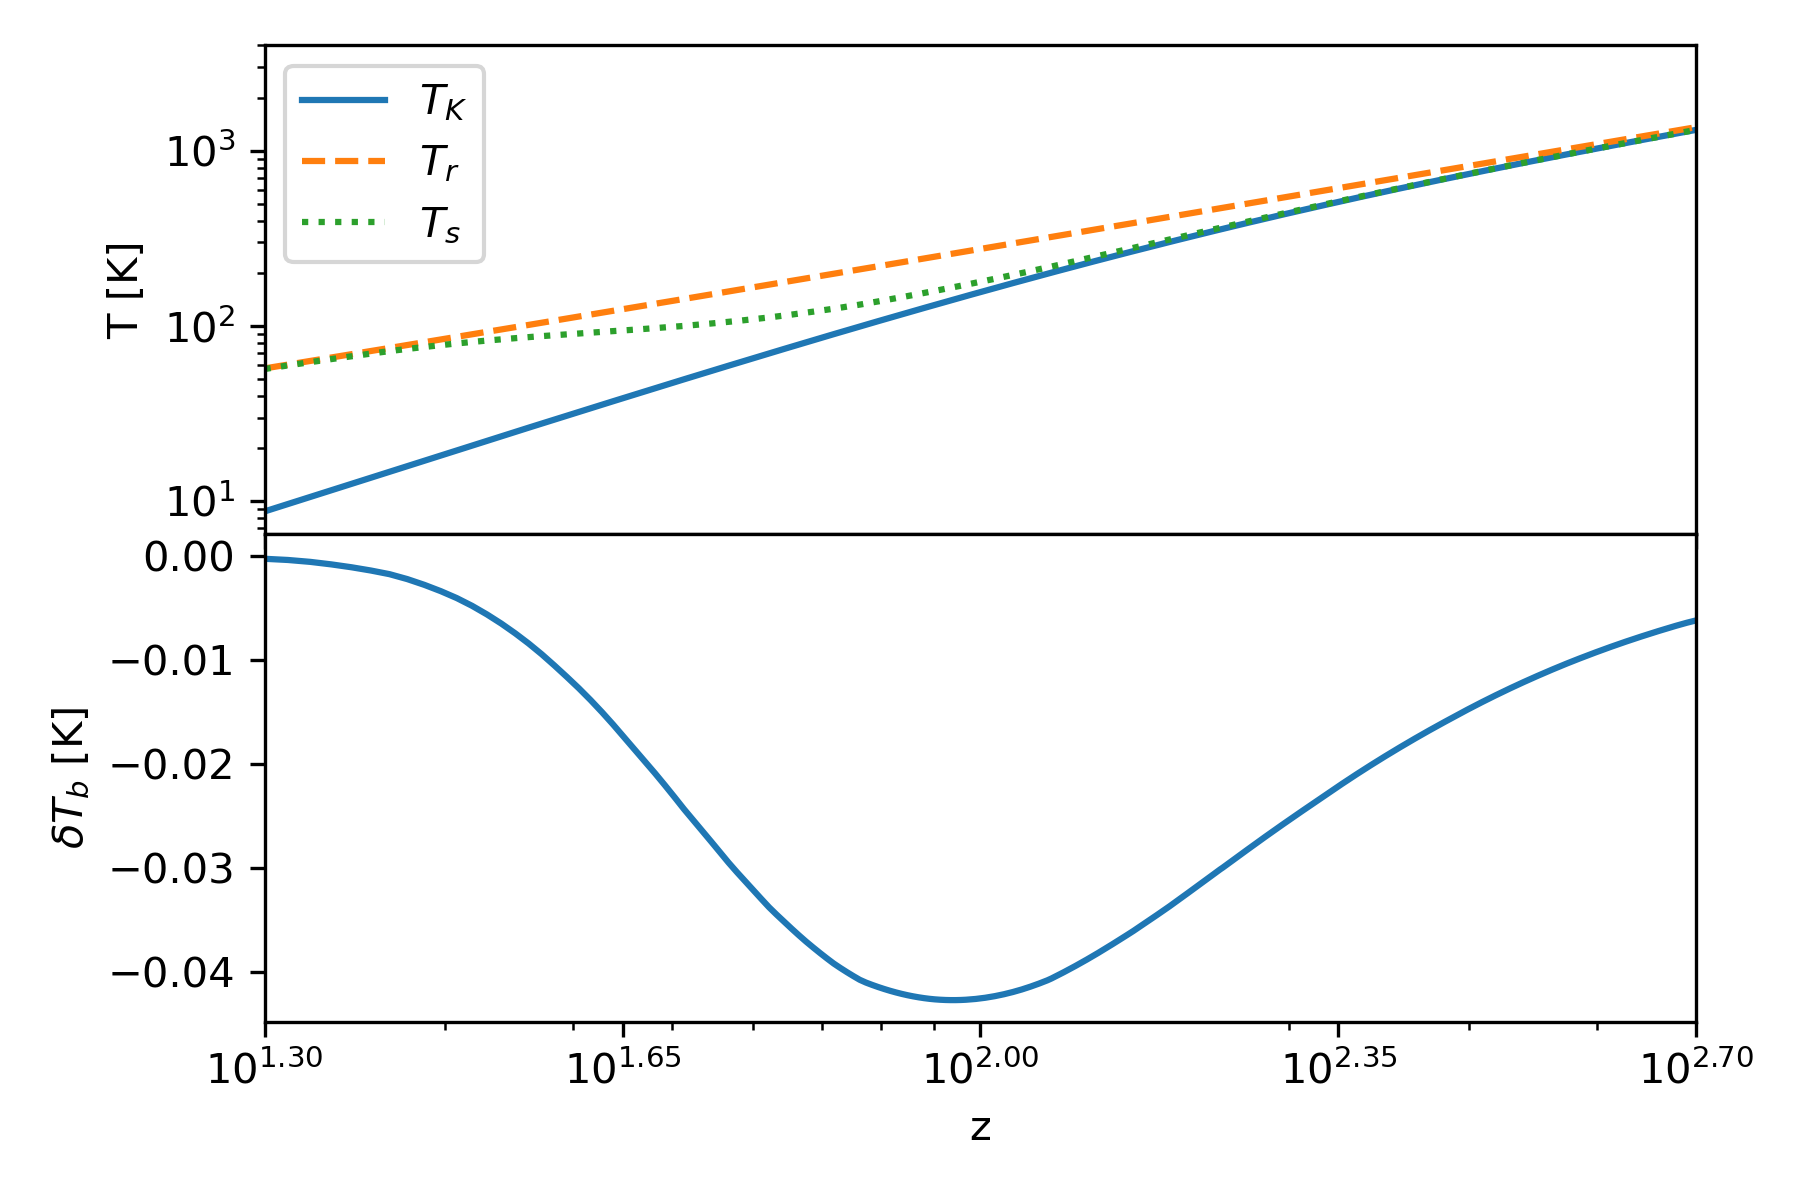
\includegraphics{introduction/figs/example_signal_planck_params.png}
    \caption{The dark ages sky-averaged 21-cm signal. The top panel shows the relationship and evolution of the radio background (orange dashed line), gas temperature (blue solid line) and spin temperature (green dashed line). The bottom panel shows the dark ages 21-cm signal, which is produced by collisional coupling of the spin temperature to the gas temperature. We assume a $\Lambda$CDM baseline \cite{Planck2018}.}
    \label{fig:dark_ages}
\end{figure}

At this early time, collisional coupling drives the spin temperature to the gas temperature, which as just described is lower than the radio background temperature. This produces an absorption feature in the sky-averaged 21-cm signal shown in \cref{fig:dark_ages}. The collisional coupling coefficient is given by
\begin{equation}
    x_c = \frac{\kappa_{10} n_H T_*}{A_{10} T_r},
\end{equation}
where $\kappa_{10}$ is the rate coefficient for spin deexcitations in collisions between neutral hydrogen atoms and is a function of the gas temperature, $T_k$, and $n_H$ is the neutral hydrogen number density. This process is straightforward to model with analytic solutions. Eventually, as the density of the gas reduces, collisions become more infrequent and the spin temperature decouples from the gas and rises back up to the radio background temperature. Collisional coupling will introduce a peak in the 21-cm power spectrum at high-$z$ on scales corresponding to the mean free path for collisions. This all happens prior to the formation of the first galaxies, and a detection of this signal could inform us about key cosmological parameters. The detection of the dark ages signal is the subject of many upcoming missions to the Moon \cite{Burns_Moon_2021} and is not explored significantly in this work.

Once the first stars begin to form around $z\approx25-50$, the spin temperature is expected to couple once again to the gas temperature via the Wouthuysen-Field effect \cite{Wouthuysen1952, Field1959}. In this process, neutral hydrogen atoms absorb and re-emit Lyman-$\alpha$ photons from the first stars which leads to a change in the hyperfine state of the atom and consequently in the spin temperature. The low energy $1_0 S_{1/2}$ hyperfine state, with anti-aligned electron and proton spins, is excited to one of the two central $2P$ states through the absorption of a Lyman-$\alpha$ photon followed by emission and deexcitation to either of the $n = 1$ states. This process is illustrated in \cref{fig:wouthuysen_field}.

The intensity of the Lyman-$\alpha$ emission is driven by the star formation rate in early galaxies. In semi-numerical simulations, the star formation rate is modelled with a star formation efficiency, $f_*$, and the virial circular velocity of star forming halos, $V_c$ \cite{Cohen_global_2017}. The efficiency is the fraction of gas in dark matter halos that is transformed to stars. $V_c$ is then directly related to the halo mass, $M$, via
\begin{equation}
    V_c = 23.4 \bigg(\frac{M}{10^8h^{-1}M_\odot}\bigg)^{1/3} \bigg[\frac{\Omega_m}{\Omega_m^z}\frac{\Delta_c}{18\pi^2}\bigg]^{1/6}\bigg(\frac{1+z}{10}\bigg)^{1/2} \textnormal{km~s}^{-1},
\end{equation}
derived in \cite{Barkana_mass_2001}. Here $M_\odot$ is a solar mass unit, $\Omega_m$ is the matter density parameter, $\Omega_m^z$ is the equivalent as a function of redshift and $\Delta_c$ is the final overdensity relative to the critical density at the collapse redshift of the halo. The effects of varying the astrophysical parameters in the semi-numerical simulations, with a radio background above the CMB, on the global 21-cm signal are shown in \cref{fig:standard_parameters}.

\begin{figure}
    \centering
    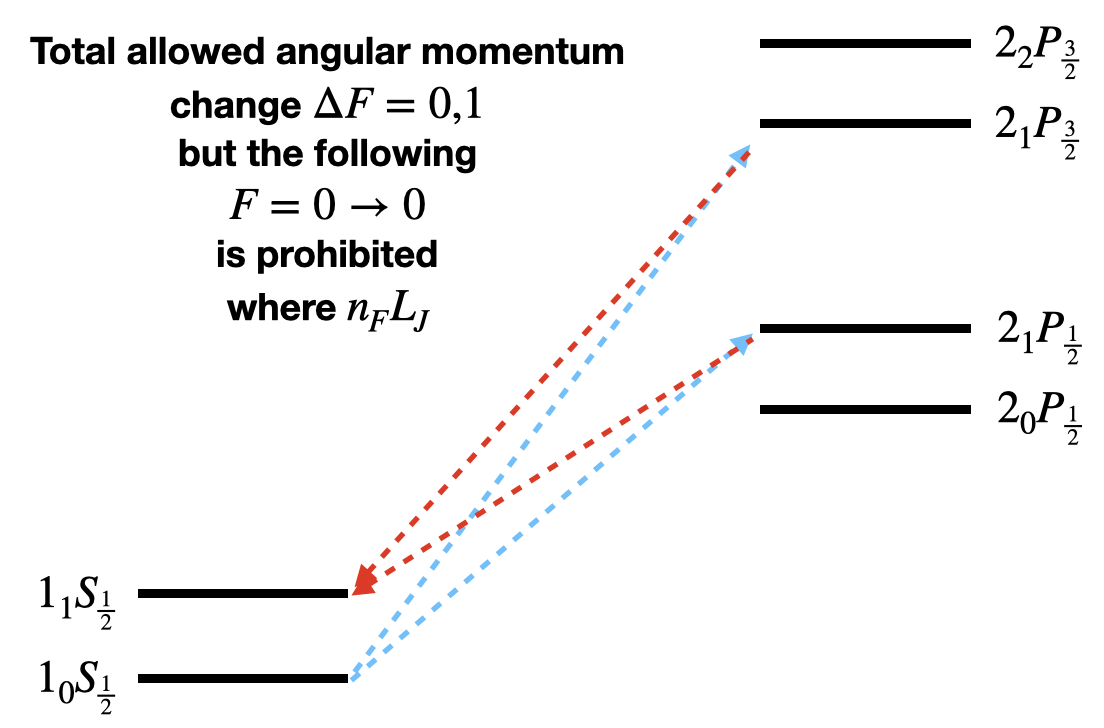
\includegraphics[width=0.8\linewidth]{introduction/figs/Wouthuysen_field.png}
    \caption{The Wouthuysen-Field effect. The absorption and emission of Lyman-$\alpha$ photons by neutral hydrogen drives the spin temperature during the epoch of star formation via the Wouthuysen-Field effect. The blue dashed lines show the absorption of Lyman-$\alpha$ photons and the red show the emission.}
    \label{fig:wouthuysen_field}
\end{figure}

The Wouthuysen-Field effect thus causes an absorption against the radio background between $z\approx20-30$ in the sky-averaged signal, which can be seen in \cref{fig:sky_averaged_signal}, by coupling $T_s$ and $T_k$. In the power spectrum, the Wouthuysen-Field effect manifests itself as a peak at high z and angular scales corresponding to the effective horizon of the coupling process (a few Mpc). In practice, the spin temperature is coupled to the colour temperature, $T_{c}$, but since the IGM is optically thick to Lyman-$\alpha$ emission during this period $T_c \approx T_k$. The coupling coefficient is given by
\begin{equation}
    x_\alpha = \frac{4 P_\alpha T_*}{27 A_{10} T_r},
\end{equation}
where $P_\alpha$ is the total rate at which Lyman-$\alpha$ photons are scattered per atom. $x_\alpha$ is directly proportional to the angular averaged intensity of Lyman-$\alpha$ emission, $J_\alpha$, via $P_\alpha$. During this epoch $T_k$, and the coupled spin temperature, continues to cool at a faster rate than the radio background. However, various heating processes begin when the first stars begin to form raising the gas temperature and preventing $T_k$ from cooling adiabatically. These include Lyman-$\alpha$, X-ray, CMB and shock heating.

\begin{figure}
    \centering
    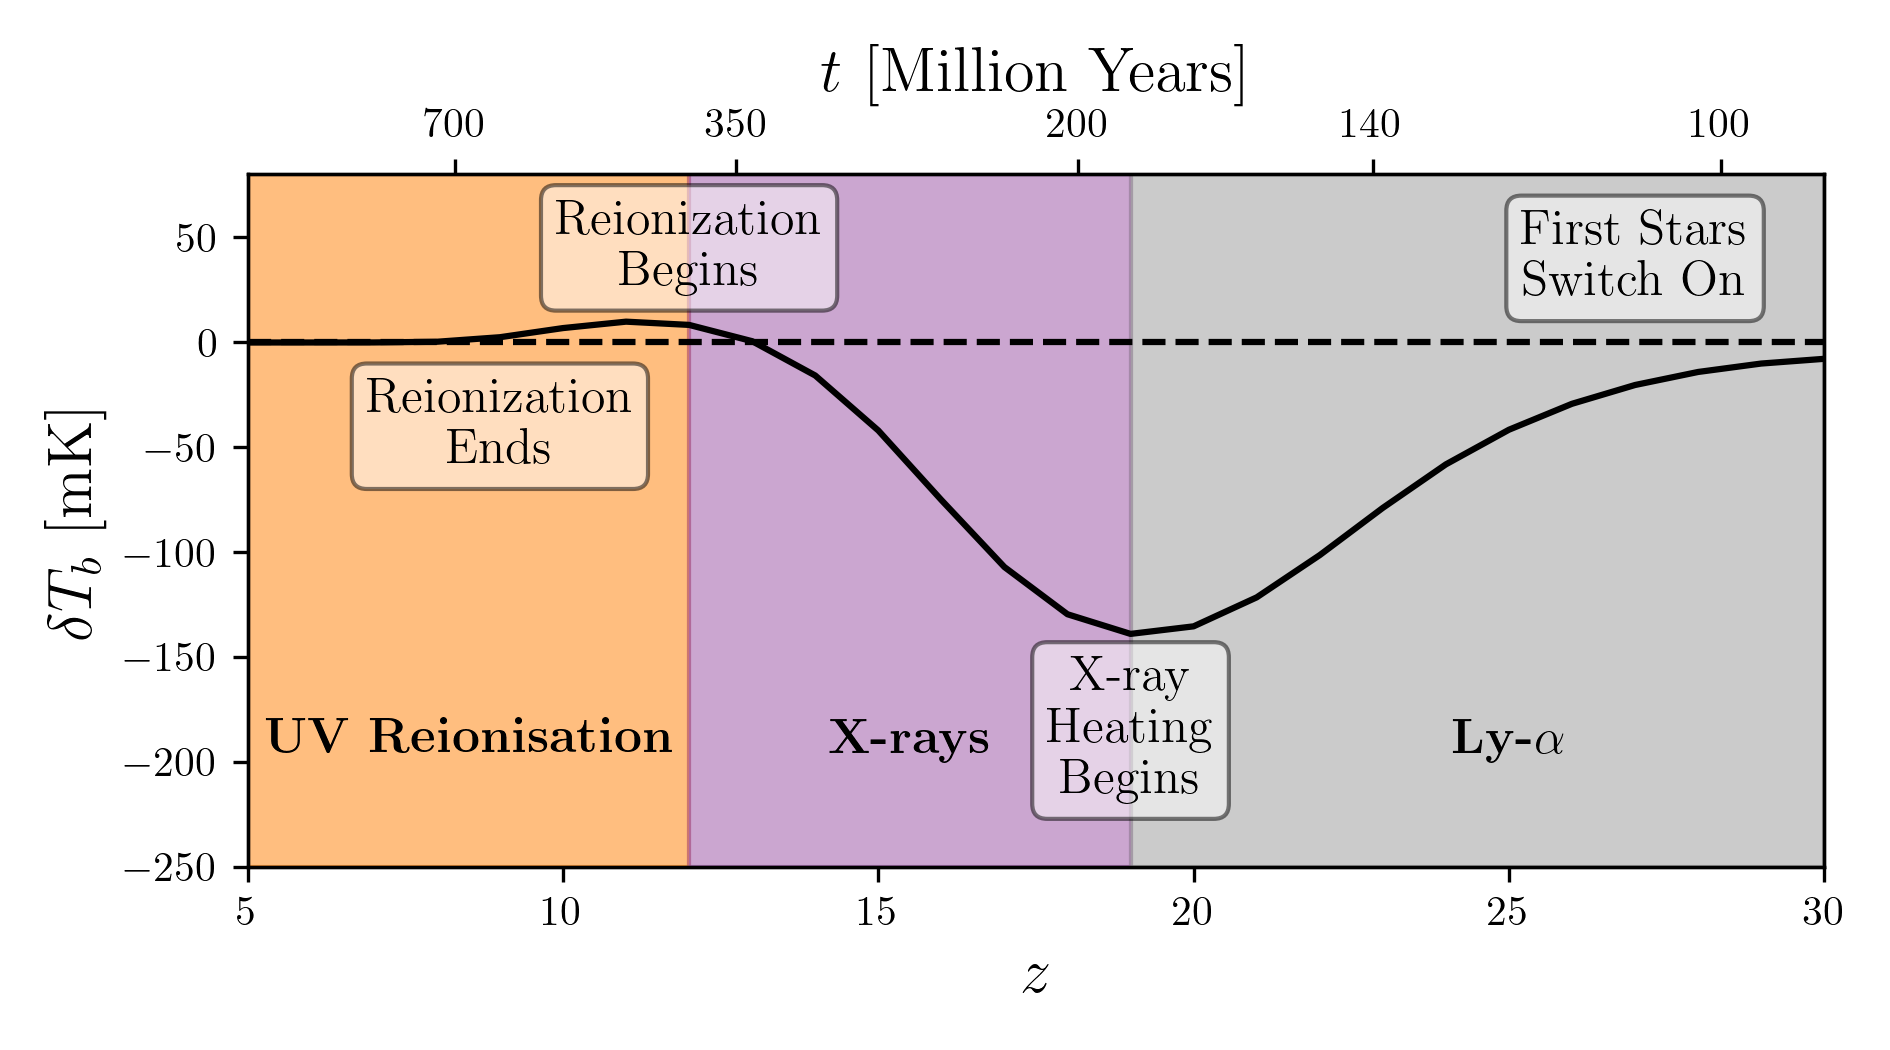
\includegraphics{introduction/figs/signal.png}
    \caption{The 21-cm signal from the Cosmic Dawn and Epoch of Reionization is highly dependent on the intensity of a number of different radiative fields. The figure illustrates the dominant radiative fields as a function of redshift and time after the Big Bang and as a backdrop to an example 21-cm signal. At early redshift, when the first stars switch on, Lyman-$\alpha$ emission drives the spin temperature to the gas temperature, causing an absorption in the signal against the radio background. CMB and Lyman-alpha heating begin to play an important role in modulating the gas temperature and then at later redshifts along with X-ray heating raise the gas temperature back up to and sometimes beyond the radio background temperature. Finally, at more recent times and low redshifts UV emission from stars ionizes the neutral hydrogen and the signal disappears against the radio background. The signal shown here was generated with the neural network signal emulator \textsc{globalemu}, which is discussed in \cref{ch:globalemu}, trained on simulations with a radio background equivalent to the CMB.}
    \label{fig:sky_averaged_signal}
\end{figure}

Lyman-$\alpha$ heating plays a significant role in determining the structure of the global 21-cm signal \cite{Reis_sta_2021}. This mechanism deposits energy in the gas, increasing $T_k$, via the scattering of Lyman-$\alpha$ photons, that induce the Wouthuysen-Field effect, and although the energy deposited per event is small the number of scattering events is large. Since $T_k$ and $T_s$ are coupled at this time, both begin to move back towards the radio background temperature, reducing $\delta T_b$. The Wouthuysen-Field effect still dominates during this period but the heating mechanism significantly reduces the maximum allowed theoretical depth of the global signal from $\approx - 250$~mK to $\approx - 165$~mK \cite{Reis_sta_2021} assuming the radio background is equal to the CMB temperature. This process begins as soon as the first stars form, whereas X-ray heating is delayed until quasars and X-ray binaries begin to form. The heating mechanisms in general suppress the low-$z$ power spectrum peak induced by the Wouthuysen-Field effect \cite{Chuzhoy2007, Villanueva2020, Venumadhav2018, Reis_sta_2021, Mittal2021}.

\begin{figure}
    \centering
    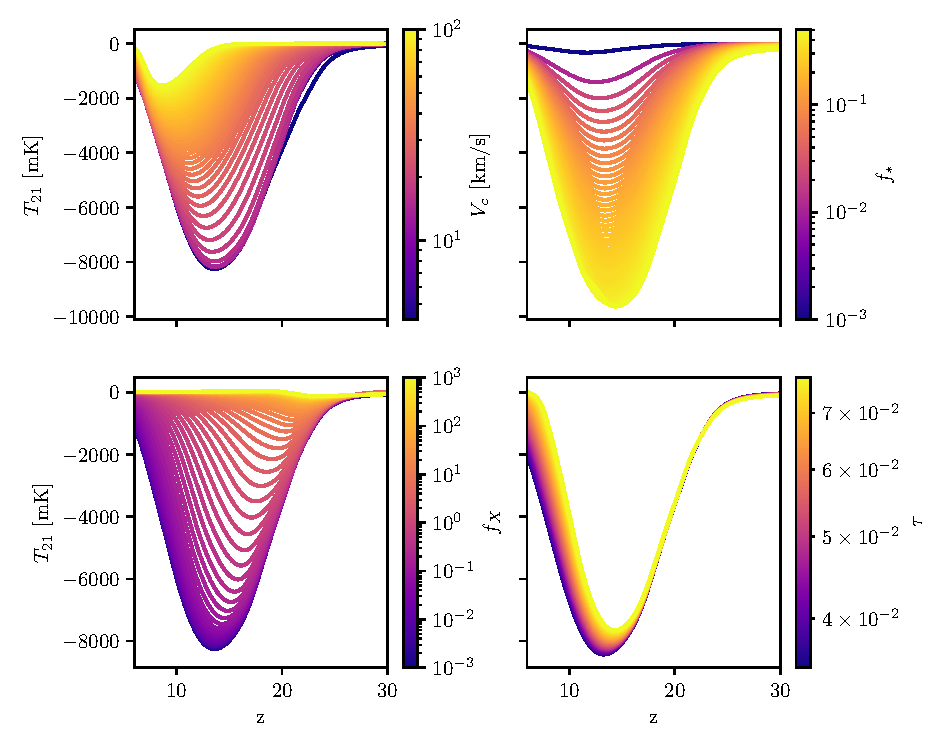
\includegraphics{introduction/figs/other_params_variation.pdf}
    \caption{The figure shows the effect of varying four different parameters of the semi-numerical simulation detailed in the text and throughout this thesis. The base signal that is varied has strong star formation, inefficient X-ray heating and a strong radio background. The simulations have an excess radio background above the CMB from high redshift radio galaxies. The minimum virial circular velocity, $V_c$, and the star formation efficiency, $f_*$, determine the star formation rate and consequently the Lyman-$\alpha$ flux. Low values of $V_c$ and high values of $f_*$ lead to high Lyman-$\alpha$ fluxes, strong coupling between the spin temperature and the gas temperature, and as a result deep 21-cm signals. It also influences the onset of heating, however this is harder to disentangle from X-ray heating. X-ray heating is governed by the X-ray efficiency, $f_X$, in these simulations. Low values of $f_X$ lead to inefficient X-ray heating and push the minimum of the global 21-cm signal down and to lower redshifts. Finally, we show the variation in the signal with the CMB optical depth, $\tau$, which has very little influence in the structure of the signal at high redshift but becomes more important at low redshift during the Epoch of Reionization. It's important to note that these effects are not independent and do not occur at distinct epochs but rather overlap, meaning that the structure of the signal as a function of redshift is complex. However, figures like this help to gain an intuition for how each parameter affects the structure of the signal. Again, the signals were produced with the neural network emulators discussed primarily in \cref{ch:globalemu} and then also in \cref{ch:saras2} and \cref{ch:saras3}.}
    \label{fig:standard_parameters}
\end{figure}

A related heating mechanism is CMB heating, in which energy is transferred from the radio background to the gas via interactions with neutral hydrogen. In CMB heating, a CMB photons raise the energy state of the electron in the neutral hydrogen atom from $1_0$S$_{1/2}$ to $1_1$S$_{1/2}$ and the neutral hydrogen atom subsequently scatters with a Lyman-$\alpha$ photon. The scattering raises the electron into one of the 2P states and then the electron can deexcite back into the $1_0$S$_{1/2}$ releasing a higher energy Lyman-$\alpha$ photon in the process. The additional energy has come from the CMB photon and is transferred by the Lyman-$\alpha$ photon to the gas thus raising the gas temperature~\cite{Venumadhav2018}. CMB heating can reduce, $x_r$ which is dependent on the 21-cm optical depth
\begin{equation}
    x_r = \frac{1 - \exp(-\tau_\nu)}{\tau_\nu},
\end{equation}
below 1 \cite{Reis_sta_2021}.

Further heating occurs through IGM shocks. As the Universe expands the density fluctuations seen in the CMB grow to form galaxies and large scale structure. However, these density fluctuations are not spherical and so collapse into sheets or ``Zel'dovich pancakes'', filaments and halos. During this process of collapse, if the velocity of the infalling gas is higher than the speed of sound, some of the gravitational infall energy is transformed into thermal energy via shocks. Shocks are only important when the temperature of the shock, $T_\mathrm{sh}$, is greater than $T_k$ and the temperature scales as the mass of the collapsing region to the power of six. The process plays a more significant role at high redshift but the energy transferred to the IGM through shocks reduces with increasing time and is generally thought to be minimal throughout the CD and EoR \cite{Furlanetto_review_2006, Mesinger2019}.

Finally, X-ray heating plays a significant role in the structure of the global 21-cm signal. It produces a peak in the power spectrum as a function of redshift and at the relevant galactic and intergalactic scales. X-ray heating is expected to begin around redshifts 15-20. Low energy X-rays and some high energy X-rays with long mean free paths from Galaxies and quasars are absorbed by the IGM and deposit most of their energy as kinetic energy raising the gas temperature, $T_k$, which at this time is still coupled to the spin temperature via the Wouthuysen-Field effect. Further, the X-rays photoionize hydrogen and helium in the IGM with the resulting free electrons retaining the majority of the photon energy as kinetic energy. This kinetic energy is subsequently deposited into the IGM via collisional ionization and excitation of helium and hydrogen. Collisional ionization leads to a background of secondary electrons that subsequently deposit kinetic energy into the IGM and excitation of helium creates a background of photons that go on to ionize hydrogen. Collisional excitation of hydrogen in turn produces a background of Lyman-$\alpha$ photons which can heat the gas through the process described above. Finally, the free electrons created by X-ray photoreionization of hydrogen can heat the IGM through Compton collisions with other free electrons.

The high redshift X-ray background is poorly understood and in the semi-numerical simulations employed throughout this thesis it is assumed that the relationship between the X-ray luminosity and the star formation rate at low redshifts can be extrapolated, taking into account an increase in luminosity with decreasing metallicity, to high redshifts. Between 0.2 - 10 keV the luminosity is given by
\begin{equation}
    L_X = 3\times 10 ^{40} f_X \bigg(\frac{\mathrm{SFR}}{1 M_\odot \mathrm{yr}^{-1}}\bigg) \mathrm{erg~s}^{-1},
\end{equation}
where $f_X$ is the efficiency of X-ray production in high redshift galaxies, effectively acting as a normalisation parameter, and a free parameter in our models. We model the spectrum of X-ray sources in the simulations under the assumption that they are predominantly X-ray binaries in which stellar mass from a main sequence star accretes onto a neighbouring compact object. These systems should be prominent in the early Universe and should form as the first population of stars begins to die. We characterise the spectra of the X-ray binaries either empirically from \cite{Fragos_Xrays_2013} or analytically with two free parameters in our semi-numerical simulations; $\nu_\mathrm{min}$ (occasionally referred to $E_\mathrm{min}$) which is the low energy cut-off of the spectral energy density and $\alpha$ which is the slope of the spectral energy density. %The modelling of the X-ray background is limited and additional contributions from for example quasars are not included, however it is expected to be sufficient for current requirements. 
In some instances, X-ray heating can be sufficiently large to raise the gas temperature and coupled spin temperature above the radio background temperature, as can be seen in \cref{fig:sky_averaged_signal}.

At lower redshifts, reionization, in which neutral hydrogen is ionized via UV emission from the first stars, begins to dominate the structure of the 21-cm signal during the Epoch of Reionization. Once all the hydrogen is ionized and the neutral fraction of hydrogen in \cref{eq:bright_temp}, $x_{HI} = 0$, then the signal disappears against the radio background. Reionization occurs first around the sources of UV emission and is dependent on the mean free path, $R_\mathrm{mfp}$, of the ionizing radiation which is a free parameter in the semi-numerical simulations. The total column density of the ionizing gas is measured by the CMB optical depth $\tau$ which is proportional to the ionizing efficiency of sources, $\zeta$. Again, $\tau$ is a free parameter in the simulations. It has previously been constrained by Planck, however, its value remains uncertain with a strong dependence on the reionization model. The 21-cm line offers an alternative means by which it can be constrained. UV reionization begins as soon as the first stars form and UV photons in the Lyman-Werner band deplete the amount of neutral hydrogen that can go into stars via ionization thus suppressing star formation in a process known as Lyman-Werner feedback \cite{Cohen_global_2017}. However, the strength of this feedback mechanism is not well understood \cite{Visbal_lw_2014}.

Typically, the radio background in simulations of the 21-cm signal is set to the CMB temperature. However, we know that radio galaxies should contribute to this background. Further, measurements from the balloon experiment Absolute Radiometer for Cosmology, Astrophysics, and Diffuse Emission~(ARCADE2) \cite{fixsen_arcade_2011} and the Long Wavelength Array~(LWA) \cite{dowell_radio_2018} suggests that there is a radio background in excess of the CMB which can be modelled as a homogeneous synchrotron source. However, there are concerns about the galactic modelling in the two experimental measurements of the excess \cite{Subrahmanyan2013}. The reported detection from the EDGES experiment in 2018 also hints at the possibility of an excess radio background, however there are concerns about the modelling of the EDGES data (see \cref{sec:current_results}). A larger radio background leads to a stronger contrast with the spin temperature and consequently a deeper absorption feature in the global 21-cm signal and a larger power spectrum.

\begin{figure}
    \centering
    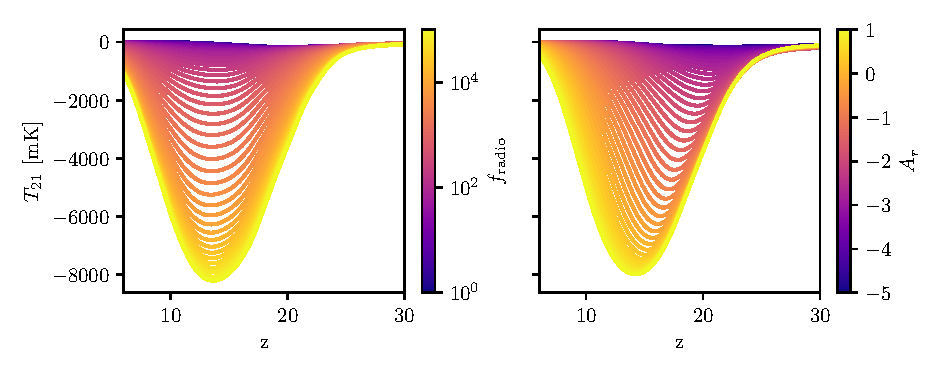
\includegraphics{introduction/figs/backgrounds_variation.pdf}
    \caption{The figure shows the variation of two different parameterisations of  exotic global 21-cm signals with excess radio backgrounds. In both figures the star formation rate is high (with a high star formation efficiency and low minimum virial circular velocity) and the X-ray efficiency is low, which along with a large radio background produces a deep signal. The CMB optical depth is set to 0.05 and its value is only important at low redshifts. The left-hand panel corresponds to an excess radio background above the CMB produced from radio galaxies and mediated by the radio production efficiency, $f_\mathrm{radio}$, which is proportional to the radio luminosity per star formation rate, $L_r/\mathrm{SFR}$. The right-hand panel corresponds to an excess from a homogeneous synchrotron source and its magnitude is mediated by $A_r$ which is effectively the fractional increase on the CMB at a given frequency (here 78 MHz). The excess radio background models were originally proposed to explain the anomolously deep EDGES absorption feature reported in 2018. More details can be found in the text. The signals were generated using the neural network emulator detailed in \cref{ch:globalemu}, \cref{ch:saras2} and \cref{ch:saras3}.}
    \label{fig:radio_parameters}
\end{figure}

Throughout the later chapters of this thesis, we use semi-numerical simulations with two different parametrisations of an excess (over the CMB) radio background. The first is from a synchrotron source which produces a uniform radio background
\begin{equation}
    T_\mathrm{r} = T_\mathrm{CMB}\bigg[ 1 + A_{\mathrm{r}}^{78}\bigg(\frac{\nu}{78\textnormal{MHz}}\bigg)^\beta\bigg],
    \label{eq:srb_background}
\end{equation}
that decays with increasing time. Here $A_r$ is a fractional increase on the CMB at a given frequency, and it can be scaled according to
\begin{equation}
    A_{\mathrm{r}}^{78} = A_{\mathrm{r}}^{1420} \bigg(\frac{0.078}{1.420}\bigg)^\beta,
\end{equation}
where $\beta$ is often chosen to be equal to $-2.6$ consistent with measurements from ARCADE2 and LWA. This model has a larger impact on the global 21-cm signal at higher redshifts and generally pushes the minimum of the global 21-cm signal to higher redshifts which can be seen in \cref{fig:radio_parameters}. The synchrotron excess may be sourced by superconducting cosmic strings \cite{Brandenberger2019} or light dark matter decays \cite{Fraser2018, Pospelov2018}. Since the radio background is homogeneous, it leads to an increase in the power spectrum at all angular scales, but its impact is again more significant at high redshifts.

The second parameterisation of the radio background is from high redshift radio galaxies. In this instance the radio background is modelled via the radio production efficiency, $f_\mathrm{radio}$, which is proportional to the radio luminosity per star formation rate
\begin{equation}
L_r	= 10^{22} f_\mathrm{radio} \bigg(\frac{\nu}{150~\mathrm{MHz}}\bigg)^\beta \bigg(\frac{\mathrm{SFR}}{M_\odot~\mathrm{yr}^{-1}}\bigg)~\mathrm{W~Hz}^{-1},
\end{equation}
where again $\beta$ is usually set to $-2.6$. The level of excess background above the CMB in this model increases with decreasing redshift, in contrast to the previously discussed model, as more radio galaxies form. It is also non-uniform unlike the synchrotron model. This non-uniformity leads to an increase in the power spectrum on angular scales corresponding to galactic and intergalactic length scales. The model has a similar effect on the depth of the global 21-cm signal to the synchrotron model creating a stronger contrast between $T_s$ and $T_r$. However, as can be seen in \cref{fig:radio_parameters}, it does not affect the redshift of the minima in the global signal.

Since the 21-cm signal is highly dependent on the amplitude of a number of different radiation fields, it is a powerful probe of the infant Universe and the first galaxies. Its detection represents one of the final frontiers in observational cosmology, along with studies of dark energy, dark matter and gravitational waves. In the later chapters of this thesis, we present the current best limits on the properties of early galaxies from 21-cm cosmology, but presently we describe the challenges of making a detection.

\section{Challenges facing the field}

There are a number of different challenges facing the field of 21-cm cosmology, and we detail several specific issues in the following subsections. This is followed by a more general discussion of `unknown systematics' in which we group together additional challenges that if incorrectly dealt with can introduce non-smooth structure into the data that mimics, corrupts or hides the global 21-cm signal. We focus on the detection of the sky-averaged 21-cm signal here, as that is the main focus of the thesis, but note that there are similar challenges and unique problems in studies of the power spectrum.

\subsection{Galactic, extra-galactic foregrounds and the antenna beam}
\label{sec:foregrounds}

Radiometers aiming to detect the sky-averaged 21-cm signal also pick up emission from the Galaxy and from other galaxies, which dominates over the order $100$~mK cosmological signal. This foreground is composed of synchrotron and free-free emission and is approximately five orders of magnitude larger than the 21-cm signal, as can be seen in \cref{fig:relative_signal_magnitudes}. The foregrounds are expected, from the theory of synchrotron and free-free emission, to be smooth and follow an approximate $\nu^{-2.5}$ power law. SARAS3 found that the sky had a spectral index of $-2.42$ \cite{SARAS3}, EDGES found it to be approximately $-2.6$ as a function of local sidereal time \cite{Mozdzen_EDGES_spectral_index_2017}, and LEDA reported a measurement of the spectral index to be $\beta = -2.5 \pm 0.1$ \cite{LEDA_spectral_Index_2021}.

\begin{figure}
    \centering
    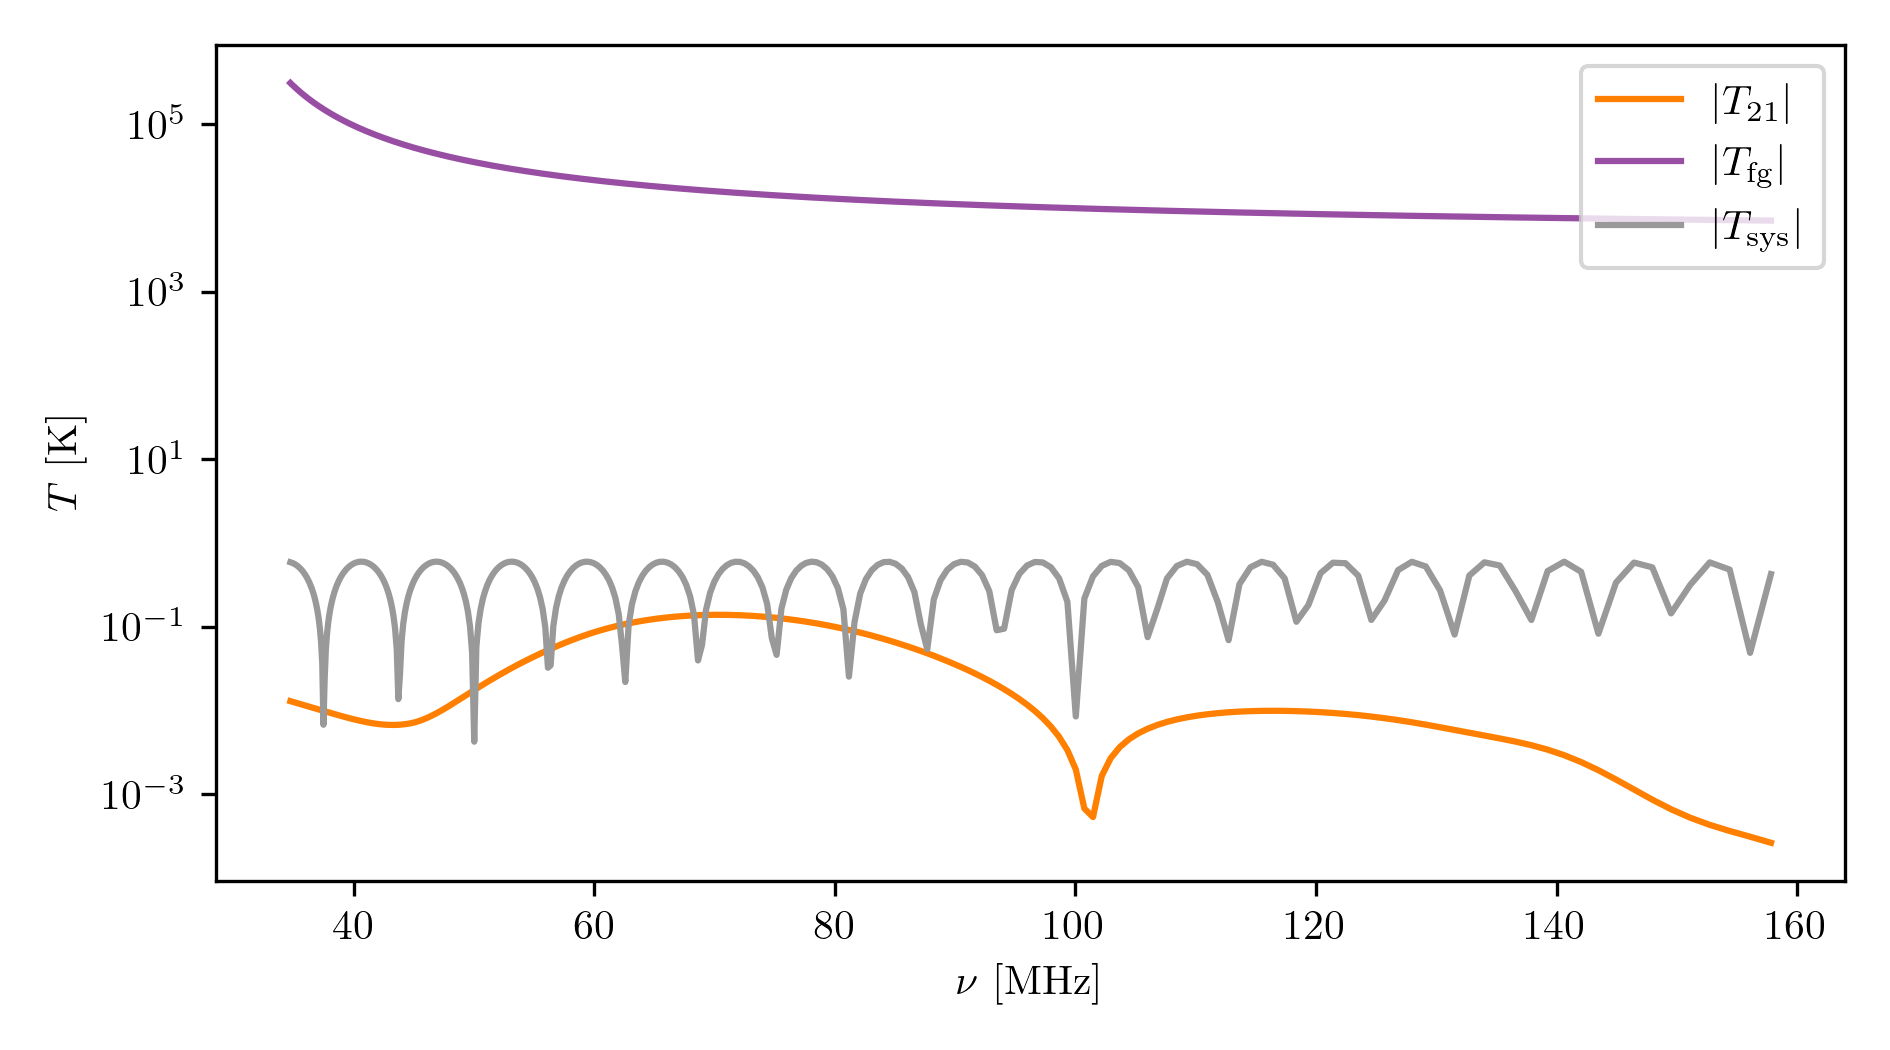
\includegraphics{introduction/figs/the_data.png}
    \caption{The graph shows the relative magnitude of different signals collected by global 21-cm experiments. The foregrounds (purple) are around five orders of magnitude larger than the 21-cm signal (orange). Sinusoidal systematics are frequently found in the data from these experiments and can be caused by cable reflections, chromaticity in the beam and discontinuities in the soil among other things discussed in the text. We show an example systematic (grey) to illustrate that these signals have similar magnitudes to the 21-cm signal and need to be corrected for.}
    \label{fig:relative_signal_magnitudes}
\end{figure}

Since the foreground dominates so significantly over the 21-cm signal, it is essential that the two signals can be separated from each other. To do this, we often take advantage of the fact that the foreground is smooth, and the signal is not over a wide frequency (or equivalently redshift) range. The idea is that we model the smooth structure in the data with a low order polynomial function, often in log-space,
\begin{equation}
    \log_{10}T_\mathrm{fg}(\nu) = \sum_i^N a_i \log_{10}(\nu)^i,
\end{equation}
where the coefficients $a_i$ are fitted for, to leave behind the non-smooth 21-cm signal. Alternative physically motivated polynomial models have also been proposed, however their applications have been limited \cite{Bowman_edges_2018}.

There are however complications with the principle of separating smooth foregrounds from the non-smooth signal with polynomials. It requires the design of a wideband instrument, since over narrow frequency ranges the 21-cm signal is also smooth and easily modelled by low order polynomials. Whilst designing a wideband antenna is possible, this leads to a very non-smooth response from the antenna to the sky, which can be difficult to correct for. This effect in the antenna beam is known as chromaticity and is a major issue for 21-cm experiments.

In \cref{fig:chromaticity}, we illustrate how the structure of the antenna beam affects the recorded data. We use an elliptical dipole above an infinite ground plane shown in the bottom right of the figure to illustrate, along the top row, how a slice through the beam at a fixed azimuthal angle changes with frequency from $50 - 200$~MHz. We then posit the existence of two bright sources in the sky, shown by the purple and orange stars, which have smooth spectra that are power laws in frequency with $\beta \approx -2.5$ as shown by the orange and purple dashed lines in the figure on the bottom left. The incoming radiation from these two bright sources is effectively along the line of sight because they are so distant that radial emission is not seen by the antenna.

\begin{figure}
    \centering
    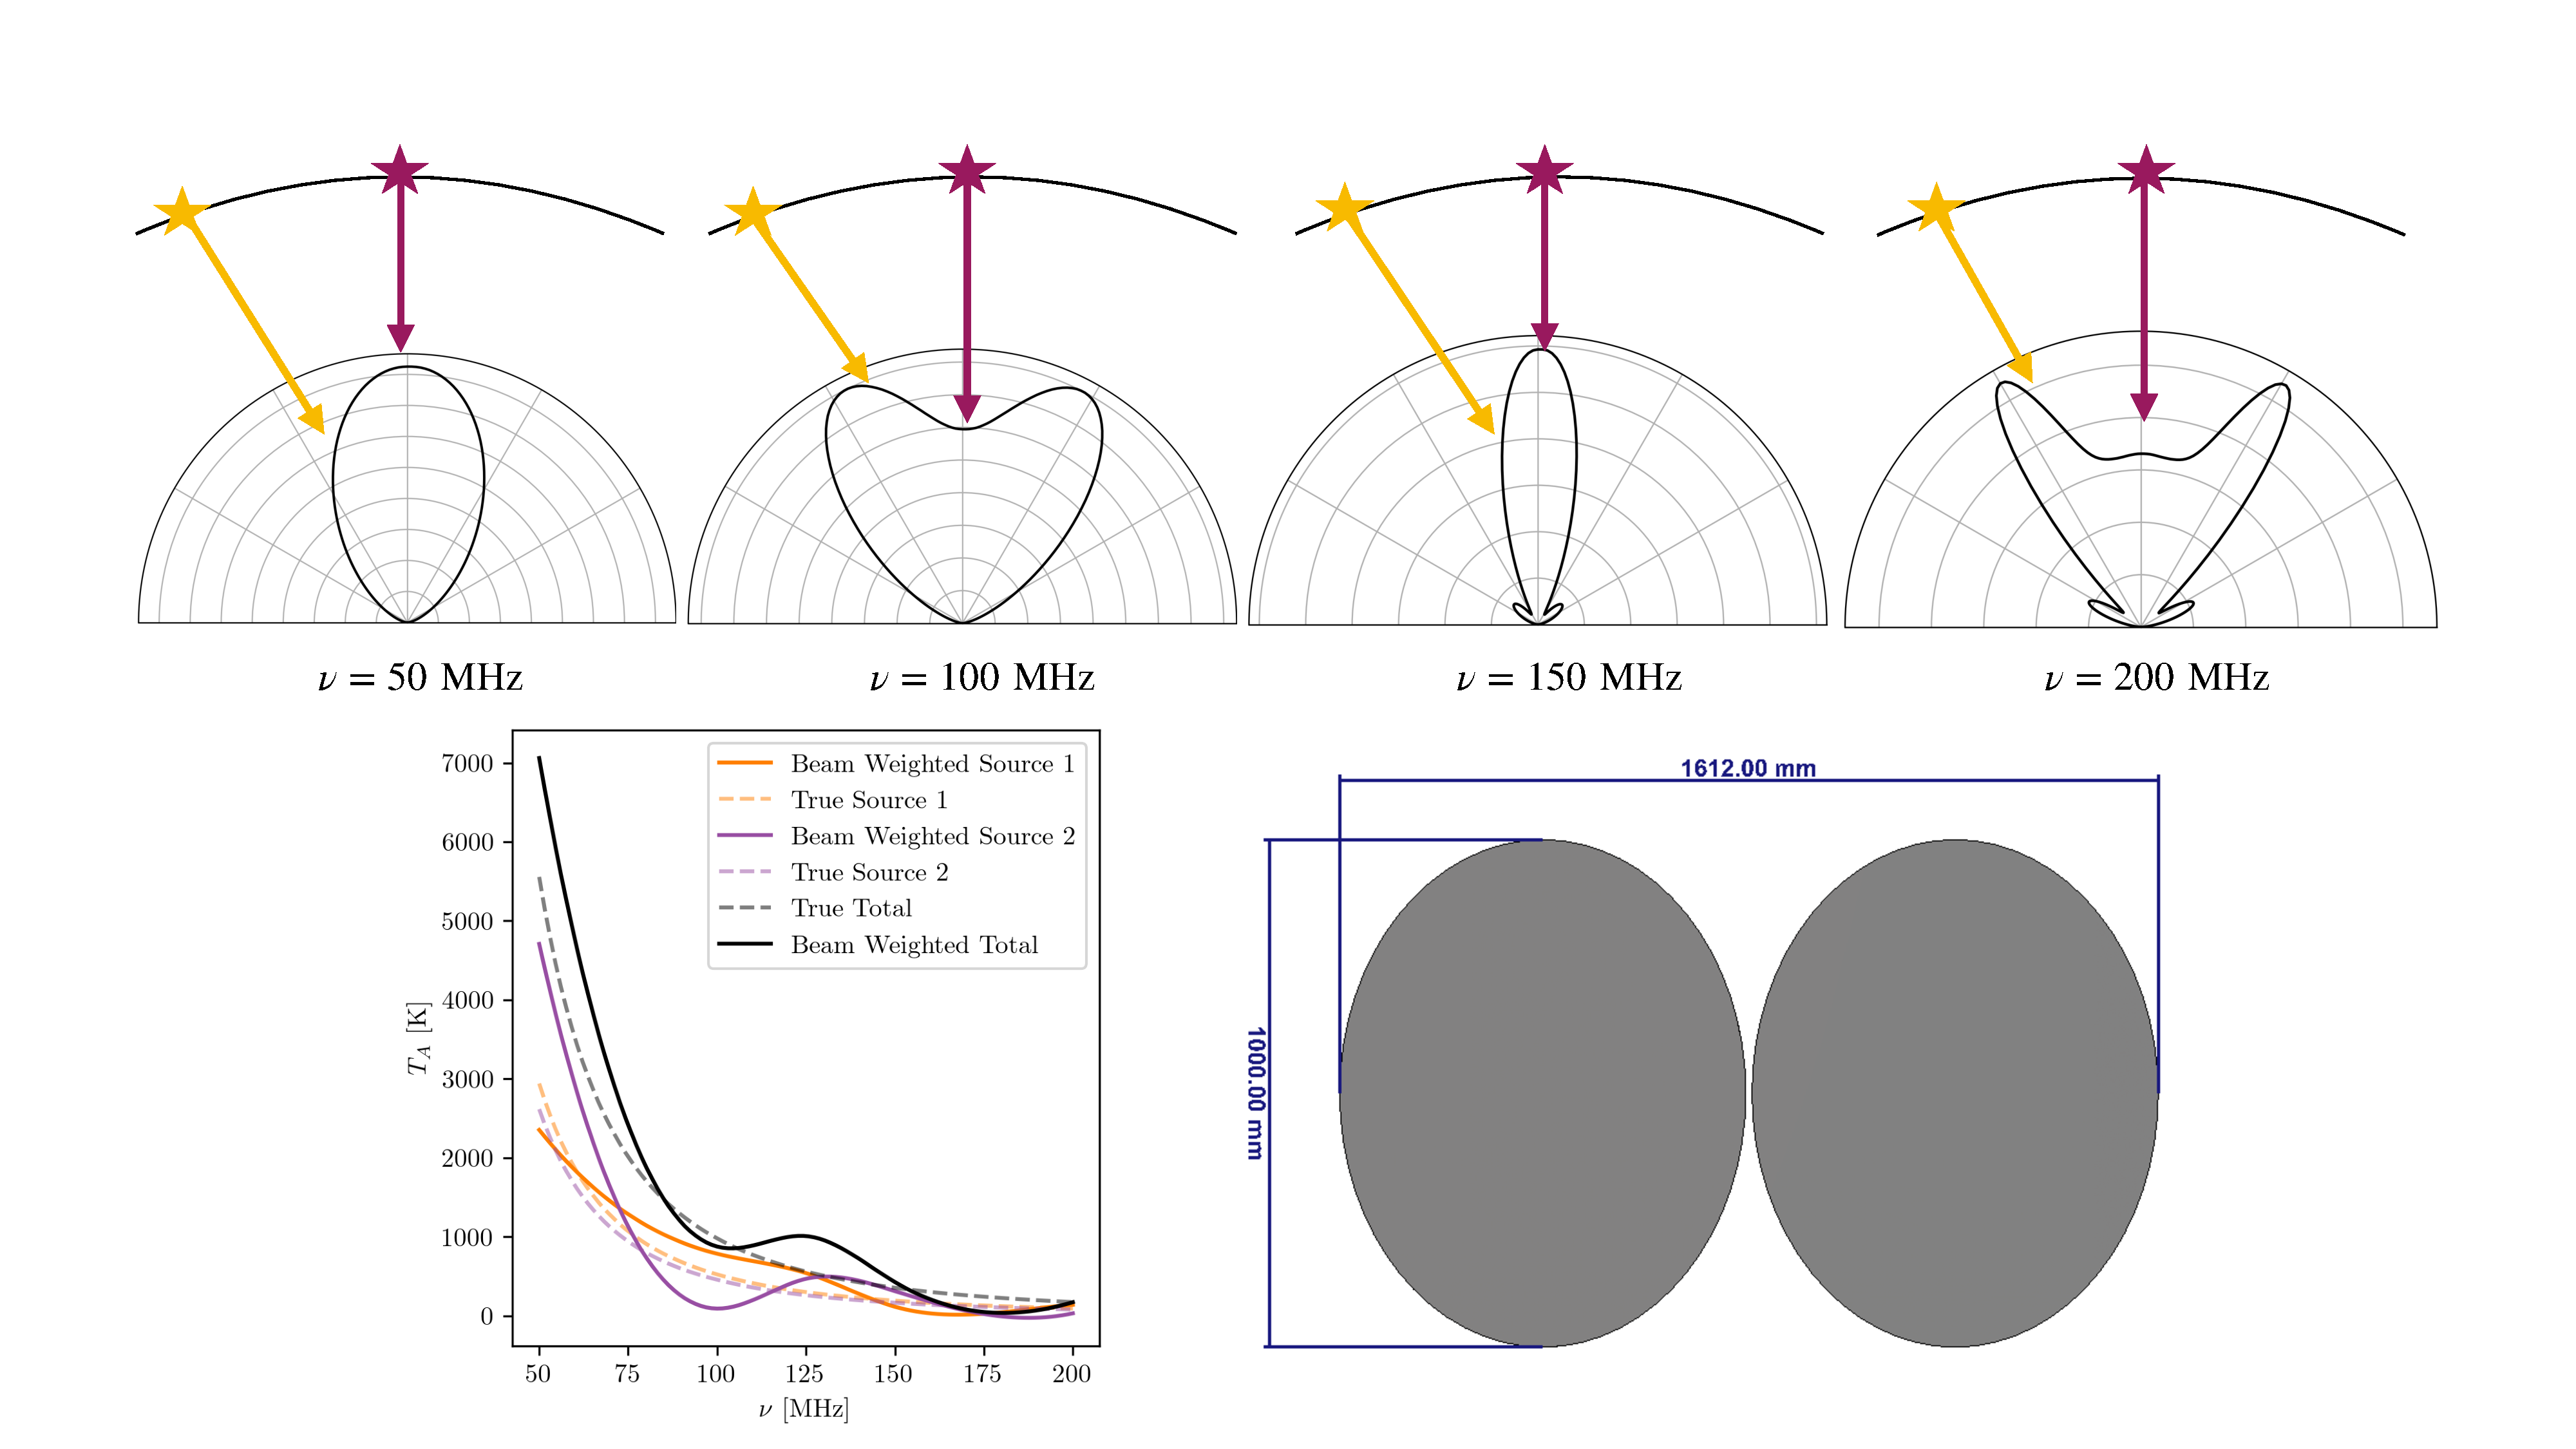
\includegraphics[width=\linewidth]{introduction/figs/chromaticity.pdf}
    \caption{The figure illustrates the impact of a chromatic beam on the sky-averaged 21-cm signal. The bottom right panel shows a Computer Simulation Technology~(CST) model of an elliptical dipole antenna, provided by Dominic Anstey and John Cumner. Along the top row, we show slices through the beam at four fixed frequencies in the range of interest for a 21-cm experiment. The structure of the beam changes with frequency and this causes signals from the sky to be down-weighted at some frequencies relative to others. To illustrate this, we show two different point sources, which we assume to have approximate power law spectra, and how they interact with the beam. The bottom left-hand panel shows the ``true spectrum'' for each source as dashed lines and the recorded spectra as solid lines. We also show the sum of these two point source spectra in black. The beam introduces significant non-smooth structure into the data and this needs to be appropriately modelled so that the 21-cm signal can be recovered from the data. In practice, the problem is much more complicated because the beam is three-dimensional, the sky is full of complex structure and the sky varies with time.}
    \label{fig:chromaticity}
\end{figure}

The beam weights the input power from the sky, $T_\mathrm{sky}$, based on its directivity which as can be seen in the top row is a function of angle and frequency. The solid orange and purple lines in the bottom left panel show the weighted spectra which feature chromatic distortion, where the weighting has been exaggerated for demonstration, from the two posited point sources. This can also be seen in the sum of the spectra, shown in black.

In practice, the problem is much more complicated because the beam is 3D, the sky is rich in complex structures such as the galactic plane, the north galactic spur and bright sources such as Cygnus A, and observations are taken over long periods in which the sky rotates above the beam. However, from the simple example we can clearly see how the beam can introduce non-smooth structure into the antenna temperature, $T_A$, and how modelling the foreground in wideband data with a smooth low-order polynomial will leave behind both the non-smooth signal but also a large non-smooth chromatic residual.

One approach to deal with chromaticity is to fit high order polynomials in an effort to model the foreground and the non-smooth chromatic structure in the data. However, this can of course fit out the 21-cm signal as well.

More complete approaches to modelling the effects of chromaticity can be taken. For example, the EDGES collaboration \cite{Mozdzen_EDGES_spectral_index_2017} proposed a correction given by
\begin{equation}
    B(\nu, t) = \frac{\int_\Omega T_\mathrm{sky-model}(\nu_\mathrm{ref}, t, \theta, \phi) D(\nu, \theta, \phi) d\Omega}{\int_\Omega T_\mathrm{sky-model}(\nu_\mathrm{ref}, t, \theta, \phi) D(\nu_\mathrm{ref}, \theta, \phi) d\Omega},
\end{equation}
where $D$ is the directivity of the antenna, $t$ is the time, and $\theta$ and $\phi$ are the zenith and azimuthal angles parameterising the beam. The sky temperature is modelled by the difference between a map and the CMB scaled by a signal power law
\begin{equation}
    T_\mathrm{sky-model} (\nu_\mathrm{ref}, t, \theta, \phi) = [T_\mathrm{base-map} - T_\mathrm{CMB}]\bigg(\frac{\nu_\mathrm{ref}}{\nu_\mathrm{base-map}}\bigg)^{-2.5}.
\end{equation}
The corrected antenna temperature is then given by
\begin{equation}
    T_\mathrm{cor} = \int_{t_\mathrm{start}}^{t_\mathrm{end}} \frac{T_\mathrm{data} - T_\mathrm{CMB}}{B} dt + T_\mathrm{CMB}.
\end{equation}
However, this correction assumes an exact knowledge of the foreground and the antenna beam pattern. In practice the foreground maps are not known well enough and while we can model the antenna beam it is difficult to account fully for the environment around the antenna and for imperfections in manufacturing.

A sophisticated forward modelling of the antenna beam and the foreground has been proposed in a series of papers \cite{Anstey_REACH_2021, Anstey_antenna_2022, Anstey_lst_2022}. The model uses a base sky map which is divided into $N$ regions of varying spectral index and convolved with a model of the beam
\begin{equation}
    T_\mathrm{fg} = \frac{1}{4\pi}\int_0^{4\pi} D(\nu, \theta, \phi) \int_{t_\mathrm{start}}^{t_\mathrm{end}} \sum_{i=0}^{N} M_{i}(\theta, \phi)[T_\mathrm{base-map} - T_\mathrm{CMB}]\bigg(\frac{\nu}{\nu_\mathrm{base-map}}\bigg)^{-\beta_i} dt d\Omega + T_\mathrm{CMB},
\end{equation}
where $M_i(\theta, \phi)$ is the mask that divides the sky map into $N$ regions of identical spectral index $\beta_i$. Work is currently ongoing on a model for any deviation in the beam from the simulations caused by environmental and manufacturing errors.

Ground plane artefacts can be introduced in the data by finite edges or discontinuities in the structure, which are usually hard to model \cite{Bradley_EDGES_2019}. These can produce standing waves on the finite edges of the ground plane and introduce ripples that are unaccounted for in the modelling of $D(\nu, \theta, \phi)$. Ground planes are typically employed for dipole antennas to prevent the antenna looking at the ground with the same efficiency that it looks at the sky, however emission from the soil can still cause problems and discontinuities in the soil structure can also distort the directivity of the antenna.

The 21-cm signal is also affected by chromaticity, but the foregrounds change on much larger length scales and the intensity of the foregrounds vary much more across the sky. We can therefore generally ignore chromatic effects in the sky-averaged 21-cm signal.

Power spectrum experiments also struggle with the effects of the antenna beams and the foregrounds. For example, a major cause of systematics in these experiments is cross-talk between different antennas in the interferometric array. Cross-talk occurs because antennas re-radiate reflected signals, and this can be picked up by neighbouring antennas in the often closely packed array. A detailed discussion of the systematics in power spectrum experiments and how these experiments deal with foregrounds is beyond the scope of this thesis. Briefly, however, one of the most effective ways of dealing with foregrounds in power spectrum experiments takes advantage of the fact that the foreground and 21-cm signals appear on different angular scales and different redshifts meaning that the foregrounds can be avoided by looking at small angular scales at late times. 

In global or sky-averaged experiments we can try to avoid chromatic effects, however, this is very difficult even with a narrowband instrument. Such antennas have frequency independent beams and are known as achromatic antennas. Currently, there is only one collaboration, SARAS, attempting to build such antennas. They are relying on monopole antennas and observing over narrow bandwidths. 

It has been shown via simulations that the SARAS2 instrument has an approximately achromatic response to the sky over the redshift range $z\approx7-12$ \cite{Sathyanarayana_msf_2017}. However, as shown in \cref{ch:saras2} the data features sinusoidal systematics which were likely introduced by discontinuities in the ground below the antenna setting up a standing wave in the beam pattern which was not modelled and introduced chromaticity. In contrast, the SARAS3 instrument was situated on a lake and the data was found to be smooth and absent of chromatic structure over the observing band $z\approx15-25$ (see \cref{ch:saras3}). 

Polynomial foreground models remain a useful tool if we can build and collect data with a perfectly achromatic beam. However, they can still fit out the 21-cm signal if the order is too high. This can be overcome by forcing the polynomial to be smooth by constraining the coefficients of the model so that the higher order derivatives do not cross zero
\begin{equation}
    \frac{\delta^m T_\mathrm{fg}}{\delta \nu^m} \leq 0~~\mathrm{or}~~ \frac{\delta^m T_\mathrm{fg}}{\delta \nu^m} \geq 0.
\end{equation}
Such polynomials are called `Maximally Smooth Polynomials' and were originally proposed in \cite{Sathyanarayana_msf_2017} and \cite{Sathyanarayana2015}. They are the subject of \cref{ch:maxsmooth}, where we expand the definition to the more general `Derivative Constrained Functions'~(DCFs) and introduce an efficient fitting algorithm for this non-trivial problem.

In principle, DCFs should leave behind the non-smooth signal in the residuals and indeed will leave behind any non-smooth previously unexpected chromatic residuals in the data. The application of DCFs is of course still subject to the issue of narrowband observations of smooth sections of the 21-cm signal.

\subsection{The atmosphere}

The atmosphere also poses a problem for observations of the global 21-cm signal, and in particular the ionosphere, which is an ionized layer of the atmosphere between $\approx 50 - 1000$~km above sea level. As radio waves propagate through this layer of the atmosphere they can be absorbed and refracted with the effect being more severe for lower frequencies (scaling as $\nu^{-2}$)\cite{Vedantham_ionosphere_2014, Datta_ionosphere_2014, Shen_ionosphere_2021}. The ionosphere is subdivided into multiple layers in which propagating radio waves are modulated in different ways.

The refraction of the radio waves in the F-layer of the ionosphere distorts sources so that they appear to the antenna at higher elevations than they truly are. This means that they enter the beam at a different angle to expectations and are consequently weighted by the beam to a different degree than anticipated in our modelling.

Absorption in the D-layer of the ionosphere can reduce the perceived magnitude of the 21-cm signal which has implications for our understanding of the early Universe \cite{Shen_ionosphere_2021}. For example, a reduction in the depth of the global 21-cm signal implies a lower rate of star formation, a weaker radio background and strong X-ray heating.

The degree to which these effects occur can be related to the total electron content~(TEC) along the line of sight. However, this quantity is difficult to measure and varies significantly with time. In addition, it has been shown that the effects of the ionosphere do not average out over time \cite{Shen_ionosphere_2021}. As a result, current observations often target periods of quiet ionospheric activity so that the effects of the atmosphere are stable in the data and can be modelled with additional nuisance parameters.

A more complete approach to model the effect of the ionosphere on observations of the 21-cm signal is to modify the antenna beam \cite{Shen_ionosphere_2022}. However, current efforts generally assume quiet ionospheric conditions.

\subsection{Radio Frequency Interference}

21-cm experiments also have to contend with man-made radio frequency interference, or RFI, which can originate from many different sources. Radio stations, for example, that use frequency modulation~(FM) to transmit do so in the frequency range $88 - 108$~MHz corresponding to redshifts $12 - 15$. Additionally, satellite and aeroplane communications can introduce RFI in the frequency range of the 21-cm signal. Ground based communication (for example from Walkie Talkies on site) can also cause problems, and non-local to the experiment RFI can be reflected of micro-meteorites and aircraft. In practice, the receiver and instrumental backend can also introduce RFI into observations if not properly shielded.

A simple technique to minimize RFI is simply to avoid it, which is achieved by building your telescope in a radio quiet location. For example, the Radio Experiment for the Analysis of Cosmic Hydrogen~(REACH) antenna is being constructed in the Karoo Radio Observatory, which is a legally protected radio quiet zone home to the Karoo Array Telescope~(MeerKAT) Square Kilometer Array~(SKA) precursor and HERA. Legal protection typically only covers certain frequency bands, and in some instances `naturally occurring' radio quiet zones offer a viable alternative. These are often areas that are generally inhospitable, such as Marion Island located between Antarctica and South Africa where the Probing Radio Intensity at high-Z from Marion~(PRIZM) experiment \cite{Philip_PRIZM_2019} and the Array of Long Baseline Antennas for Taking Radio Observations from the Sub-Antarctic~(ALBATROS) \cite{albatros} are located or remote regions such as the Timbaktu Collective in Southern India, which was radio quiet during the COVID-19 pandemic, where SARAS2 was located \cite{Singh_saras2_2017, Singh_saras2_2018}. In addition, a high horizon around the instrument from mountains for example can shield the antenna from RFI however the shape of the horizon introduces its own problems \cite{Bassett_horizon_2021}.

Despite efforts to avoid RFI, it inevitably enters to some degree. FM radio is generally mitigated by avoidance, but for any residual FM signals in the data we can flag and remove the corresponding frequency channels easily because we expect it between $88 - 108$~MHz. Things become more complicated when we do not know the exact frequencies of particular RFI contaminants, although we can take advantage of the fact that some RFI signals are time dependent. For example, satellite communications will only be present in the data when the satellites are in the beam of the antenna. We can therefore identify RFI contaminated time steps in our data and remove them before integrating our observations. Wide-band RFI can be particularly challenging to identify and deal with in our data however this is expected to be infrequent in 21-cm experiments with the majority coming from reflections off micro-meteorites and aeroplanes.

Flagging in frequency, time or a combination is often performed by setting a thresholding value for power introduced into the data. The choice of this thresholding value is usually non-trivial however, since if it is too high it can leave behind RFI in the data and if it is too low it can remove important information about the signal.

One approach to mitigate RFI is to use machine learning. Convolutional Neural Networks can be trained to identify RFI in the time vs frequency data recorded by radiometers before integration is performed, and they can therefore be used to flag corrupted time steps and frequency channels.

A recent work has shown that RFI flagging can be performed alongside signal and foreground modelling in a Nested Sampling or Markov Chain Monte Carlo~(MCMC) run by modifying the likelihood. The likelihood, which is discussed in \cref{sec:bayesian_inference_intro}, represents the probability of the data given the choice of the model and is the sum over a vector corresponding to the sampling of the data in frequency. The proposed algorithm essentially down-weights certain data points in this sum if their likelihood is greater than a threshold value. In essence, this allows the data to tell you which points are RFI rather than having to manually flag them \cite{Leeney_RFI_2022}.

In some cases, in-painting is performed on data in frequency channels where RFI has been identified. This often involves replacing flagged RFI with the average of the power in neighbouring bins in the time vs frequency observations. However, this can distort the data, and it is often better to simply remove or mask contaminated bins, some approaches used to model the data can deal with such gaps. 

Significant investment is being made in performing radio astronomy and indeed 21-cm cosmology from the Moon and in lunar orbit, primarily to overcome the effects of the Earth's atmosphere but also RFI. These observations are typically targetting the 21-cm signal from the Dark Ages at high redshifts $> 50$ (low radio frequencies $< 50$ MHz) that are not easily accessible to ground based instruments due to the ionosphere. However, with increased interest in lunar exploration from both private companies and the space agencies of several countries across the world, it is unclear how long the Moon will remain an RFI quiet location. Preliminary studies of the environment are planned in 2023 and 2024 with experiments such as Radiowave Observations at the Lunar Surface of the photoElectron Sheath~(ROLES) and Lunar Surface Electromagnetics Experiment-lite~(LuSEE-LITE) \cite{Burns_lusee_2021}.

\subsection{Unknown systematics}

We can think of our data being made up of many different components and many different effects of those components, such as the beam weighted foreground, the ionosphere and the 21-cm signal. In practice, anything that is not the 21-cm signal is a systematic, i.e.~something we do not want in our data. However, some systematics, such as the synchrotron and free-free emission from our own Galaxy and others are reasonably well understood and guaranteed to be in our data, and so we classify them as separate problems to be solved.

Some things in our data however are currently either less well understood, incorrectly handled or do not have clear causes, and we refer to these systematics as ``unknown'' or ``unaccounted'' for systematics. The ultimate goal is to understand the causes of these unknown systematics as they can have a significant impact on our ability to detect the global 21-cm signal. They are hard to mitigate, however, and they are often found to either be larger or of a similar magnitude to the global 21-cm signal, as can be seen in \cref{fig:relative_signal_magnitudes}.

\cref{fig:relative_signal_magnitudes} shows a sinusoidal systematic
\begin{equation}
    T_\mathrm{sys} = A \sin\bigg(\frac{2\pi \nu}{P} - \phi\bigg),
\end{equation}
where the amplitude $A = 600$~mK, $P=12.5$~MHz is the period and $\phi=0$~rad is the phase. The model is motivated by examples seen in the literature and discussed later in this thesis (e.g. \cref{ch:maxsmooth} and \cref{ch:saras2}).

Sinusoidal and frequency damped sinusoidal systematics
\begin{equation}
    T_\mathrm{damp.~sys} = T_\mathrm{sys} \bigg( \frac{\nu}{\nu_0}\bigg)^{\alpha},
\end{equation}
where the frequency is normalised, can be introduced in the data as a result of cable reflections \cite{Scheutwinkel2022b} or potentially from ground emission (e.g. \cref{ch:saras2} and \cite{Spinelli_soil_leda_2022}). Separating out the different potential causes of such systematics is non-trivial and complicated by differing experimental set-ups, environmental conditions and the time varying nature of some components of the data. Research is ongoing into the effects of the horizon \cite{Bassett_horizon_2021} and polarised foregrounds \cite{Spinelli_polarization_2018, Spinelli_polarization_2019} on the data.

\section{Bayesian analysis and 21-cm Cosmology}
\label{sec:bayesian_inference_intro}

Bayes theorem was originally proposed by Thomas Bayes in \cite{Bayes_1763} published posthumously by Richard Price and takes the form
\begin{equation}
    P(\theta|D, M) = \frac{P(D|\theta, M)P(\theta|M)}{P(D|M)},
    \label{eq:bayes_intro}
\end{equation}
where $\theta$ are the parameters of our model $M$ describing the data $D$.

In this thesis, we are concerned with the application of Bayes Theorem to parameter inference. In this context, the prior probability $P(\theta|M) = \pi(\theta)$ encodes existing knowledge of the parameters and is usually assumed to be uniform or log-uniform across some large range of values or Gaussian around an existing experimental result. For example, there is significant uncertainty in the efficiency of X-ray emission from the first galaxies, and we typically use a wide prior range covering 6 orders of magnitude, from 0.001 to 1000, for the X-ray efficiency of early sources \cite{Cohen2020}. However, the CMB optical depth has been measured by Planck to be $0.054 \pm 0.007$ and occasionally we use a Gaussian prior around this value in our analysis \cite{Planck2018}.

The likelihood $P(D|\theta, M) = \mathcal{L}(\theta)$ is the probability of the data given the choice of model and is typically assumed to be Gaussian in nature
\begin{equation}
    \log\mathcal{L} = \sum_i \bigg(-\frac{1}{2}\log(2\pi\sigma^2) -\frac{1}{2}\bigg(\frac{T_\mathrm{D}(\nu_i) - T_\mathrm{M}(\nu_i)}{\sigma}\bigg)^2\bigg),
    \label{eq:log_likelihood}
\end{equation}
where $T_\mathrm{D}$ is the data and $T_\mathrm{M}$ is the model. The standard deviation of the Gaussian noise, $\sigma$, is usually assumed to be uniform. However, the magnitude of the noise is expected to follow the spectral distribution of the sky being larger at low frequencies and lower at high frequencies and can be modelled with the radiometer equation \cite{Scheutwinkel2022a}. In principle, a uniform approximation to the noise is sufficient because of inaccuracies in calibration among other issues. The likelihood can take on a variety of different forms \cite{Scheutwinkel2022a} and Simulation Based Inference~(SBI) or Likelihood Free Inference~(LFI) are undergoing increasing interest in the field \cite{Saxena_LFI_21cm_2023}. The idea behind SBI is to let the data determine the distribution of the noise using numerous simulations and, for example, Neural Ratio Estimators which model the ratio of the likelihood and the evidence (e.g. \cite{Miller_tmnre_2021}). The evidence $P(D|M) = \mathcal{Z}$ is the normalisation constant in Bayes theorem and can be used for model comparison. Finally, the posterior $\mathcal{P}(\theta|D, M)$ tells us about the probability of a given parameterisation of our model given the data.

For Bayesian inference, we often write Bayes theorem as
\begin{equation}
    \mathcal{P}(\theta|D, M) \mathcal{Z} = \mathcal{L}(\theta) \pi(\theta),
\end{equation}
where the inputs to the inference process are defined on the right and the outputs on the left. In many implementations of Bayesian inference the evidence is not calculated and the resultant posterior not normalised
\begin{equation}
    \mathcal{P}(\theta|D, M) \approx \mathcal{L}(\theta) \pi(\theta).
    \label{eq:bayes_proportional}
\end{equation}
However, the evidence as mentioned is useful for model comparison, in that if $\mathcal{Z}_{M_1} > \mathcal{Z}_{M_2}$ then model one is preferred by the data. This can help determine, for example, the presence of a global 21-cm signal in a data set as is done in \cref{ch:maxsmooth}. In some instances where a series of models are fitted to the data a weighted sum of posterior probabilities can be taken to determine parameter constraints where the weighting is based on the evidence. This is illustrated in \cref{ch:saras2}.

The evidence is often refereed to as the \textit{marginal likelihood} since it is calculated via
\begin{equation}
    \mathcal{Z} = \int \mathcal{L}(\theta) \pi(\theta) d\theta,
    \label{eq:evidence_intro}
\end{equation}
where the integral is over all of the parameters in the model. Equivalently, marginal one and two-dimensional posterior distributions can be defined by integrating the posterior over the other $N-1$ and $N-2$ parameters. This is particularly useful for visualising high dimensional posterior distributions and the technique is used throughout this thesis. It does however have the potential to hide constraints in higher dimensions, and we often need to look at functional constraints as well.

\begin{figure}
    \centering
    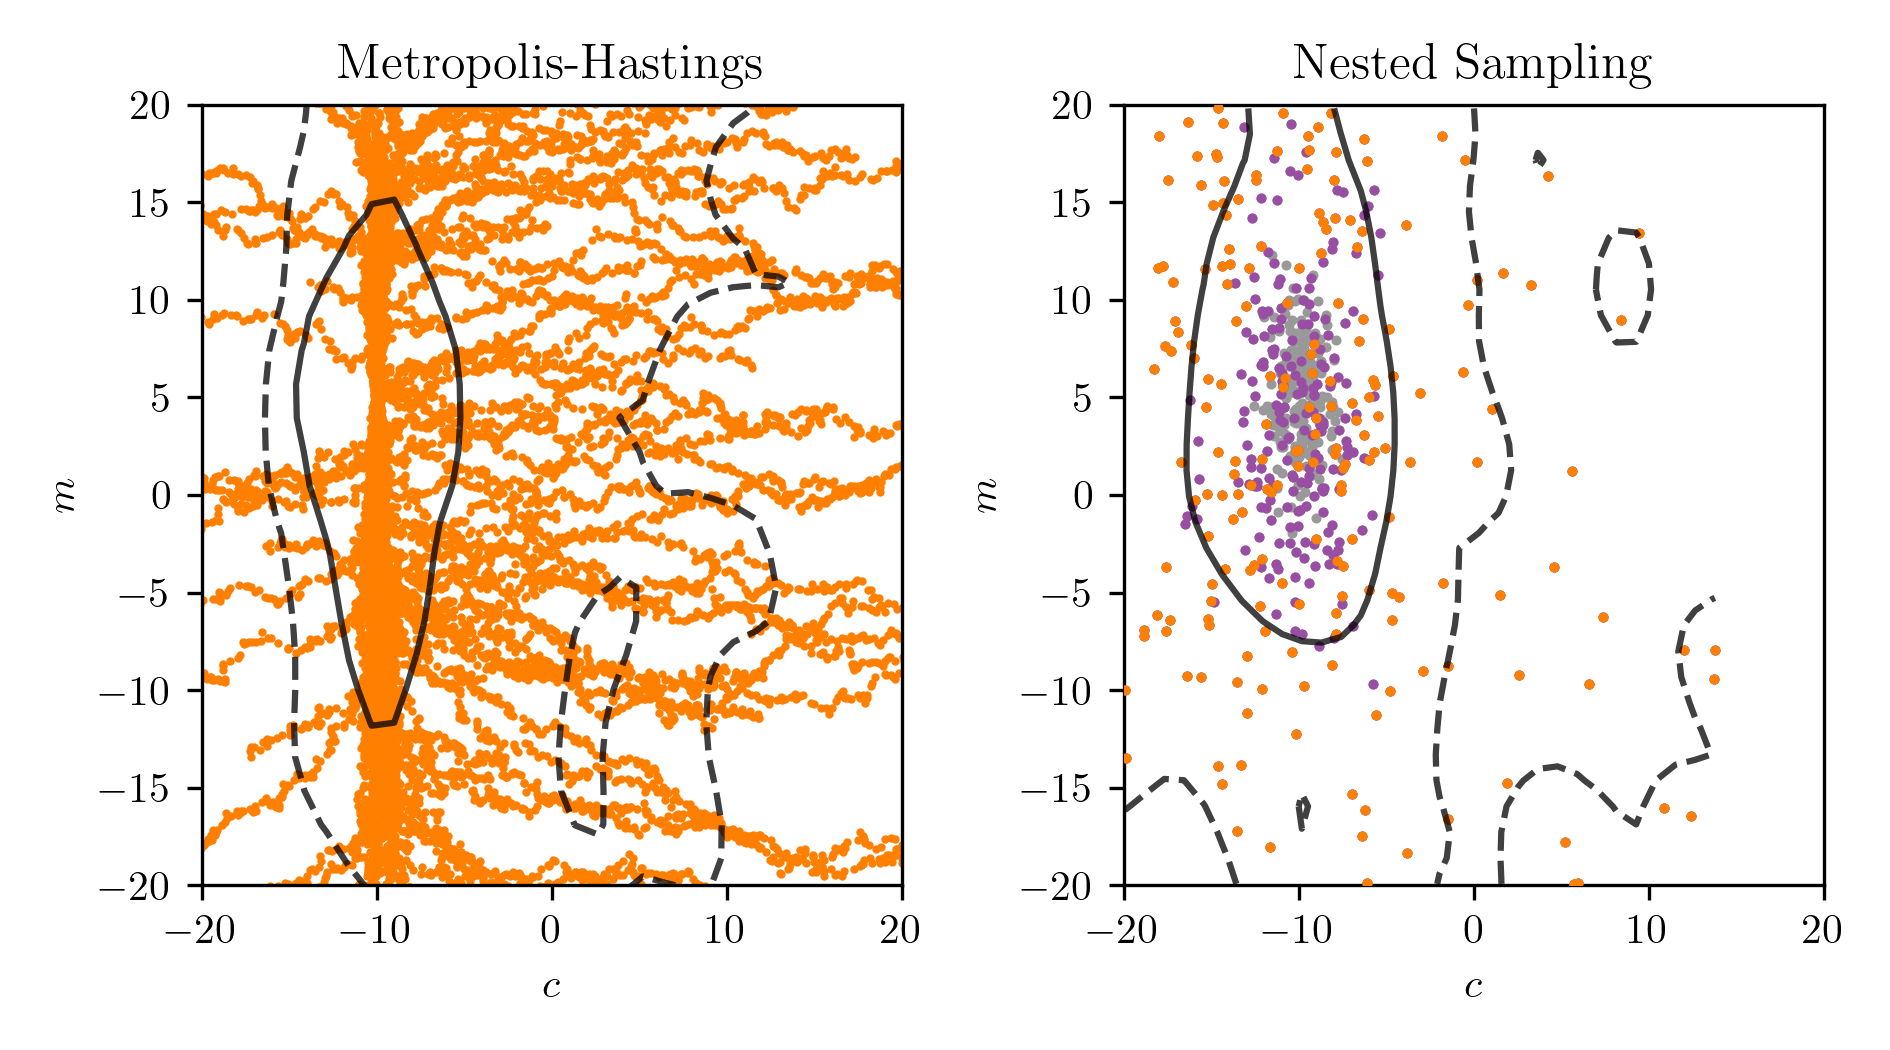
\includegraphics{introduction/figs/sampling_comparison.png}
    \caption{The figure shows a comparison of the random walk Metropolis-Hastings~(MH) sampling algorithm on the left and a rejection based Nested Sampling~(NS) algorithm on the right. The MH algorithm evolves 100 walkers for 250 steps each to explore the parameter space and the NS algorithm evolves 100 live points for 600 iterations. For more details see the text.}
    \label{fig:sampling_comparison}
\end{figure}

Bayesian inference is often performed with Markov Chain Monte Carlo~(MCMC) methods like the Metropolis-Hastings algorithm \cite{Hastings_MCMC_1970} and affine invariant ensemble samplers \cite{Foreman_Mackey_2013}. These approaches often produce unnormalised samples of the posterior and do not directly provide an estimate of the evidence.

A simple example of an MCMC sampler is the Metropolis-Hastings algorithm. In the left panel of \cref{fig:sampling_comparison} we show the resultant posterior found when fitting the gradient, $m$, and intercept, $c$, of a straight line given by
\begin{equation}
    y = mx + c + \epsilon,
\end{equation}
where $m = 5$ and $c=-10$ and the noise $\epsilon \sim \mathcal{N}(0, \sigma)$ is Gaussian distributed with a standard deviation of $\sigma = 0.5$.

The Metropolis-Hastings algorithm is a random walker algorithm that starts in some randomly chosen or carefully curated place, $x_0 = \{m_0, c_0\}$, often within some bounds, and subsequently gets perturbed in random directions. The direction of the perturbation is chosen based on some proposal distribution, which is equivalent to the prior. Here the proposal distribution of the next step, $x_{i+1}$, is given by a Gaussian centred around the previous step, $x_{i}$
\begin{equation}
    \pi(x_{i+1}|x_{i}) = \frac{1}{\sigma \sqrt{2\pi}}\exp\bigg(-\frac{1}{2}\frac{(x_{i+1} - x_{i})^2}{\sigma^2}\bigg),
\end{equation}
where we have set the standard deviation, $\sigma = 0.2$. At each iteration, the likelihood for the new point, $x_{i+1}$, is calculated, for example with \cref{eq:log_likelihood}, and compared to the equivalent value for $x_{i}$. The proposal or prior weighted ratio of the two likelihoods is taken
\begin{equation}
    \alpha = \frac{\mathcal{L}(x_{i+1}) \pi(x_{i+1})}{\mathcal{L}(x_{i})\pi(x_{i})},
\end{equation}
and compared to a random number, $u$, from a uniform distribution between $0 - 1$. If $u \leq \alpha$ then the new point is accepted into the chain else $x_{i}$ is perturbed again in a different random direction and the process is repeated. It is often more convenient to work in log-space because the likelihoods are very small, meaning that our inequality is given by
\begin{equation}
    \log_{10}(u) \leq \log_{10}(\alpha) = \log_{10}(\mathcal{L}(x_{i+1})) - \log_{10}(\mathcal{L}(x_{i})) + \log_{10}(\pi(x_{i+1})) - \log_{10}(\pi(x_{i})).
\end{equation}

The idea here is to climb up the likelihood contour but allow for occasional steps down the contours in an effort to prevent missing maxima in multi-modal problems. For example, in the case where the likelihood of step $x_{i+1}$ is higher than for step $x_{i}$ then $\alpha$ is always greater than 1 and always greater than $u$. However, if the likelihood for step $x_{i+1}$ is less than for $x_{i}$ then $\alpha < 1$ but if $u$ is randomly chosen to be less than $\alpha$ the step is accepted. This leads to a more complete exploration of the parameter space whilst maintaining a degree of efficiency and a focus on the maximum likelihood value. Through this process, the algorithm generates samples on the posterior distribution.

Here, the choice of $\sigma$ in the proposal distribution has a significant impact on how the algorithm converges. In fact, the functional form of the proposal distribution strongly impacts how the space is explored and the efficiency with which the maximum likelihood value is found. The samples from HERA used in \cref{ch:hera_saras3} were derived using ensemble MCMC techniques, where the new sample points are chosen based on the distribution of all the current live points or walkers \cite{Foreman_Mackey_2013, Ashton_ns_review_2022}.

In contrast, the Nested Sampling algorithm, used throughout this thesis, evolves a series of live points, $n_{\mathrm{live}}$, up the likelihood contour \cite{skilling_nested_2004, Ashton_ns_review_2022} in an effort to approximate the Bayesian evidence. The algorithm begins by evaluating the likelihood for the initial $n_{\mathrm{live}}$ points chosen from the prior distribution $\pi(\theta)$. The lowest likelihood point is then discarded and a new point is drawn from the prior with a higher likelihood than the discarded point. At each iteration the volume contained by the live points is compressed exponentially from an initial value of $X_0 = 1$, i.e. the prior, to $X_{i+1} = \exp(-1/n_\mathrm{live}) X_{i}$.% and the evidence is incremented by the product of the likelihood and $\Delta X / 2$. 

The evidence is therefore given by
\begin{equation}
    \mathcal{Z} = \sum^{n_\mathrm{iter}}_{i=1} w_i L^*_i
\end{equation}
where $L^*_i$ is the discarded likelihood at each iteration between $i=1$ and the total number of iterations $n_\mathrm{iter}$. The weights $w_i$ are given by
\begin{equation}
    w_i = \frac{1}{2}(X_{i+1} - X_{i-1}).
\end{equation}

The rejected sample at each iteration $i$ has an associated likelihood, weight, evidence and prior probability, which means that the Nested Sampling algorithm generates normalised samples on the posterior. We can then interpret this to tell us which parameter values in our prior ranges best describe the data.

Nested sampling is compared with the Metropolis Hastings algorithm in \cref{fig:sampling_comparison} using the same two-dimensional line fitting problem discussed previously.

The simplest sampling algorithm where a new sample is randomly drawn from the prior to replace the discarded point is slow, and alternatives such as slice sampling are much more efficient \cite{Neal_sampling_2000}. Slice sampling was originally implemented in a Nested Sampling algorithm in \cite{Aitken_sampling_2013} and extended in \cite{Handley2015a, Handley2015b} to work in higher dimensions. 

%In slice sampling we reject the lowest likelihood point, randomly select a point from the remaining live points and define a randomly chosen principle axis through that point. We then sample uniformly along a given length of that principle axis and if the likelihood of the new point is less than that of the rejected point we shrink the range along the axis that we are drawing samples from. The initial width of the slice is defined by the width of the likelihood contour, and the shrinking is designed to deal with multi-modal distributions. If the likelihood is larger, we pick another direction and repeat the process for a given number of repeats. We repeat the sampling to prevent the new point and the original point that we sliced through being correlated, and to be confident that the new point has been drawn from the prior.

Nested sampling algorithms typically rely on stopping criteria that determine the number of iterations to perform. It can become increasingly less rewarding to try to find replacement live points with higher likelihoods as you travel up the likelihood contours. A commonly used stopping criteria is when the fractional increase in the evidence is below some user specified tolerance
\begin{equation}
    \Delta \mathcal{Z}/Z < \mathrm{tol}.
\end{equation}

Bayesian inference techniques are well established in the field of cosmology and have been used for a number of years due to pioneering work analysing the CMB data~\cite{Trotta_bayes_2008}. However, it is only in the last few years, due to the increased interest in the field after the reported EDGES detection (see \cref{sec:current_results}), that Bayesian techniques have been applied to data from 21-cm cosmology experiments. 

For example, in an analysis of data from SARAS2 the authors used likelihood ratios, comparing fits with and without signal models, to rule out certain astrophysical scenarios for the global 21-cm signal \cite{Singh_saras2_2017}. The likelihood ratio is defined by
\begin{equation}
    \mathcal{R} = \frac{\mathcal{L}_{M, 1}}{\mathcal{L}_{M, 2}},
\end{equation}
and when its value is $> 1$ then model one is preferred over model two. While likelihood ratios give an intuitive means of determining whether one model is more probable relative to another, they are a \textit{relative} metric, unlike the Bayesian Evidence which is an absolute metric. Further, likelihood ratios do not appropriately account for the choice of prior, which the Bayesian Evidence does.

In an analysis of data from the EDGES high band instrument, the authors generated several million simulations of their data from a wide prior and calculated their corresponding likelihoods to estimate the posterior without using MCMC or Nested Sampling \cite{Monsalve_EDGES_HB_3_2019}. Finally, a significant number of experimental efforts have employed MCMC sampling to explore the astrophysical parameter space of the 21-cm power spectrum including LOFAR \cite{Ghara_LOFAR_2020} and MWA \cite{Ghara_MWA_2021}. 

Forward modelling of the global 21-cm signal in a Bayesian Nested Sampling pipeline has been pioneered by the REACH collaboration \cite{Anstey_REACH_2021, Anstey_antenna_2022}. Bayesian inference is employed significantly in this thesis, in which the Nested Sampling algorithm, implemented with \textsc{multinest} \cite{multinest_2008, multinest_2009, multinest_2019, PyMultiNest} and \textsc{polychord} \cite{Handley2015a, Handley2015b}, is used to model data from EDGES, LEDA, SARAS2, SARAS3, Planck, the Dark Energy Survey~(DES) and HERA.

\section{Machine learning and 21-cm Cosmology}
\label{sec:neural_networks}

Machine learning has many applications in the field of 21-cm cosmology. It has been shown that neural networks can capture the complex relationship between the 21-cm signal and the astrophysical process in the first billion years of cosmic history to a high degree of accuracy by \cite{Cohen2020} and more recently using two different approaches in \cite{Bevins_globalemu_2021} (\cref{ch:globalemu}) and \cite{21cmVAE}. The semi-numerical simulations that are used to model this signal take of order a few hours to produce per signal, whereas neural network emulators can produce estimates of these signals to varying degrees of accuracy in 10s of milliseconds. This is particularly important if we want to physically model signals in Bayesian Nested Sampling or MCMC runs where we are making thousands of calls to our signal generator, as in the latter half of this thesis.

In these scenarios, parameters, such as the star formation efficiency and virial circular velocity among others, are passed as inputs to a feed forward neural network and corresponding estimates of the 21-cm brightness temperature are output. An example network is shown in \cref{fig:neural_network}. In this example, the network takes two inputs, $p_1$ and $p_2$, and converts them to an output, $O_1$. Each node in the network is connected to all the nodes in the following layers, producing a `fully connected' feedforward network. When a numerical value is passed from one layer to the next, it is multiplied by the weight of the connection, $w_{ij}$ and a bias, $\beta_{ij}$ is added where $i$ corresponds to the node in the previous layer and $j$ the node in the next layer. For example, when $p_1$ is passed to the first node in the first layer, the value received is $w_{11} p_1 + \beta_{11}$. In addition, the node receives a weighted and shifted version of input $p_2$, since the network is fully connected, meaning that the value at node one (subscript) in layer one (superscript) is
\begin{equation}
    a_1^1 = w_{11} p_1 + w_{21} p_2 + \beta^1_1,
\end{equation}
where we define the bias at node one in layer one to be $\beta_1^1 = \beta_{11} + \beta_{21}$ or more generally $\beta_j^n =\sum_i \beta_{ij}$. The value at node one in layer one is scaled via an activation function into $a^{1 \prime}_1$. 

Activation functions can take many different forms and two examples, the sigmoid and linear, are shown in \cref{fig:neural_network}. The activation function is usually designed to introduce non-linearity in the network and allows the network to learn more complex relationships between the input and output. For this reason, the use of a linear output is often restricted to the final node and the sigmoid function is a common choice for the hidden layers, those between the input and output. $a^{1 \prime}_1$ is given by
\begin{equation}
    a^{1 \prime}_1 = \frac{1}{1+\exp(-a_{1}^1)}.
\end{equation}
$a^{1 \prime}_1$ is then passed to each node in the second layer and the process is repeated.

The number of layers and number of nodes in each layer is a choice for the user but can often be motivated by the demands of the problem as shown in \cref{ch:globalemu}. More complex structures in theory can model more complex relationships between the inputs and outputs of the network. However, arbitrarily increasing the size of the network can reduce the ability of the network to generalise to problems it has not seen before. This is a problem known as overfitting and is discussed in \cref{ch:globalemu} and \cite{Bevins_globalemu_2021}.

\begin{figure}[h!]
    \centering
    \begin{tikzpicture}[rednode/.style={circle, draw=red!60, fill=red!5, very thick, minimum size=5mm},
                bluenode/.style={circle, draw=blue!60, fill=blue!5, very thick, minimum size=5mm},
                greennode/.style={circle, draw=green!60, fill=green!5, very thick, minimum size=5mm},
                node distance=0.5cm and 2cm,
                remember picture]
        \node (0) {};
        \node[bluenode, above left=of 0, text width=0.5cm, align=center](input_1) {$p_1$};
        \node[bluenode, below left=of 0, text width=0.5cm, align=center](input_2) {$p_2$};

        \node[rednode, below right=of input_1, text width=0.5cm, align=center](layer1_center) {};
        \node[rednode, above=of layer1_center, text width=0.5cm, align=center](layer1_top) {};
        \node[rednode, below=of layer1_center, text width=0.5cm, align=center](layer1_bottom) {};

        \node[below=of layer1_bottom, inner sep=0pt] (sigmoid1) {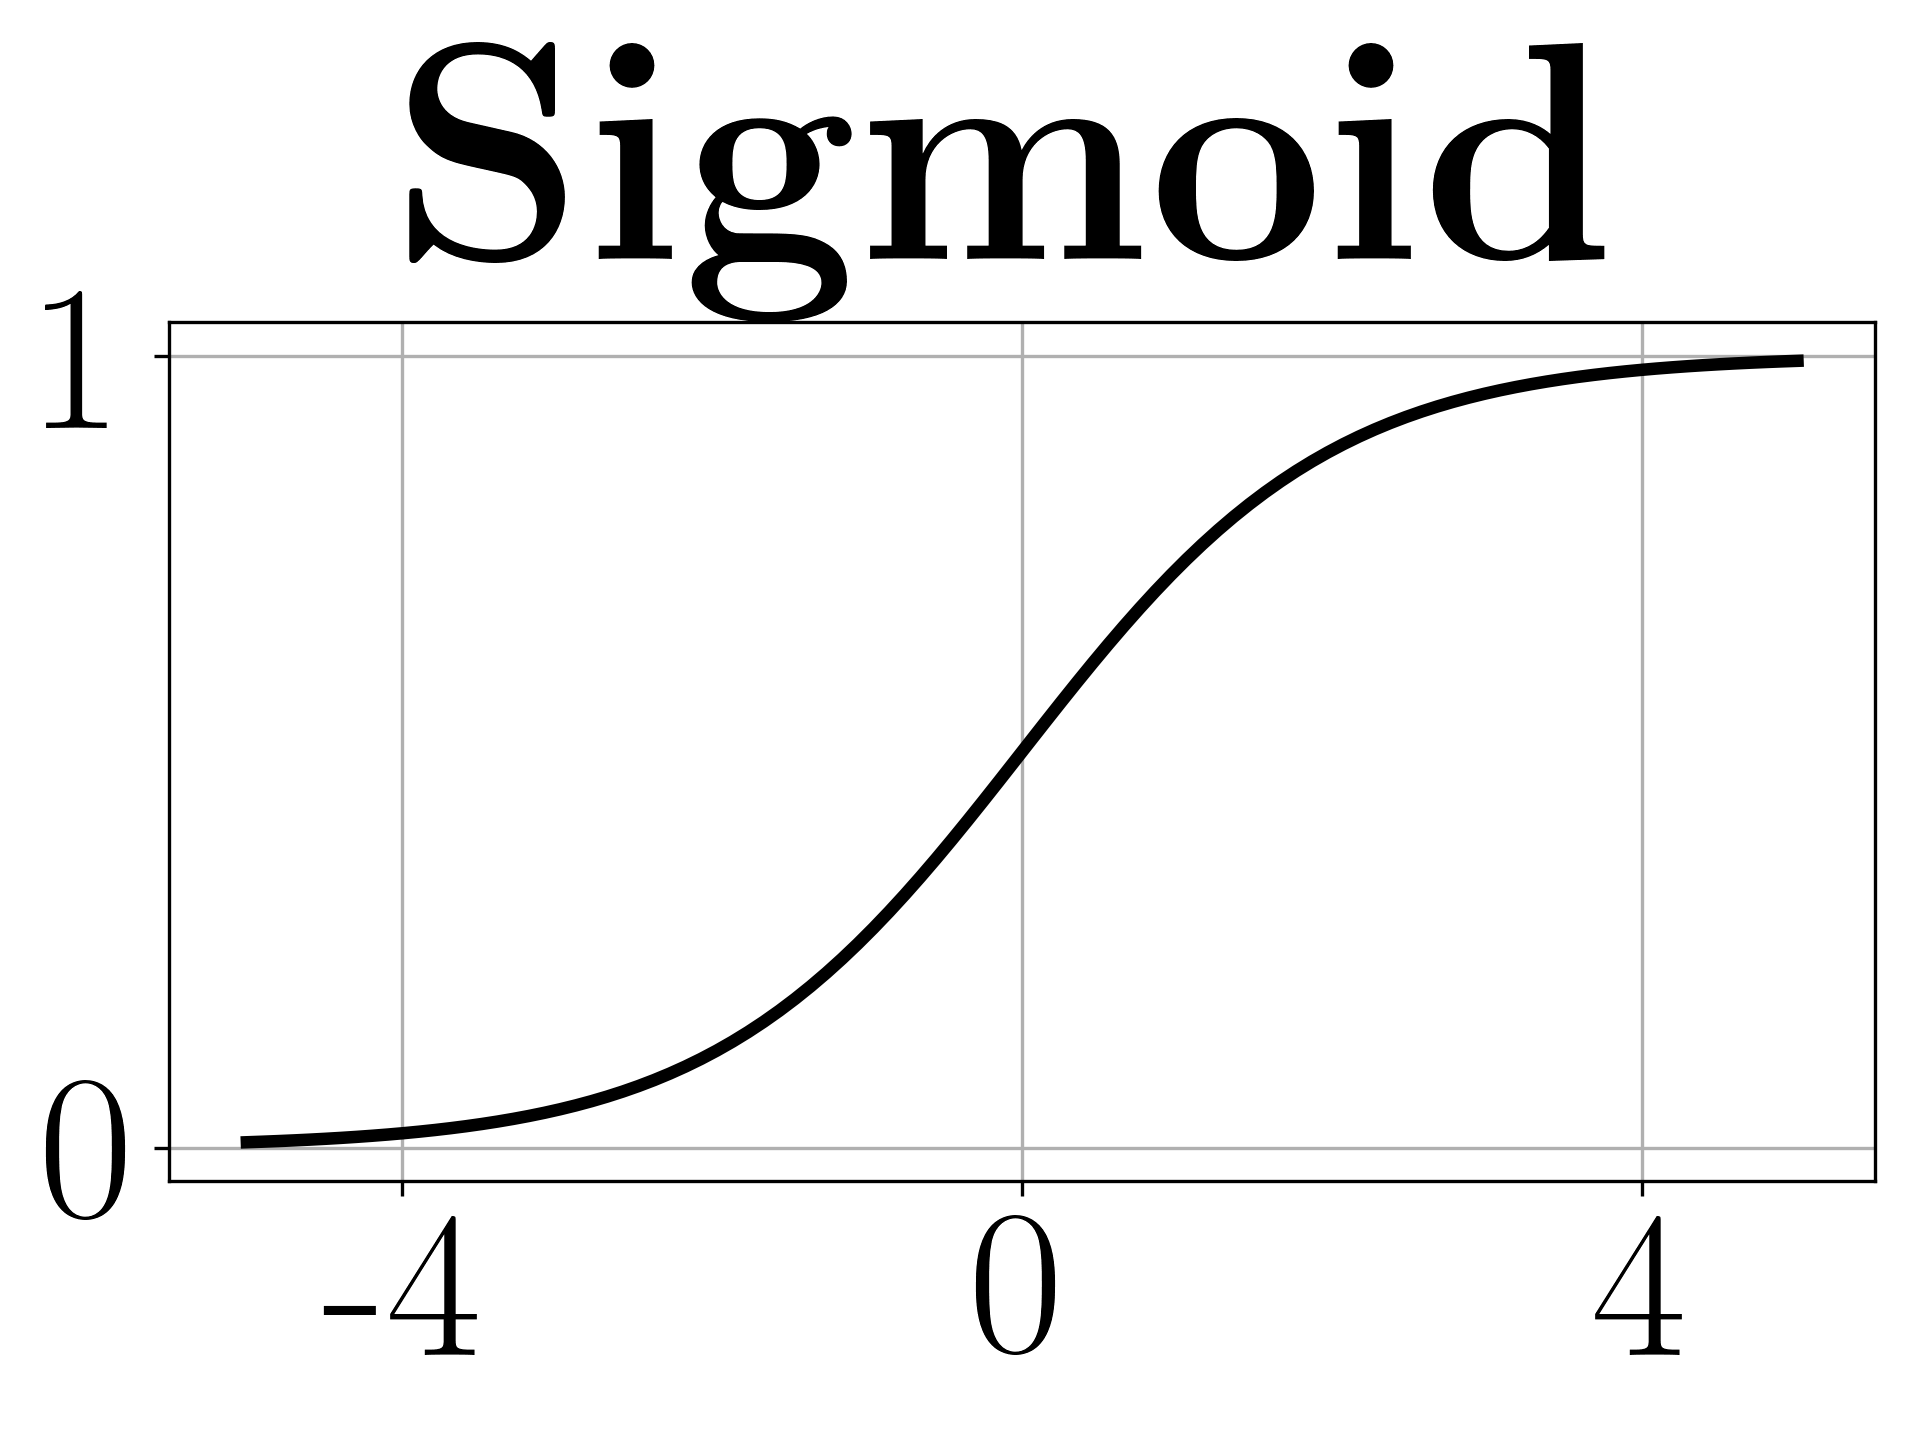
\includegraphics[width=.1\textwidth]{introduction/figs/sigmoid_function.png}};

        \node[rednode, right=of layer1_center, text width=0.5cm, align=center](layer2_center) {};
        \node[rednode, above=of layer2_center, text width=0.5cm, align=center](layer2_top) {};
        \node[rednode, below=of layer2_center, text width=0.5cm, align=center](layer2_bottom) {};

        \node[below=of layer2_bottom, inner sep=0pt] (sigmoid1) {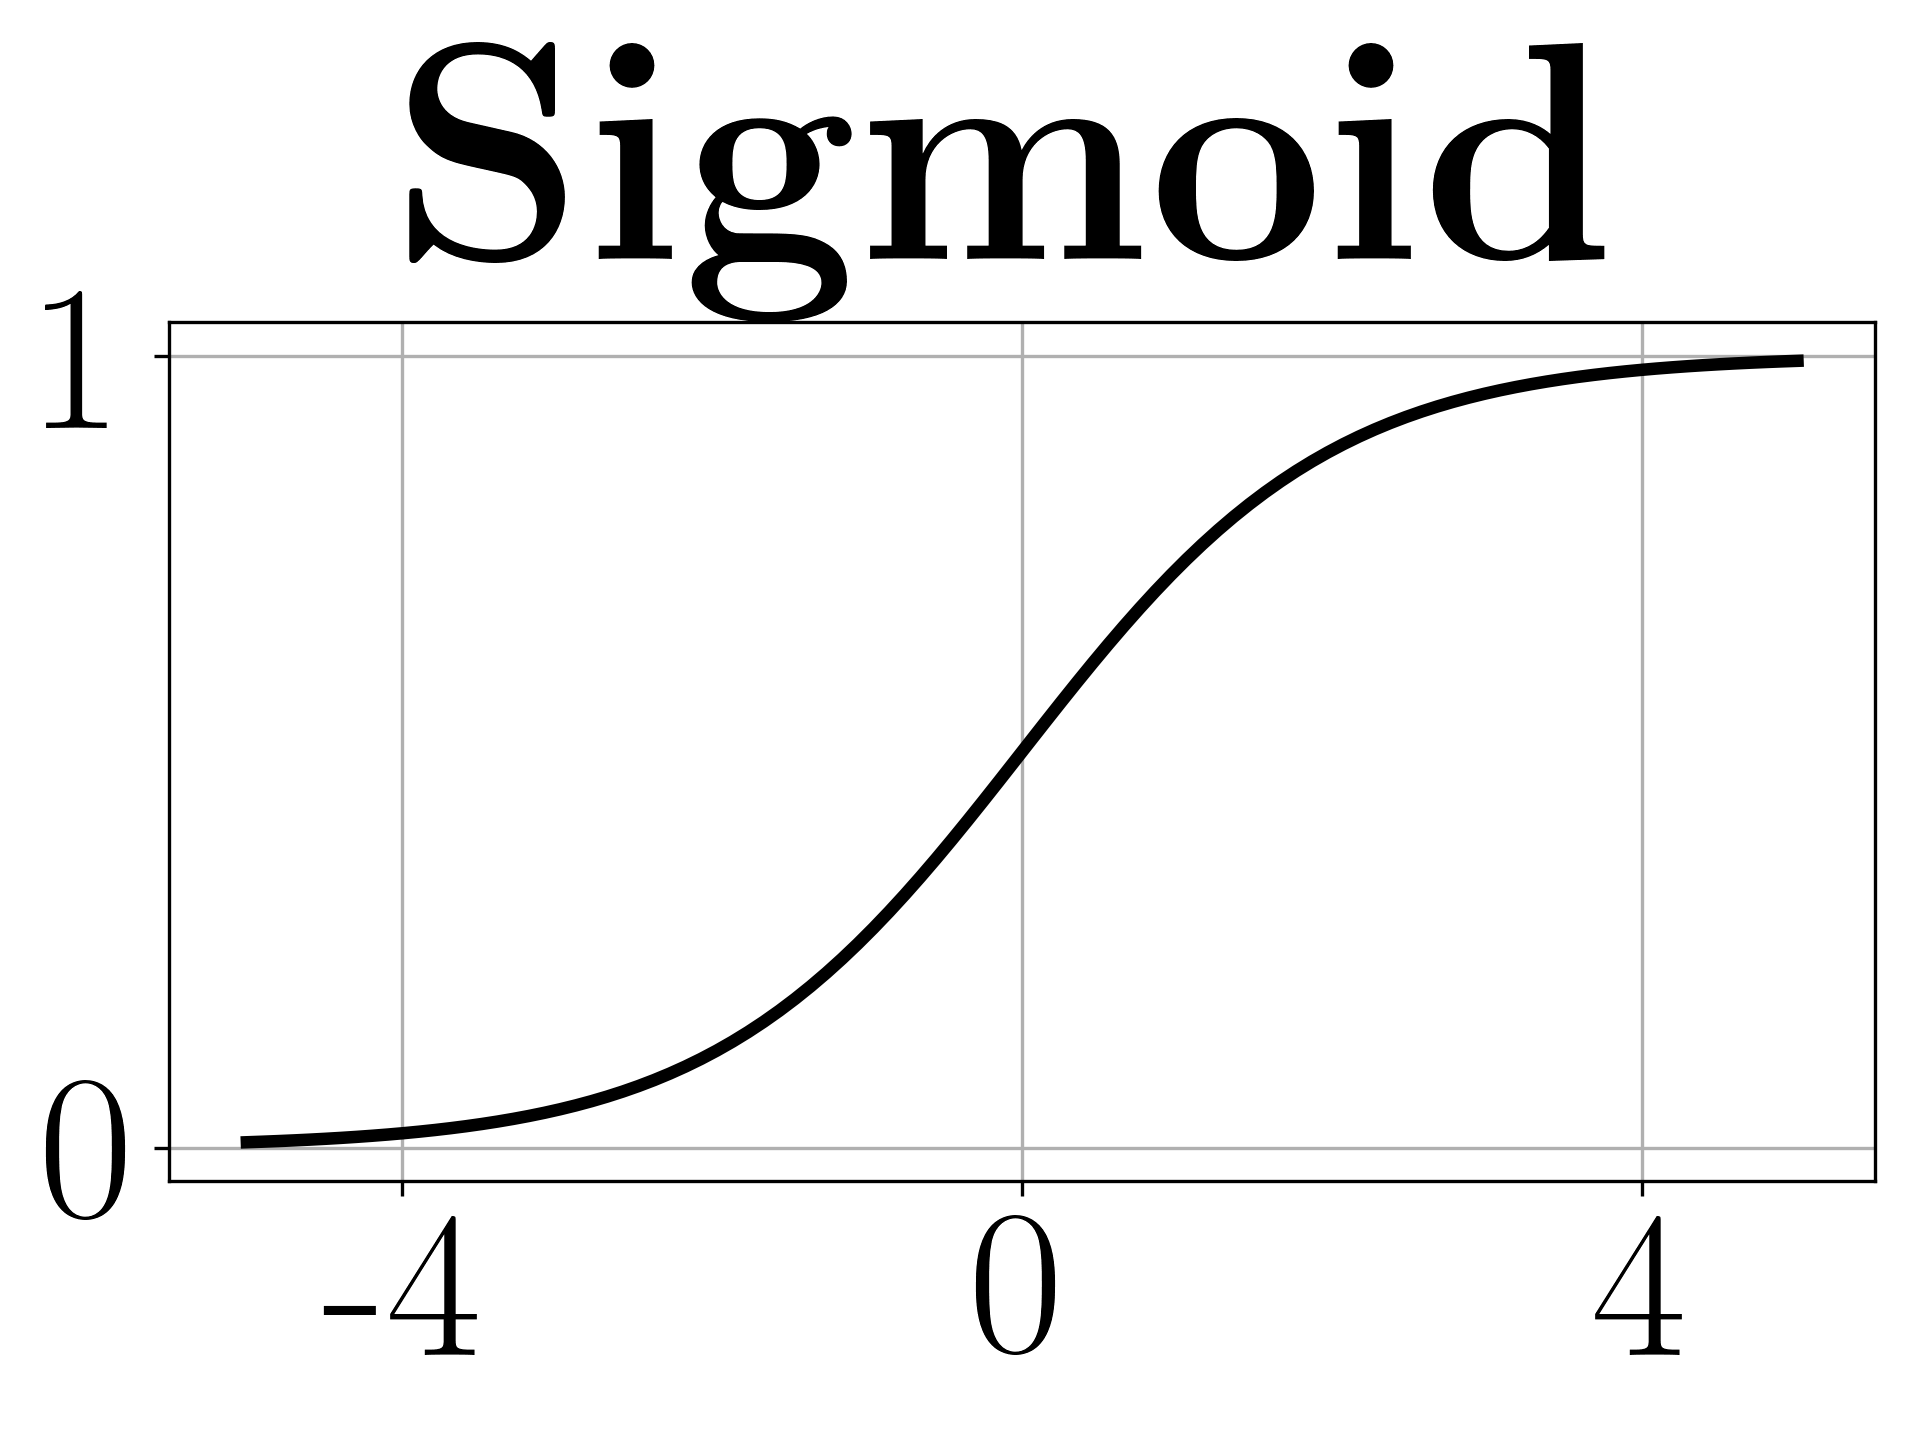
\includegraphics[width=.1\textwidth]{introduction/figs/sigmoid_function.png}};

        \node[greennode, right=of layer2_center, text width=0.5cm, align=center](output_1) {$O_1$};
        %\node[greennode, below right=of layer2_center, text width=0.5cm, align=center](output_2) {$O_2$};

        \node[below=of output_1, inner sep=0pt] (sigmoid1) {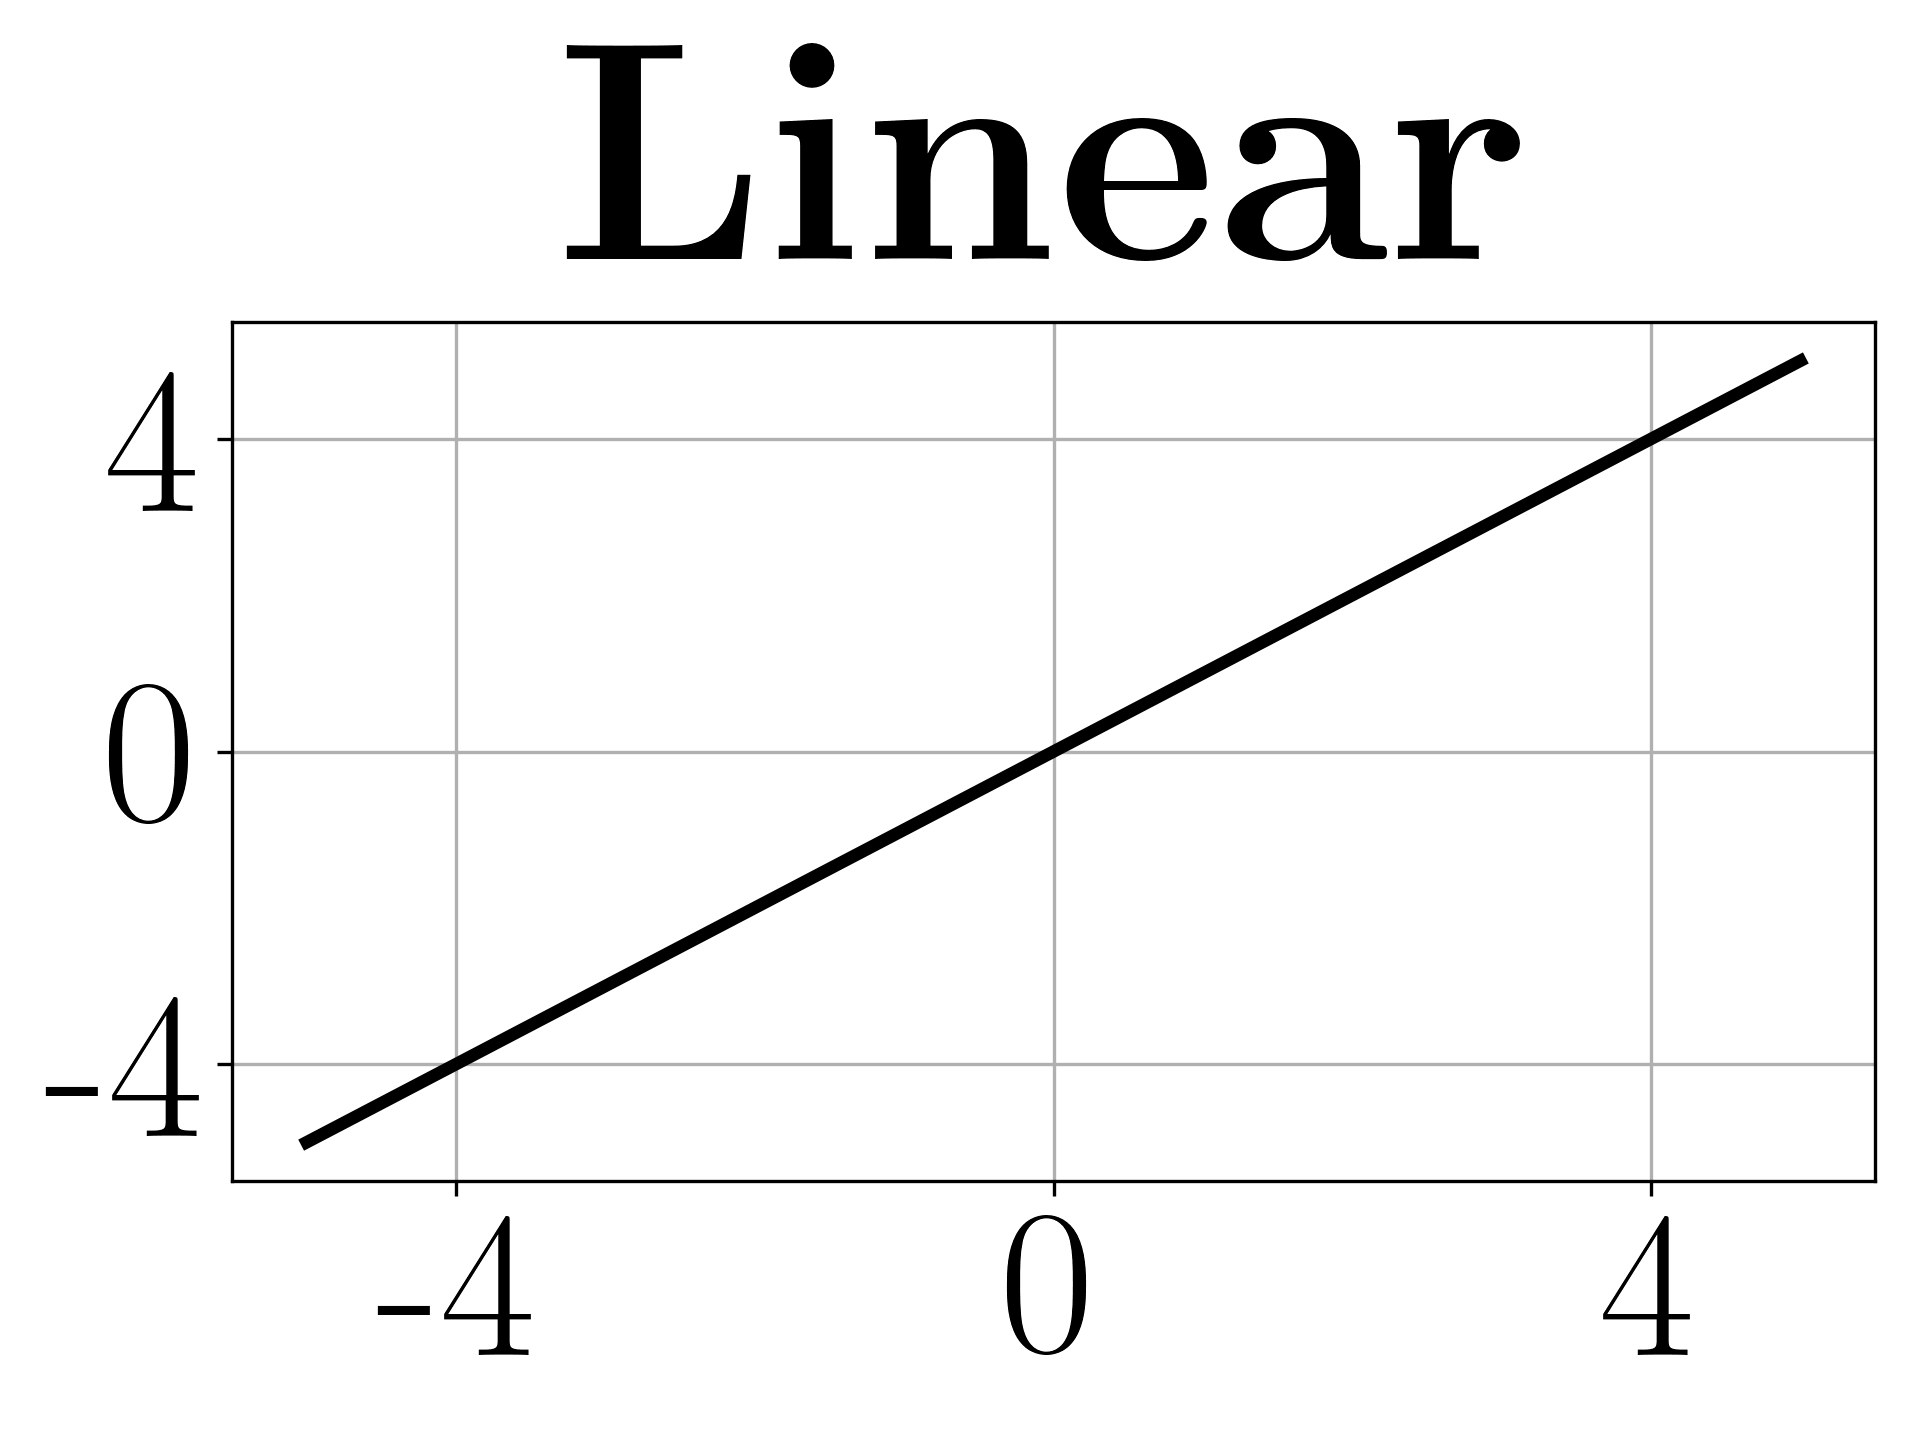
\includegraphics[width=.1\textwidth]{introduction/figs/linear_function.png}};

        \draw[->](input_1.east) -- (layer1_top.west) node[midway,above] {$w_{ij},~\beta_{ij}$};
        \draw[->](input_1.east) -- (layer1_bottom.west);
        \draw[->](input_1.east) -- (layer1_center.west);

        \draw[->](input_2.east) -- (layer1_top.west);
        \draw[->](input_2.east) -- (layer1_bottom.west);
        \draw[->](input_2.east) -- (layer1_center.west);

        \draw[->](layer1_bottom.east) -- (layer2_top.west);
        \draw[->](layer1_bottom.east) -- (layer2_center.west);
        \draw[->](layer1_bottom.east) -- (layer2_bottom.west);

        \draw[->](layer1_center.east) -- (layer2_top.west);
        \draw[->](layer1_center.east) -- (layer2_center.west);
        \draw[->](layer1_center.east) -- (layer2_bottom.west);

        \draw[->](layer1_top.east) -- (layer2_top.west) node[midway,above] {$w_{ij},~\beta_{ij}$};
        \draw[->](layer1_top.east) -- (layer2_center.west);
        \draw[->](layer1_top.east) -- (layer2_bottom.west);

        \draw[->](layer2_bottom.east) -- (output_1.west);

        \draw[->](layer2_center.east) -- (output_1.west);

        \draw[->](layer2_top.east) -- (output_1.west) node[midway,above right] {$w_{ij},~\beta_{ij}$};
    \end{tikzpicture}
    \caption{The diagram shows a simple feed forward neural network that takes two input parameters, $p_1$ and $p_2$, and transforms that to an output, $O_1$. $w_{ij}$ and $\beta_{ij}$ represent the weights and biases between layer $i$ and layer $j$. The diagrams at the bottom of the figure show two different activation functions which in the hidden layers of the network, those between the input and output, are designed to introduce non-linear structure into the model.}
    \label{fig:neural_network}
\end{figure}

The issue is therefore how to set the weights and biases of the neural network. These have to be learned based on some training data that we give to the network, i.e. a set of inputs and corresponding outputs, and a loss function. The loss function is chosen by the user, but typically we use a root mean squared error (or RMSE) loss given by
\begin{equation}
    \sigma_{NN} = \sqrt{\frac{1}{N}\sum (y_\mathrm{true}-y_\mathrm{pred})^2},
    \label{eq:loss_intro}
\end{equation}
where $y_\mathrm{true}$ is the true value of the output and $y_\mathrm{pred}$ is what the network predicts.

In \cref{eq:loss_intro}, $y_\mathrm{pred}$ is a function of the weights and biases of the network, and therefore we can say the same of the loss function, $\sigma_{NN}(\mathbf{w}, \mathbf{\beta})$. In order to optimize the values of the weights and biases, we minimise the loss function using a gradient descent algorithm, where at iteration $i+1$ the weights are updated according to
\begin{equation}
    \mathbf{w}_{i+1} = \mathbf{w}_i - \gamma \nabla \sigma(\mathbf{w}_i, \mathbf{\beta}_i),
\end{equation}
where $\gamma$ is known as the learning rate and determines the size of the step taken in the parameter space. The gradient effectively tells us which connections in the network have the largest impact on the loss. To evaluate the negative gradient of the loss function with respect to the weights and biases, we use the backpropagation algorithm.

The backpropagation algorithm begins by looking at how the weights and biases between the output and the previous layer need to change to improve the loss function for a particular example. To calculate the gradient of the loss with respect to each weight and bias between the output and the previous layer in the above example, we rely on the chain rule
\begin{equation}
    \frac{\delta \sigma}{\delta w^2_{ij}} = \frac{\delta \sigma}{\delta O_1} \frac{\delta O_1}{d w^2_{ij}}.
\end{equation}
For intermediate layers between the output and input there is an additional term accounting for the impact of the activation function. Since the output activation, the loss and the hidden layer nodes are known functions, we can use Automatic Differentiation to calculate their derivatives with respect to each weight and bias. Once we have expressions for all the derivatives, the algorithm updates the weights according to
\begin{equation}
    w^2_{ij} - \gamma \frac{\delta \sigma}{\delta w^2_{ij}}.
\end{equation}
starting with the weights between the input and the first hidden layer and propagating the change forward.
%The process, then propagates back through the network using the modified weights and biases between the output and the previous layer until all the weights and biases have been adjusted appropriately.
The algorithm calculates the required changes in the weights and biases for a series of training examples, and then averages the changes over many examples to try to improve the accuracy of the network while maintaining the ability for it to generalise to unseen test examples. 

We could do this for all examples in our training data and perform a gradient descent. However, this is a very computationally expensive task. For example, the network shown in \cref{fig:neural_network} has 18 weights and biases creating a 36 dimensional space to optimize and consequently training neural networks is non-trivial and there are many tricks that can be employed to try and improve their accuracy. Some of these are discussed in \cref{ch:globalemu}. However, the most basic trick typically employed is to divide the training data into batches and perform a stochastic gradient descent. The algorithm picks the most appropriate direction to move each weight and bias, and determines by how much to move them to improve the loss function for a specific subset of randomly chosen training examples. Doing this over many iterations for many batches, while sometimes increasing the loss for the whole training data set, eventually finds a good approximation to the true minimum or a local minimum that sufficiently optimizes the network and is much more computationally efficient than a full gradient descent. %The algorithm effectively up weights the most important inputs, or features, with respect to the output while allowing it to perform well on unseen data.

The neural network emulator \textsc{globalemu} discussed in \cref{ch:globalemu} is a typically small feed forward network. The previous state of the art global 21-cm signal emulator \textsc{21cmGEM} relies on several such networks and a decision tree \cite{Cohen2020}. The recently published \textsc{21cmVAE} relies on a Variational Autoencoder to compress the input parameter space into a lower dimensional latent space in which to learn the relationship with the output 21-cm signal \cite{21cmVAE}.  \textsc{globalemu} and \textsc{21cmVAE} represent the `next generation' emulators and the latter is more accurate but around 40 times slower than \textsc{globalemu}. Both emulators and \textsc{21cmGEM} are sufficiently accurate for the current noise levels in present experimental efforts. Recently, some of the techniques used in the development of \textsc{globalemu} have been applied to the emulation of the 21-cm power spectrum in the HERA analysis \cite{HERA_2022c}. %In global 21-cm cosmology the inverse problem, where the raw data is input and astrophysical parameters are output, is also possible and has been previously attempted \cite{Choudhury_2021}.

In \cref{ch:margarine}, we discuss a different type of machine learning algorithm known as a Masked Autoregressive Flow~(MAFs). MAFs are a form of normalising flow that string together a series of Masked Autoencoder for Distribution Estimation~(MADE) \cite{Germain_MADE_2015} networks to perform density estimation. They are an example of a Neural Density Estimator. Normalising flows allow us to calculate the log-probability, $\log(P(x))$, for a set of samples $\{x\}$ on some complex distribution. We assume that the multidimensional distribution $P(x)$ can be decomposed into a set of one-dimensional conditional distributions
\begin{equation}
P(x) = \prod_i P(x_i| x_1, x_2, ..., x_{i-1}),
\end{equation}
where the index $i$ represents the dimension. We model each conditional probability as a Gaussian distribution and assume a base standard normal distribution, $\mathcal{N}(0, 1)$, that is shifted and scaled by some standard deviation, $\sigma_i$, and mean, $\mu_i$, which can be written as
\begin{equation}
P(x_i| x_1, x_2, ..., x_{i-1}) = \mathcal{N}(\mu_i(x_1, x_2, ..., x_{i-1}), \sigma_i(x_1, x_2, ..., x_{i-1})),
\end{equation}
or alternatively written in terms of samples in $x_i$
\begin{equation}
x_i = \sigma_i z_i + \mu_i,
\end{equation}
where $z_i \sim \mathcal{N}(0, 1)$. The problem is how to estimate the appropriate set of $\sigma_i$ and $\mu_i$ to model the distribution of $x_i$. We do this with the MADE architecture which is shown in \cref{fig:maf} (see also \cite{Alsing2019}) and the change of variables principle
\begin{equation}
    P(x) = P(z) \bigg|\frac{\delta z}{\delta x}\bigg|
\end{equation}
which describes how one probability distribution can be transformed into another. Here the magnitude of the determinant of the Jacobian represents the change in volume between $P(x)$ and $P(z)$ and it ensures that $P(x)$ is normalised hence `normalising' flows.

\begin{figure}[h!]
    \centering
    \begin{tikzpicture}[rednode/.style={circle, draw=red!60, fill=red!5, very thick, minimum size=5mm},
                bluenode/.style={circle, draw=blue!60, fill=blue!5, very thick, minimum size=5mm},
                greennode/.style={circle, draw=green!60, fill=green!5, very thick, minimum size=5mm},
                node distance=0.5cm and 2cm,
                remember picture]
        \node (0) {};
        
        \node[rednode, above=of 0, text width=0.5cm, align=center](layer1_center1) {$\mu_2$};
        \node[rednode, below=of layer1_center1, text width=0.5cm, align=center](layer1_center2) {$\sigma_2$};
        \node[rednode, above=of layer1_center1, text width=0.5cm, align=center](layer1_top2) {$\sigma_1$};
        \node[rednode, above=of layer1_top2, text width=0.5cm, align=center](layer1_top1) {$\mu_1$};
        \node[rednode, below=of layer1_center2, text width=0.5cm, align=center](layer1_bottom1) {$\mu_3$};
        \node[rednode, below=of layer1_bottom1, text width=0.5cm, align=center](layer1_bottom2) {$\sigma_3$};
    
        \node[rednode, left=of layer1_top2, text width=0.5cm, align=center](hl1) {};
        \node[rednode, left=of layer1_center1, text width=0.5cm, align=center](hl2) {};
        \node[rednode, left=of layer1_center2, text width=0.5cm, align=center](hl3) {};
        \node[rednode, left=of layer1_bottom1, text width=0.5cm, align=center](hl4) {};
        
        \node[below=of hl4, inner sep=0pt] (tanh) {\includegraphics[width=.1\textwidth]{introduction/figs/tanh_function.png}};
        
        \node[bluenode, below left=of hl2, text width=0.5cm, align=center, yshift=0.3cm](input_2) {$x_2$};
        \node[bluenode, above=of input_2, text width=0.5cm, align=center, yshift=0.12cm](input_1) {$x_1$};
        \node[bluenode, below=of input_2, text width=0.5cm, align=center, yshift=0.1cm](input_3) {$x_3$};

        \node[greennode, right=of 0, text width=0.5cm, align=center, yshift=0.3cm](output_2) {$z^\prime_2$};
        \node[greennode, above=of output_2, text width=0.5cm, align=center, yshift=0.12cm](output_1) {$z^\prime_1$};
        \node[greennode, below=of output_2, text width=0.5cm, align=center, yshift=0.1cm](output_3) {$z^\prime_3$};
        
        \node[right=of output_2, align=left, xshift=-1.5cm, yshift=0.12cm] {$= (x_2 -\mu_2) / \sigma_2$};
        
        \node[right=of output_1, align=left, xshift=-1.5cm, yshift=0.12cm] {$= (x_1 -\mu_1) / \sigma_1$};
        
        \node[right=of output_3, align=left, xshift=-1.5cm, yshift=0.12cm] {$= (x_3 -\mu_3) / \sigma_3$};
        
        \draw[densely dashed](input_1.east) -- (output_1.west);
        
        \draw[densely dashed](input_2.east) -- (output_2.west);
        
        \draw[densely dashed](input_3.east) -- (output_3.west);
        
        \draw[->](input_1.east) -- (hl1.west);
        \draw[->](input_1.east) -- (hl2.west);
        \draw[->](input_1.east) -- (hl3.west);
        \draw[->](input_1.east) -- (hl4.west);
        
        %\draw[->](input_2.east) -- (hl1.west);
        %\draw[->](input_2.east) -- (hl2.west);
        \draw[->](input_2.east) -- (hl3.west);
        \draw[->](input_2.east) -- (hl4.west);
        
        %\draw[->](input_3.east) -- (hl1.west);
        %\draw[->](input_3.east) -- (hl2.west);
        %\draw[->](input_3.east) -- (hl3.west);
        %\draw[->](input_3.east) -- (hl4.west);
        
        \draw[->](hl1.east) -- (layer1_center1.west);
        \draw[->](hl2.east) -- (layer1_center1.west);
        %\draw[->](hl3.east) -- (layer1_center1.west);
        %\draw[->](hl4.east) -- (layer1_center1.west);
        
        \draw[->](hl1.east) -- (layer1_center2.west);
        \draw[->](hl2.east) -- (layer1_center2.west);
        %\draw[->](hl3.east) -- (layer1_center2.west);
        %\draw[->](hl4.east) -- (layer1_center2.west);
        
        %\draw[->](hl1.east) -- (layer1_top1.west);
        %\draw[->](hl2.east) -- (layer1_top1.west);
        %\draw[->](hl3.east) -- (layer1_top1.west);
        %\draw[->](hl4.east) -- (layer1_top1.west);
        
        %\draw[->](hl1.east) -- (layer1_top2.west);
        %\draw[->](hl2.east) -- (layer1_top2.west);
        %\draw[->](hl3.east) -- (layer1_top2.west);
        %\draw[->](hl4.east) -- (layer1_top2.west);
        
        \draw[->](hl1.east) -- (layer1_bottom2.west);
        \draw[->](hl2.east) -- (layer1_bottom2.west);
        \draw[->](hl3.east) -- (layer1_bottom2.west);
        \draw[->](hl4.east) -- (layer1_bottom2.west);
        
        \draw[->](hl1.east) -- (layer1_bottom1.west);
        \draw[->](hl2.east) -- (layer1_bottom1.west);
        \draw[->](hl3.east) -- (layer1_bottom1.west);
        \draw[->](hl4.east) -- (layer1_bottom1.west);
        
        \draw[densely dashed](layer1_top1.east) -- (output_1.west);
        \draw[densely dashed](layer1_top2.east) -- (output_1.west);
        
        \draw[densely dashed](layer1_center1.east) -- (output_2.west);
        \draw[densely dashed](layer1_center2.east) -- (output_2.west);
        
        \draw[densely dashed](layer1_bottom1.east) -- (output_3.west);
        \draw[densely dashed](layer1_bottom2.east) -- (output_3.west);

    \end{tikzpicture}
    \caption{The MADE architecture, when trained appropriately, transforms samples from a complex probability distribution $\{x\}$ on to samples from a standard normal distribution under the assumption that the probability distribution $\{x\}$ can be broken into conditional one-dimensional probability distributions represented as Gaussians. Many different MADE networks can be stacked together and trained to produce a normalising flow increasing the expressivity of the density estimation. By definition normalising flows are bijective, and a trained implementation can be used to calculate $\log(P(x))$ and draw samples from $P(x)$.}
    \label{fig:maf}
\end{figure}

The MADE architecture takes in sets of samples from $\{x\}$ and estimates the value of $\mu_i$ and $\sigma_i$ needed to transform them to samples on the standard normal distribution $\{z\}$. Doing this for many sets of samples in $\{x\}$ adjusts the networks weights and biases appropriately to transform the distribution as a whole. The base of the MADE architecture is a fully connected neural network like that in \cref{fig:neural_network} however certain connections are masked out to represent the fact that probability distributions and hence $\mu_i$ and $\sigma_i$ are conditional on samples from $x_{i-1}$ dimensions. The masking is performed by multiplying the matrices of associated weights with a binary mask.

$\sigma_i$ and $\mu_i$ are functions of the weights and biases in the MADE network, which can have multiple hidden layers with varying activation functions.%, and the idea is to minimise the loss function
%\begin{equation}
%    \mathrm{min}(\log(P(z^\prime)) + \log(\bigg|\frac{\delta z^\prime}{\delta x}\bigg|)),
%\end{equation}
%where here the change of variables is from the true standard normal distribution to the output of the neural network $z^\prime_i = (x_i - \mu_i)/\sigma_i$ which should, subject to appropriately chosen $\mu_i$ and $\sigma_i$, look identical. By minimising the above we are minimising the volume contraction between the output samples and the expected standard normal distribution thus generating an invertible transformation from the standard normal to  our target distribution $\{x\}$. 
The idea is to minimize the Kullback-Leibler~(KL) divergence between the true probability distribution of the samples $x$ and the prediction from the network $P_\theta(x)$ given by
\begin{equation}
    \mathcal{D} (P(x)||P_{\theta}(x)) = -\mathbb{E}_{P(x)}[\log P_\theta(x)] + \mathbb{E}_{P(x)}[\log P(x)],
\end{equation}
where $\theta$ represents the hyperparameters of the network. The second term in the KL divergence is independent of the network and so for a minimization problem we can ignore this and
\begin{equation}
    -\mathbb{E}_{P(x)}[\log P_\theta(x)] = -\frac{1}{N} \sum_{1=0}^N \log P_\theta(x_i),
\end{equation}
meaning that our minimization problem becomes
\begin{equation}
    \argmax_\theta \sum^N_{i=0} \log P_\theta(x_i),
\end{equation}
or equivalently by a change of variables
\begin{equation}
    \argmax_\theta \sum_{i=0}^N [\log P_\theta(z_i^\prime) + \log \bigg|\frac{\delta z_i^\prime}{\delta x_i}\bigg|],
\end{equation}
where $z^\prime$ is a function of $\theta$ \cite{Alsing2019}. Here the second term is just the derivative over the network and the first term is trivially calculated from the output $\sigma$ and $\mu$.

We can stack many such networks together and train them in unison to transform more complicated networks under the following
\begin{equation}
    \begin{split}
    \mathbf{z}_0 & = \mathcal{N}(0, 1) \\
    \mathbf{z}_1 & = \mathbf{z}_0 \boldsymbol{\sigma}_1(\mathbf{z}_0, \mathbf{w}) + \boldsymbol{\mu}_1(\mathbf{z}_0, \mathbf{w})\\
    \vdots &\\
    \mathbf{x} & = \mathbf{z}_{n-1} \boldsymbol{\sigma}_n(\mathbf{z}_{n-1}, \mathbf{w}) + \boldsymbol{\mu}_n(\mathbf{z}_{n-1}, \mathbf{w}),
    \end{split}
\label{eq:MAF}
\end{equation}
in a normalising flow. Here $\mu_j$ and $\sigma_j$ are $N$-dimensional vectors, $\mathbf{z}_0$ is our multidimensional standard normal distribution and $\mathbf{x}$ is the multidimensional target distribution. The intermittent $\mathbf{z}_j$ distributions are output from one MADE and passed to the next and the weights and biases are adjusted across the whole chain at each training step. The transformation performed by a normalising flow is bijective in that there is a one-to-one relationship between samples in the base distribution and the target distribution, so we can go back and forth between the two passing the emulator samples on the standard normal distribution and recovering samples on the input posterior for example. Normalising flows and MAFs have many applications which are discussed in \cref{ch:margarine}.

There are many additional applications of machine learning in the field of 21-cm cosmology such as the use of Convolutional Neural Networks to accurately emulate tomographic images of the 21-cm field and modelling foregrounds in power spectrum analysis. However, we refer the reader to the literature for more details as the focus of this thesis is primarily on the global 21-cm signal.

\section{Current experimental results}
\label{sec:current_results}

The 21-cm line from neutral hydrogen has long been understood to be a powerful probe of galactic physics \cite{Furlanetto_review_2006, Barkana_review_2016, Mesinger2019}. However, it is only in the past 20-30 years that its potential usefulness as a cosmological probe has really been explored (see the historical review in \cite{Furlanetto_review_2006}). Making tomographic images of the 21-cm signal as a function of redshift was first proposed in \cite{Madau1997} and is a target of the upcoming Square Kilometre Array~(SKA) \cite{Mellema_SKA_2013}.

To date, observational efforts have focused on two different but related statistics known as the 21-cm power spectrum and global or sky-averaged 21-cm signal. Detection of the 21-cm power spectrum has been attempted by a number of different telescopes including LOFAR \citep[LOw-Frequency ARray,][]{LOFAR_current_EoR_2018, Gehlot_lofar_2019, Ghara_LOFAR_2020, Mondal_LOFAR_2020, Greig_LOFAR_2021}, MWA \citep[Murchison Widefield Array,][]{Trott_mwa_2020, Greig_MWA_2020, Ghara_MWA_2021}, HERA \cite{HERA_2017, HERA_2022b} and GMRT \citep[Giant Metrewave Radio Telescope,][]{GMRT2011}. However, current observations are limited by our understanding of the systematics in the data.

The global 21-cm signal is in principle easier to detect than the power spectrum. Observations were first proposed in \cite{Shaver1999} and a number of ongoing experimental efforts are underway to detect this signal. While the detection of the power spectrum requires the use of an interferometer to measure the temperature variation across different angular scales on the sky, the global 21-cm signal can be detected, in principle, with a single antenna. A number of different experiments have attempted to make detections, are currently underway or have been proposed to make this measurement, including EDGES \cite{Bowman_edges_2018, EDGES_high_band_experimental_paper_2017}, SARAS \cite{SARAS2_radiometer_2018, SARAS_reciever_2021, SARAS3_antenna_2021, SARAS3_spectrometer_2020}, LEDA \cite{Price_LEDA_2018}, SCI-HI \citep[Sonda Cosmol\'{o}gica de las Islas para la Detecci\'{o}n de Hidr\'{o}geno Neutro,][]{SCIHI}, BIGHORNS \citep[Broadband Instrument for Global HydrOgen ReioNisation Signal,][]{BIGHORNS}, PRIZM \cite{Philip_PRIZM_2019}, MIST \citep[Mapper of the IGM Spin Temperature,][]{MIST}, FARSIDE \citep[Farside Array for Radio Science Investigations of the Dark ages and Exoplanets,][]{Burns_Moon_2021}, and REACH \cite{Acedo_REACH_2019, Anstey_REACH_2021,Cumner_antenna_2021, Anstey_antenna_2022, de_lera_acedo_reach_2022}.

In the following subsections, we explain the state of the field up to 2019, the start of this PhD, with some reference to more recent experimental results such as SARAS3 and HERA which are explored more in the main text. Part III of this thesis and the corresponding chapters detail improvements to our current understanding of the early Universe that I have been responsible for leading.

\subsection{The sky-averaged 21-cm signal}

A tentative detection of the global 21-cm signal was reported by the EDGES collaboration in 2018 \cite{Bowman_edges_2018}. If true, the detection implies rapid star formation, delayed and then rapid X-ray heating, an earlier than expected end to the epoch of reionization and exotic astrophysics such as an increased radio background \cite{FengRB2018, JanaRB2018, EwallRB2018, MirochaRB2019, Reis2020} or interactions between Baryons and Dark Matter \cite{MunozDM2018, KovetzDM2018, BarkanaDM2018, SlatyerDM2018, Berlin_DM_2018, Barkana_DM_2018} to describe the depth of the signal. However, there are concerns about the data analysis.

For example, \cite{Hills2018} analysed the effects of modelling the data with different foreground models after noting that some of the parameters for the physically motivated foreground model used in the original analysis were found to have unphysical values. In particular, the optical depth of the ionosphere and the temperature of the electrons in the ionosphere were both found to be negative, which is clearly unphysical. The authors showed that there may be a sinusoidal systematic present in the data and that the choice of model strongly impacts the ability to recover the reported absorption feature. A similar reanalysis of the data looked at the impact of modelling the foregrounds with Maximally Smooth Functions \cite{Singh_edges_2019} and recovered a similar sinusoidal feature in the data. This analysis is repeated in \cref{ch:maxsmooth} in an effort to validate the described fitting algorithm. Further work in \cite{Bradley_EDGES_2019} suggested that the reported absorption feature could be produced by a discontinuity in the ground plane.

In \cite{Sims2020} the authors fitted the EDGES data with a number of different combinations of models including physically motivated 21-cm signals, Gaussian profiles, flattened Gaussian profiles, sinusoidal systematics and different foreground models. They then used the Bayesian evidence to determine which combination of model components best described the data and consistently found evidence for a sinusoidal systematic in the data. While the work suggested the presence of some kind of signal in the data the cosmological nature of this signal is still in question.

There have been a number of works that have attempted to describe the depth of the EDGES absorption feature \cite[e.g.][]{Fialkov2019, Reis_sta_2021, MunozDM2018, Barkana_DM_2018, KovetzDM2018}. One such explanation is an increased radio background above the CMB and observations from the balloon experiment ARCADE2 \cite{fixsen_arcade_2011} and the Long Wavelength Array~(LWA) \cite{dowell_radio_2018} both suggested the presence of such a background. As previously mentioned, there are concerns about the modelling of Galactic foregrounds in the analysis of the data from ARCADE2 and LWA \cite{Subrahmanyan2013}. Most explanations for the depth of the EDGES absorption feature, including those with excess radio backgrounds above the CMB, cannot explain the rapid star formation and X-ray heating that is implied. 

The field is collectively working on an independent detection of the global 21-cm signal to validate or refute the cosmological nature of the EDGES absorption feature. Currently, the only independent experiment to produce accurate enough residuals is SARAS3 and in an analysis of data from this radiometer the authors ruled out the EDGES absorption feature with approximately 95\% confidence \cite{SARAS3}. However, the SARAS3 band only partially overlaps with the EDGES absorption feature and the reported signal is approximately smooth in the SARAS3 band meaning that it could easily have been fitted out by their foreground model. In \cref{ch:saras3} we use the residuals from the SARAS3 data to constrain the astrophysics of the first galaxies. Prior to this work and the work in \cref{ch:saras2} and \cref{ch:hera_saras3} there were a handful of constraints on the structure of the global 21-cm signal from other experiments.

LEDA reported some of the first constraints on the depth and width of a Gaussian model of the global 21-cm signal in 2016 \cite{Bernardi_LEDA_2016}. They use a Bayesian framework and perform their analysis with \textsc{Multinest}. They found that the global 21-cm signal should have a depth $> -890$~mK and a width $> 6.5$MHz at 95\% confidence between $z=15-27$.

In \cite{Singh_saras2_2017} and \cite{Singh_saras2_2018} the authors took data from the SARAS2 instrument and placed constraints on physical scenarios for the 21-cm signal. In both sets of work, the authors use a set of $\approx260$ theoretical models from \cite{Cohen_global_2017} charting the parameter space of the global 21-cm signal. In the first paper, they use a likelihood ratio to determine the probability that the data favours the presence of a given signal compared to its absence. In the latter, they take each signal multiply it by a scale factor and fit the data for the value of this scale factor alongside a foreground model using a least squares algorithm. In this analysis, a scale factor of one would imply a detection, and any deviation from one tells you how unrealistic the physical scenario is. These two works are discussed more in \cref{ch:saras2} however briefly they disfavoured scenarios with rapid reionization and weak X-ray heating.

In a series of three papers, data from the EDGES High band instrument ($90 - 190$~MHz, $z \approx6.5 - 15$) was analysed to constrain the properties of early galaxies. In the first paper, the authors placed constraints on a phemenological Gaussian 21-cm signal models and tanh-based approximations to the evolution of the neutral fraction. They rule out weak global 21-cm signals with narrow widths and reject models in which reionization was complete within $\Delta z \lesssim 2$ \cite{Monsalve_EDGES_HB_1_2017} in general agreement with previous results.

In the follow-up analysis \cite{Monsalve_EDGES_HB_2_2018} the authors fit the data with a set of 10,000 physical simulations of the 21-cm signal generated with the simulation code \textsc{21cmFAST}. They subtract each simulation from the data and perform a maximum likelihood estimation fitting a log-polynomial foreground model to estimate the likelihood for each of the 10,000 sets of astrophysical parameters. %They then treat the foreground model as being the sum of the maximum likelihood parameters, $\hat{\theta}_{fg}$ and some perturbation or error, $\delta_{fg}$, in those parameters multiplied by the fitted coefficients, $A$. The likelihood of $d_* = d - m(T_{21}) - m(T_{fg})$ is then formulated and marginalised over $\delta_{fg}$ to get the likelihood for each of the 10,000 signal models. 
In this work the simulations are parameterised by the minimum virial temperature of the star forming halos, the X-ray luminosity, the minimum X-ray energy that can escape a galaxy and the ionizing efficiency of sources. They disfavour high values of the virial temperature and ionizing efficiency as well as intermittent values of the X-ray luminosity. They also combine their constraints with constraints on $\tau$ from Planck and on the hydrogen neutral fraction from quasars which leads to a much tighter constraint on the virial temperature. In general these constraints correspond to signals with late heating and sharp reionization histories.

The final paper analysing this data \cite{Monsalve_EDGES_HB_3_2019} used a semi-Bayesian method to constrain theoretical models of the 21-cm signal from the same class described throughout this thesis. In this work they use an early version of the neural network signal emulator \textsc{21cmGEM} and generate 3.2 million signal models. They then perform a similar analysis to the previous paper, where for each signal model they fit a polynomial foreground to the data minus the signal using a least squares algorithm then calculate a likelihood for each set of 21-cm signal parameters. In this work they extend on the previous analysis by multiplying the likelihood estimate by a uniform prior for the 21-cm parameters to estimate marginal 1D and 2D posteriors effectively performing a brute force Bayesian analysis. They consistently disfavour low values of the X-ray efficiency, $f_X$, and in the absence of additional constraints, from Planck and quasars, disfavour high values of the minimum virial velocity, $V_c$.

Since in the latter two works the signal parameters are fixed the analysis essentially optimizes the foreground on slices through the foreground plus signal parameter space which could result in the peak of the posterior being missed. Nevertheless, they represented some of the first works attempting to fit physical signal models in a semi-Bayesian manner to data from a 21-cm experiment and demonstrated the usefulness of neural network signal emulators for the first time. The results in \cref{ch:saras2} and \cref{ch:saras3} represent the state-of-the-art in both the data analysis for inferences about and constraints on the properties of the first galaxies from sky-averaged 21-cm experiments.

\subsection{The 21-cm power spectrum}

To date, the best upper limits on the magnitude of the 21-cm power spectrum are from HERA at $z\approx8$ and $z\approx10$. Although a number of experiments have placed limits on its magnitude at different redshifts such as LOFAR at $z=9.1$ and $z=9.3-10.6$ and MWA at $z=6.5-8.7$ covering a range of different angular scales on the sky. 

The focus of the thesis is on the sky-averaged 21-cm experiment. However, in \cref{ch:hera_saras3} we combine the data from HERA and SARAS3 to constrain the properties of the first galaxies. As such, our main interest here is in the derivation of constraints from the upper limit measurements of the power spectrum.

The LOFAR limit at $z=9.1$ was used in \cite{Ghara_LOFAR_2020} to constrain the properties of the inter galactic medium using an MCMC exploration of models from the reionization code \textsc{GRIZZLY} \cite{GharaGRIZZLYa, GharaGRIZZLYb}. They use an erf-likelihood function around the upper limit measurement, however they calculate the exclusion likelihood as $1 - \mathcal{L}$ and draw conclusions from this quantity. A similar work was performed with data from MWA in the range $z=6.5 - 8.7$ \cite{Ghara_MWA_2021}. Further, analysis of the LOFAR data \cite{Greig_LOFAR_2021} and MWA data \cite{Greig_MWA_2020} attempted to constrain the physics of the 21-cm signal using the semi-numerical code \textsc{21cmFAST}, an MCMC algorithm and in a similar fashion to the other two works an exclusion likelihood.

The exclusion likelihood or inverse likelihood used in the above works is a useful way to gain some intuition about the types of 21-cm models that the upper limits disfavour, however the interpretation of the resultant ``posteriors'' has to be done with care. This is because the erf-likelihood
\begin{equation}
    \mathcal{L}(\theta_{21}) = \mathcal{P}(\mathrm{``no~detection''}|\theta) = \prod_i^{N_d}\frac{1}{2}\bigg(1 + \mathrm{erf}\bigg[\frac{d_i - m_i(\theta_{21})}{\sqrt{2\sigma_i}}\bigg]\bigg),
    \label{eq:erf_likelihood}
\end{equation}
where $d_i$ corresponds to the upper limit measurement and $m_i$ represents the model, is the probability of the instrument not making a detection with respect to some parameters, $\theta = \{\theta_{21}, d\}$ i.e. $\mathcal{P}(\mathrm{``no~detection''}|\theta)$. Sampling $1-\mathcal{L}$ gives the probability of a detection given some parameters and the upper limit $\mathcal{P}(\mathrm{``detection''}|\theta)$. The inverse likelihood therefore tells us if $d$ was a detection, what would the parameters be. However, we should note that this is not the same as the probability that the measurement is \textit{explained} by the set of parameters $\theta$ \cref{eq:bayes_intro}. 

The posteriors arrived at via the two likelihood functions, $\mathcal{P}(\mathrm{``detection''}|\theta)$ and $\mathcal{P}(\mathrm{``no detection''}|\theta)$, are therefore very different. The first tells you what parameters $\theta$ would correspond to a detection at the upper limit. The latter tells you which parts of the parameter space are still viable given the upper limit. For this reason, I do not discuss the conclusions from the works that used the inverse likelihood function in detail.

Constraints on models with an excess radio background from a phenomenological synchrotron radio background, like those discussed in this thesis, from LOFAR were presented in \cite{Mondal_LOFAR_2020} at $z=9.1$. The authors found that the maximum contribution to the radio background allowed at $z=9.1$ by LOFAR is an excess of $9.6\%$. In a similar fashion to the analysis of the EDGES high band analysis the authors calculate the likelihood for around 8000 models again using an erf-likelihood function around the upper limit measurement. In addition to placing a constraint on the excess radio background, the LOFAR limits disfavour low values of the X-ray production efficiency in scenarios with both an excess and no excess radio background in agreement with the results from the EDGES high band analysis.

HERA recently reported an upper limit on the 21-cm power spectrum from 18 nights of data \cite{HERA_2022b} and followed this up with a limit from that same 18 nights and an additional 78 nights of data \cite{HERA_2022c}. The limits are at $z\approx8$ and $z\approx10$. In both papers they explore constraints on a series of different semi-numerical signal models including from \textsc{21cmFAST} and from the same set as described earlier in this introduction (e.g. \cite{Reis2020, Fialkov2019}). For the latter they use \cref{eq:erf_likelihood} and find that they rule out scenarios with large radio backgrounds and galaxies that are inefficient X-ray heaters. This is in agreement with the results presented in \cref{ch:saras2} and \cref{ch:saras3} which have been published around the same time as the HERA papers. In \cref{ch:hera_saras3} we discuss the HERA results in the context of \cref{ch:saras2} and \cref{ch:saras3} in more detail.




\part{Data Analysis Toolbox}

In the following three chapters, we introduce a series of novel data analysis tools designed to improve the prospects of detecting the 21-cm signal. In \cref{ch:maxsmooth}, we discuss a foreground modelling tool, \maxsmooth, that uses quadratic programming to model the smooth components of data from global or sky-averaged 21-cm signal experiments. The chapter is based on the first author paper \cite{Bevins_maxsmooth_2021}, which was published in Monthly Notices of the Royal Astronomical Society, and aims to address the issues raised in \cref{sec:foregrounds}.

We then describe a novel neural network based (see \cref{sec:neural_networks}) global 21-cm signal emulator called \name~which improved on the previous state-of-the-art emulator by a factor of two in accuracy and 102 in runtime. The network uses a physically motivated preprocessing of the training data, comprised of a series of signals from semi-numerical simulations discussed in the introduction, and reparameterizes the network to take the independent variable, redshift or frequency, as an input alongside the physical parameters describing the signal. The chapter is based on the first author paper \cite{Bevins_globalemu_2021} published in Monthly Notices of the Royal Astronomical Society.

Finally, in \cref{ch:margarine}, we introduce and discuss a machine learning based preprocessing tool to analyse the outputs of Bayesian analysis pipelines called \textsc{margarine}. We demonstrate a number of applications of this tool, which performs density estimation with Kernel Density Estimators and Normalising Flows (see \cref{sec:neural_networks}), such as the calculation of marginal Bayesian statistics and the efficient combination of constraints from different data sets on the same parameters. The work is based on two first author papers \cite{margarine_maxent, margarine_neurips} the first of which was published as proceedings for the 41st International Conference on Bayesian and Maximum Entropy methods in Science and Engineering.

\chapter{\textsc{maxsmooth}}
\label{ch:maxsmooth}

\section{Introduction}
\label{sec:intro}

Maximally Smooth Functions~(MSFs), functions with no inflection points or zero crossings in higher order derivatives, were first proposed by \cite{Sathyanarayana2015} for modelling foregrounds in experiments to detect spectral signatures from the Epoch of Recombination. They are designed for modelling smooth structures in experimental data that are several orders of magnitude larger than non-smooth signals of interest and to leave behind signals and, where present, systematics in residuals \citep[see also,][]{Sathyanarayana_msf_2017}. MSFs can be considered part of a family of functions, which we refer to as Derivative Constrained Functions~(DCFs) and includes functions with no turning points, Completely Smooth Functions~(CSFs) and functions with a select number of non-zero crossing high order derivatives, Partially Smooth Functions~(PSFs). We refer to the relatively high magnitude smooth components of the data as foregrounds throughout this chapter.

Our primary focus here is the application of DCFs to the field of sky-averaged or global 21-cm cosmology. \cite{Shaver1999} suggested that reionization of neutral hydrogen in the early universe would result in a sharp step in the global spectrum of the sky, and that this signal should be separable from the smooth spectrum emission that dominates the sky temperature at radio wavelengths, $70 - 240$~MHz. \cite{Pritchard2010} showed that the foreground emission, if modelled using a low-order polynomial, could be subtracted from the global sky spectrum to retrieve signals from the Epoch of Reionization~(EoR) of order $100$~mK; \cite{Harker2012} and \cite{Bernardi2015} expounded on this work, including further instrumental effects.

In comparison to unconstrained polynomials, DCFs are better able to separate the smooth foreground spectra from the anticipated 21-cm signals and instrumental systematics \citep{Sathyanarayana_msf_2017}. This motivates their use in global 21-cm cosmology experiments such as; REACH \cite{Acedo_REACH_2019}, SARAS \citep{SARAS2_radiometer_2018}, EDGES \citep{Bowman_edges_2018}, LEDA \citep{Price_LEDA_2018}, PRIZM \citep{Philip_PRIZM_2019}, SCI-HI \citep[Sonda Cosmol\'ogica de las Islas para la Detecci\'on de Hidr\'ogeno Neutro,][]{SCIHI} and MIST~(Mapper of the IGM Spin Temperature, \url{http://www.physics.mcgill.ca/mist/}).

The structure of the 21-cm signal is determined by the interplay of a number of different astrophysical processes discussed in the introduction to this thesis and by the change in the dominant processes over time. The exact timing and intensity of the signal is only broadly understood within a theoretical parameter space \citep[]{Cohen_global_2017, Singh_saras2_2018, Monsalve_EDGES_HB_3_2019, Cohen2020}. Experiments that search for the global 21-cm signal are attempting to detect a signal, according to standard $\Lambda$CDM cosmology, a few hundred milli-Kelvin in foregrounds of up to 4 - 5 orders of magnitude brighter. 

These high-magnitude foregrounds are dominated by synchrotron and free-free emission in the Galaxy and extragalactic radio sources which have smooth power law structures as discussed in \cref{ch:introduction}. Modelling of these foregrounds without signal loss is essential for an accurate detection, and not always possible with unconstrained polynomials. However, unconstrained polynomials remain the traditionally used foreground model in 21-cm experiments \citep{Bowman_edges_2018, Singh_saras2_2018, Monsalve_EDGES_HB_3_2019}.

Studies of Gunn-Peterson troughs in quasar spectra and of the CMB anisotropies put the end of the EoR at $z\approx6$ \citep{Becker2001, Spergel2007, Planck2018}. It is predicted that the onset of star formation occurred at $z\sim 30$ \citep{Abel2002}. Consequently, the bandwidth of interest for 21-cm cosmology is approximately $50 - 200$~MHz where the bandwidth is determined by the intrinsic frequency of the 21-cm transition, $1420.4$~MHz, which is redshifted by the expansion of the universe. 

\Cref{fig:fig0} shows an example of the application of MSFs to 21-cm cosmology. Here we have fitted publicly available data from the EDGES low band experiment with an MSF and a 5\textsuperscript{th} order polynomial of the form given by equation~(2) in \cite{Bowman_edges_2018}. The MSF is shown to fit the foreground to a higher degree of precision and potentially reveal a sinusoidal systematic which has been previously identified in the data~\citep{Hills2018, Singh_edges_2019, Sims2020}. A more detailed discussion of the EDGES data can be found in \cref{sec:EDGES_fits}.

\begin{figure}
    \centering
    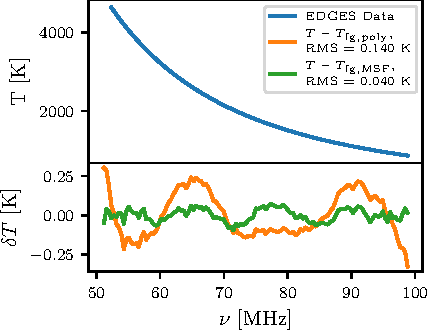
\includegraphics{maxsmooth/figs/Figure1.pdf}
    \caption{An example of the applications of MSFs and \maxsmooth~using the publicly available global 21-cm EDGES low-band experiment data. The top panel shows the EDGES data, blue, and the bottom panel shows the residuals after fitting and removing an unconstrained polynomial, orange, and an MSF, green. The MSF fits the data to a higher degree of accuracy and reveals a systematic that has been partially removed by the polynomial as part of the foreground. The polynomial is given by equation~(2) of \protect\cite{Bowman_edges_2018} and is taken to be 5\textsuperscript{th} order. We use the best fitting 11\textsuperscript{th} order MSF from the built-in library in \maxsmooth~to illustrate the quality of fit recovered.}
    \label{fig:fig0}
\end{figure}

The constrained nature of DCFs, namely that specific derivatives do not cross zero in the domain of interest, makes fitting these functions a non-trivial task. While this has been historically performed with penalised optimization routines such as Basinhopping \citep[][]{Basinhopping} and Nelder-Mead \citep[][]{Nelder-Mead} we find that the use of quadratic programming \citep[][]{qp} is considerably more computationally efficient and reliable. Our DCF code, \maxsmooth~is therefore based on quadratic programming and uses the Python based convex optimisation code, \cvxopt~\citep[ConVeX OPTimization,][]{cvxopt}. A discussion of quadratic programming can be found in Appendix A of \cite{Bevins_maxsmooth_2021}. 

The constraints on a DCF are not explicitly linear but are piecewise linear with various combinations of positive and negative signs on the high order derivatives. For low order, $N$, DCFs testing every combination of positive and negative signs is a computationally inexpensive task. However, this becomes increasingly time-consuming with increasing $N$ and \maxsmooth~uses a `cascading routine' in combination with a directional exploration to quickly search the discrete sign spaces.

DCFs can be formed from a variety of different basis functions and \maxsmooth~has a built-in library. The library is not intended to be complete, and the user can implement their own basis functions. For basis functions in which the number of high order derivatives is not finite, \maxsmooth~constrains derivatives up to order $m = N - 2$. MSFs form the basis of the analysis performed in this chapter and we focus on their uses and applications. However, the description of MSFs can be more broadly applied to DCFs.

In \cref{sec:MSFs} we describe MSFs in more detail. In \cref{sec:qp} we discuss the application of quadratic programming to DCF fitting with reference to \cvxopt~and the piecewise linear constraints on the derivatives. \Cref{sec:Eff} discusses the fitting algorithm implemented by \maxsmooth~and compares its efficiency to alternative optimization routines. In \cref{sec:21} we discuss the use of DCFs in 21-cm cosmology. The application of the fitting routine to the EDGES low band data \citep{Bowman_edges_2018} and data from LEDA \citep{Price_LEDA_2018} is illustrated in \cref{sec:EDGES_fits} and \cref{sec:LEDA_fits}. We conclude in \cref{sec:maxsmooth_conclusions}.

The co-authors of \cite{Bevins_maxsmooth_2021}, Will Handley, Anastasia Fialkov, Eloy de Lera Acedo, Lincoln Greenhill and Danny Price, provided comments on the manuscript that this chapter is based on.

\section{Maximally Smooth Functions}
\label{sec:MSFs}

MSFs are functions which feature no inflection points or zero crossings in higher order derivatives \citep[see][]{Sathyanarayana2015, Sathyanarayana_msf_2017}. The coefficients of the basis functions are constrained such that the $m$\textsuperscript{th} order derivative satisfies
\begin{equation}
    \frac{d^my}{dx^m}~\geq0~~\textnormal{or}~~  \frac{d^my}{dx^m}~\leq0,
    \label{eq:gen_cond}
\end{equation}
where $x$ and $y$ define the independent and dependent variables and for MSFs $m~\ge~2$. More generally for DCFs $m$ can be greater or equal to any value or equal to a select set of derivative orders. \maxsmooth~features seven built-in DCFs which we use for fitting. Their functional forms and derivatives are shown in \cref{tab:basis_functions}.

\begin{landscape}
\begin{table*}
    \centering
    \begin{tabular}{ccc}
        \hline
          Name & Function & Derivatives \\
         \hline
         Normalised Polynomial 
         & \parbox{6cm}{\begin{equation}
             y~=~y_0\sum_{k=0}^{N}~a_{k}~\bigg(\frac{x}{x_0}\bigg)^k
             \label{eq:norm_poly}
         \end{equation}}
         & \parbox{8cm}{\begin{equation*}
            \frac{d^my}{dx^m}~=~y_0~\sum_{k=0}^{N-m}~\frac{(m~+~k)!}{k!}~a_{m+k}~\bigg(\frac{x^k}{x_0^{m+k}}\bigg)
        \end{equation*}} \\
         Polynomial 
         & \parbox{6cm}{\begin{equation}
            y~=~\sum_{k=0}^{N}~a_{k}~x^k \label{eq:additional_basis_a}
         \end{equation}}
         & \parbox{8cm}{\begin{equation*}
            \frac{d^my}{dx^m}~=~\sum_{k=0}^{N-m}~\frac{(m~+~k)!}{k!}~a_{m+k}~x^k
         \end{equation*}} \\
         Difference Polynomial 
         & \parbox{6cm}{\begin{equation}
            y~=~\sum_{k=0}^{N}~a_{k} (x~-~x_0)^k
            \label{eq:additional_basis_b}
         \end{equation}}
         & \parbox{8cm}{\begin{equation*}
            \frac{d^my}{dx^m}~=~\sum_{k=0}^{N-m}~\frac{(m~+~k)!}{k!}~a_{m+k}~(x~-~x_0)^k
         \end{equation*}}\\
         Log Polynomial 
         &  \parbox{6cm}{\begin{equation}
            y~=~\sum_{k=0}^{N}~a_{k}~\log_{10}\bigg(\frac{x}{x_0}\bigg)^k 
            \label{eq:log_poly}
         \end{equation}}
         &  \parbox{8cm}{\begin{equation*}
            \frac{d^my}{d\log_{10}(x/x_0)^m}~=~\sum_{k=0}^{N-m}~\frac{(m~+~k)!}{k!}~a_{m+k}~\log_{10}\bigg(\frac{x}{x_0}\bigg)^k
         \end{equation*}} \\
         Log Log Polynomial 
         & \parbox{6cm}{\begin{equation}
            y~=~10^{\sum_{k=0}^{N}~a_{k}~\log_{10}(x)^k}
            \label{eq:loglog_poly}
         \end{equation}}
         & \parbox{8cm}{\begin{equation*}
            \frac{d^m\log_{10}(y)}{d\log_{10}(x)^m}~=~\sum_{k=0}^{N-m}~\frac{(m~+~k)!}{k!}~a_{m+k}~\log_{10}(x)^k
         \end{equation*}} \\
         Legendre & \parbox{6cm}{\begin{equation}
            y~=~\sum_{k=0}^{N}~a_{k} P_k(z)
            \label{eq:legendre}
         \end{equation}}
         &  \parbox{8cm}{\begin{equation*} 
            \frac{d^my}{dz^m} = \sum_{k=0}^{N-m}~\frac{(-1)^m~P^m_k(z)}{(1-z^2)^{\frac{m}{2}}}
            \end{equation*}} \\
         Exponential 
         & \parbox{6cm}{\begin{equation}
            y~=~y_0\sum_{k=0}^{N}~a_{k}~\exp\bigg(-k~\frac{x}{x_0}\bigg)
         \label{eq:exponential}
         \end{equation}}
         & \parbox{8cm}{\begin{equation*}
            \frac{d^my}{dx^m} = y_0~\sum_{k=0}^{N} \bigg(\frac{-k}{x_0}\bigg)^m a_k \exp\bigg(-k~\frac{x}{x_0}\bigg)
         \end{equation*}}\\
    \end{tabular}
    \caption{The DCF models built-in to \maxsmooth~along with expressions for their $m$\textsuperscript{th} order derivatives. For all functions $y_0$ and $x_0$ are pivot points in the data sets. More details on each DCF function can be found in the text.}
    \label{tab:basis_functions}
\end{table*}
\end{landscape}

Generally, the DCF functions can be decomposed in terms of basis functions, $\phi$ and parameters, $a_k$ as
\begin{equation}
    y~=~\sum_{k=0}^{N}~a_{k}~\phi_k(x).
    \label{eq:general_poly}
\end{equation}
For the first DCF shown in \cref{tab:basis_functions}, the Normalised Polynomial model, the basis functions are given by
\begin{equation}
    \phi_k(x)~=~y_0~\bigg(\frac{x}{x_0}\bigg)^k,
\end{equation} 
where $y_0$ and $x_0$ correspond to a pivot point, defaulted to the mid-point, in the data sets. The normalised nature of this polynomial model ensures that the fit parameters, $a_k$, are of order unity. Here $N$ is the order of the DCF and can take on any value. However, for a given model and data set there is a limiting value beyond which a further increase in $N$ does not increase the quality of the fit and this is illustrated in \cref{sec:EDGES_fits} and \cref{fig:EDGES_basis}. The DCF model will have powers from 0 to $N-1$.

Two more basis functions built-in to \maxsmooth~are given by the Polynomial and Difference Polynomial models where the latter is based on the basis function used in \cite{Sathyanarayana_msf_2017}. The built-in set of models is not meant to be complete with the intention for it to be extended in the future.

The fourth basis function built-in to \maxsmooth, Log Polynomial, produces an MSF in $y - \log_{10}(x)$ space. \maxsmooth~is also capable of fitting a DCF in $\log_{10}(y) - \log_{10}(x)$ space given in \cref{tab:basis_functions} as the Log Log Polynomial model. In this instance the function is constrained by derivatives in $\log_{10}(y) - \log_{10}(x)$ space. This can be advantageous in situations where the foregrounds are expected to take on a power law structure.

The penultimate basis function in the \maxsmooth~library of models is built from the orthogonal Legendre Polynomials, $P_k(z)$, where z is a variable of length $y$ over the range [-1, 1]. The $m$\textsuperscript{th} order derivatives of this model are determined by the Associated Legendre Polynomials, $P^m_k(z)$. By definition the Legendre polynomials are a linear combination of the basis functions of the Normalised Polynomial model. This is true also for the Polynomial model and less trivially for the Difference Polynomial model.

Typically the basis functions are designed so that \cref{eq:general_poly} has a finite number of high order derivatives and is consequently polynomial in nature. However, more elaborate models with an infinite number of derivatives are plausible if we consider these functions to be maximally smooth when all derivatives with $ 2\leq m \leq N-2$ are constrained. The final DCF model built-in to \maxsmooth, the Exponential DCF, is an example of this with exponential basis functions. This model fails at high $N$ where the exponential cannot be computationally calculated. However, it is a useful example of a DCF with infinite derivatives and performs well with low values of $N$. The exact value of $N$ at which this basis begins to fail is determined by the magnitude of the $x$ data. An alternative example of a basis with infinite derivatives that \maxsmooth~is capable of fitting would be a polynomial function with non-integer powers.

Generally, the form of the basis function is important in determining the quality of the residuals and careful exploration of the basis functions are needed in order to draw sensible conclusions about the data set. Again, this is illustrated with an example in \cref{sec:EDGES_fits}. We also note that DCFs fitted in $y - \log_{10}(x)$ space, $\log_{10}(y) - \log_{10}(x)$ space, $y - x$ space or $y - z$ space are not equivalent since the form of the constraints and the function that we minimise are different in each case. This is discussed further in \cref{sec:qp}.

With appropriate normalisation \maxsmooth~will be able to transform any basis function into a `standard' form, which can be solved easily and transformed back into the initial basis function choice. Designing and automating such a normalisation is the subject of ongoing work. Provided this `standard' form is chosen well such that it will always return the best quality fits and is computationally solvable with quadratic programming, the initial choice of basis function will largely be negated. Its form will only be determined by the need of the user to model their foreground using a specific model. For example, in 21-cm cosmology this specific model may be a linearised physical model of the data fitted as an MSF. While normalisation remains absent in \maxsmooth, the user has the ability to input normalised $x$ and $y$ data.

For quadratic programming, the method used here to fit MSFs, it is useful to reformulate \cref{eq:general_poly} as a matrix equation. Explicitly we have discrete data points $y_i$ and $x_i$ which means that $\phi_k(\mathbf{x})$ forms a two dimensional matrix, $\mathbf{\Phi}$. The matrix of basis functions has dimensions $(D\times N)$ where D is the length of $\mathbf{y}$ and $N$, as before, is the order of the function. We write this as
\begin{equation}
    \begin{bmatrix}
    y_0 \\ \vdots \\ y_D
    \end{bmatrix}
    =
    \begin{bmatrix}
    \phi_{00} & \dots & \phi_{0(N-1)} \\
    \vdots & \ddots & \\
    \phi_{D0} & & \phi_{D(N-1)}
    \end{bmatrix}
    \begin{bmatrix}
    a_0 \\ \vdots \\ a_{(N-1)}
    \end{bmatrix},
\end{equation}
where $\phi_{ik} = \phi_k(x_i)$. We can summarise this as
\begin{equation}
    \mathbf{y}~=~\mathbf{\Phi}~\mathbf{a},
    \label{eq:gen_poly_matrix}
\end{equation}
where $\mathbf{a}$ is a column vector of length $N$ representing the parameters. For the polynomial basis function in \cref{eq:additional_basis_a}, the element $\phi_{D0}$, or $\phi_0(x_D)$, has the form $x_D^0$ and $\phi_{0(N-1)}$ has the form $x_0^{(N-1)}$.

Reformulating \cref{eq:gen_cond} in terms of matrices for quadratic programming is more complicated. If we take the definition of the condition with the derivative $\leq 0$ and write this in the form of a matrix for a given derivative order $m$ we find
\begin{equation}
    \begin{bmatrix}
    \frac{d^my}{dx^m}_0 \\
    \vdots \\
    \frac{d^my}{dx^m}_{D} \\
    \end{bmatrix}
    \leq
    \begin{bmatrix}
    0 \\ \vdots \\ 0
    \end{bmatrix},
    \label{eq:derivative_matrices}
\end{equation}
where both matrices are columns of length $D$. Each row in the derivative matrix corresponds to an evaluation of the $m$\textsuperscript{th} order derivative for a given $y_i$ and $x_i$.

We can expand the elements of the derivative matrix out into a matrix of derivative prefactors, $\mathbf{G}$, and the matrix of parameters $\mathbf{a}$, as in \cref{eq:gen_poly_matrix}, which is useful for implementing quadratic programming. This is best illustrated with an example, we will look at the simple case of $N~=~3$ with one constrained derivative $m~=~2$. We will say that our data sets have a length $D~=~4$ and choose the simplest functional form for our MSF given by \cref{eq:additional_basis_a}. In this case $G$ is given by
\begin{equation}
    G_k^m(x_i) = \frac{(m~+~k)!}{k!}~x_i^k,
    \label{eq:prefactors}
\end{equation}
for the range $k = 0$ up to but not including $N-m$. For this problem $k$ has only one value $0$ which would produce a column matrix of elements of length $D$. However, since we need to multiply this by the column matrix $\mathbf{a}$ of length $N$ then the matrix $\mathbf{G}$ should have dimensions of $D \times N$. The additional elements in this instance are $0$ so that the product of these elements with the corresponding elements of $\mathbf{a}$ equals $0$. For example here the evaluation of the second order derivative $\mathbf{Ga}$ for the first data element will be
\begin{equation}
    \frac{d^2y}{dx_0^2} = a_0 0 + a_1 0 + a_2 \frac{(2~+~0)!}{0!}~(x_0)^0.
\end{equation}

Generally, if the row elements of $\mathbf{G}$ have a position from $0 - (N-1)$ then the elements with position $\leq m - 1$ will be $0$. The matrix $\mathbf{G}$ for our specific problem then becomes
\begin{equation}
    \mathbf{G} =
    \begin{bmatrix}
    0 & 0 & G_0^2(x_0) \\
    0 & 0 & G_0^2(x_1) \\
    0 & 0 & G_0^2(x_2) \\
    0 & 0 & G_0^2(x_3) \\
    \end{bmatrix},
\end{equation}
which when multiplied by $\mathbf{a}$ gives us the evaluation of the derivatives as a column matrix with length $D = 4$.

For quadratic programming we need one matrix expression for all of the constraints on our function. Our definition of $\mathbf{G}$ scales with the order of the DCF so that for $N~=~4$ we have
\begin{equation}
    \mathbf{G} =
    \begin{bmatrix}
    0 & 0 & G_0^2(x_0) & G_1^2(x_0)\\
    0 & 0 & G_0^2(x_1) & G_1^2(x_1)\\
    0 & 0 & G_0^2(x_2) & G_1^2(x_2)\\
    0 & 0 & G_0^2(x_3) & G_1^2(x_3)\\
    0 & 0 & 0 & G_0^3(x_0)\\
    0 & 0 & 0 & G_0^3(x_1)\\
    0 & 0 & 0 & G_0^3(x_2)\\
    0 & 0 & 0 & G_0^3(x_3)\\
    \end{bmatrix},
    \label{eq:example_G}
\end{equation}
which includes the prefactors on both the $m = 2$ and $m = 3$ derivatives. We can, therefore, re-write \cref{eq:gen_cond} for $\leq 0$ and \cref{eq:derivative_matrices} as
\begin{equation}
    \mathbf{Ga} \leq \mathbf{0},
    \label{eq:cvx_const}
\end{equation}
where generally $\mathbf{G}$ will have shape $(CD) \times N$ and $\mathbf{0}$ will have a length $CD$. Here $C$ is the total number of constrained derivatives and in the two examples above $C = 1$ and $C = 2$ respectively. We can write the first case in \cref{eq:gen_cond} in one of two ways as $\mathbf{Ga} \geq \mathbf{0}$ or as $-(\mathbf{Ga}) \leq \mathbf{0}$. For the implementation of quadratic programming used in \maxsmooth~the second is the most useful and a full discussion of this can be found in \cref{sec:qp}.

In some cases we find that a DCF with one or more high order derivatives free to cross zero is needed to better fit the data. It is to this effect that the potential to allow zero crossings to the fit is built-in to \maxsmooth. However, \maxsmooth~will not force zero crossings and produce a Partially Smooth Function~(PSF) if it can find a better solution without the need.

\section{Fitting Derivative Constrained Functions Using Quadratic Programming}
\label{sec:qp}

A brief overview of quadratic programming can be found in Appendix A of \cite{Bevins_maxsmooth_2021} and what follows is a discussion of the specific problem of fitting DCFs with quadratic programming.

When fitting a curve using the least-squares method we minimize
\begin{equation}
    \chi^2~=~\sum_k^D~(y_{k}~-~y_{\mathrm{fit,}~k})^2,
\end{equation}
where $y_{\mathrm{fit},~k}$ denotes the elements of the fitted model. We can substitute \cref{eq:gen_poly_matrix} for the fitted model and re-write this in terms of matrices as
\begin{equation}
    \chi^2(\mathbf{a})~=~(\mathbf{y}~-~\mathbf{\Phi}~\mathbf{a})^T~(\mathbf{y}~-~\mathbf{\Phi}~\mathbf{a}),
\end{equation}
where we are looking for solutions of the parameters $\mathbf{a}$ that minimise $\chi^2(\mathbf{a})$. When expanded out this becomes
\begin{equation}
    \chi^2(\mathbf{a}) = \mathbf{y}^T\mathbf{y} - 2 \mathbf{y}^T \mathbf{\Phi} \mathbf{a} + \mathbf{a}^T \mathbf{\Phi}^T~\mathbf{\Phi} \mathbf{a}.
\end{equation}
Since $\mathbf{y}^T\mathbf{y}$ is a constant it is irrelevant for the minimisation problem and we can ignore it. We can also divide through by the factor of $2$ and this leaves
\begin{equation}
    \chi^2(\mathbf{a})~=~\frac{1}{2}~\mathbf{a}^T~\mathbf{Q}~\mathbf{a}~+~\mathbf{q}^T~\mathbf{a},
    \label{eq:chi}
\end{equation}
where
\begin{equation}
    \mathbf{Q}~=~ \mathbf{\Phi}^T~\mathbf{\Phi}~~\textnormal{and}~~ \mathbf{q}^T~=~-\mathbf{y}^T~\mathbf{\Phi}.
\end{equation}

As previously discussed in \cref{sec:MSFs}, the constraint in \cref{eq:gen_cond} is not explicitly linear but is two separately testable linear constraints. The quadratic program solver \cvxopt~minimizes \cref{eq:chi} subject to \cref{eq:cvx_const}. It requires $\mathbf{G}$ and $\mathbf{0}$ as inputs which explains the motivation behind defining the stacked matrix of derivatives as $\mathbf{Ga}$. In \cvxopt~the identity is fixed and we cannot directly constrain the problem via a greater than or equals inequality.

We can initially force all the derivatives to be positive, the first of the two conditions in \cref{eq:gen_cond}, by multiplying each element in $\mathbf{G}$ by a negative sign as discussed in the previous section. However, it will not necessarily be the case that the optimal DCF fit will have an entirely positive or entirely negative set of derivatives. Rather than forcing the entire matrices to produce positive derivatives we can multiply the elements of $\mathbf{Ga}$ corresponding to given derivatives by a negative sign. Consequently, we have to analyse different discrete sets of sign combinations in order to find the best fit. 

We refer to the combination of signs on $\mathbf{G}$ as the \maxsmooth~signs, $\mathbf{s}$, and we can incorporate this into our definition of $\mathbf{G}$ so that it becomes $\mathbf{G}(\mathbf{s})$. $\mathbf{s}$ is a vector of length $C$ and each element is either given by $1$ for a positive sign or $-1$ for a negative sign. For example, in \cref{eq:example_G} since both derivatives are negative the \maxsmooth~signs are $s = [1,~1]$. For an $N$\textsuperscript{th} order MSF there are $N-2$ derivatives with $m~\ge~2$, consequently, there are $2^{(N~-~2)}$ sign combinations. For low order $N$ we can explore this space exhaustively at reasonable computational cost with \cvxopt. However, as $N$ becomes larger, the total number of sign combinations rapidly increases. While $N~=~4$ has $4$ potential sign combinations, we find that $N~=~13$ has $2048$. This would mean performing an exponentially increasing number of \cvxopt~fits, which will become increasingly time-consuming. An alternative approach, navigating through the discrete sign spaces, is detailed in \cref{sec:Eff}.

We can visualise \cref{eq:gen_cond} by varying the parameters of an optimal MSF fit over a given range to get a better understanding of the constraints. In order to perform this analysis, we use a simulated noiseless global 21-cm foreground following $x^{-2.5}$. We perform a 5\textsuperscript{th} order MSF fit with \maxsmooth~on this data using \cref{eq:additional_basis_a} to find the optimal foreground parameters. While this fit will not return the best $\chi^2$, as shown in \cref{fig:poly_params}, it is sufficient to allow us to investigate how variation in the parameters affects the constraints. We vary each parameter's value $200\%$ either side of the optimum found and sample these ranges using 100 points.

\cref{fig:poly_params}, left panel, shows the parameter space for the fit described above. Black regions in the figure are combinations of parameters for which the condition in \cref{eq:gen_cond} is violated. The coloured regions are regions in which the condition is upheld where their colour is related to the \maxsmooth~sign combinations. Each panel in the figure shows the parameter space for two of the five parameters, and the contour lines show the values of $\chi^2$ across the parameter ranges. While varying the parameters relevant to each panel, we maintain all others at their optimal values found with \maxsmooth. The contour lines help us to determine correlations between the parameters, and this is particularly useful when fitting a physically motivated DCF.

\begin{figure*}
    \centering
    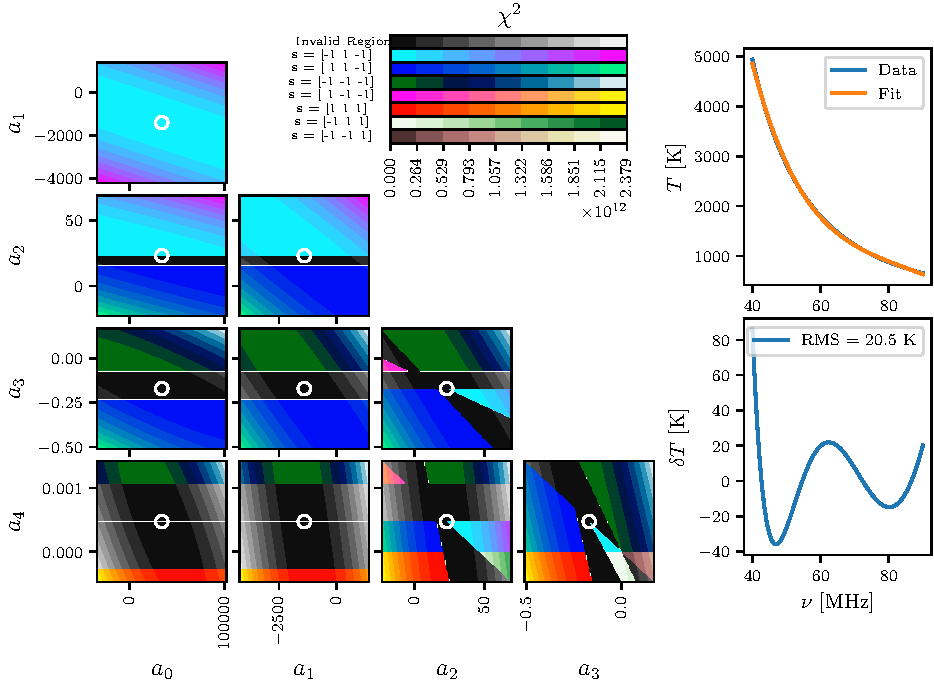
\includegraphics{maxsmooth/figs/Figure2.pdf}
    \caption{\textbf{Left:} The parameter space of a 5\textsuperscript{th} order MSF of the form given by \cref{eq:additional_basis_a}, fit to data generated with $y = x^{-2.5}$. The tested parameter ranges are taken to be $200\%$ on either side of the optimal results found by \maxsmooth. We maintain the optimal parameter values for three of the parameters when varying the two corresponding to each panel. Black regions of the graph show parameter combinations that violate \cref{eq:gen_cond} and coloured regions correspond to viable regions. The central sampled point, highlighted by the white circles~(at their centres), in each panel corresponds to the optimum parameters and the optimum \maxsmooth~sign combination on the derivatives. Transitions through regions of violation correspond to changes in the sign of one or more high order derivatives. A change in sign of parameter $a_4$ corresponds to a change in the sign of the final constrained derivative. Since this derivative is a constant, there is no violated region between these two possible sign combinations. \textbf{Top Right:} The data and the fitted MSF, where $T$ represents the measured sky temperature and $\nu$ is the frequency. \textbf{Bottom Right:} The residuals after subtracting the fitted MSF from the data.}
    \label{fig:poly_params}
\end{figure*}

Transitions through a region of violation between viable regions correspond to changes in the \maxsmooth~sign of one or more of the derivatives. This is illustrated by the use of different colour maps across the different viable regions. For example, in the panel corresponding to variation in $a_0$ and $a_2$ for $a_2 \leq 15$ $s = 1$ and for $a_2 \geq 25$ $s = -1$ for the $m = 2$ derivative. The transitions become more complex when varying parameters $a_2$, $a_3$ and $a_4$ because these parameters affect the magnitude and signs of multiple high order derivatives. We also see transitions between regions of different sign combinations when $a_4$ switches sign. %This causes the final constrained derivative to switch sign because it is a constant multiplied by $a_4$. 
There is no region of violation between these viable regions because a constant value of $a_4 = 2.5\times 10^{-4}$ meets the MSF constraint, as will a constant value of $0$ or $a_4 = -2.5\times 10^{-4}$.

The equivalent graph in 5 dimensions, varying all parameters around their optimal values, would feature 5 dimensional convex faceted regions in which \cref{eq:gen_cond} is met with a unique set of \maxsmooth~signs. This concept scales up and down to higher and lower dimensions of parameter space.

The parameters $a_0$ and $a_1$ do not affect the constrained derivatives of the MSF or the validity of the conditions, and the associated colour map gives the optimum \maxsmooth~signs. Since the central sample point of each panel corresponds to the optimum parameters for the fit, this will always be a viable region and will have the same \maxsmooth~sign combination as the panel corresponding to $a_0$ and $a_1$. \cref{fig:poly_params} illustrates this point and, where visible, the central viable sample point always corresponds to derivatives of order $m = 2,~3$ and $4$ having $\mathbf{s} = [-1,~1,~-1]$. 

Where the central sample point in each panel is not visible, this is a relic of the sample rate across the parameter space. For example in the panel corresponding to variation of $a_0$ and $a_4$, between the two large regions of violation there is a single value of $a_4$, the optimum, that meets the condition given by \cref{eq:gen_cond}. The tight constraints around the optimum values in the four panels in the bottom left corner of the figure are due to the independence of the constraints for an MSF on $a_0$ and $a_1$ and the strong dependence on $a_3$ and $a_4$.

We performed the equivalent fit with the logarithmic basis that has derivatives constrained in $\log_{10}(y) - \log_{10}(x)$ space. The associated parameter graph can be found in Appendix B in \cite{Bevins_maxsmooth_2021}, and a comparison with the graph presented in this section shows that the constraints are much less severe in logarithmic space. The weak constraints mean that all the discrete sign combinations on the derivatives have similar minimum $\chi^2$ values. This becomes a problem when attempting to quickly search the discrete \maxsmooth~sign spaces and is discussed further in \cref{sec:badproblems}.

Generally, the above conclusion will be specific to the data being fitted here, and this analysis is not a complete exploration of the basis functions available. However, since the basis functions in $y - x$ space are all related by linear combinations of each other, we find similar parameter distributions for all. Importantly, the analysis highlights the effect that the choice of basis function has on the quality of fit and ease of fitting, as well as demonstrating the constrained nature of MSFs. These plots can be produced using \maxsmooth~for any DCF fitting problem.

\section{Navigating Discrete Sign Spaces}
\label{sec:Eff}

This section discusses in more detail the fitting problem, defines the \maxsmooth~algorithm and compares its efficiency with an alternative fitting algorithm. To restate concisely the problem being fitted we have
\begin{equation}
    \begin{split}
        &\min_{a,~s}~~\frac{1}{2}~\mathbf{a}^T~\mathbf{Q}~\mathbf{a}~+~\mathbf{q}^T~\mathbf{a}, \\
        &\mathrm{s.t.}~~\mathbf{G(s)~a} \leq \mathbf{0}.
    \end{split}
\end{equation} 
A `problem' in this context is the combination of the data, order, basis function and constraints on the DCF. 

With \maxsmooth~we can test all possible sign combinations. This is a reliable method and, provided the problem can be solved with quadratic programming, will always give the correct global minimum. When the problem we are interested in is `well-defined', we can develop a quicker algorithm that searches or navigates through the discrete \maxsmooth~sign spaces to find the global minimum. Each sign space is a discrete parameter space with its own global minimum, as discussed in \cref{sec:qp}. Using quadratic programming on a fit with a specific sign combination will find this global minimum, and we are interested in finding the minimum of these global minima.

A `well-defined' problem is one in which the discrete sign spaces have large variance in their minimum $\chi^2$ values and the sign space for the global minimum is easily identifiable. In contrast, we can have an `ill-defined' problem in which the variance in minimum $\chi^2$ across all sign combinations is small. This concept of `well-defined' and `ill-defined' problems is explored further in the following two subsections.

\subsection{Well-defined Problems and Discrete Sign Space Searches}
\label{sec:well_defined}

\subsubsection{The $\chi^2$ Distribution}

We investigate the distribution of $\chi^2$ values, shown in \cref{fig:ChiDistSim21}, for a 10\textsuperscript{th} order MSF fit of the form given by \cref{eq:log_poly} to a simulated 21-cm foreground, like that shown in \cref{fig:poly_params}. We add Gaussian noise with a standard deviation of $0.5$ to the foreground. For a typical 21-cm experiment this noise is unrealistic and would mask any potential signal in the data, however, it illustrates the behaviour of the \maxsmooth~algorithm when fitting a difficult problem.

In \cref{fig:ChiDistSim21}, a combination of all positive derivatives~(negative signs) and all negative derivatives~(positive signs) corresponds to sign combination numbers 255 and 0 respectively. Specifically, the \maxsmooth~signs, $\mathbf{s}$, are related to the sign combination number by its $C$ bit binary representation, here $C = (N -2)$. In binary, the sign combination numbers run from $00000000$ to $11111111$. Each bit represents the sign on the $m$\textsuperscript{th} order derivative, with a $1$ representing a negative \maxsmooth~sign. For example, the sign combinations surrounding number 25 are shown in \cref{tab:binary}.

\begin{table}
    \centering
    \begin{tabular}{ccc}
        \hline
         Sign & Binary & \maxsmooth  \\
         Combination &  & Signs, $\mathbf{s}$  \\
         \hline
         23 & 00010111 & [+1, +1, +1, -1, +1, -1, -1, -1]\\
         24 & 00011000 & [+1, +1, +1, -1, -1, +1, +1, +1]\\
         25 & 00011001 & [+1, +1, +1, -1, -1, +1, +1, -1]\\
         26 & 00011010 & [+1, +1, +1, -1, -1, +1, -1, +1]\\
         27 & 00011011 & [+1, +1, +1, -1, -1, +1, -1, -1]\\
    \end{tabular}
    \caption{The table illustrates the relationship between the binary representation of the sign combination number and the \maxsmooth~signs, $\mathbf{s}$. A $1$ in the $(N - 2)$ bit binary representation for an MSF corresponds to a negative \maxsmooth~sign~(positive derivative). The signs and their respective combination numbers are used in the fitting routine and for the visualisation of the $\chi^2$ distribution, as shown in \cref{fig:ChiDistSim21}.}
    \label{tab:binary}
\end{table}

Although we note that \cref{fig:poly_params} corresponds to a different problem, we would expect a similar parameter space for the fit performed here. Each region in the equivalent figure would correspond to a single sign combination, and the associated minimum $\chi^2$ value in the regions would give us the data that informs \cref{fig:ChiDistSim21}.

\begin{figure}
    \centering
    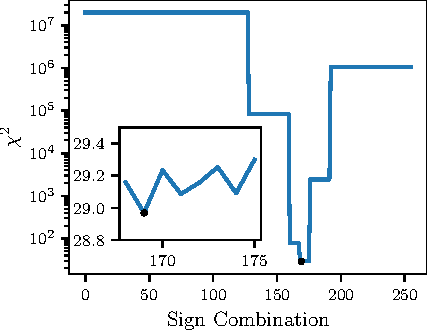
\includegraphics{maxsmooth/figs/Figure3.pdf}
    \caption{The $\chi^2$ values for the discrete sign combinations on the derivatives for a 10\textsuperscript{th} order MSF fit in $y - \log(x)$ space to a simulated 21-cm foreground. Sign combination 0 corresponds to negative derivatives~(positive \maxsmooth~signs) and 255 corresponds to positive derivatives~(negative \maxsmooth~signs). The signs and sign combination numbers are related by the $(N-2)$ bit binary representation of the number. The global minimum is shown as a single black data point. In the insert, the distribution around the global minimum is shown, and here the axis have the same meaning as in the main plot.}
    \label{fig:ChiDistSim21}
\end{figure}

The distribution appears to be composed of smooth steps or shelves; however, when each shelf if studied closer, we find a series of peaks and troughs. This can be seen in the subplot of \cref{fig:ChiDistSim21} which shows the distribution in the neighbourhood of the global minimum found in the large or `global' well. This type of distribution with a large variance in $\chi^2$ is characteristic of a `well-defined' problem. We use this example $\chi^2$ distribution to motivate the \maxsmooth~algorithm outlined in the following subsection.

\subsubsection{The \maxsmooth~Sign Navigating Algorithm}

Exploration of the discrete sign spaces for high $N$ can be achieved by exploring the spaces around an iteratively updated optimum sign combination. The \maxsmooth~algorithm begins with a randomly generated set of signs for which the objective function is evaluated, and the optimum parameters are found. We flip each individual sign one at a time, beginning with the lowest order constrained derivative first. When the objective function is evaluated to be lower than that for the current optimum sign combination, we replace it with the new set and repeat the process in a `cascading' routine until the objective function stops decreasing in value.

The local minima shown in \cref{fig:ChiDistSim21} mean that the cascading algorithm is not sufficient to consistently find the global minimum. We can demonstrate this by performing 100 separate runs of the cascading algorithm on the simulated 21-cm foreground. We use \cref{eq:log_poly} with $N = 10$ to model the MSF as before. We find the true global minimum 79 times and a second local minimum 21 times. For an MSF fit to this simulated data the difference in these local minima is insignificant, $\Delta \chi^2 = 0.12$. However, we see the same behaviour with real data sets from EDGES and LEDA, and when performing joint fits of foregrounds and signals of interest $\Delta \chi^2$ can greatly increase.

The abundance of local minima is determined by the magnitude and presence of signals, systematics and noise in the data. When jointly fitting a signal/systematic model with a DCF foreground, the signal/systematic parameters are estimated by another fitting routine in which \maxsmooth~is wrapped. The initial parameter guess will not be a perfect representation of any real systematic or signal. This, along with a large noise, can produce a large difference between the true foreground and the `foreground' being modelled, causing the presence of local minima to become more severe.

To prevent the routine terminating in a local minimum, we perform a complete search of the sign spaces surrounding the minimum found after the cascading routine. We refer to this search as a directional exploration and impose limits on its extent. In each direction, we limit the number of sign combinations to explore, and we limit the maximum allowed increase in $\chi^2$ value. We prevent repeated calculations of the minimum for given signs and treat the minimum of all tested signs as the global minimum.

\begin{figure}
    \centering
    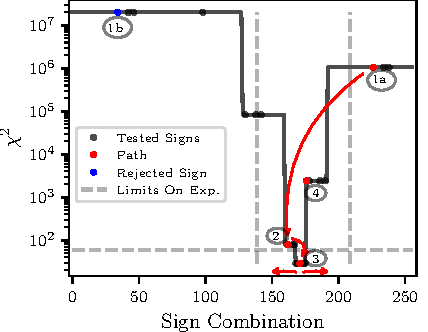
\includegraphics{maxsmooth/figs/Figure4.pdf}
    \caption{The cascading and directional exploration algorithm in practice against the entire $\chi^2$ distribution for the fit to the simulated 21-cm experiment data. The red arrows show the approximate path of the cascade and directional exploration. The limits on the directional exploration are also shown as dashed grey lines. The point~(1a) shows the initial random starting point and point~(1b) shows a rejected sign combination in the cascade routine from~(1a) to~(2). Point~(2) is an accepted step through the cascade with a $\chi^2$ value smaller than the previous minimum. Point~(3) marks the end of the cascade and the start of the left directional exploration. Finally, point~(4) illustrates the end of the right directional exploration when the $\chi^2$ value exceeds the limit on the directional exploration. The black dots mark the entirety of the searched sign combinations.}
    \label{fig:Run_snapshots}
\end{figure}

We run the consistency test again, with the full \maxsmooth~algorithm, and find that for all 100 trial fits we find the same $\chi^2$ found when testing all sign combinations. In \cref{fig:Run_snapshots} the red arrows show the approximate path taken through the discrete sign spaces against the complete distribution of $\chi^2$. Point~(1a) shows the random starting point in the algorithm, and point ~(1b) shows a rejected sign combination evaluated during the cascade from point~(1a) to~(2). Point~(2), therefore, corresponds to a step through the cascade. Point~(3) marks the end of the cascade and the start of the left directional exploration. Finally, point~(4) shows the end of the right directional exploration where the calculated $\chi^2$ value exceeds the limit on the directional exploration.

The global well tends to be associated with signs that are all positive, all negative or alternating. We see this in \cref{fig:ChiDistSim21} where the minimum falls at sign combination number 169 and number 170, characteristic of the derivatives for the simulated 21-cm foreground, corresponds to alternating positive and negative derivatives from order $m = 2$. Standard patterns of derivative signs can be seen for all data following approximate power laws. All positive derivatives, all negative and alternating signs correspond to data following the approximate power laws $y\approx x^{k}$, $y\approx -x^{k}$, $y\approx x^{-k}$ and $y\approx -x^{-k}$~(see Appendix C in \cite{Bevins_maxsmooth_2021}). 

The \maxsmooth~algorithm assumes that the global well is present in the $\chi^2$ distribution, and this is often the case. The use of DCFs is primarily driven by a desire to constrain previously proposed polynomial models to foregrounds. As a result, we would expect that the data being fitted could be described by one of the four approximate power laws highlighted above and that the global minimum will fall around an associated sign combination. In rare cases the global well is not clearly defined and this is described in the following subsection.

\subsection{Ill-defined Problems and their Identification}
\label{sec:badproblems}

We can illustrate an `ill-defined' problem, with a small variation in $\chi^2$ across the \maxsmooth~sign spaces, by adding a 21-cm signal into the foreground model and fitting this with a 10\textsuperscript{th} order logarithmic MSF defined by \cref{eq:loglog_poly}. We take an example signal model from \cite{Cohen_global_2017} and add Gaussian noise with a standard deviation of $20$~mK more typical of a 21-cm experiment. The resultant $\chi^2$ distribution with its global minimum is shown in the top panel of \cref{fig:bad_problem_chi}.

The global minimum, shown as a black data point, cannot be found using the \maxsmooth~algorithm. The cascading algorithm may terminate in any of the approximately equal minima, and the directional exploration will then quickly terminate because of the limits imposed.

\begin{figure}
    \centering
    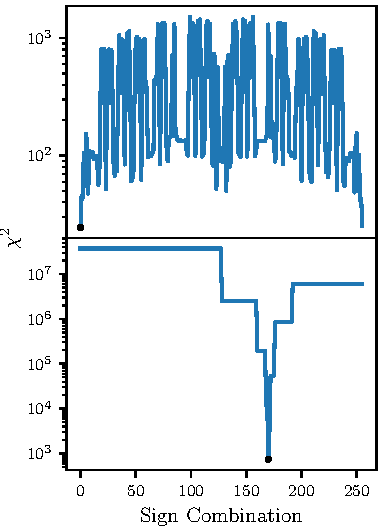
\includegraphics{maxsmooth/figs/Figure5.pdf}
    \caption{\textbf{Top Panel:} The $\chi^2$ distribution found when fitting simulated 21-cm experiment data with the logarithmic basis function, \cref{eq:loglog_poly}. The distribution has a noise like structure and is difficult to solve with the \maxsmooth~sign navigating algorithm. However, the global minimum can be found by testing all sign combinations with \maxsmooth. The symmetric nature of the distribution stems from the symmetric nature about 0 of the high order derivatives in logarithmic space. \textbf{Bottom Panel:} The same as above using a normalised polynomial given by \cref{eq:norm_poly}. The distribution is clearly defined and easily searchable with the sign navigating routine. The difference between this result and that shown above can be used to understand what makes a problem `ill-defined'.}
    \label{fig:bad_problem_chi}
\end{figure}

If we repeat the above fit and perform it with \cref{eq:norm_poly} we find that the problem is well-defined with a larger $\chi^2$ variation across sign combinations. This is shown in the bottom panel of \cref{fig:bad_problem_chi}. The results, when using \cref{eq:loglog_poly}, are significantly better than when using, \cref{eq:norm_poly} meaning it is important to be able to solve `ill-defined' problems. This can be done by testing all \maxsmooth~signs, but knowing when this is necessary is important if you are expecting to run multiple DCF fits to the same data set. We can focus on diagnosing whether a DCF fit to the data is `ill-defined' because a joint fit to the same data set of a DCF and signal of interest will also feature an `ill-defined' $\chi^2$ distribution.

We can identify an `ill-defined' problem by producing the equivalent of \cref{fig:bad_problem_chi} using \maxsmooth~and visually assessing the $\chi^2$ distribution for a DCF fit. Alternatively, we can use the parameter space plots to identify whether the constraints are weak or not, and if a local minimum is returned from the sign navigating routine then the global minimum in these plots will appear off-centre.

\begin{figure}
    \centering
    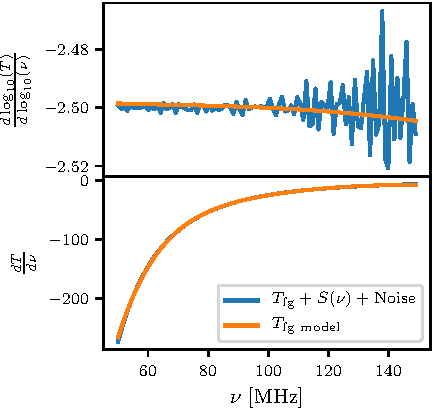
\includegraphics{maxsmooth/figs/Figure6.pdf}
    \caption{The approximated first derivatives, blue lines, of the mock 21-cm experiment data in logarithmic, top panel, and linear, bottom panel, spaces which correspond to DCF fits performed using \cref{eq:loglog_poly} and \cref{eq:norm_poly} respectively. Also shown as orange lines are the approximate first derivatives of the respective best fits for comparison. The large variance of the first derivative of the data in logarithmic space highlights that there are many different ways to fit this data set `well' producing the $\chi^2$ distribution we see in \cref{fig:bad_problem_chi}.}
    \label{fig:bad_prob_derivatives}
\end{figure}

Assessment of the first derivative of the data can also help to identify an `ill-defined' problem. For the example problem this is shown in \cref{fig:bad_prob_derivatives} where the derivatives have been approximated using $\Delta y/ \Delta x$. Higher order derivatives of the data will have similarly complex or simplistic structures in the respective spaces. There are many combinations of parameters that will provide smooth fits with similar $\chi^2$ values in logarithmic space, leading to the presence of local minima. This issue will also be present in any data set where the noise or signal of interest are of a similar magnitude to the foreground in $y - x$ space.

\subsection{Comparison With Basinhopping and Nelder-Mead Methods}
\label{sec:basinhopping}

For comparison of the two methods, testing all sign combinations and navigating through sign spaces, we generate a signal $y$ with polynomial dependence on the coordinate $x$ and a Gaussian random noise with a standard deviation of $0.5$
\begin{equation}
    y~=~0.6~+~2~x~+~4x^3~+~9x^4~+~\textnormal{noise}.
    \label{eq:poly_data}
\end{equation}
We fit this data with a 10\textsuperscript{th} order MSF of the form described by \cref{eq:norm_poly} and assess the $\chi^2$ distribution to find that the problem is well-defined. This is as expected since the data follows an approximate $x^k$ power law, and we are fitting in linear space.

\begin{figure}
    \centering
    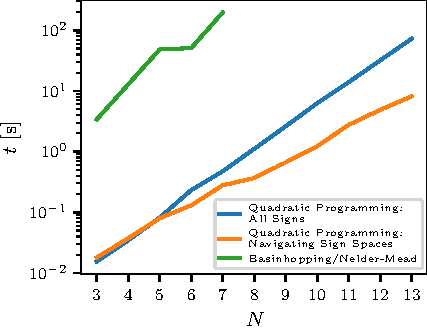
\includegraphics{maxsmooth/figs/Figure7.pdf}
    \caption{ The time taken by \maxsmooth~to fit MSFs of varying order N to the data, described by \cref{eq:poly_data} using the two built-in quadratic programming methods. For comparison, the time taken by a Basinhopping/Nelder-Mead routine is also shown up to $N = 7$ after which the routine fails to find the optimum solutions without adjustments to the routine parameters. All the fits were performed with \cref{eq:norm_poly} and on the same computing hardware.}
    \label{fig:times}
\end{figure}

The algorithm run time becomes a significant issue when performing joint fits of foregrounds, signals of interest and/or systematics in which multiple DCF fits have to be performed. The time taken to perform both in-built \maxsmooth~routines is shown in \cref{fig:times}. It is quicker to partially sample the available spaces for high $N$ than testing all sign combinations, and as discussed for `well-defined' problems this will return the minimum $\chi^2$. 

The runtime of the sign navigating routine is dependent on the starting sign combination, the limits imposed on the directional exploration (which is the dominating factor) and the width of the global well. There is no consistent measure of the difference in time taken to fit the data between the two \maxsmooth~methods. However, for the sign navigating routine we are inevitably fitting for a smaller number of the sign combinations than when testing all.

\cref{fig:times} also shows the time taken to fit the data with \cref{eq:norm_poly} using a Basinhopping routine followed by a Nelder-Mead algorithm, hereafter referred to as BHNM. These two algorithms have been previously used either separately or in conjunction for fitting MSFs \citep{Sathyanarayana2015, Sathyanarayana_msf_2017, Singh_edges_2019}. We find that the BHNM method is approximately two orders of magnitude slower than \maxsmooth. Between $N = 3$ and $7$ we find a maximum percentage difference in $\chi^2$ of $\approx 0.04\%$ when comparing the BHNM method with the results from \maxsmooth.

The primary difference in the approaches comes from the division of the parameter space into discrete sign spaces. The BHNM method attempts to search the entire parameter space and penalises parameter combinations that violate \cref{eq:gen_cond}. However, assessment of \cref{fig:poly_params} highlights that this is not a convenient method because across the whole parameter space there are multiple local minima with different sign combinations and transitioning from one `basin' to another is not trivial for a heavily constrained parameter space. By dividing the space up into discrete sign spaces with \maxsmooth, we can test the entirety of the parameter space, unlike when using the BHNM method, guaranteeing we find the global minimum. We could perform the same division of the space and in each discrete sign space perform a Nelder-Mead or equivalent routine, however we use quadratic programming because it is designed specifically for fast and robust constrained optimisation.

For the BHNM method, we show here only fits up to $N=7$ after which it begins to fail without further adjustment of the routine parameters. The freedom to adjust these parameters can be considered a disadvantage that leaves the user to determine whether the routine parameters they have chosen produce a true global minimum. In contrast, \maxsmooth~is designed to reliably give the optimum result, with the only adjustable routine parameters being the total number of \cvxopt~iterations and the directional exploration limits.

All the fits performed in this section were done using the same computing hardware.

\section{Applications for 21-cm Cosmology}
\label{sec:21}

\subsection{The Recovery of Model 21-cm Signals}

A discussion of MSFs and a comparison to unconstrained polynomials for global 21-cm cosmology can be found in \cite{Sathyanarayana_msf_2017}. Foreground modelling with high order MSFs is shown to accurately recover global 21-cm signals in simulated data and unconstrained polynomials are shown to introduce additional turning points, when compared to those in a mock signal. The number of additional turning points is shown to increase with polynomial order. The addition of extra turning points can obscure the signal of interest and lead to the false identification of systematics. In the following subsections, we look at fitting foregrounds for 21-cm experiments with DCFs and compare these to unconstrained polynomial fits. 

Deviations from a smooth structure can be introduced in data by experimental systematics, or they can be intrinsic to the foreground. In the case of a smooth foreground, by using PSFs we can correct for non-smooth structure directly with our foreground model rather than separately fitting systematics. PSFs allow for zero crossings in the high order derivatives, but remain more constrained than traditionally used polynomial fits. However, lifting constrains on a DCF model has the potential to also result in signal loss, where the level of signal loss is dependent on the presence of non-smooth structure in the foreground and the number of lifted constraints.

In the following analysis, the quality of the fit in terms of Root Mean Square~(RMS) is of secondary importance. An unconstrained high order polynomial will generally produce residuals with a lower RMS than a DCF. However, a correctly constrained DCF will leave behind the structure of a signal in the residuals, meaning it can be identified easily. As a measure of signal structure in the residuals, we take the number of turning points, $p$ as used by \cite{Sathyanarayana_msf_2017}. The global 21-cm signal is expected to have a distinct number of turning points, $2 - 3$, across the bandwidth $~40 - 200$~MHz determined by various astrophysical processes~(see \cref{ch:introduction}). The successful application of DCFs in identifying global signals, being reliant on the presence of non-smooth structure in the data, is therefore bandwidth dependent. However, a comparison of the number of turning points in a mock signal to the residuals after removing a DCF fit from simulated data including the same mock signal will help to identify the degree to which DCFs preserve signals.

\subsubsection{DCFs and 21-cm cosmology}

\begin{figure*}
    \centering
    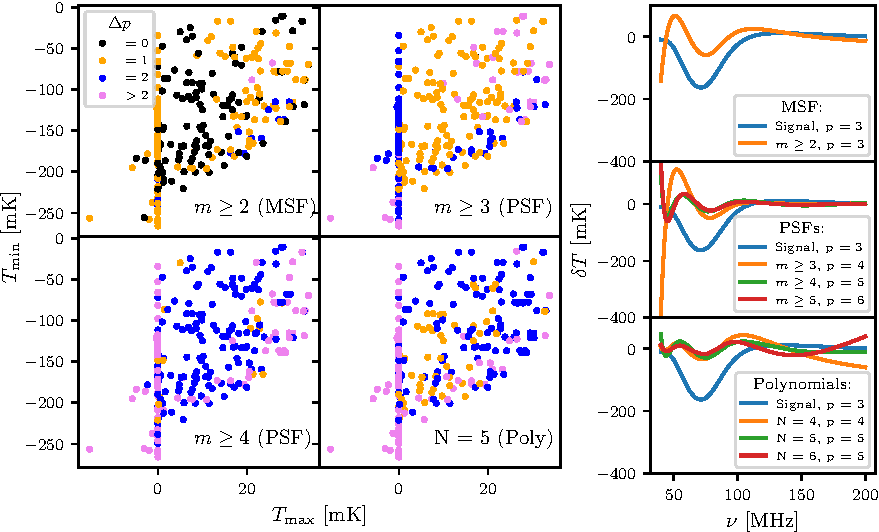
\includegraphics{maxsmooth/figs/Figure8.pdf}
    \caption{\textbf{Left:} The difference in the number of turning points between the fit residuals and the simulated signal, $\Delta p = p_\mathrm{Fit~Residuals} - p_\mathrm{Signal}$, as a function of the maximum and minimum temperatures of the signal for a smooth foreground model. This is shown for four different foreground models, and in each panel the data points correspond to one of the $264$ mock data sets considered. The graph shows that the MSF fit is the most likely model to return the structure of the signal, and that a correctly constrained PSF can more frequently preserve the signal than an unconstrained low order polynomial. It also shows that the fit quality is dependent on the maximum and minimum temperatures of the signal. All the DCF fits used to produce this graph were logarithmic and 13\textsuperscript{th} order. \textbf{Right:} Shown are examples of how the addition of allowed zero crossings in the high order derivatives of a DCF can affect the residuals and how accurately they preserve the turning points of any signal present. We use a signal model, blue line in all panels, from the theoretically motivated set presented in \protect\cite{Cohen_global_2017} along with a model of a 21-cm experiment foreground. Fits with an MSF and polynomials are also shown for comparison with the number of turning points, $p$, displayed for each of the residuals~(see legend for details). While the residuals after fitting and removing an MSF do not identically match the signal, it is the best representation of the tested foreground models. In this case, the residuals represents a smooth baseline subtracted version of the signal as discussed in \citep{Sathyanarayana_msf_2017}.}
    \label{fig:PSF_comp}
\end{figure*}

To compare the performance of DCFs and unconstrained polynomials, we use the sample of 264 signal models, $S(\nu)$ over the bandwidth $\nu = 40 - 200$~MHz, presented in \cite{Cohen_global_2017} and used by \cite{Singh_saras2_2018}. The models are provided by A. Fialkov and are publicly available at: \url{https://people.ast.cam.ac.uk/~afialkov/Collab.html}. We add to these models a foreground given by a $\nu^{-2.5}$ power law to produce simplistic mock data sets. The data sets are noiseless and while this is unrealistic, we would not expect the addition of noise to obscure any larger signal structure present in the data from a 21-cm experiment with a low radiometer noise. We fit each simulated data set with an MSF, low order unconstrained polynomials and a set of PSFs. All the fitted DCF foreground models are 13\textsuperscript{th} order and of the form given by \cref{eq:loglog_poly}. We test all sign combinations for the DCF fits in this section for reasons that were explained in \cref{sec:badproblems} and find that the chosen DCF model and order provides the best fits after testing the built-in \maxsmooth~models.

\cref{fig:PSF_comp}, left panel, shows the difference in the number of turning points, $\Delta p$ for the residuals, $p_\mathrm{Fit~Residuals}$, and for the signal, $p_\mathrm{Signal}$, using four different foreground models as a function of the maximum brightness temperature, $T_\mathrm{max}$, and minimum temperature, $T_\mathrm{min}$, of the simulated signal. Each data point corresponds to one of the $264$ mock data sets and $\Delta p = 0$ signifies that the residuals have the same number of turning points as the signal. The unconstrained polynomial fits have the same functional form as the DCFs.

We can quantify the probability of returning residuals with the same number of turning points as the model signals. \cref{tab:table1} shows the total number of residuals for each fit type that returned the same $p$ as the simulated signals and 1 or 2 additional turning points. The MSF fits return $p_\mathrm{Signal}$ for $44\%$ of the mock data sets and $99\%$ of the time it returns at most $p_\mathrm{Signal}$ plus 2 additional turning points. They are the most likely, of the tested foreground models to return the correct number of turning points. The equivalent figures for the 5\textsuperscript{th} order logarithmic unconstrained polynomial, one of the most frequently used foreground fits in 21-cm cosmology, are $0\%$ and $64\%$ and for the PSF with $m \geq 3$ they are $0.004\%$ and $85\%$. The statistics suggest that modelling foregrounds with MSFs and well constrained PSFs can frequently result in residuals that closely follow the structure of the signal. We include in the statistics the cases with 1 or 2 additional turning points because the signals should still be identifiable in the residuals. A joint fit of a foreground model plus a signal model in these instances should return an approximately correct parameterisation of the signal model.

\begin{table}
    \centering
    \begin{tabular}{ccccc}
        \hline
          & $m\geq2$ & $m\geq3$ & $m\geq4$ &$N = 5$ \\
          & (MSF) & (PSF) & (PSF) & (Poly) \\
         \hline
         $p_{\mathrm{~Signal}}$ & 116 & 1 & 0 & 0 \\
         $p_{\mathrm{~Signal}}+1$ & 132 & 135 & 15 & 52 \\
         $p_{\mathrm{~Signal}}+2$ & 14 & 88 & 147 & 116 \\
    \end{tabular}
    \caption{The table shows the total number of fits, using one of four foreground models, to the smooth foreground plus signal simulations from \protect\cite{Cohen_global_2017} that have residuals with the same number of turning points as the signal, $p_\mathrm{~Signal}$. The data corresponds to that shown in the left panel of \cref{fig:PSF_comp}. We also show instances where the recovered residuals have one or two additional turning points.}
    \label{tab:table1}
\end{table}

\subsubsection{Example Residuals}

Also shown in \cref{fig:PSF_comp}, right panel, is an example of the fits for a given model and this is akin to Fig.7 in \cite{Sathyanarayana_msf_2017}. We see that an MSF, top panel, while not identically recovering the signal but rather a smooth baseline subtracted version does preserve the three turning points of the model signal as expected. The example residuals from the unconstrained polynomial fits shown in the bottom right panel of \cref{fig:PSF_comp} show a larger disparity with the structure of the model 21-cm signal than the MSF fit. The PSF with derivatives of order $m \geq 3$ constrained,  middle panel, produces residuals with one additional turning point. The behaviour at low frequency of the DCF fits is consistent across all the 264 tested models. It is a by-product of the basis choice, the frequency of data sampling and the steep nature of the foreground at low frequencies. We can alleviate some of these issues by increasing the sampling rate of our mock experiment and by reducing the bandwidth. However, the dominant cause is the basis function choice.

In logarithmic space, any non-smooth variations in the data and derivatives are amplified, as shown in \cref{sec:badproblems}. Since the mock data set here is noiseless, the only non-smooth structure comes from the signal. However, the data is predominately smooth at high frequency and so the optimum fit tends to be an accurate representation of the foreground in this region and poorer at lower frequencies. The additional turning points when comparing the MSF and PSFs are also seen at low frequencies for the same reason. Despite the above, we maintain the full bandwidth, the same sampling rate and the logarithmic basis function in this analysis. We do this because this basis function gives us the best fitting DCF models, and in a real experiment our knowledge of any present signal of interest will be too poor to constrain the bandwidth.

We have not analysed the full family of possible PSFs or unconstrained polynomials. Removing constraints on the lower order derivatives first will have the largest effect on the structure of the residuals, and consequently we have extensively analysed the effects of lifting the restrictions on the 2\textsuperscript{nd} and 3\textsuperscript{rd} order derivatives. We have, however, found evidence to suggest that MSFs and well constrained PSFs can recover signal structure to a higher degree of accuracy than unconstrained polynomials in the case of a smooth foreground. If the foreground features additional non-smooth structure, we may expect that an appropriately constrained PSF will act as an MSF. Determination of the appropriate constraints on a PSF will depend on the structure of the data, the expected structure of the signal in the data and the quality of the fit in terms of $\chi^2$.

\subsubsection{Identifiable 21-cm Signals and Limitations of DCFs}

The left panel of \cref{fig:PSF_comp} is useful for 21-cm cosmology, in characterising the signals most likely to be detectable using DCFs. We find that MSFs and $m \geq 3$ PSFs will best recover signals with approximately $T_\mathrm{min} \geq -225$~mK and $T_\mathrm{max} \geq 0$~mK. We would expect this to be true generally because these signal models have complex structures and feature the strongest deviations from the smooth foreground. For the coldest models with $T_\mathrm{min} \leq -225$~mK and $T_\mathrm{max} \leq 0$~mK, X-ray heating is negligible, and the spin temperature is always seen in absorption against the CMB. Consequently, they have the simplest structure, a weak deviation from the smooth foreground and are likely to be fitted out as part of the foreground modelling.

%Comparison to restrictions placed on the most probable structure of the global 21-cm signal from experimental data will help identify whether DCFs can recover these signals. For example, \cite{Singh_saras2_2018} ruled out models with low X-ray heating and $T_\mathrm{max} < 0$~mK, this is supported by results presented in \cite{Monsalve_EDGES_HB_3_2019}. This suggests that DCFs are well suited to identify the most probable 21-cm signals. However, X-ray heating is only one of the structure defining processes. A more thorough exploration of this in terms of signal model parameters, such as star-formation efficiency and X-ray luminosity, is needed to fully understand the types of theoretical 21-cm signals that DCFs are sensitive to. This is out of the scope of this chapter and will be the subject of future work.

Smooth systematics, like smooth 21-cm signals, in the data will be removed or fitted out as part of the foreground. However, unless independent modelling of systematics is required, this can be considered an advantage. Modelling foregrounds with DCFs will help to identify non-smooth systematics in data sets where unconstrained polynomials have the potential to fit these out. This is particularly important in 21-cm cosmology, where these types of systematics need to be identified and instrumentation needs to be iteratively improved to increase the chances of a detection.

\subsubsection{Smooth Signal Models}
\label{sec:limitations}

\begin{figure*}
\centering
    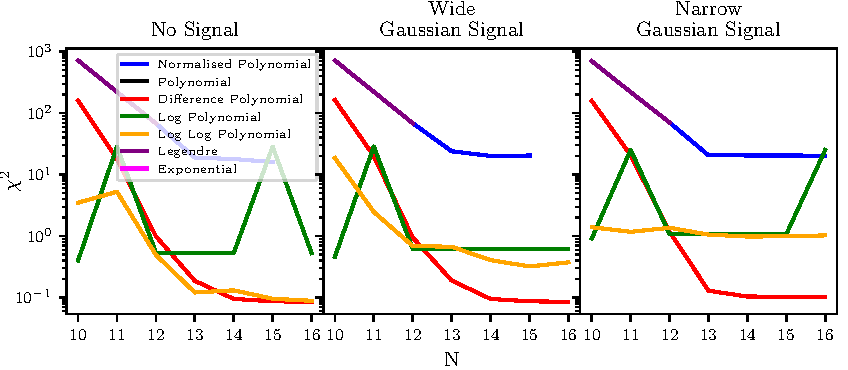
\includegraphics{maxsmooth/figs/Fig9_basis.pdf}
    \caption{A comparison of the quality of MSF fit produced using the sign navigating algorithm and the different built-in \maxsmooth~basis as a function of order $N$ for three mock 21-cm experiment data sets with no signal, a wide Gaussian signal and a narrow Gaussian signal. The Difference Polynomial model, \cref{eq:additional_basis_b} of order $N = 15$ is shown to be the optimal model for fitting these data sets. Beyond $N = 15$ the quality of fit does not improve any further and additional terms in the model have coefficients $a_{k \geq 14} \approx 0$.}
    \label{fig:fig9_bestbasis}
\end{figure*}

\begin{figure*}
    \centering
    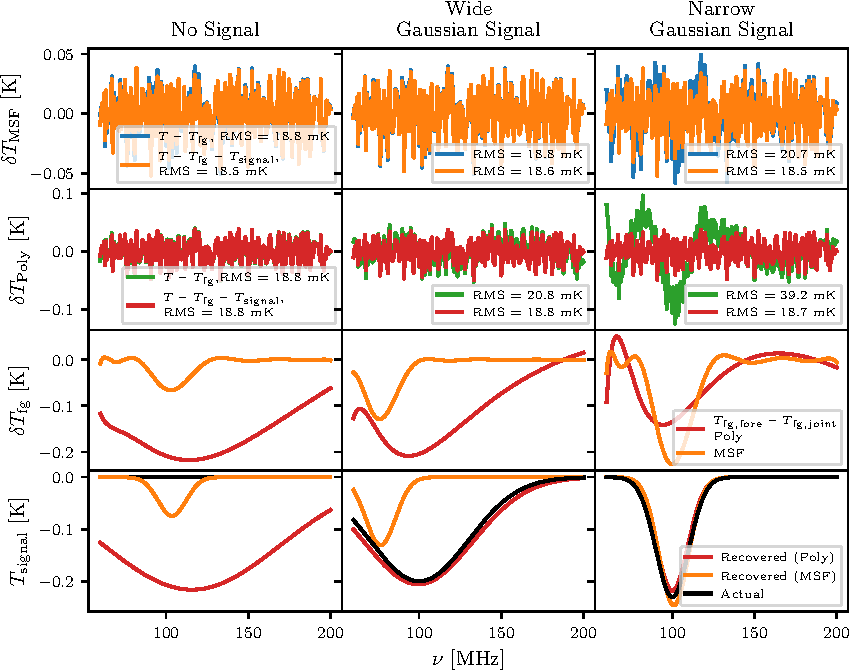
\includegraphics{maxsmooth/figs/Figure9.pdf}
    \caption{The top row shows the resultant residuals when using an MSF to fit just a foreground and to jointly fit a foreground and Gaussian signal model to three mock data sets with no signal, a wide Gaussian signal and a narrow Gaussian signal from left to right. The second row shows the equivalent for an unconstrained polynomial fit. The third row shows the change in foreground, $\delta T_\mathrm{fg}$, between the pure foreground fit, $T_\mathrm{fg, fore}$, and joint fit, $T_\mathrm{fg, joint}$, for both foreground models and all three signal models. The bottom row shows the recovered signals for both foreground models alongside the true signal models in the data sets. The figure appears to show that unconstrained polynomials are better behaved than MSFs, however we would note that the signal models used here are simplistic in nature. We would expect the signals to be more complex, including emission, as with those used in \cref{fig:PSF_comp} for which we showed the use of DCFs to be advantageous.}
    \label{fig:smooth_gauss}
\end{figure*}

For 21-cm cosmology, it is also important to consider how the global 21-cm signal is modelled when performing joint fits. Typically, the signal is modelled as a Gaussian, flattened Gaussian or using physically motivated models. If a Gaussian model is jointly fit with a DCF foreground, then the fit is biased towards returning a `smooth' Gaussian signal with a large width, $\sigma$, even if such a signal is not real. Similarly, incorrectly constrained DCFs can fit out `smooth' signals in data sets. This can cause uncertainty in the presence of such signals, and the point is furthered in \cref{sec:EDGES_fits}.

We can illustrate this by generating three different data sets, all with foregrounds following $\nu^{-2.5}$ and the same Gaussian noise with a standard deviation of $20$~mK. Into two of the three data sets, we add mock Gaussian signals with central frequencies $\nu_c = 100$~MHz and generated using
\begin{equation}
    T_{21} = -A \exp\bigg(-\frac{(\nu - \nu_c)^2}{2\sigma^2}\bigg),
\end{equation}
where $A$ is the amplitude. The first mock signal has an amplitude of $200$~mK and a variance of $30$~MHz representing a realistic wide or smooth Gaussian 21-cm signal. The second represents a narrow Gaussian signal with an amplitude of $230$~mK and a variance of $10$~MHz. The final data set has no additional signal in the band of $60 - 200$~MHz.

\begin{table*}
    \centering
    \begin{tabular}{cccccc}
        \hline
          Model& $(\delta T_\mathrm{fg} - T_\mathrm{sig})_\mathrm{max}$ & $\Delta RMS$ & $\log(Z_\mathrm{fore})$ & $\log(Z_\mathrm{joint})$ & $\Delta \log(Z)$\\
          & [mK] & [mK] \\
         \hline
         \multicolumn{6}{c}{No Signal}\\
         \hline
         MSF & 6.6 &  0.2 & 606.42 $\pm$ 0.03 & 606.85 $\pm$ 0.03 & 0.08 $\pm$ 0.04\\
         Poly & 4.5 &  0.1 & 604.28 $\pm$ 0.03 & 603.38 $\pm$ 0.03 & 0.51 $\pm$ 0.04\\
         \hline
         \multicolumn{6}{c}{Wide Gaussian Signal}\\
         \hline
         MSF & 6.0 &  0.2 & 606.46 $\pm$ 0.03 & 606.57 $\pm$ 0.03 & 0.17 $\pm$ 0.04\\
         Poly & 17.5 &  2.6 & 575.02 $\pm$ 0.03 & 597.85 $\pm$ 0.05 & 22.98 $\pm$ 0.05\\
         \hline
         \multicolumn{6}{c}{Narrow Gaussian Signal}\\
         \hline
         MSF & 18.4 & 1.7 & 588.40 $\pm$ 0.03 & 593.42 $\pm$ 0.05 & 7.44 $\pm$ 0.06\\
         Poly & 81.4 & 20.3 & 432.69 $\pm$ 0.03 & 589.88 $\pm$ 0.06 & 157.10 $\pm$ 0.07\\
    \end{tabular}
    \caption{The table shows the average, across 10 repeats with different random noise, maximum difference between the recovered signals and the change in foreground for the polynomial and MSF pure foreground and joint fits, $(\delta T_\mathrm{fg} - T_\mathrm{sig})_\mathrm{max}$, to the three simulated 21-cm experiment data sets with no signal, a wide signal and a narrow Gaussian signal. Also shown are the average changes in RMS, $\Delta RMS$, between the pure foreground and joint fits for both foreground models and all three data sets. We also provide weighted average log-evidences and values for the change in log-evidence, $\Delta \log(Z)$, between the joint and pure foreground fits with errors calculated from the error in each recovered $\log(Z)$. The comparatively large change in log-evidence for the narrow Gaussian signal data set when using MSFs provides confidence that the recovered signal is truly present in the data. Unconstrained polynomials appear to perform better than MSFs in this analysis. However, the signals used here are simplistic, and we have shown in \cref{fig:PSF_comp} that DCFs behave far better for complex theoretically motivated signals that include emission.}
    \label{tab:gauss_summary}
\end{table*}

We assess the best basis from the \maxsmooth~library for fitting these data sets, and this is shown in \cref{fig:fig9_bestbasis}. The graph shows the minimum $\chi^2$ values when fitting MSFs of a particular form, detailed in the legend, using the \maxsmooth~sign navigating algorithm with a given order $N$ to the three data sets. We find that for all three data sets the best basis choice is the Difference polynomial, \cref{eq:additional_basis_b}, with order $N = 15$. We consequently proceed to fit each data set with this MSF model. We compare the resultant residuals for each data set to those from a joint fit of an MSF, of the same functional form, and a Gaussian 21-cm signal model. We perform the joint fits by using \maxsmooth~with the Python implementation of the Nested Sampling software \multinest~\citep[][]{PyMultiNest,multinest_2008,multinest_2009, multinest_2019}. Here, \multinest~estimates the Gaussian signal parameters, \maxsmooth~fits the foreground model to the data minus the estimated Gaussian signal at each iteration and \multinest~minimises the data minus the foreground model plus the signal model. We also perform the equivalent fits with a 5\textsuperscript{th} order unconstrained polynomial, given by \cref{eq:loglog_poly} using a Lavenberg-Marquardt \citep{Levenberg1944, Marquardt1963} algorithm in place of \maxsmooth. We perform this analysis ten times, generating a new noise distribution each time. An example result is shown in \cref{fig:smooth_gauss} where we have provided the same theoretically motivated priors on all the Gaussian 21-cm models. Respectively from top to bottom the rows in \cref{fig:smooth_gauss} show the residuals after just an MSF fit and after a joint fit for comparison, the equivalent for the unconstrained polynomial fits, the change in foreground between the foreground fit and the joint fit and the recovered signal in comparison to the actual signal. The columns correspond to the case of no signal, a wide Gaussian signal and a narrow Gaussian signal from left to right.

We can see that in the absence of a signal jointly fitting with a Gaussian model and MSF returns an absorption trough. This recovered absorption trough is approximately the same as the change in the foreground model when fitting with just an MSF and the change in the RMS is small. This is illustrated in \cref{tab:gauss_summary} which shows the average results across the ten repeats of this analysis. If this were a real experiment, the fitted model could easily be misinterpreted as a real signal that had been fitted out as part of the foreground model. However, there is a very small change in log-evidence between the pure foreground and joint fit, which would suggest that the signal is not truly present in the data.

In \cref{tab:gauss_summary} the values for the log-evidence for each fit and the change in log-evidence, $\Delta \log(Z)$, between the foreground and joint fits for each data set and each foreground model are reported. While \multinest~returns a log-evidence for the joint fits, \maxsmooth~is not a Bayesian algorithm. However, assuming a Gaussian likelihood, we can use \multinest~to calculate the evidence for our pure foreground fits by having it estimate the noise and calculate the likelihood.

When jointly fitting in the presence of a wide Gaussian signal with an MSF we see a similar result to the case with no additional signal, and we could not confidently say that the signal is present in the data if we had no prior knowledge. In fact, the joint fit has recovered a poor representation of the Gaussian signal because the smooth signal in both instances, pure foreground fit and joint, has been absorbed in the foreground modelling.

Finally, we see that in the case of a narrow Gaussian signal in the data set with an MSF we get an almost exact recovery after a joint fit. There is a larger discrepancy between the difference in foreground models and the recovered signal, as shown in \cref{tab:gauss_summary}, and the reduction in RMS is more significant, giving us confidence that the signal is truly present. Importantly, the change in log-evidence is much larger than in the other two cases, indicating the presence of the signal.

For the unconstrained polynomial, in the case where there is no signal in the data, we appear to recover a very smooth Gaussian signal. However, again the change in log-evidence between the pure foreground fit and the joint fit tells us that neither scenario is more likely, and consequently we would conclude that the signal is not present. For the other two cases, the unconstrained polynomial behaves well. However, we note that the signals induced here are simplistic representations of a global 21-cm signal. We would expect the signal to have a much more complicated structure including emission at high frequencies and similar to the signals used in \cref{fig:PSF_comp} for which we showed DCFs to be advantageous.

When attempting to identify the wide Gaussian signal using DCFs, we also note it will be advantageous to fit using a CSF with derivatives of order $m \geq 1$ constrained. For 21-cm cosmology, we find that CSFs and MSFs are generally equivalent. However, in this case the only significant non-smooth structure in the signal, aside from the inflection point, is the turning point and where an MSF may fit this out a CSF will not.

The problem of identifying and misidentifying smooth signals becomes even more prominent, particularly in the absence of any signal in the data, when modelling the foreground with a DCF in $T - \log(\nu)$ space. Here the sample rate is non-uniform and higher at higher $\log(\nu)$. This makes the problem harder to fit in this region and also `smooths' any signals present at low $\log(\nu)$. Together, these effects can make it difficult to detect signals that can already be considered `smooth' in linear space. Similarly, in the absence of any signal in the data, when jointly fitting with a Gaussian signal model and large prior ranges, the routine estimating the Gaussian parameters will tend to favour `smooth' signals at high frequencies in linear space because of the non-uniformity of sampling in logarithmic space.

\subsection{MSFs and the EDGES Data}
\label{sec:EDGES_fits}

In 2018 the EDGES team reported the detection of an absorption trough at $78$~MHz which could be interpreted as a global 21-cm signal \citep[]{Bowman_edges_2018}. The reported signal is $\approx 2$ times the maximum magnitude predicted by current cosmological models \citep[]{Cohen_global_2017}, and, in order to explain the signal as a 21-cm signal, interactions between dark matter and baryons \citep{Barkana_DM_2018, Barkana_DM_2018, KovetzDM2018, MunozDM2018, SlatyerDM2018} or a higher radio background \citep{Bowman_edges_2018, EwallRB2018, FengRB2018, JanaRB2018, Fialkov2019, MirochaRB2019} are needed.

\begin{figure}
    \centering
    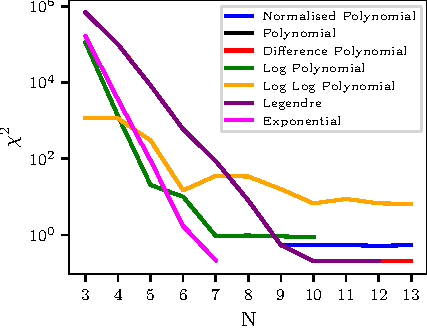
\includegraphics{maxsmooth/figs/Figure10.pdf}
    \caption{The resultant $\chi^2$ as a function of MSF order, $N$, for the \maxsmooth~built-in basis functions fitted to the EDGES data using the \maxsmooth~sign navigating algorithm. The Legendre, Difference polynomial, the Polynomial and Normalised Polynomial models lie on top of each other in this figure. The occasional increase in $\chi^2$ with $N$ for the logarithmic model is because this basis is increasingly unstable with higher $N$ and requires all sign combinations to be tested.}
    \label{fig:EDGES_basis}
\end{figure}

While a higher radio background has been suggested by the results of the ARCADE2 experiment \citep{fixsen_arcade_2011} and potentially confirmed by measurements from LWA \citep{dowell_radio_2018} there are concerns about the analysis of the EDGES data \citep{Hills2018, Sims2020, Singh_edges_2019}. These studies and the following work presented here use the publicly available integrated spectrum from the EDGES Low Band experiment, which can be found at: \url{https://loco.lab.asu.edu/edges/edges-data-release/}.

\begin{figure*}
    \centering
    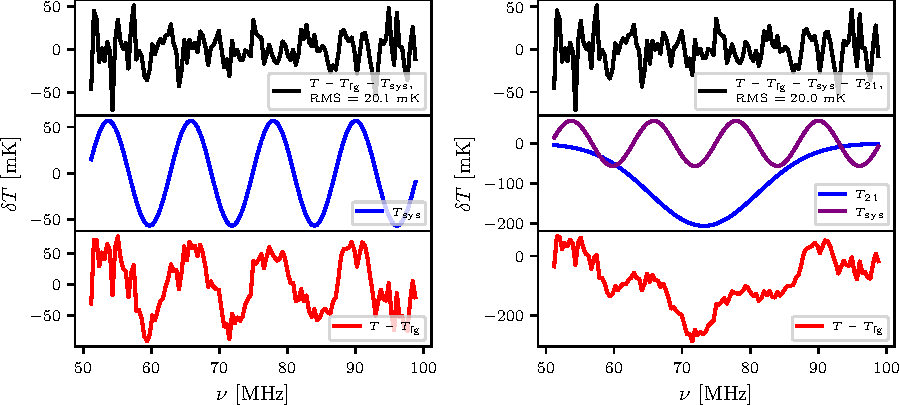
\includegraphics{maxsmooth/figs/Figure11.pdf}
    \caption{\textbf{Left:} The residuals with an RMS of $20.1$~mK and log-evidence of $302.99\pm0.08$, black, found after subtracting from the EDGES data a jointly fit MSF and a sinusoidal systematic. We recover a parameterisation of the systematic, shown in blue, that is consistent with previous work as discussed in the text. The red line, bottom panel, illustrates the residuals after just removing the fitted foreground from the data. \textbf{Right:} A joint fit of a Gaussian 21-cm model signal with a sinusoidal systematic and an MSF foreground to the EDGES data. The recovered 21-cm signal is smooth and the addition of the signal model has caused a large change in the recovered foreground, $T_\mathrm{fg}$, illustrated by the decreased amplitude in the bottom panel around $70$~MHz when compared to that in the left figure. The RMS, $20.0$~mK, is also similar in magnitude to that found for the fit in the left panel and the log-evidence has reduced to $292.67\pm0.17$. Consequently, it is unlikely the model signal is real, and it is probable that it is produced artificially by the change in foreground.}
    \label{fig:EDGES_fits}
\end{figure*}

In \cite{Hills2018} the authors found that recovering the absorption profile using the `physically motivated' foreground model in \cite{Bowman_edges_2018} produces unphysical negative values for the ionospheric electron temperature and optical depth. This suggests that the treatment of the foreground in \cite{Bowman_edges_2018} absorbs part of an unknown systematic. It was also found that a large change in foreground was needed when just fitting a `physical' foreground to the data and when jointly fitting with a flattened Gaussian 21-cm signal profile. In \cite{Hills2018} the authors identify the potential presence of a sinusoidal function in the EDGES data with an amplitude of $\approx 60$~mK and a period of $\approx 12.5$~MHz.

The authors of \cite{Sims2020} fitted a range of models to the EDGES data, varying the 21-cm models between a Gaussian model, a flattened Gaussian model as used by \cite{Bowman_edges_2018} and physical simulations from the ARES code \citep{ARES_sim}. They vary the unconstrained polynomial order for the foreground model and examine likelihoods with and without an additional noise term and a damped sinusoidal function. They use Bayesian Evidence to quantify the most likely scenarios of an atlas of 128 models. The 21 highest evidence models all feature damped sinusoidal functions, all with a consistent amplitude of $\approx~60$~mK and a period of $\approx~12.5$~MHz.

An MSF fit to the foreground should leave a periodic sinusoidal function behind in the residuals if it is present because it is non-smooth in nature. This has previously been shown to be the case by \cite{Singh_edges_2019}, hereafter S19, who identified a sinusoidal feature with an amplitude of $60 \pm 10$~mK and a period of $12.3 \pm 0.1$~MHz. We attempt here to re-create this analysis to validate the \maxsmooth~algorithm. The fitting routine used and choice of basis function are the only differences between the results presented here and in S19. The use of \maxsmooth~means that our joint fit of the data and a systematic model will be computationally quicker and more reliable than the Nelder-Mead based approach to fitting taken in S19, as demonstrated in \cref{sec:Eff}.

We begin first by assessing the quality of fits using the various basis functions built-in to \maxsmooth. S19 used a basis function constrained in $T - \log_{10}(\nu)$ space and although the functional form is not explicitly stated in S19 it is derived from the models in \cite{Sathyanarayana_msf_2017} and so is similar to, if not identical to, \cref{eq:log_poly}. \cref{fig:EDGES_basis} shows the resultant $\chi^2$ as a function of MSF order for fits with varying basis functions using \maxsmooth. %This figure again shows how the choice of basis function can affect the quality of the fit. 
Our $T - \log_{10}(\nu)$ space model cannot achieve the same RMS as that found by S19 with a similar model. With an $N = 7$ MSF constrained in logarithmic frequency space, S19 return an RMS of $44$~mK, whereas with \cref{eq:log_poly} \maxsmooth~returns an RMS of $87$~mK. We believe this is due to the lack of normalisation in \maxsmooth~and as previously discussed this is an ongoing area of development.

We use \cref{fig:EDGES_basis} to inform our choice of basis function and MSF order, and proceed using an 11\textsuperscript{th} order MSF of the form given by \cref{eq:additional_basis_b}. We find residuals with an RMS of $\approx~40.4$~mK and a log-evidence of $216.80\pm 0.09$ as shown in \cref{fig:fig0}. We note that this is in approximate agreement to results shown in S19. We also find troughs at $\approx~70$~MHz and $\approx~85$~MHz which correspond to those found in all the reported sinusoidal functions.

We jointly fit the data with an 11\textsuperscript{th} order MSF and a sinusoidal function of the form
\begin{equation}
    T_\mathrm{sys}~=~p_0~\sin(p_1~\nu~-~p_2),
    \label{eq:sine_sys}
\end{equation}
and the resultant residuals are shown in the left panel of \cref{fig:EDGES_fits}. We have not included a model 21-cm signal in this fit. We use \maxsmooth~along with a Lavenberg-Marquardt algorithm implemented with \scipy~to perform this joint fit and with initial parameters of $p_0 = 60$~mK, $p_1\approx (2\pi)/12.5$~MHz$^{-1}$ and $p_2 = 0$~rad. We find that the results change with the initial parameters when using the Lavenberg-Marquardt algorithm, however, the chosen initial parameters are well-informed by the previous work outlined above. We return parameters of $p_0 \approx 56.6$~mK, $p_1 \approx 0.52~\textnormal{MHz}^{-1}$ or a period of $ \approx 12.1$~MHz and $p_2 \approx 1.1$~rad in close agreement with previous analysis. We use \multinest~to approximate the evidence for this fit, assuming a Gaussian likelihood and return $\log(Z)=302.99\pm0.08$. This is a significant increase in log-evidence when compared to the pure foreground fit and would suggest strongly that the systematic is present in the data.

We find an RMS value of $20.1$~mK, in close agreement with the result of $22.9$~mK found in S19 when jointly fitting an MSF and the sinusoidal function. However, the RMS of the joint fit in the left panel of \cref{fig:EDGES_fits} is equivalent to the RMS found by S19 when jointly fitting an MSF foreground, a sinusoidal systematic and Gaussian 21-cm signal model. Their proposed Gaussian 21-cm signal model fits with standard predictions. However, the RMS of our joint fit without a Gaussian signal model may highlight some of the difficulties in detecting `smooth' Gaussian signals discussed in \cref{sec:limitations}.

We perform a joint fit of a Gaussian 21-cm signal, a sinusoidal systematic and MSF. Due to the increased complexity of the fit and uncertainty in the fit parameters for the Gaussian model, we perform our fit using \maxsmooth~and \multinest. We provide prior ranges of $30 - 80$~mK for the amplitude, $0 - 25$~MHz for the period and $0 - 2\pi$ for the phase shift of the sinusoidal systematic. For our Gaussian we set realistic priors on the amplitude of $0 - 250$~mK, on the central frequency of $50 - 100$~MHz and on $\sigma$ of $0 - 20$~MHz. For the sinusoid we find an amplitude of $56.5$~mK, a period of approximately $12.1$~MHz and a phase of $1.1$~rad. %These results, using a more extensive search of the parameter space, are consistent with our previously result further indicating that when performing the fit shown in the left panel of \cref{fig:EDGES_fits} our initial parameters were well-chosen. 
We return an amplitude of $206$~mK for the Gaussian with a central frequency of $73$~MHz and a $\mathrm{FWHM} \approx 18$~MHz. \multinest~returns a noise parameter of $20$~mK and our resultant fit, shown in the right panel of \cref{fig:EDGES_fits}, has an RMS of approximately $20.0$~mK. This is much wider and deeper than the signal reported in \cite{Singh_edges_2019} which has a depth of $133 \pm 60$~mK and FWHM of $9 \pm 3$~MHz however we return the same central frequency of $73$~MHz.

Noting the discussion of plausibly detectable 21-cm signals when using DCFs and the bias towards `detection' of `smooth' Gaussian signals in \cref{sec:limitations} we assess the feasibility of the returned model signal. Here, the notion of `smoothness' is relative to the bandwidth. In \cref{sec:limitations} a Gaussian with $\mathrm{FWHM} \approx 24$~MHz is confidently identifiable as a real signal, but the bandwidth is much larger than that for the EDGES data. We can see by comparison of the bottom panels of \cref{fig:EDGES_fits}, showing the data minus the foreground from the joint fits, that there is a large change in foreground when we include the Gaussian model as part of our joint fit. This may be because in our initial fit, without the Gaussian model, the foreground model was fitting out the smooth signal. Alternatively, the signal may not be present, and the fitting routine has returned a smooth signal by extracting it from the foreground component of the data. The reduction in RMS when the joint fit includes a Gaussian is negligible, and it is consequently challenging to determine whether the signal is present in the data. However, we can conclude from the log-evidence, which for this fit has a value of $292.67\pm0.17$ and is smaller than that for the joint fit of the systematic and foreground, that the Gaussian is not likely to be real.

\subsection{MSFs and the LEDA Data}
\label{sec:LEDA_fits}

LEDA, like EDGES, is a global 21-cm experiment analysing the band $30 - 88$~MHz and aiming to detect the anticipated absorption feature \cite{Greenhill2012}. The design and calibration approach of LEDA is detailed in \cite{Price_LEDA_2018}. In contrast to EDGES, the LEDA experiment comprises 5 dual-polarization radiometer antennas that are part of a larger 256-antenna interferometric array. This approach is intended to allow inter-antenna comparison and in-situ measurement of the antenna gain response. Similar to other experiments with absolute calibration, LEDA uses two noise diode references to calibrate the measured antenna temperature into units of Kelvin. Corrections are then applied to account for the impedance of the antenna and receiver, derived from vector network analyser~(VNA) measurements. 

As shown in \cite{Price_LEDA_2018}, data are seen to vary between antennas, which are not perfectly identical, and this is attributed to minor differences in terrain, analogue component response, and physical construction. While calibrated spectra are presented, it is suggested that there are unidentified systematics in the data; work has been undertaken to better characterize and update the LEDA system with iterative improvements. %Further measurements were taken in 2017 and 2018, which are under analysis. % (Gardsen et al., in prep.). 

Here, we fit MSFs to data from the LEDA 2016 campaign \cite{Price_LEDA_2018}. This is the first time MSFs have been applied to LEDA data. Specifically, we fit data from antenna 252A, taken on January 26\textsuperscript{th} 2016 in the Local Sidereal Time~(LST) range 11:00-12:00.  In this LST range, the Galactic contribution to the antenna temperature is at a minimum. The data are binned into 1.008 MHz channels, spanning 40--85 MHz.

\begin{figure}
    \centering
    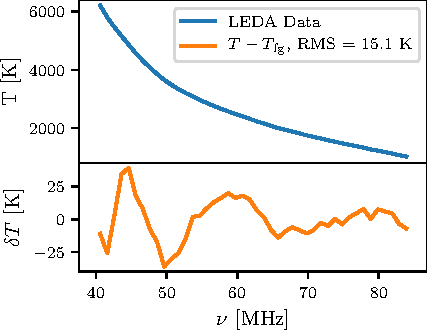
\includegraphics{maxsmooth/figs/Figure12.pdf}
    \caption{The LEDA data from antenna 252A taken in 2016 and averaged over 1 hour of LST shown in the top panel. Also shown, bottom panel, are the residuals after fitting the LEDA data with a 9\textsuperscript{th} order MSF of the form given in \cref{eq:additional_basis_b} with a log-evidence of $-185.45\pm0.09$. We see evidence of a damped sinusoidal systematic in the data set.}
    \label{fig:LEDA_data}
\end{figure}

We fit an MSF of the form given in \cref{eq:additional_basis_b} to the data, as we find that this basis function returns the best fit consistently for $N \geq 8$. Shown in \cref{fig:LEDA_data} are the resultant residuals from an $N = 9$ MSF fit with an RMS of $\approx 15$~K and a log-evidence of $-185.45\pm0.09$. The resultant residuals are large and would obscure a cosmological 21-cm signal. We note that as per equation~(4) in \cite{Price_LEDA_2018} the radiometer noise is expected to be $\approx 0.5$~K.

\begin{figure*}
    \centering
    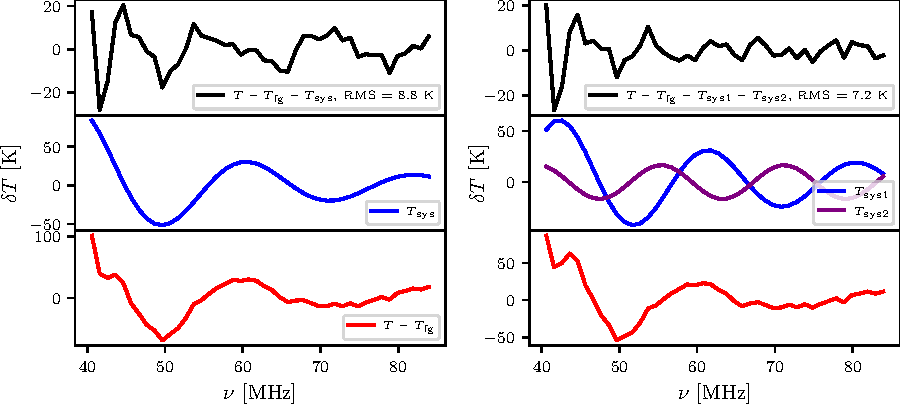
\includegraphics{maxsmooth/figs/Figure13.pdf}
    \caption{\textbf{Left:} The residuals, black, after jointly fitting the LEDA data with an MSF and damped sinusoidal systematic with a log-evidence of $-175.50\pm0.19$. The centre panel shows the recovered systematic model, blue, and the bottom panel shows the residuals, red, after just subtracting the fitted foreground model from the data. The addition of the systematic model has reduced the RMS of the fit when compared to \cref{fig:LEDA_data}. \textbf{Right:} The resultant residuals, black, with a log-evidence of $-168\pm0.19$ found when fitting the LEDA data with an MSF foreground, damped sinusoidal, blue, and additional sinusoidal systematic, purple. Again the bottom panel shows the residuals, red, after just subtracting the fitted foreground model from the data. The further reduction in RMS and increase in log-evidence suggests that both these systematics are present in the data, and indicates that the larger systematics in the LEDA data may be represented by the leading order terms in a damped Fourier series.}
    \label{fig:LEDA_resid}
\end{figure*}

The residuals from the MSF fit appear to include a damped sinusoidal systematic structure. We proceed to fit such a systematic model given by
\begin{equation}
    T_\mathrm{sys}~=~\bigg(\frac{\nu}{\nu_0}\bigg)^{-p_0} p_1~\sin(p_2~\nu~-~p_3),
    \label{eq:damp_sine_sys}
\end{equation}
along with a 9\textsuperscript{th} order MSF by using \maxsmooth~and \multinest. $\nu_0$ is chosen to be the central frequency of the band. We provide a prior on the power of $0 - 3$ for weak damping. Prior ranges of $25~-~75$~K for the amplitude of the sinusoidal function, $0~-~1$~MHz$^{-1}$ for the period, $P$, which is fitted as $p_2=(2\pi)/P$, $0~-~2\pi$ for the phase shift and a log uniform prior on the noise of $10^{-2}~-~10^{1}$~K are also provided. The results of this fit are shown in the left panel of \cref{fig:LEDA_resid}. We return optimal parameters of an exponent of $\approx 2.7$, an amplitude of $\approx 27.9$~K, a period of $21.7$~MHz and a phase shift of $3.7$~rad. The residuals have an RMS of $\approx 8.8$~K and \multinest~returns a noise parameter of $\approx 7.7$~K. We also see an increase in log-evidence, which has a value of $-175.50\pm0.19$, when compared to the pure foreground fit suggesting the systematic is present in the data.

\cite{Price_LEDA_2018} suggest, from analysis of the 2016 LEDA data, that the systematic in the data is caused by the direction-dependent gain of the antenna. A frequency dependent group delay may also be caused by a bandpass filter that could contribute unaccounted for reflections. The pattern of oscillations that form the systematic have also been found to change after rainfall. This systematic may then be caused by moisture in the surrounding soil or by changes in the electric length of the dipoles caused by moisture on the dipole itself. We also highlight the similarities in structure of the systematic with that in the EDGES data. Both have sinusoidal structures, and so similarities between the experimental setups and calibration processes may hint at larger causes of systematics across 21-cm cosmology experiments. The systematic is not likely to be associated with the sky because of the difference in periodicity and amplitude found by both experiments. EDGES does not have a bandpass filter, however it could still be affected by moisture in the surrounding environment. Although we note that this experiment is in a typically dry location~(Murchison Radio-astronomy Observatory, Australia). 

The residuals shown in the top left panel of \cref{fig:LEDA_resid} show a further sinusoidal structure after removal of the leading order damped sinusoidal systematic. We therefore attempt a joint fit to the data using an MSF foreground, a damped sinusoid and an additional sinusoid described by \cref{eq:sine_sys}. We maintain the same priors on the original damped sinusoidal function and provide a prior of $10-30$~K on the amplitude, $0-1$~MHz$^{-1}$ on the period and $0-2\pi$ on the phase shift of the additional systematic.

We find best fit parameters for the leading damped sinusoid of $\approx 1.8$ for the exponent, $\approx 30$~K for the amplitude, a period of $\approx 19$~MHz and a phase shift of $\approx 6.2$~rad. For the additional sinusoidal systematic we find an amplitude of $\approx 17$~K, a period of $\approx 16$~MHz and a phase shift of $\approx 1.5$~rad. \multinest~returns a noise of $\approx 7.2$~K and the fit shown in the right panel of \cref{fig:LEDA_resid} has an RMS of $\approx 7.2$~K. We find a log-evidence for this fit of $-168.34\pm0.19$.

Distinctions between the two systematics have been made in the middle right panel of \cref{fig:LEDA_resid} for clarity. The RMS of the residuals after removal of these two systematics is still significantly larger than the expected radiometer noise for this experiment, $\approx 0.5$~K. However, the decrease in the RMS when these systematics are included in the fit and increase in log-evidence would suggest that both are present in the data. A further addition of sinusoidal systematics will inevitably reduce the RMS of the residuals, in the same way that the residuals after foreground removal could accurately be described by a Fourier series. Higher order terms in the series would feature smaller periods until the periodicity of the terms matched that of the noise. However, the systematics present in the data may have a form described by the leading order terms in a damped Fourier series representing a series of reflections, for example. We leave more rigorous investigation of the additional oscillatory structure in the residuals, top right panel of \cref{fig:LEDA_resid}, to future work.

\section{Conclusions}
\label{sec:maxsmooth_conclusions}

Derivative Constrained Functions~(DCFs) generally are advantageous for experiments in which the desired signal is masked by higher magnitude smooth signals or foregrounds which follow power laws. DCFs are designed to accurately replicate these power law structures by constraining individual high order derivatives of fitted polynomials. They are particularly useful when the signals of interest are expected to be several orders of magnitude smaller than the foregrounds, similar in magnitude to experimental noise and non-smooth.

We have introduced \maxsmooth~as a fast and robust tool for fitting DCFs and demonstrated its abilities with examples in 21-cm cosmology. The code features an extensible library of example DCF models. Further work into the normalisation of these DCF models for \maxsmooth~is anticipated with the aim to improve the quality of fitting and efficiency of the software.

\maxsmooth~is shown to be $\approx2$ orders of magnitude faster than traditionally used Basinhopping/Nelder-Mead based algorithms \cite{Sathyanarayana_msf_2017}. This is an important improvement when jointly fitting signals, systematics and foregrounds using a Bayesian likelihood loop, as in Nested Sampling \citep{Anstey_REACH_2021}.

\maxsmooth~is also designed to be able to cover the entire available parameter space, unlike a penalised Basinhopping/~Nelder-Mead based routine, by dividing it into discrete parameter spaces based on the different allowed combinations of signs, positive and negative, on the constrained derivatives. The extensive exploration of the parameter space provides confidence in the results and the employment of quadratic programming, a robust method for solving constrained optimisation problems, allows \maxsmooth~to remain an efficient algorithm.

We have reproduced analysis of the EDGES data using \maxsmooth~and analysed data from the LEDA experiment with MSFs for the first time. We have highlighted limitations of DCFs when jointly fitting for 21-cm signals and illustrated this using the EDGES data. %We have shown that in the presence of a smooth signal or no signal that DCFs can incorrectly recover signals that are smooth across the band when jointly fitted with signal models. However, this is not a problem that is unique to DCFs, and we have illustrated that it is of equal prevalence when using unconstrained polynomials. 

We show that MSFs preserve turning points of 21-cm signals more consistently than commonly used low order logarithmic unconstrained polynomial models. This is particularly true of 21-cm signals that exhibit significant non-smooth structure in the frequency band of our experiments.% with maximum brightness temperatures, $T_\mathrm{max} \geq 0$~mK and minimum temperatures, $T_\mathrm{min} \geq -225$~mK which feature the strongest deviations, a distinct absorption trough and emission above the background CMB, from the smooth foreground approximated by a $\nu^{-2.5}$ power law. A more detailed exploration of the signal parameter space is needed to fully understand the types of `detectable' or reproducible 21-cm signals when using DCFs with varying constraints to model the foreground.

%We suggest here that DCFs may also be used as a tool for identifying low level RFI, weak spectral lines and, as illustrated for MSFs by \cite{Sathyanarayana2015}, signals from the Epoch of Recombination. In all cases, the signals of interest are non-smooth features masked by higher magnitude smooth signals that can be modelled and removed with DCFs. Applications of DCFs in these fields is left for future work.

We use PSFs and \maxsmooth~in \cref{ch:saras2} to model the foreground structure in data from the SARAS2 instrument.

\begin{comment}
\setcounter{section}{0}
%\renewcommand\thefigure{S.\arabic{figure}}
%\renewcommand\thetable{S.\arabic{table}}
%\renewcommand\thesubsection{S.\arabic{subsection}}
\renewcommand\thesection{\arabic{chapter}.\Alph{section}}

\section{CVXOPT and Quadratic Programming}
\label{app:qp}

Quadratic programs are a special family of convex optimisation problem in which the objective function is quadratic and the conditions are affine in nature \citep[][]{cvx, qp}. \cvxopt~is a Python package for solving a quadratic optimisation problem subject to linear constraints. In \cref{sec:qp} we write the least-squares problem that we are solving in terms of matrices as
\begin{equation}
    \chi^2(\mathbf{a})~=~\frac{1}{2}~\mathbf{a}^T~\mathbf{Q}~\mathbf{a}~+~\mathbf{q}^T~\mathbf{a},
\end{equation}
where
\begin{equation}
    \mathbf{Q}~=~ \mathbf{\Phi}^T~\mathbf{\Phi}~~\textnormal{and}~~ \mathbf{q}^T~=~-\mathbf{y}^T~\mathbf{\Phi},
\end{equation}
subject to a constraint
\begin{equation}
    \mathbf{G}~\mathbf{a}~\le~\mathbf{h}.
    \label{eq:qp_cond}
\end{equation}
This is known as the primal problem when using quadratic programming to solve least-squares. For the constraints on a DCF $\mathbf{h} = \mathbf{0}$.

The problem is solved using the Karush-Kuhn-Tucker~(KKT) theorem \citep[]{KT1951, Karush2014} which re-phrases the above problem in terms of a Lagrangian given in this instance by
\begin{equation}
    \mathbf{L(a,\boldsymbol{\mu})}~=~\chi^2(\mathbf{a})~+~\boldsymbol{\mu^T}\mathbf{g(a)},
\end{equation}
where $\mathbf{g(a)}~=~\mathbf{G~a}-\mathbf{h}$ and $\boldsymbol{\mu}$ is the Lagrange multiplier.

From the Lagrangian we can define the Lagrangian dual function to be
\begin{equation}
    l(\boldsymbol{\mu}) = \min_{x} \mathbf{L(a,\boldsymbol{\mu})},
\end{equation}
which leads to the dual problem minimizing $l(\boldsymbol{\mu})$ subject to $\boldsymbol{\mu} \geq 0$.

The condition on the dual problem that $\boldsymbol{\mu} \geq 0$ is derived from the definition of the condition on the primal problem and the definition of $\mathbf{g(a)}$. The condition is known as complementary slackness and is given by
\begin{equation}
    \boldsymbol{\mu}\mathbf{g}(\mathbf{a})~=~0.
\end{equation}
Since $\mathbf{g}(\mathbf{a})~\le~0$, by definition this implies
\begin{equation}
    \boldsymbol{\mu}~\ge~0.
\end{equation}

The theorem states that if the point given by $(\mathbf{a^*}, \boldsymbol{\mu^*})$ is a saddle point in the Lagrangian in the domain with $\boldsymbol{\mu}~\ge~0$ then $\mathbf{a^*}$ is a solution to the optimisation problem. This is known as strong duality and can be re-phrased as
\begin{equation}
    \chi^2(\mathbf{a^*}) = l(\boldsymbol{\mu^*}).
\end{equation}

By taking the gradient of the Lagrangian and setting this equal to zero, since we are looking for a stationary point, we find
\begin{equation}
    \nabla \chi^2(\mathbf{a^*}) -\sum_i\mu_i^*\nabla g_i(\mathbf{a^*})~=~0,
    \label{eq:lagange_derive}
\end{equation}
where the sum is over the total number of different constraints. An optimal solution of the primal problem will be a stationary point with $\nabla \chi^2(\mathbf{a^*}) = 0$ and consequently we have $\sum_i\mu_i^*\nabla g_i(\mathbf{a^*})~=~0$ by \cref{eq:lagange_derive} leading to the required saddle point.

The algorithm consequently looks for solutions $\mathbf{a^*}$ for which a non-negative $\boldsymbol{\mu^*}$ can be found and the KKT conditions can be satisfied. To summaries the conditions are as follows,
\begin{enumerate}
    \item Stationary Condition: The optimal solution of the prime and dual problems will produce a saddle point in the Lagrangian.
    \item Complementary slackness: $\boldsymbol{\mu^*}\mathbf{g}(\mathbf{a^*})~=~0$  holds.
    \item Primal Feasibility: The condition given by \cref{eq:qp_cond} is satisfied by $\mathbf{a^*}$.
    \item Dual Feasibility: The Lagrangian multiplier satisfies the inequality $\boldsymbol{\mu^*}\geq 0$.
\end{enumerate}

\section{Visualising Constraints in Parameter Space: Alternative Basis}
\label{app:param_space_alt_basis}

\cref{fig:loglog_poly_params} shows the resultant parameter spaces when fitting a 5\textsuperscript{th} order MSF to data of the form $y = x^{-2.5}$ using the logarithmic basis function given by \cref{eq:loglog_poly}. As discussed in \cref{sec:qp} the parameter space presented here is unique to the data set and DCF model used. However, it highlights the importance behind the choice of basis and illustrates the differences in the constraints produced when defining the DCF in a different data spaces.

\begin{figure*}
 \centering
    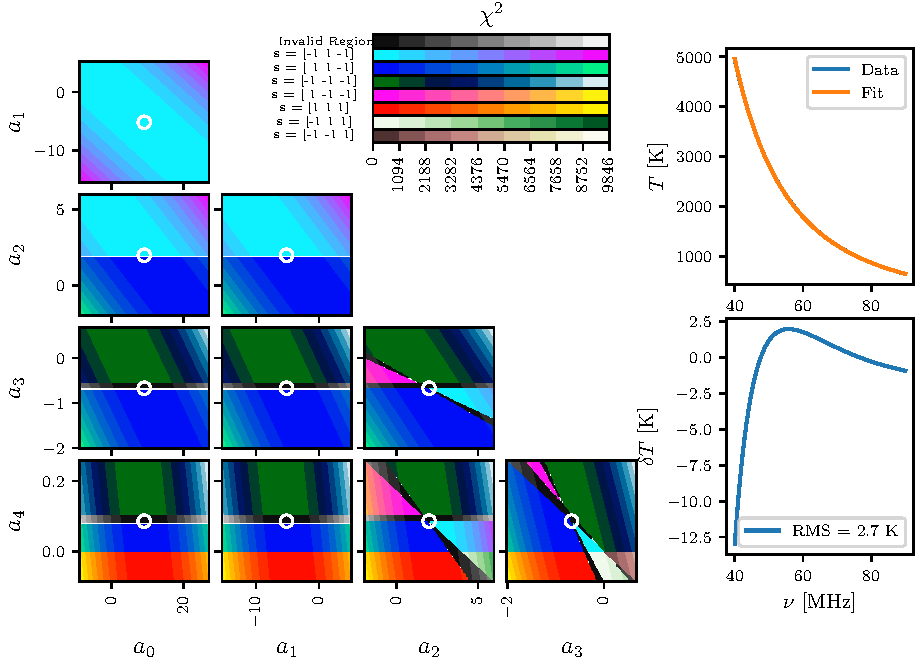
\includegraphics{maxsmooth/figs/FigureB1.pdf}
    \caption{\textbf{Left:} The equivalent of the left panel in \cref{fig:poly_params} using a 5\textsuperscript{th} order MSF of the form given by \cref{eq:loglog_poly} and constrained in $\log_{10}(y) - \log_{10}(x)$ space. As with \cref{fig:poly_params} black regions show regions in which the MSF condition is violated and the coloured regions illustrate sign combinations for which the constraints are upheld. The ranges on the parameters are determined to be $200\%$ on either side of the optimal values from the MSF fit. In each panel two of the parameters are varied while the others are maintained at their optimal values. Here, the regions for which the conditions are violated are narrow and consequently multiple discrete sign spaces are found to produce similar $\chi^2$ values. This strongly suggests that the problem is ill defined and hard to solve using the sign space navigation described in \cref{sec:Eff}. \textbf{Top Right:} The mock 21-cm experiment data and the MSF fit for which the parameter space is analysed. $T$ refers to the averaged sky temperature and $\nu$ to the frequency. \textbf{Bottom Right:} The residuals after subtracting the MSF fit from the data set.}
    \label{fig:loglog_poly_params}
\end{figure*}

\section{Standard Derivative Sign Patterns}
\label{app:derivatives}

In \cref{sec:Eff} we introduce the concept of standard derivative sign patterns for particular polynomial structures. To reiterate and enforce this point \cref{fig:standard_der_patterns} illustrates that the derivatives of a polynomial of the form $y \approx x^k$ are all positive, $y \approx -x^k$ are all negative, $y \approx x^{-k}$ are alternating negative to positive from $m = 1$ and $y \approx -x^{-k}$ are alternating positive to negative from $m = 1$. Since, as discussed in \cref{sec:qp}, \cvxopt~constrains the derivatives, $\mathbf{G}\mathbf{a}$ subject to \cref{eq:cvx_const} we would expect the optimum \maxsmooth~signs for an MSF fit to $y \approx x^k$ to be approximately all negative. Similarly for an MSF fit to a polynomial of the form $y \approx -x^{-k}$ we would expect the optimum signs to be alternating positive to negative for $m \geq 2$.

Note that these standard derivative sign patterns are defined in $y - x$ space. The patterns in $y - z$ space will have similar structures and in logarithmic space they are expected to be different however they will still subscribe to a regular structure.

\begin{figure*}
    \centering
    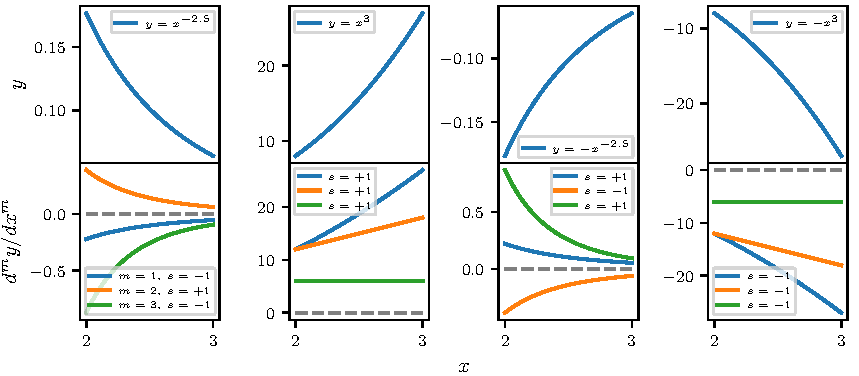
\includegraphics{maxsmooth/figs/FigureC1.pdf}
    \caption{Standard derivative sign patterns associated with four possible standard polynomial data structures. The first row shows example power laws following $y\approx x^{-k}$, $y\approx x^k$, $y\approx -x^{-k}$ and $y\approx -x^k$. The second row shows the derivatives of those power laws up to $m = 3$ and the associated patterns in derivative sign. Note these are not the \maxsmooth~signs and this is discussed in the associated text.}
    \label{fig:standard_der_patterns}
\end{figure*}
\end{comment}

\chapter{\textsc{globalemu}}
\label{ch:globalemu}
\renewcommand\thesection{\arabic{chapter}.\arabic{section}}

\section{Introduction}

To recap \cref{ch:introduction}, the relative magnitude of the features of the 21-cm signal is determined by various astrophysical processes including; the Wouthuysen-Field effect~\citep{Wouthuysen1952, Field1959}, Lyman-$\alpha$ heating and CMB heating \citep{Chuzhoy2007, Venumadhav2018, Villanueva2020, Mittal2021, Reis_sta_2021}, X-ray heating and ionization of the hydrogen gas by UV emission \citep{Madau1997}. %A detailed discussion of the physics describing the global 21-cm signal can be found in \cite{Furlanetto_review_2006}, \cite{Pritchard2012}, \cite{Barkana_review_2016} and \cite{Mesinger2019}. 
The physical processes themselves and hence the global signal can be characterised by a set of astrophysical parameters (see \cref{sec:training_data} and \cite{Cohen2020}): the star formation efficiency, $f_*$, the minimal virial circular velocity, $V_c$, the X-ray efficiency, $f_X$, the CMB optical depth, $\tau$, the slope of the X-ray spectral energy density~(SED), $\alpha$, the low energy cut-off of the X-ray SED, $\nu_\mathrm{min}$, and the mean free path of ionizing photons, $R_\mathrm{mfp}$.

Hybrid approaches are used to calculate realizations of the 21-cm signal, over a large cosmological volume and redshift range, which then can be averaged at every redshift separately to give the global signal \citep[e.g.][]{Mesinger2011, Visbal_2012, Fialkov_rich_2014, Cohen_global_2017, Reis_sta_2021}. Each simulation takes several hours to perform on a desktop \citep{Monsalve_EDGES_HB_3_2019} and though this is much faster than hydrodynamical simulations, this time is too long to allow us to constrain astrophysical parameters using data. Therefore, the desire to emulate the global signal with neural networks, trained on the results of the large scale simulations, has arisen. The neural networks can produce a realisation of the global signal in a fraction of a second by interpolating between the simulated cosmological and astrophysical models. This means they can be used to physically model the signal in, for example, Bayesian Nested Sampling loops\footnote{Note that here we are not referring to a Bayesian Neural Network \citep[see][]{Javid2020} but rather parameter optimisation algorithms such as \textsc{polychord} \citep[see][]{Handley2015a, Handley2015b}.}, as in the REACH data analysis pipeline~\citep{Anstey_REACH_2021}, in which millions of calculations need to be made to infer cosmological parameters~\citep[][Sims et al. 2021 (in prep.)]{Liu2020, List2020, Chatterjee2021}. 

A number of papers have considered emulation of the 21-cm power spectrum using convolutional neural networks and other techniques \citep[e.g. ][]{Schmit2018, Jennings2018, Mondal_LOFAR_2020}. At the time of writing \cmGEM~ is the only publicly available emulator used to accurately, with a maximum normalised Root Mean Square Error~(RMSE) of $10.55$~\%, and quickly (see \cref{timing}) emulate the global 21-cm signal \citep{Cohen2020} \footnote{During review of this work for Monthly Notices of the Royal Astronomical Society a pre-print (now a published paper) describing the global signal emulator \textsc{21cmVAE} was made public \citep{21cmVAE} in which the comparative performance of \name~is discussed.}. It has previously been used to provide constraints on the parameter space of the 21-cm signal using EDGES high-band data \citep{Monsalve_EDGES_HB_3_2019}. The emulator uses Principal Component Analysis~\citep[PCA,][]{Pearson1901}, the seven astrophysical parameters detailed above and in \cref{sec:training_data}, additional information about the mean collapsed fraction of halos as a function of redshift, $f_\mathrm{coll}(z)$, the fraction of X-ray energy above 1 keV, $f_{\mathrm{XR} > 1 \mathrm{keV}}$, and 2 keV, $f_{\mathrm{XR} > 2 \mathrm{keV}}$, and relies on a division of the signal into 2 or 3 distinct segments defined by the turning points. It involves the application of a decision tree for classification and several regression neural networks estimating PCA components, the frequencies and temperatures of turning points as well as additional parameters such as the frequency at which the neutral fraction equals 0.16, $\nu(x_{HI} = 0.16)$.

In this chapter we present \name~which uses a novel and robust approach with a single small scale neural network to emulate the global 21-cm signal given a comprehensive set of astrophysical parameters and redshift range. Where previously \cmGEM~was designed to take in astrophysical parameters and return a low dimensional representation of the global signal as a function of redshift, \name~takes in the same astrophysical parameters and redshift and returns a signal temperature at the corresponding redshift~(see \cref{fig:network_types}). This greatly simplifies the complexity of the relationship being learnt by the neural network. It means we can achieve accurate results, with the smoothness of the signal imposed by the interpolation of the neural network between signals in the training data set, using a small network and without the need for a compressed representation of the signals like PCA where there is a potential loss of information. Additionally, \name~relies on a physically motivated pre-processing of the training data and can emulate a high resolution, $\delta z = 0.1$ over the range $z = 5 - 50$, global 21-cm signal in $\approx1.3$ ms. \name~will be used extensively by the REACH collaboration and has been designed to have an average accuracy less than or equal to 10~\% of the expected noise in the REACH system, estimated to be $\approx25$ mK \cite{de_lera_acedo_reach_2022}.

\name~is written in Python using \texttt{tensorflow} and the \texttt{KERAS} backend, it is pip installable via \texttt{pip install globalemu} and available at \url{https://github.com/htjb/globalemu}. It is flexible enough to be retrained on any set of global 21-cm signal models, whilst maintaining the novel design and physically motivated pre-processing. We provide a demonstration of its accuracy and efficiency in this chapter using the same data used to train \cmGEM~and the corresponding trained models are publicly available on GitHub. We use GitHub actions to perform continuous integration.

In \cref{sec:parameterisation_globalemu} we describe the novel approach used to parameterise \name. \Cref{sec:training_data} describes the training and test data used to illustrate the capabilities of \name~in this chapter and the astrophysical parameters in the simulations of the global signal. We then describe the predominantly physically motivated pre-processing of the inputs and outputs of the neural network in \cref{sec:preprocessing}. A discussion of the neural network structure follows in \cref{structure} and the quality of emulation is assessed in \cref{sec:globalemu_results}. We conclude in \cref{sec:globalemu_conclusions}.

The co-authors, namely Will Handley, Anastasia Fialkov, Eloy de Lera Acedo and Kamran Javid, of \cite{Bevins_globalemu_2021} provided comments and feedback on the original manuscript that this chapter is modified from.

\section{Parameterising the Problem}
\label{sec:parameterisation_globalemu}

There are several approaches that can be used to emulate the global 21-cm signal with a neural network. The ultimate goal of the emulator is to take in a set of astrophysical parameters and return an estimate of the signal brightness temperature as a function of redshift, $T_{21}(z)$, where the relationship has been learned from detailed semi-numerical simulations. This can be done directly with a neural network that returns a value of $T_{21}$ for each redshift data point it has been trained on. However, assuming the network is trained on high resolution signals this would result in a large number of outputs, making it hard to train, and would be limited in predictive power to specific values of redshift. The process can also be achieved by estimating, via a neural network, coefficients of a compressed representation of the signal space. For example, using PCA as with \cmGEM~\citep{Cohen2020} or learning coefficients of basis functions for polynomials or wavelets that when combined return the global signal. However, whilst this approach reduces the number of outputs compared to a direct emulation, if incorrectly designed this can result in information loss and is equally limited in predictive power.

We take the novel approach of using redshift as an input to the network alongside the astrophysical parameters and returning from the network a single corresponding temperature. This is beneficial for two reasons; the small number of inputs and outputs means that the network can retain a simple structure and second the network will be able to interpolate between the values of redshift that it has been trained on. The smooth structure of the output from the network is guaranteed by the smooth interpolation performed by the neural network and by the smooth structure of the signals it is learning. Vectorised calls to the network are used to emulate the temperature as a function of redshift.

In \name~we also provide the ability to emulate the evolution of the neutral fraction, $x_{HI}$, of hydrogen as a function of redshift. We use an identical framework as when emulating the global signal to do this with a set of astrophysical parameters and a redshift as inputs to a neural network and a corresponding value of $x_{HI}$ as an output.

We have built a network that can emulate the global 21-cm signal to a high degree of accuracy without the need for L1 and L2 regularisation, dropout \citep{Srivastava2014}, batch normalisation \citep{Ioffe2015} or other similar concepts. We have achieved this by focusing on the pre-processing of the network's inputs and outputs, with the goal to make the problem simple to solve with a basic neural network of a `reasonable' size.

\begin{figure*}
    \centering
    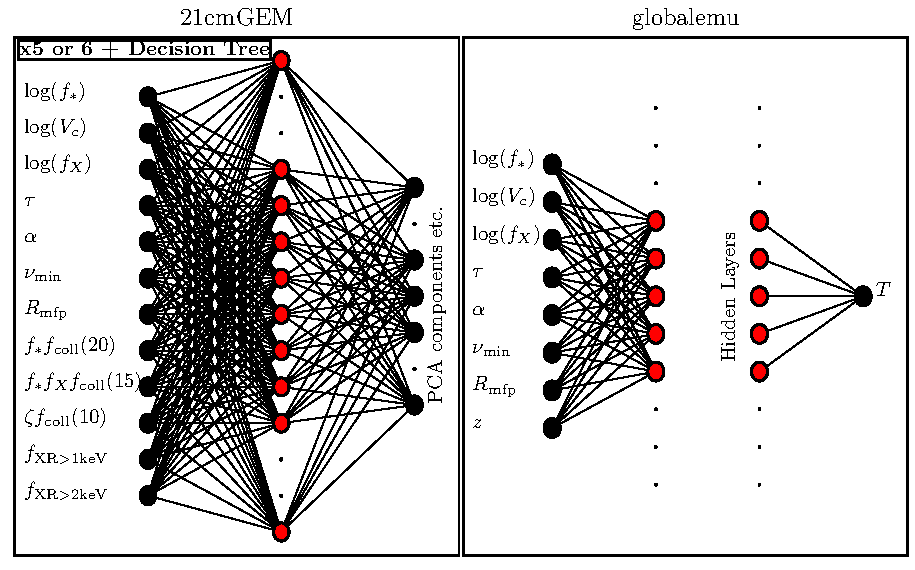
\includegraphics{globalemu/figs/21cmGEM_matplotlib_network_diagram.pdf}
    \caption{\textbf{Left Panel:} We provide here an illustration of the regression neural networks used in \cmGEM. Note that \cmGEM~uses either 5 or 6 of these networks and a decision tree when making predictions.  For one of the regression networks used, the only input parameters are the seven astrophysical parameters detailed in \cref{sec:training_data}~(excluding redshift). However, for the others there are an additional five derived parameters (see text and \protect\cite{Cohen2020}) and we illustrate the full set of 12 inputs. The number of output nodes depends on the specific application of the network, and they can correspond to either PCA components (4 nodes), additional parameters such as $\nu(x_{HI} = 0.16)$ (1 node) and the frequencies and brightness temperatures of turning points in the signal (7 or 5 nodes). The hidden layer in all the \cmGEM~regression networks have 40 nodes. For a full illustration of the \cmGEM~algorithm and detailed description, see Fig. 11 and section 4.2 in \protect\cite{Cohen2020}. \textbf{Right Panel:} An illustration of the \name~neural network. Note the use of only one network to emulate the global signal, in comparison to the 5 or 6 used for \cmGEM. Here the input layer has eight nodes (seven astrophysical parameters plus redshift) and the output layer is a single node returning the brightness temperature corresponding to the input redshift. We show a sizable hidden layer structure here with the red nodes and `...' however, we note that the reduced number of inputs and outputs implies that a small architecture will be sufficient to achieve a high level of accuracy in the emulation~(see \cref{structure}).}
    \label{fig:network_types}
\end{figure*}
    
    
\section{The Training and Test Data}
\label{sec:training_data}

In this chapter, we use the same model signals and corresponding astrophysical parameters used to train and test \cmGEM~\citep[available at \url{https://doi.org/10.5281/zenodo.4541500},][]{Cohen2021Data}. Examples of the global signals from the training set are shown in the left panel of \cref{fig:example_signals}. In total the data set contains 27,292 training models and 2,174 test models with each model being dependent on 7 astrophysical parameters. Each global signal in the data set has 451 redshift data points, and this means that each signal corresponds to 451 training points with the same astrophysical parameters and different redshifts. Therefore, for \name~the 27,292 training models become 12,308,692 training data points. However, we continue throughout this chapter to talk generally of training signals rather than data points because the emulator will be used to determine the signal structure over a redshift range~(see \cref{sec:globalemu_results} for more details).

The data pre-processing is explained in detail in \cref{sec:preprocessing}. Explicitly, the inputs \citep{Cohen_global_2017, Monsalve_EDGES_HB_3_2019, Cohen2020} to the neural network when training on the \cmGEM~data are as follows (ranges are based on those in the \cmGEM~training data set, see section 2.5 of \cite{Cohen2020});
\begin{itemize}
    \item $f_*$: The star formation efficiency takes values in the range $0.0001 - 0.5$ and characterises the amount of gas converted to stars in the dark matter halos. A low star formation rate results in a low Lyman-$\alpha$ flux and late onset of X-ray heating, leading to a shallower absorption trough and weak or non-existent emission above the radio background in the signal.
    \item $V_c$: The minimal virial circular velocity has a value in the range $4.2 - 100$~km/s and is proportional to the cube root of the minimum threshold mass for star formation. A low value of $V_c$ corresponds to a small minimum mass threshold which in turn leads to an earlier onset of Lyman-$\alpha$ coupling, responsible for the absorption feature in the global 21-cm signal, and shifts the minimum of the signal to higher redshifts.
    \item $f_X$: The X-ray efficiency of sources has a range between $0-1000$ and a high value corresponds to a high total X-ray luminosity. This leads to an earlier onset of X-ray heating which also shifts the minimum of the signal to higher redshifts, contributes to a shallower absorption and results in a significant emission feature during reionisation at low redshifts.
    \item $\tau$: The CMB optical depth in the \cmGEM~data sets takes a value in the range $0.04 - 0.2$ and a higher value of $\tau$ corresponds to a higher value of the ionizing efficiency of sources, $\zeta$. For high $\tau$ we would see an earlier reionisation of the hydrogen gas. We note that $\tau$ is given as $0.054 \pm 0.007$ by \cite{Planck2018} and that this falls at the lower end of the range in our training and testing data set. More recent parameter studies have explored lower values of $\tau$ in greater detail \citep{Reis_sta_2021}. However, the \cmGEM~data is sufficient to demonstrate the abilities of \name.
    \item $\alpha$: The power defining the slope of the X-ray Spectral Energy Density~(SED) with a range given by $1-1.5$. The global 21-cm signal is expected to have a very weak dependence on $\alpha$ with the largest effect happening at low redshifts.
    \item $\nu_\mathrm{min}$: The low energy cut-off of the X-ray SED has a range of $0.1-3$~keV. Low values of $\nu_\mathrm{min}$ correspond to a soft X-ray SED, efficient X-ray heating and a weak absorption feature in the 21-cm signal.
    \item $R_\mathrm{mfp}$: The mean free path of ionizing photons, with a range $10-50$~Mpc. $R_\mathrm{mfp}$ is expected to have a very weak effect and only at low redshifts \citep[see e.g. ][]{Monsalve_EDGES_HB_3_2019}. A low $R_\mathrm{mfp}$ corresponds to a slower ionization of the neutral hydrogen gas.
    \item $z$: The redshift of the 21-cm brightness temperature is a measure of time and provides details about when each feature of the signal occurred. For example, the brightness temperature is expected to reach 0~mK, corresponding to the end of the EoR, at low redshifts or more recent times. It is interchangeable with frequency given that the rest frequency, $\nu_r$, of the 21-cm line is 1420~MHz
    \begin{equation}
        z + 1 = \frac{\nu_r}{\nu}.
    \end{equation}
\end{itemize}

To ensure that we make a fair comparison of our results with those found when using \cmGEM~we make the same physically motivated cuts to the test data as are detailed in section 2.4 of \cite{Cohen2020}. This equates to limits on the ionizing efficiency of sources, $\zeta < \zeta_\mathrm{max} = 40,000 f_*$ and on the neutral fraction history at $z = 5.9$, $x_{HI}(z = 5.9) < 0.16$. Respectively, the limits are motivated by stellar models \citep{Bromm2001} and quasar absorption troughs \citep{McGreer2014}. We also note that some of the parameters in the testing data have different ranges and the ranges are as follows; $f_*$: $0.0001 - 0.5$, $V_c$: $4.2 - 76.5$ km/s, $f_X$: $0-10$, $\tau$: $0.055 - 0.1$, $\alpha$: $1 - 1.5$, $\nu_\mathrm{min}$: $0.1 - 3$ keV and $R_\mathrm{mfp}$: $10 - 50$ Mpc. In total, the final testing data set comprises 1703 models.

\name~includes a simple-to-use \textsc{python} graphical user interface~(GUI)\footnote{After installation via \textsc{pip} or from source, the GUI can be called from the terminal using the command \textit{globalemu}. See the documentation at \url{https://globalemu.readthedocs.io/} for more details.} in which the variation of the signal with each of the astrophysical parameters listed above can be explored in more detail.
We note that the GUI is a feature made possible by the speed of emulation when using \name~(see \cref{sec:globalemu_results}).
There is an equivalent GUI for the neutral fraction history emulation.

As previously stated, \name~is not limited to emulating signals modelled with the above astrophysical parameters. It is flexible enough that more complicated astrophysical relationships can also be emulated. For example, one explanation for the unexpected depth of the EDGES absorption trough is the presence of a higher than expected radio background, which can be characterised with a quantity $f_\mathrm{radio}$ determining the normalisation of the radio emissivity~\citep[assuming the source of the excess radio background is stellar,][]{Reis2020}. In \cref{ch:saras2} we train \name~on such models, models with a different model of the excess radio background and standard astrophysical models with updated physics in comparison to the \cmGEM~models. %\name~is in principle capable of being trained on models that consider $f_\mathrm{radio}$ in addition to the above 7 astrophysical parameters and redshift as inputs since it assumes nothing about the astrophysical parameters themselves. Equally \name~could be trained on less complex models.

For the neutral fraction, $x_{HI}$, we use a set of models produced as a by-product of the detailed \cmGEM~global signal simulations. The data set is smaller with 10,047 training models and 791 test models however the relationship between the astrophysical parameters and $x_{HI}$ is expected to be (and shown to be, \cref{sec:globalemu_results}) simpler. We note that for $z \gtrsim 30$ the neutral fraction is expected to always be 1, and so we only emulate the neutral fraction over the range $z=5-30$. The models have not been released publicly, but the parameter ranges are the same for this data set as detailed above. A subsample of the training models are shown in the right panel of \cref{fig:example_signals}.

We note that a non-uniform coverage of the parameter space in the training data set, as with the \cmGEM~global signal and neutral fraction data, may introduce bias in the neural network. The network will tend to learn regions of the astrophysical parameter space where the sampling is heavier better than others. For the purposes of illustrating the accuracy of the emulation in this chapter, this is not an issue. %However, it can become an issue when using an emulator to physically model a signal in a data set where parameter estimation may be biased towards a false set of parameters. 
Training a network on a more uniform data set can alleviate this issue.

\begin{figure}
    \centering
    \begin{subfigure}{.5\textwidth}
    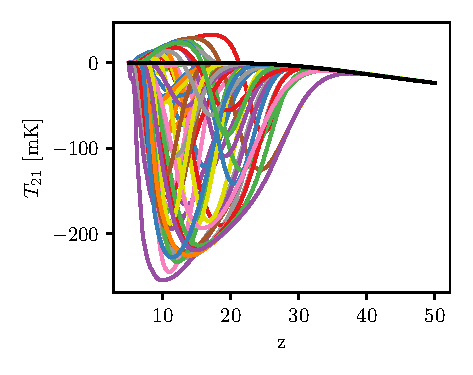
\includegraphics{globalemu/figs/Example_signals.pdf}
    \end{subfigure}%
    \begin{subfigure}{.5\textwidth}
    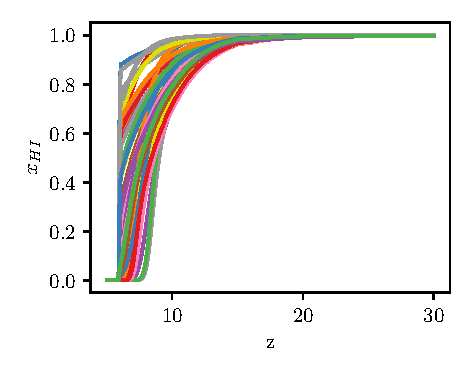
\includegraphics{globalemu/figs/xHI_Example_signals.pdf}
    \end{subfigure}
    \caption{\textbf{Left Panel:} A subsample of 50 global 21-cm signals from the \cmGEM~training set used here to demonstrate the efficiency of \name. The signals show the expected variety of structure, with deep and shallow absorption troughs caused by Lyman-$\alpha$ coupling and terminated by X-ray heating. We also see emission against the CMB background at low redshifts in some of the models where there has been sufficient heating. Also shown in black is the Astrophysics Free Baseline~(AFB) (\cref{sec:afb}) which we model and remove from the training signals before we pass them through the neural network. Subtraction of the AFB prevents our network from attempting to learn a steadily decreasing temperature at high redshifts prior to star formation. \textbf{Right Panel:}A subsample of 50 neutral fraction histories from the training set used in this chapter. At high redshift, the hydrogen in the universe is predominantly neutral and consequently $x_{HI}=1$. As the gas is ionised by UV emission from the first stars, the neutral fraction decreases until $x_{HI}=0$ at the end of the EoR.}
    \label{fig:example_signals}
\end{figure}

\section{Data Pre-processing}
\label{sec:preprocessing}

The details in the following discussion outline the pre-processing for the network predicting the global 21-cm signal. The various pre-processing steps outlined can be switched on and off by a user when training an emulator with \textsc{globalemu}. In \cref{neutral frac pp} we briefly discuss the pre-processing for the neutral fraction networks, which is a largely similar process. The pre-processing is summarised as a flow chart in \cref{fig:flow}.

\begin{figure}
    \centering
    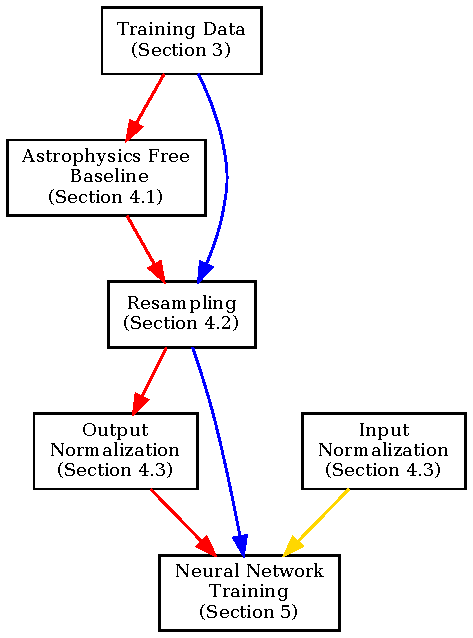
\includegraphics{globalemu/figs/flowchart.pdf}
    \caption{The pre-processing applied to the training data in \name. Each box is outlined in more detail in the corresponding sections. The red path is the pre-processing steps used for the global 21-cm signals, the blue path for the neutral fraction histories and the gold path are steps that occur when training both neural networks.}
    \label{fig:flow}
\end{figure}

\subsection{Astrophysics Free Baseline Subtraction}
\label{sec:afb}

In the region where the structure of the global 21-cm signal is expected to be dominated by collisional coupling, it is independent of the 7 astrophysical parameters used here as inputs to the emulator. This means that, in the corresponding redshift range, each of the signals in our training and testing data sets have the same brightness temperatures. To prevent our network unnecessarily attempting to learn a non-trivial structure in this region, we can treat it as an Astrophysics Free Baseline~(AFB), model and remove it from the signals before they are passed to the network for training. By doing this, our network will learn a simpler relationship at high redshift between the parameters and $T_{21}(z)$ then the existing steadily decreasing trend (see \cref{fig:example_signals}).

In Appendix A in \cite{Bevins_globalemu_2021} we give an approximate calculation of the AFB for the simulated signals that comprise the training data sets. The calculation follows the mean evolution of the signal and in contrast the simulations are produced over large-scale cosmological volumes evolved over cosmological time then averaged. We therefore normalise our result to the temperature of the signals in the training set at $z = 50$ and find that this is sufficient to represent the astrophysics free component of the signals.

As stated, the AFB is then subtracted from the models before training the network and added back in after making predictions.

\cmGEM~uses five extra parameters in addition to the seven astrophysical parameters used here. In principle, these parameters could be passed to the neural network during training due to the flexible nature of \name. However, three of these additional parameters rely on the fraction of mass contained in halos above the minimum cooling threshold, $f_\mathrm{coll}(z)$, and help the network learn the signal structure at high redshift where collisional coupling (cosmology) dominates. Here we do not consider these parameters, which are derived from the seven astrophysical parameters described above, as we are instead removing the AFB. The final two parameters are the fractions of X-ray energy above 1 keV and 2 keV. These parameters are added to further characterise the X-ray SED, but we find with \name~that we do not need to consider them to achieve accurate results.

\subsection{Resampling of signals}

The turning points, and gradients between them, of the global 21-cm signal encode all the information about the efficiency of Lyman-$\alpha$ coupling, X-ray heating and reionization. They are therefore highly dependent on the relevant astrophysical parameters and in the region where the features typically occur variation in the signals is significant. The original signal models are sampled uniformly in redshift, and there is no particular physical motivation for this. However, to improve the quality of modelling we resample the signals at a higher rate across the redshift ranges that typically correspond to the locations of the turning points and at a lower rate where the signal structure deviates less from the `average' signal (e.g. above $z\approx30$ where the signal is free of astrophysics).

To do this we look at the variation in the signal amplitudes, after subtracting the AFB, across the training data set
\begin{equation}
    \Delta T_{21}(z) = T_{21,~\mathrm{max}}(z) - T_{21,~\mathrm{min}}(z),
    \label{eq:resamp-dif}
\end{equation}
and we treat this as a probability distribution
\begin{equation}
    P(\Delta T_{21}(z)) = \frac{\Delta T_{21}(z)}{\sum_z \Delta T_{21}(z)}.
    \label{eq:resamp-prob}
\end{equation}

Where the variation in the signal at a given redshift across the training data set is large the probability distribution is also large (see \cref{fig:PDF_CDF}). We then calculate the corresponding cumulative distribution function~(CDF) and use inverse transform sampling to produce a new redshift distribution with a high sampling rate in regions of high variation. For each signal, we can then perform an interpolation to get the corresponding $T_{21}$ values. 

\begin{figure}
    \centering
    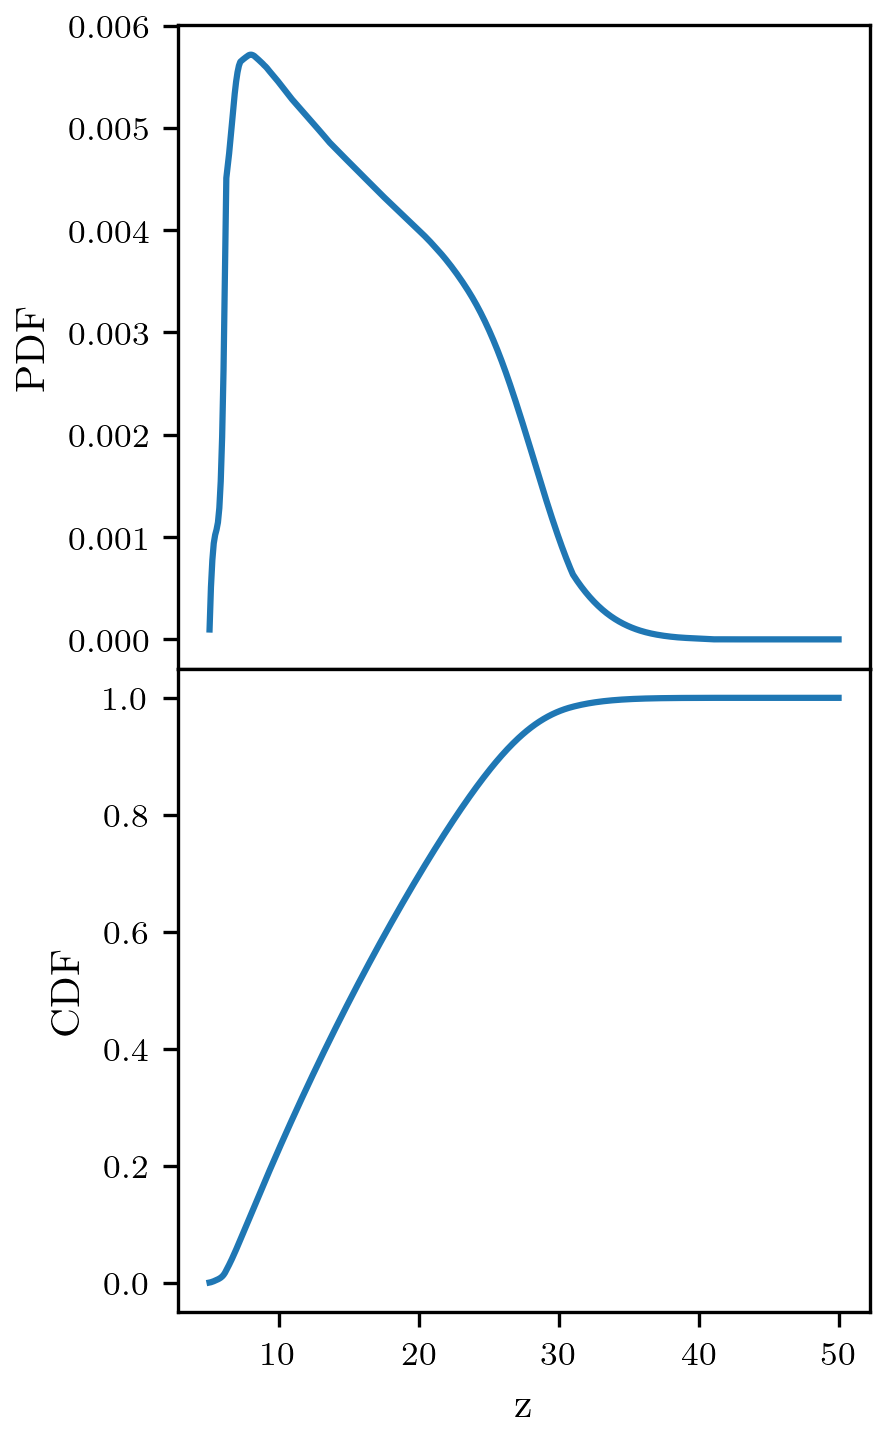
\includegraphics{globalemu/figs/cdf_and_pdf.png}
    \caption{\textbf{Top panel:} The probability distribution calculated from the difference between the maximum and minimum signal temperatures in the \cmGEM~training data set using \cref{eq:resamp-dif} and \cref{eq:resamp-prob}. \textbf{Bottom panel:} The corresponding cumulative distribution function~(CDF). We use this CDF to resample the 21-cm signals
    to better capture the variation at low redshifts and allow the emulator to more easily learn the structure of the signal.}
    \label{fig:PDF_CDF}
\end{figure}

\subsection{Output and Input Normalisation}

Neural networks typically perform better when the outputs and inputs are of order unity and uniformly distributed. Hence, it is typical to manipulate the data sets via logarithms, normalisation and/or standardisation to improve performance.

After subtracting the AFB and resampling our signals, we also proceed to divide the signals by the standard deviation across the training data set. This type of scaling was motivated by the typically used standardisation technique, however we wanted to ensure that when scaling our signals the physically significant value of $T_{21} = 0$ remained as 0.%~(an equivalence between the spin temperature and radio background, $T_s = T_r$). 
The signals shown in \cref{fig:example_signals}, as seen by the neural network, after pre-processing, are shown in \cref{fig:ppSignals}. 

For the input redshift distribution, we transform our resampled redshifts back onto a uniform distribution between 0 and 1 using the Cumulative Density Function~(CDF) detailed in the previous section. It is the combination of resampling and uniform redshift input that ensures the neural network `sees' `stretched' signals as in the left panel of \cref{fig:ppSignals}. This technique allows the neural network to interpolate the signal at redshifts it hasn't been trained on to a higher degree of accuracy, where the signals vary greatly than if we had used uniform sampling.

\begin{figure}
    \centering
    \begin{subfigure}{0.5\textwidth}
        
    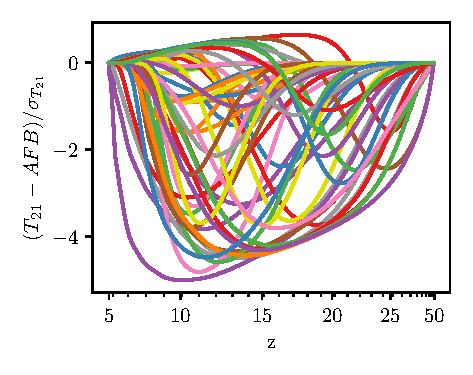
\includegraphics{globalemu/figs/preprocessed_signals.pdf}
    \end{subfigure}%
    \begin{subfigure}{0.5\textwidth}
    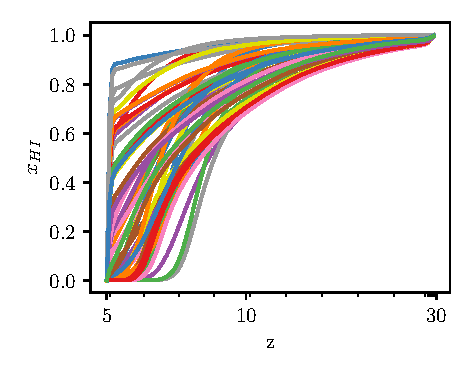
\includegraphics{globalemu/figs/xHI_preprocessed_signals.pdf}
    \end{subfigure}
    \caption{\textbf{Left Panel:} The equivalent signals from \cref{fig:example_signals} after pre-processing. Subtraction of the AFB and the subsequent resampling mean that the important information encoding the dependence on the astrophysical parameters is retained and appropriately emphasized in the training data. Here we have plotted the resampled redshift data points as being uniformly distributed, since this is how the network is set up to interpret the input. The following division by the standard deviation across the training data set scales the signals to order unity without changing the physically significant value of $T_{21}(z)=0$ where the spin temperature of the neutral hydrogen is equivalent to the radio background temperature. Minor ticks are at intervals of one on the x-axis. \textbf{Right Panel:} The equivalent neutral fraction histories from \cref{fig:example_signals} after pre-processing. For the neutral fraction histories, since the signals are already of order unity and subtraction of the equivalent AFB would not be beneficial, the pre-processing just involves resampling of the signals around regions of high variation. As with the left panel, the minor ticks are at intervals of one on the x-axis.}
    \label{fig:ppSignals}
\end{figure}

For the other input astrophysical parameters we use a Min-Max normalisation scaling each feature between 0 and 1. For example, considering the distribution of the CMB optical depth, $\boldsymbol{\tau}$ in our training data as a vector we normalise it such that
\begin{equation}
    \boldsymbol{\tilde{\tau}} = \frac{\boldsymbol{\tau} - \boldsymbol{\tau}_\mathrm{min}}{\boldsymbol{\tau}_\mathrm{max} - \boldsymbol{\tau}_\mathrm{min}}.
\end{equation}
The decision to use this type of normalisation was arrived at after testing standardisation, Min-Max normalisation and division by the max values for the input parameters while maintaining the physically motivated pre-processing for the signal temperatures detailed above. 

For $f_X$, $f_*$ and $V_c$ the distributions are uniform in log-space, and so we perform the Min-Max normalisation on the logarithm of these variables and use these as our inputs.

\subsection{$x_{HI}$ Pre-processing}
\label{neutral frac pp}

As discussed, we provide provision to emulate the neutral fraction of hydrogen as a function of redshift with \name. The pre-processing just involves resampling of the signals since:
\begin{itemize}
    \item The equivalent AFB for the neutral fraction has a value of 1 at all redshifts, and to subtract this from our training data set would just invert our signals, providing no benefit to training.
    \item The neutral fraction has a value between 0 and 1 by definition, and so we do not need to normalise the output of the network to be of order unity.
\end{itemize}

Again, resampling the signals allows the network to learn the variation in the training models and interpolation across redshift with a higher degree of accuracy. We perform the resampling with the equivalent of \cref{eq:resamp-dif} and \cref{eq:resamp-prob}. The right panel of \cref{fig:ppSignals} shows the same set of neutral fraction histories as in \cref{fig:example_signals} after pre-processing.

\section{Neural Network Structure}
\label{structure}

As stated, the goal with \name~is to maintain a simple network that is highly accurate without having to rely on non-trivial machine learning tools such as dropout, regularisation and batch normalisation. However, in the design of any neural network the optimizer, the architecture, loss function, activation function and learning rate are core considerations. 

\subsection{Architecture}

Dropout \citep{Srivastava2014} and the commonly used L1 and L2 regularisation are typically employed to prevent overfitting where the network learns the training data to such a high degree of accuracy that it is unable to generalise. Overfitting is generally a result of using a neural network that is too big and has an excessive number of layers and nodes. On the other hand, a network that is too small often produces poor quality predictions and consequently the aim is to produce a `reasonably' sized network. The scope of what constitutes a reasonably sized network is dependent on the number of input/output nodes, the variation in the training data and the complexity of the relationship between the inputs and outputs.

By using the novel approach of having redshift as an input to the network both our global signal and neutral fraction emulators have, in the case of the \cmGEM~data, eight input nodes and one output node meaning that our network can remain small. Additionally, we have made a significant effort to simplify the problem with physically motivated pre-processing, which helps to reduce what constitutes as `reasonable' size for our networks.

\name~is set up in such a way that the number of layers and layer sizes can be adjusted by the user. As a result, we do not provide a prescription of what constitutes a `reasonable' size, as this may not be pragmatic. We note, however, that a significant effort can be undertaken to determine the optimum `reasonable' architecture that maximises accuracy and that this can also be impractical. Instead, we suggest that as a minimum requirement a `reasonable' architecture for a trained \name~model should meet the following criteria:
\begin{itemize}
    \item The network should not over fit the training data otherwise the predictive power will be lost.
    \item The network should have an average accuracy that is $\lesssim 10$~\% of the expected noise of a typical global 21-cm experiment (see \cref{accuracy} for a further discussion).
\end{itemize}

Based on the above criteria, the size of our input and output layers and a minimal exploration starting from a small network, trained with the pre-processed signals, and increasing the size until our accuracy criteria was met without overfitting (see Appendix B in \cite{Bevins_globalemu_2021}) we use a network with 3 hidden layers all with 16 nodes for both the global signal and neutral fraction emulation in this chapter.

\Cref{fig:architecture} illustrates the processes used to determine our architecture for the global network. We consider a set of different network sizes with one to four layers and 4, 8, 16, 32 or 64 nodes in each layer. For each of the tested networks we run a `full' training of \name~corresponding to 12 hours on a HPC equating to approximately 250 epochs using the full \cmGEM~training data. We then assess the accuracy of the trained models using the $\approx1,700$ testing models in the \cmGEM~dataset. We compare the mean and 95 percentile $RMSE$ (see \cref{accuracy}) for each architecture. We find that a network of size [16, 16, 16] is the first to meet our target accuracy of on average 10~\% the expected noise in a global 21-cm experiment. 

While we may be able to achieve a better accuracy with a larger network this pragmatic approach leads to a sufficiently accurate network for physical signal modelling in the data analysis pipeline of a global experiment like REACH. We also note that a smaller network can be evaluated faster than a larger architecture and that this is important when we are making multiple evaluations inside a Nested Sampling loop.

\begin{figure}
    \centering
    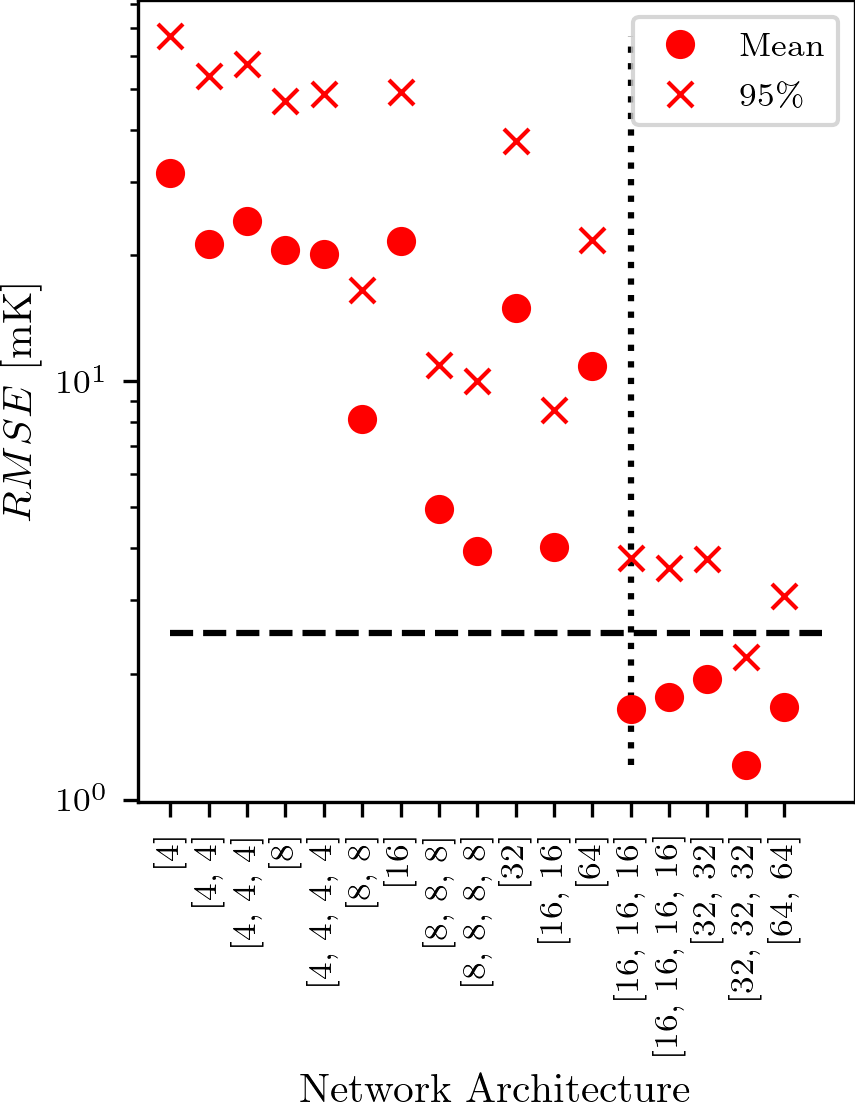
\includegraphics{globalemu/figs/Architecture.png}
    \caption{The mean and 95 percentile $RMSE$ (see \cref{accuracy}) for a set of different network architectures trained for 12h (approximately 250 epochs) on a HPC with the \cmGEM~global signal training data and assessed with the corresponding test data. The architectures have between 1 and 4 layers of varying sizes between 4 and 64 nodes. They are ordered based on the number of weights in the network (equivalent to the number of connections) as this is a useful measure of network size and an indication of predictive power. The graph is used to determine a `reasonable' architecture considering the practical target accuracy of on average 10~\% the expected noise of a global 21-cm experiment (here illustrated by the black dashed line at 2.5~mK). Throughout the rest of the chapter we use a network with 3 layers each consisting of 16 nodes which is the first to produce a mean value within our target accuracy. Our choice is highlighted with a dotted vertical line.}
    \label{fig:architecture}
\end{figure}

\subsection{Loss Function and Learning rate}

\name~uses the Mean Squared Error, typical for a regression network, as the loss function. In the case of the global signal network is given by
\begin{equation}
    MSE = \frac{1}{N} \sum_{i=0}^N (T_\mathrm{21, sim, i}(z_i) - T_\mathrm{21, pred, i}(z_i))^2
\end{equation}
where $N$ is a batch size equivalent to the number of redshift data points in each signal. $T_\mathrm{21, sim}(z)$ is the simulated signal temperature at a given redshift and $T_\mathrm{21, pred}(z)$ is the emulated equivalent. \name~trains the neural networks in batches primarily to prevent memory related issues since the training data can be large~($\approx 27,000$ models times $451$ redshift points $\approx 12$ million data points for the \cmGEM~data). We find that a reasonable batch size is equal to the number of redshift data points in each model.

For the \cmGEM~data and the \name~framework, we determine an effective learning rate to be 0.001. As with the architecture, the learning rate can be adjusted by the user of \name~to meet the requirements of the data that they are training on.

\subsection{Optimizer}

The neural network optimizer is used to change the networks hyperparameters to minimise the loss function. There are a number of different optimizers available~\citep{Ruder2016} and the choice can be dependent on the complexity of the problem and loss surface. A more robust optimizer is less likely to fall into and get stuck in local minima when training the network, resulting in more accurate emulation. Therefore, the choice of optimizer is important in designing an effective emulator. However, since \name~is designed to minimise the complexity of the relationship between the inputs and outputs and a Mean Squared Error~(MSE) loss surface is relatively smooth\footnote{This can be assessed with a plot of the loss vs epoch number during training. We find that for the results presented in \cref{sec:globalemu_results} the surface is smooth up until the loss has plateaued and training is complete, at which point we see noise like behaviour.} our choice is less consequential. We use, therefore, the commonly applied Adam~\citep{Kingma2014} optimizer which is a momentum based modified stochastic gradient descent algorithm. 

\subsection{Activation Functions}

For both the global signal and neutral fraction history network, we use a \textit{tanh} activation function in the hidden layers, which can range between (-1, 1). However, for our final layer in the global signal network we use a linear activation since the pre-processed temperature can be positive or negative and range between approximately $-4$ and $0.5$. Similar consideration is given to the output layer in the neutral fraction network, where we use a \textit{ReLU}~(Rectified Linear Unit) activation, which ensures that the output is always positive. Again, the activation functions can be changed by the user of \name~to meet the requirements of their data. We note that the above output layer activations are designed to prevent unphysical outputs, and that this is a crucial consideration for any user.

\section{Results}
\label{sec:globalemu_results}

\subsection{Emulation Time}
\label{timing}

In \cite{Cohen2020} the reported average time taken per signal with \cmGEM~is 160~ms when emulating a set of signals in a vectorised call. Here we compare the speed of \cmGEM~and \name~by emulating the 1,703 test models and taking an average time per signal. The tests are performed with \textsc{matlab} and \textsc{python} respectively on the same computer with the following processors: Intel® Core™ i3-10110U CPU @ 2.10GHz × 4. For \cmGEM~we make a vectorised call to the emulator as this results in a quicker performance then repeated single calls. We use a for loop to repeatedly call \name~which currently doesn't support such vectorised calls as they are not needed for physical signal modelling in a Nested Sampling loop\footnote{Since this work was originally published the ability to perform vectorised calls has been added to \name.}.

For \name~we record a total time of 2.29 s and a corresponding average time per signal of $1.3 \pm 0.01$ ms. In comparison, when emulating the same signals in a vectorised call with \cmGEM~we record a total time of 227.18 s and an average time per signal of 133~ms. We therefore achieve a factor of 102 improvement in emulation time with \name. We note that when using the \textsc{pymatbridge} (\url{https://github.com/arokem/python-matlab-bridge}) \textsc{python} wrapper for \textsc{matlab} the average time take to run a single prediction with \cmGEM~using a vectorised call is comparable to a direct call in \textsc{matlab}.

\subsection{Measuring Accuracy}
\label{accuracy}
In this section we primarily consider the accuracy of the global signal emulator. We note, as previously stated, that the relationship between the neutral fraction and the astrophysical parameters is expected to be simpler and therefore easier to learn.

To assess the accuracy of \name~when emulating a global 21-cm signal simulation we use a combination of two metrics; the root mean squared error~($RMSE$) and the normalised $RMSE$ given in \cite{Cohen2020} as
\begin{equation}
    \widetilde{RMSE} = \frac{RMSE}{max|T_\mathrm{21, sim}(z)|},
    \label{eq:gemloss}
\end{equation}
where
\begin{equation}
    RMSE = \sqrt{\frac{1}{N} \sum_{i=0}^N(T_\mathrm{21, sim, i}(z_i) - T_\mathrm{21, pred,i}(z_i))^2}.
\end{equation}
For the neutral fraction network $\widetilde{RMSE}$ and the ${RMSE}$ are equal since $max|x^{HI}_\mathrm{sim}(z)| = 1$. We assess the accuracy in the uniform redshift space, and consequently our assessment is independent of the loss function used for training.

$\widetilde{RMSE}$ is a dimensionless quantity used by \cmGEM~and by assessing the quality of our network with this metric we can make direct comparisons between the two emulators. We also want our emulator to have an accuracy significantly lower than the expected noise of a global 21-cm experiment. This is required if the emulator is to be used to confidently model the 21-cm signal and draw conclusions about the astrophysics during the CD and EoR. To assess this accuracy requirement, we can use the dimensionful $RMSE$ metric. 

As highlighted in the previous section, we suggest an average accuracy of $\lesssim 10$~\% the expected noise of a global 21-cm experiment such as REACH, equivalent to an $RMSE\lesssim 2.5$~mK, to be a sufficient limit. Since the accuracy of emulation is a function of the bandwidth, we report the accuracy across the entire range of the simulations $z = 5-50$~($z=5-30$ for the neutral fraction network) and across the expected REACH Phase I bandwidth of $z = 7 - 28$ \cite{de_lera_acedo_reach_2022}. %It is also a practical target, 
The noise in a 21-cm experiment has a fundamental effect on our confidence in any astrophysical parameter values inferred from the data, and, given our target accuracy, this will likely be larger than the uncertainty introduced from \name.

\subsection{Global 21-cm Signal}

\cref{fig:bestWorst} shows that the mean $RMSE$ value across the redshift range $z=5 - 50$ is 1.85 mK and that the maximum value is 10.26 mK. Further, \cref{tab:full_results} shows that performing the same calculation of the $RMSE$ inside the REACH band, $z=7-28$ gives a mean value of $2.52$ mK which is very close to the desired $2.5$~mK limit. We also report in the table the $RMSE$ value for which $95$~\% of the models have a value smaller than or equal to. In the REACH band, this equates to $5.37$ mK. For all the reported results, the 95 percentile is significantly lower than the maximum values (a factor of 3 for the global signal and a factor of approximately 1.5 to 2 depending on bandwidth for the neutral fraction). This means that out of a set of $1,703$ global signals only 85 have $RMSE$ values above $3.90$ mK across the band $z = 5-50$ for example. We note that the values reported, averages across redshift ranges, in the REACH band are generally higher than across the whole redshift range because the REACH band excludes redshifts $\gtrsim 30$ where the emulation is expected to be very precise.

Appendix C in \cite{Bevins_globalemu_2021} shows the error as a function of the explored parameter space for the global 21-cm signal in the \cmGEM~test data set.

In \cref{tab:full_results}, we also report the $\widetilde{RMSE}$ values in both the REACH band and across the whole redshift range. \cite{Cohen2020} report similar results for \cmGEM. When training and testing on the same data sets, we recover a mean $\widetilde{RMSE}$ of 1.12~\% compared to 1.59~\% when using \cmGEM. Similarly, we report a maximum value of $6.32$~\% in comparison to the value of $10.55$~\% reported for \cmGEM. \name~can achieve a high degree of accuracy in its emulation.

\begin{figure}
    \centering
    \begin{subfigure}{0.5\textwidth}
        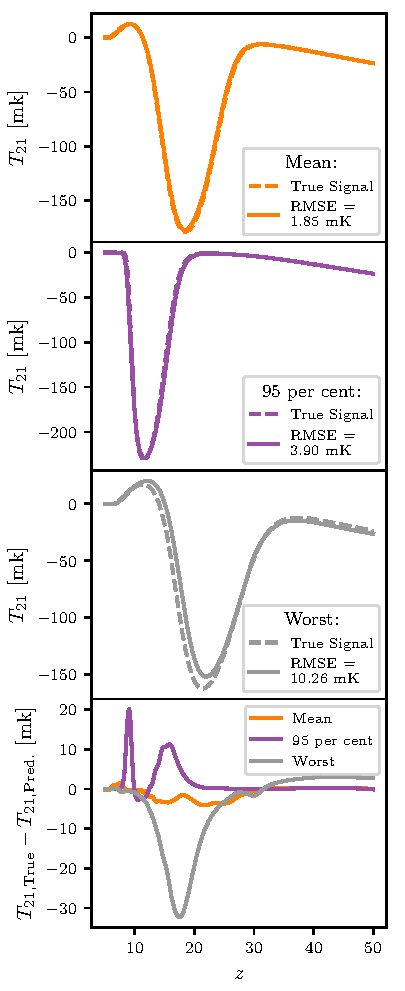
\includegraphics{globalemu/figs/test_best_worst_T.pdf}
    \end{subfigure}%
    \begin{subfigure}{0.5\textwidth}
        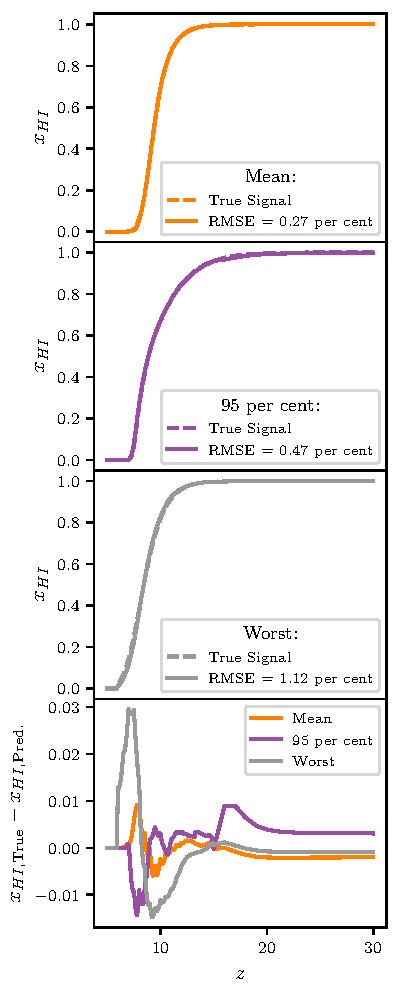
\includegraphics{globalemu/figs/test_best_worst_xHI.pdf}
    \end{subfigure}
    \caption{\textbf{Left Panel:} The top three panels show the mean, 95 percentile and the worst emulations respectively, based on the $RMSE$, for the global 21-cm signal across the entire test set of 1,703 models. The bottom panel shows the difference between the simulations and predictions as a function of redshift. Full details of the accuracy of the emulation can be found in \cref{tab:full_results}, and a discussion can be found in the text. \textbf{Right Panel:} The top three panels show the mean, 95 percentile and the worst emulations respectively for the neutral fraction history across the entire test set of 791 models and the difference between the simulations and predictions is shown in the bottom panel. The level of accuracy here is higher than that for the global signal, despite using a similar pre-processing and identical network, demonstrating that the relationship between the astrophysical parameters, redshift and the network output is simpler here.}
    \label{fig:bestWorst}
\end{figure}

\subsection{Neutral Fraction}

For the neutral fraction history network, we show similar results. The right panel of \cref{fig:bestWorst} demonstrates the quality of the emulation with the mean, 95 percentile and the worst results when emulating the neutral fraction and these values are detailed in \cref{tab:full_results}. The results generally are of higher quality than that for the global signal and, noting that the pre-processing for the two networks is near identical and the networks themselves are of the same size, this supports the understanding that the relationship between the inputs and outputs is simpler here. In the band $z = 5 -30$ only 39 of 791 test models have $\widetilde{RMSE} \geq 0.47$~\%.

\begin{table*}
    \centering
    \begin{tabular}{|c|c|c|c|c|c|}
        \hline
         & & \multicolumn{2}{|c|}{Global Signal} & \multicolumn{2}{|c|}{Neutral Fraction} \\
         \hline
         & & $z = 5- 50$& $z = 7- 28$& $z = 5- 30$& $z = 7- 28$ \\
         \hline
         \multirow{4}{4em}{$RMSE$}& Minimum &  0.30 mK &  0.31 mK& 0.09~\% & 0.08~\% \\
         & Mean & 1.85 mK& 2.52 mK& 0.29~\% & 0.26~\% \\
         & $95^{th}$ percentile& 3.90 mK& 5.37 mK& 0.47~\%& 0.44~\%\\
         & Maximum & 10.26 mK& 15.10 mK& 1.12~\% & 0.65~\% \\
         \hline
         \multirow{4}{4em}{$\widetilde{RMSE}$}& Minimum & 0.21~\% & 0.26~\%& -- & -- \\
         & Mean & 1.12~\% & 1.53~\% & -- & -- \\
         & $95^{th}$ percentile& 2.41~\% & 3.22~\% & -- & -- \\
         & Maximum & 6.32~\% & 9.31~\% & -- & -- \\
         \hline
    \end{tabular}
    \caption{Detailed results of the emulation using \name~and the \cmGEM~training and test data for both the global signal and the neutral fraction history. We find that \name~ achieves the desired accuracy of on average $\approx 10$~\% the expected noise of a typical global 21-cm experiment (equating to $\approx 2.5$~mK in the REACH band of $z=7-28$). Of note are the recorded $95$~\% percentiles, the $RMSE$ for which $95$~\% of the models have values smaller than or equal to, which are significantly lower than the maximum $RMSE$ values. A discussion comparing the results of \cmGEM~and \name can be found in the text. We find that our global signal emulator has a maximum $\widetilde{RMSE}$ approximately half that achieved with \cmGEM. For the neutral fraction $RMSE = \widetilde{RMSE}$. We find a higher degree of accuracy for the neutral fraction with an identical network and similar pre-processing, indicating a simpler relationship.}
    \label{tab:full_results}
\end{table*}

\section{Conclusions}
\label{sec:globalemu_conclusions}

\name~uses a novel approach to emulate, with neural networks, the global 21-cm signal and the evolution of the neutral fraction during the CD and EoR by considering redshift as an input to the neural networks alongside the astrophysical parameters. In tandem with this reparameterisation of the problem, we use a predominantly physically motivated pre-processing for both the global signal and neutral fraction. We subtract from the global signals an astrophysics free baseline, which obviates the need for the network to learn a non-trivial but well-understood relationship at high redshift. We then resample both the global signals and neutral fractions so that the regions which vary significantly across the training data sets can be better characterised by the networks.

The above framework allows the complex relationships between the astrophysical parameters and the global signal or neutral fraction history as functions of redshift to be effectively learnt with small neural networks. Each high resolution global signal of 451 redshift data points can be emulated in on average $1.3$~ms. We note that this is a factor of approximately $102$ improvement on the 133~ms we record with \textsc{matlab} when predicting the same signals on the same computer with \cmGEM.

We demonstrate the effectiveness of \name~by using the \cmGEM~training and testing data. This allows for a direct comparison between our results and the results of \cmGEM. We find that \name~can emulate to a higher degree of accuracy the global 21-cm signal than \cmGEM~with a maximum normalised $RMSE$ of 6.32~\% in comparison to 10.55~\% over the range $z = 5 -50$. We also demonstrate that \name~can emulate a global 21-cm signal to, on average, less than 10~\% the expected noise of a global 21-cm experiment like REACH.

Finally, \name~is a flexible \textsc{python} package that can be easily retrained on updated models with new astrophysical dependencies. For example, additional astrophysical phenomena such as Lyman-$\alpha$ heating \citep{Reis_sta_2021} or additional radio background produced by galaxies (or an indeterminate synchrotron-like source) \citep{Fialkov2019, Reis2020} can be incorporated and easily trained upon, as shown in the second half of this thesis. While the results achieved with the \cmGEM~data are impressive, the novelty of \name~is in its flexibility, incorporation of redshift as an input and physically motivated pre-processing. Particularly the final two points allow for an accurate mapping from parameters to temperature with a single neural network reducing the points of failure and need for excessive fine-tuning.

\name~has been used to emulate models from the ARES\cite{ARES_sim} simulation code by members of the Network for Exploration and Space Science research group at the University of Colorado Boulder. Further, \name~influenced the design of the power spectrum emulator used in the recent HERA analysis (section 7.5 \cite{HERA_2022c}).

\begin{comment}
\renewcommand\thesection{\arabic{chapter}.\Alph{section}}

\section{Calculating the Astrophysics Free Baseline}
\label{appendixA}

To approximate the astrophysics free baseline~(AFB) we need to consider the physics defining the signal structure during the period dominated by collision coupling. During this period neutral hydrogen atoms collide with other neutral hydrogen atoms, protons and electrons. The spin temperature of hydrogen is coupled to the gas temperature, $T_K$, via the collisions and that temperature cools adiabatically at a faster rate than the background radiation, $T_r$. The spin temperature, $T_s$, which encodes the number of hydrogen atoms in the two hyperfine levels of the ground state \citep{Furlanetto_review_2006} during this period is given by
\begin{equation}
    \frac{1}{T_s} = \frac{1/T_r + x_c/T_K}{1+x_c}
\end{equation}
where $x_c$ is the collisional coupling coefficient. For our approximation of the AFB calculated here we use a reference value for the gas temperature of $T_{K\mathrm{, ref}} = 33.7340$~K at $z_\mathrm{ref} = 40$ from the simulations used to produce the training and test data sets. We then scale $T_{K\mathrm{, ref}}$ adiabatically using
\begin{equation}
    T_K = T_{K\mathrm{, ref}} \frac{(1 + z)^2}{(1+z_\mathrm{ref})^2}
\end{equation}
to get $T_K$ as a function of redshift.

The coupling is dominated by H-H collisions and so we only consider these in our simulation. The coupling coefficient for this interaction is given by \cite{Furlanetto_review_2006}
\begin{equation}
    x_c^{HH} = \frac{n_H \kappa_{10}^{HH} T_*}{A_{10} T_r},
\end{equation}
where $\kappa_{10}^{HH}$ is the rate coefficient for the spin deactivation of neutral hydrogen, $T_*$ is the energy defect and $A_{10}$ is the spontaneous emission coefficient of the 21-cm transition. $n_{H}$ is the relative number density of neutral hydrogen given by as
\begin{equation}
    n_H = 3.40368\times 10^{68}~\frac{\rho_c}{m_p} (1 - Y) \Omega_b (1 + z)^3
\end{equation}
where $Y=0.274$ and is the Helium abundance by mass, $\rho_c$ is critical mass density of the universe in $M_\mathrm{sol}/$cMpc$^3$, $m_p$ is the proton mass in $M_\mathrm{sol}$ and $\Omega_b$ the the baryon density parameter.

From the above we can then calculate $\delta T$ as
\begin{equation}
    \delta T = \frac{T_s - T_r}{1 + z}(1 - \exp(-\tau_{\nu_0})),
\end{equation}
where $\tau_{\nu_0}$ is the 21-cm optical depth of the diffuse IGM
\begin{equation}
    \tau_{\nu_0} = \frac{3 h c^3 A_{10} x_{HI} n_H}{32 \pi k_b T_s \nu_0^2 H(z)},
\end{equation}
where $\nu_0$ is the rest frequency of the 21-cm emission and $H(z)$ is the Hubble rate. In our calculation we use the same cosmological parameters that were used to generate the signals \citep[see][]{Cohen2020}. Here the neutral fraction, $x_{HI}$ has a value of 1 since there is no astrophysics involved in the AFB.

\section{Testing the neural networks for overfitting}
\label{app:overfitting}

We can demonstrate that, for both the global signal and neutral fraction, the chosen network sizes of 3 hidden layers of 16 nodes do not overfit the training data by comparing the distribution of loss values across the training and test data sets. This is shown in \cref{fig:globalsignaloverfitting} and \cref{fig:xhioverfitting} for the global signal and neutral fraction respectively. Again, we have used a gaussian kernal density estimation to calculate continuous probability density curves from the discrete histograms of losses. We can see in both cases that the loss, evaluated with \cref{eq:gemloss}, for the testing and training data sets, when emulated with the trained neural networks, have similar distributions and can consequently conclude that the neural networks are not overfitting the training data. In the event that the training data was being overfit then the purple distribution, showing the training data losses, would peak to the left of the orange distribution, showing the test data losses, because the network would have learnt the training data to such a high degree of accuracy that it cannot generalise well to the testing data.

\begin{figure}
    \centering
    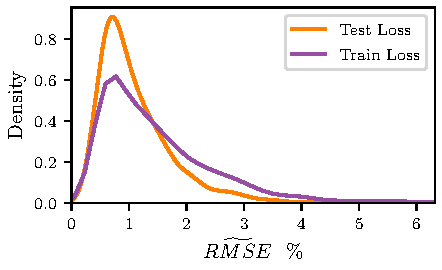
\includegraphics{globalemu/figs/GlobalSignalOverfittingCheck_GEMLossKDE.pdf}
    \caption{The probability density for the loss distribution found when emulating the training and test data sets for the global 21-cm signal with \name.}
    \label{fig:globalsignaloverfitting}
\end{figure}

\begin{figure}
    \centering
    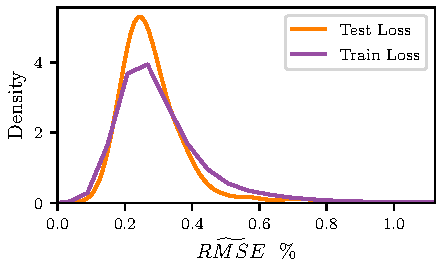
\includegraphics{globalemu/figs/xHIOverfittingCheckKDE.pdf}
    \caption{The probability density for the loss distribution found when emulating the training and test data sets for the neutral fraction with \name.}
    \label{fig:xhioverfitting}
\end{figure}

\section{Error Vs Parameter}
\label{paramVsError}

\Cref{fig:paramVsError} shows the parameter space explored in the \cmGEM~test data set as a scatter plot. The data points are coloured based on the $RMSE$ value calculated when comparing the corresponding true signal with the emulation, over the range $z = 5 - 50$, from \name. 

\Cref{fig:paramVsErrorGEM} shows the equivalent graph with the colours determined using the dimensionless $\widetilde{RMSE}$ metric across the band $z = 5 - 50$.

\begin{figure*}
    \centering
    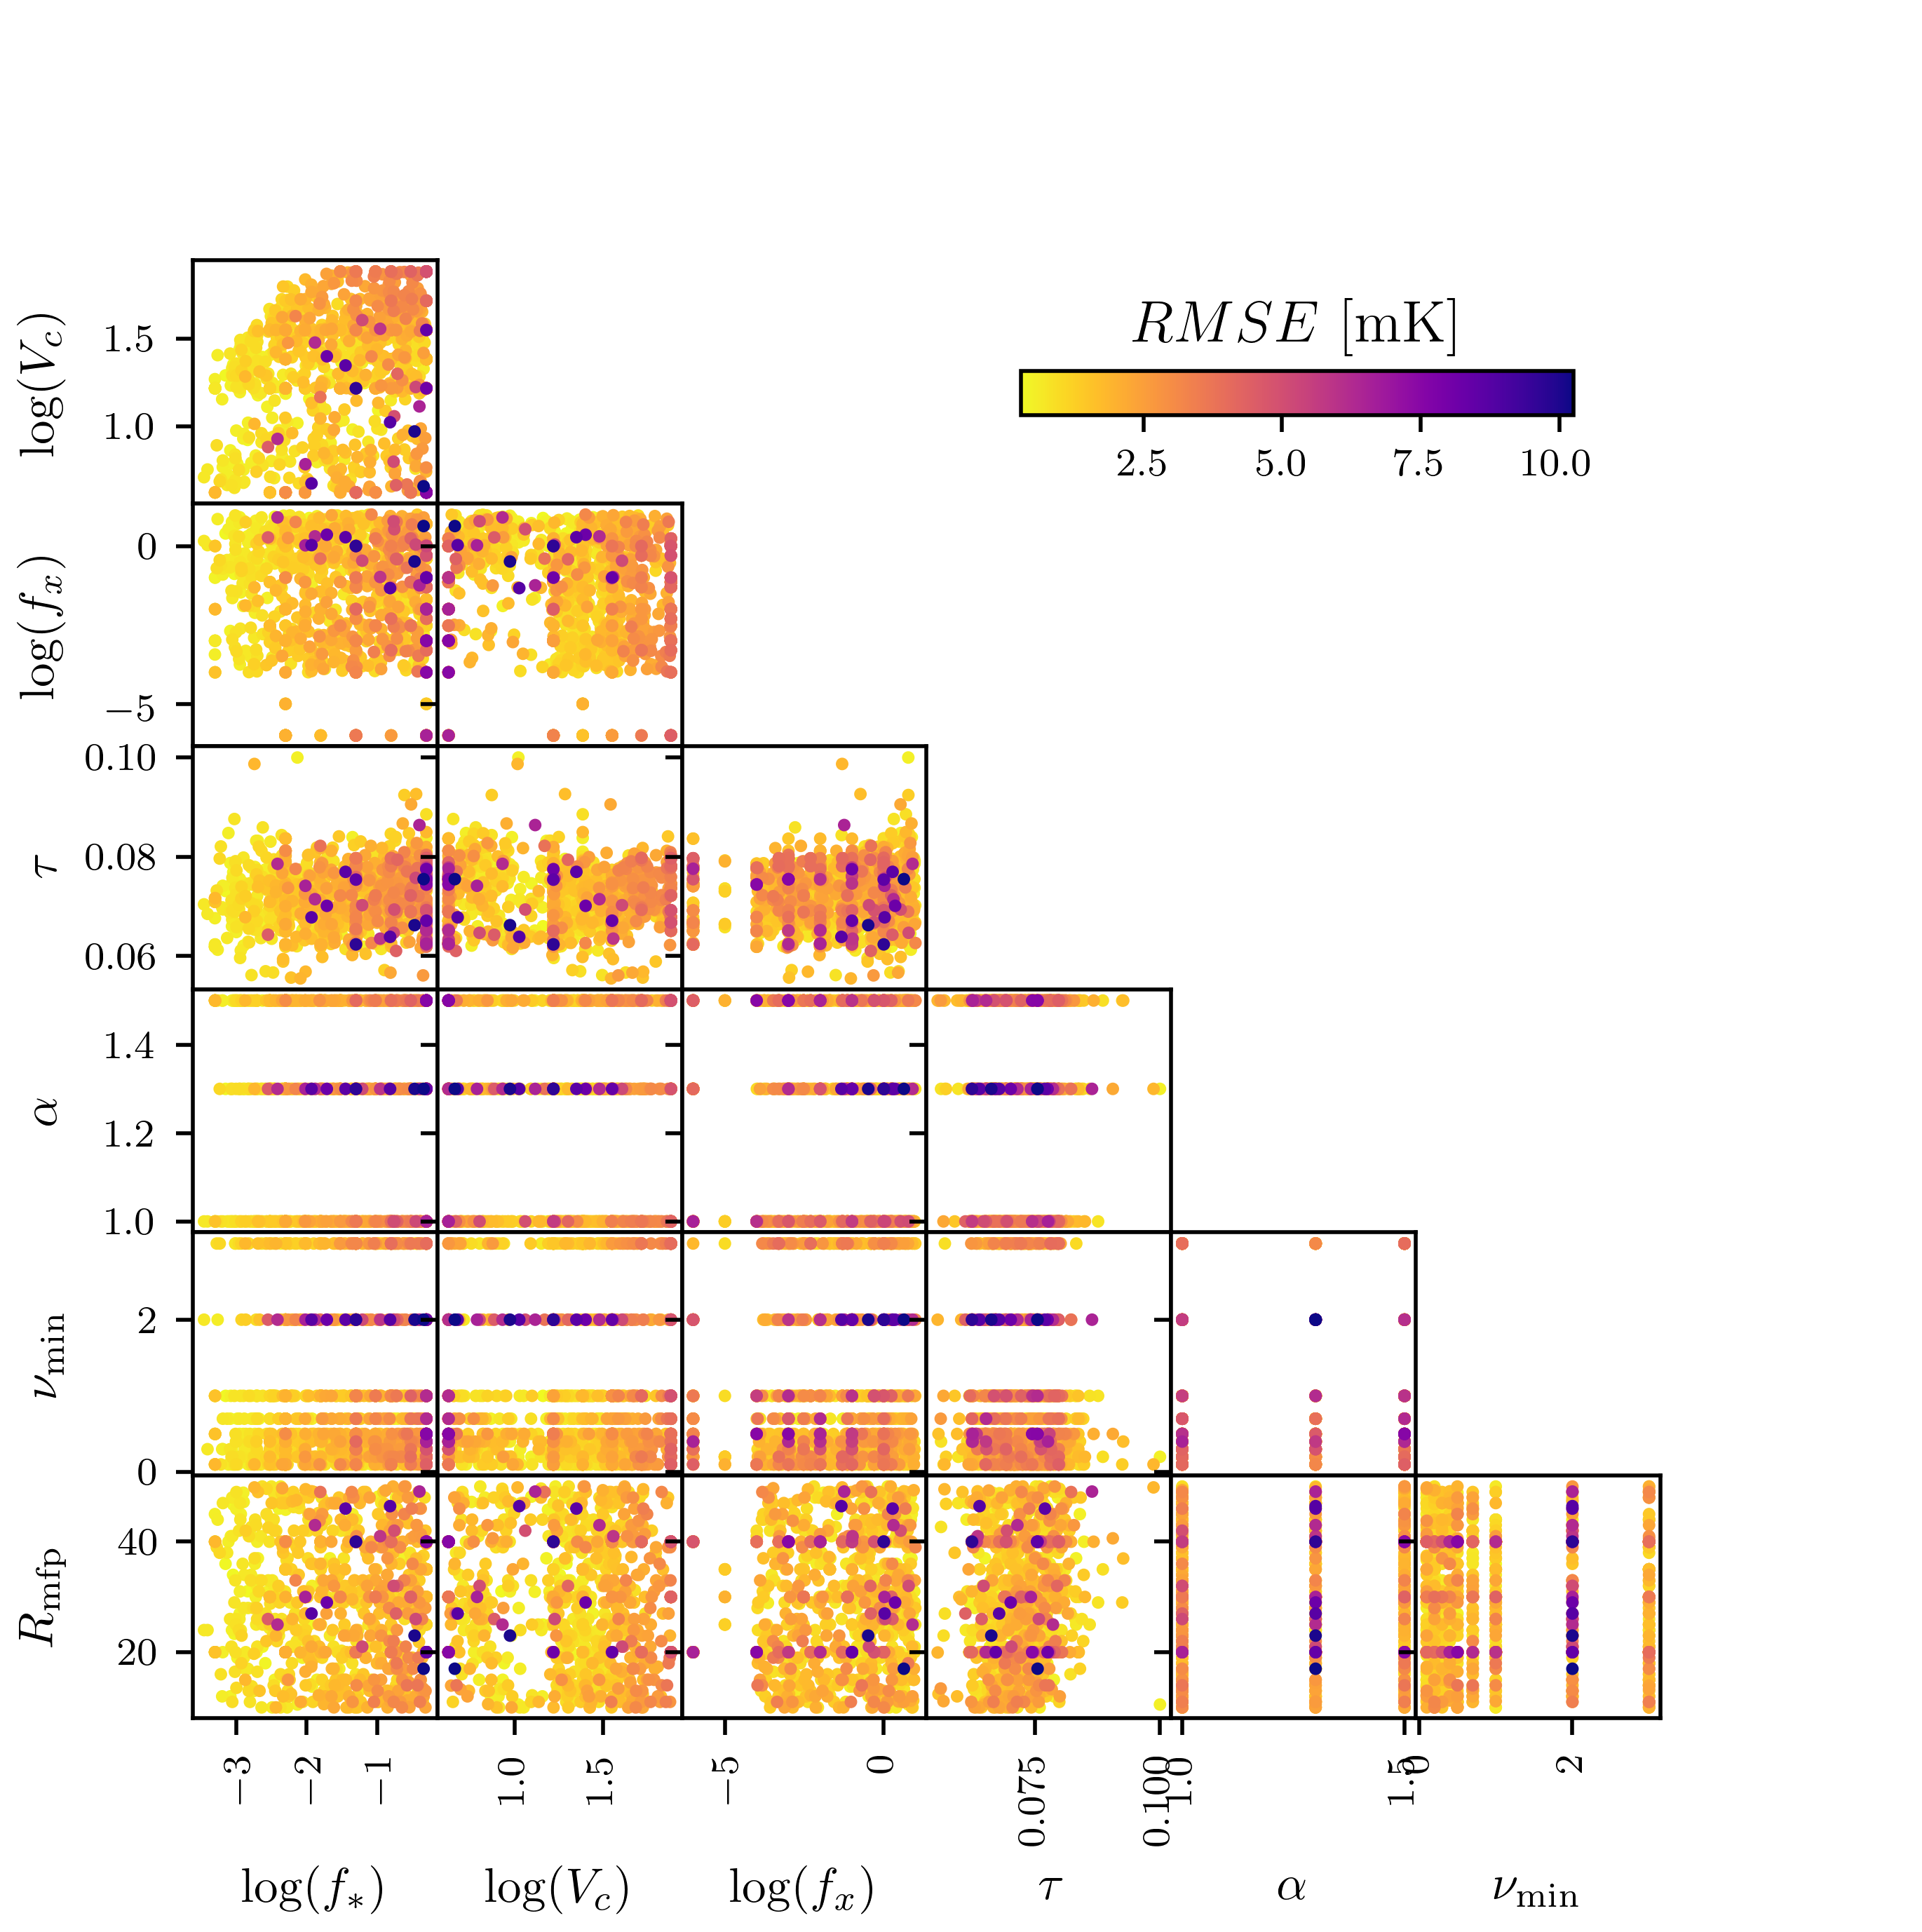
\includegraphics{globalemu/figs/ParamsVsError.png}
    \caption{The parameter space explored by the \cmGEM~test data set. Each panel shows the $1,703$ models plotted as data points based on the corresponding astrophysical parameter values. They are coloured according to the $RMSE$ calculated when comparing the true signals to the emulation from \name~across the range $z = 5-50$.}
    \label{fig:paramVsError}
\end{figure*}

\begin{figure*}
    \centering
    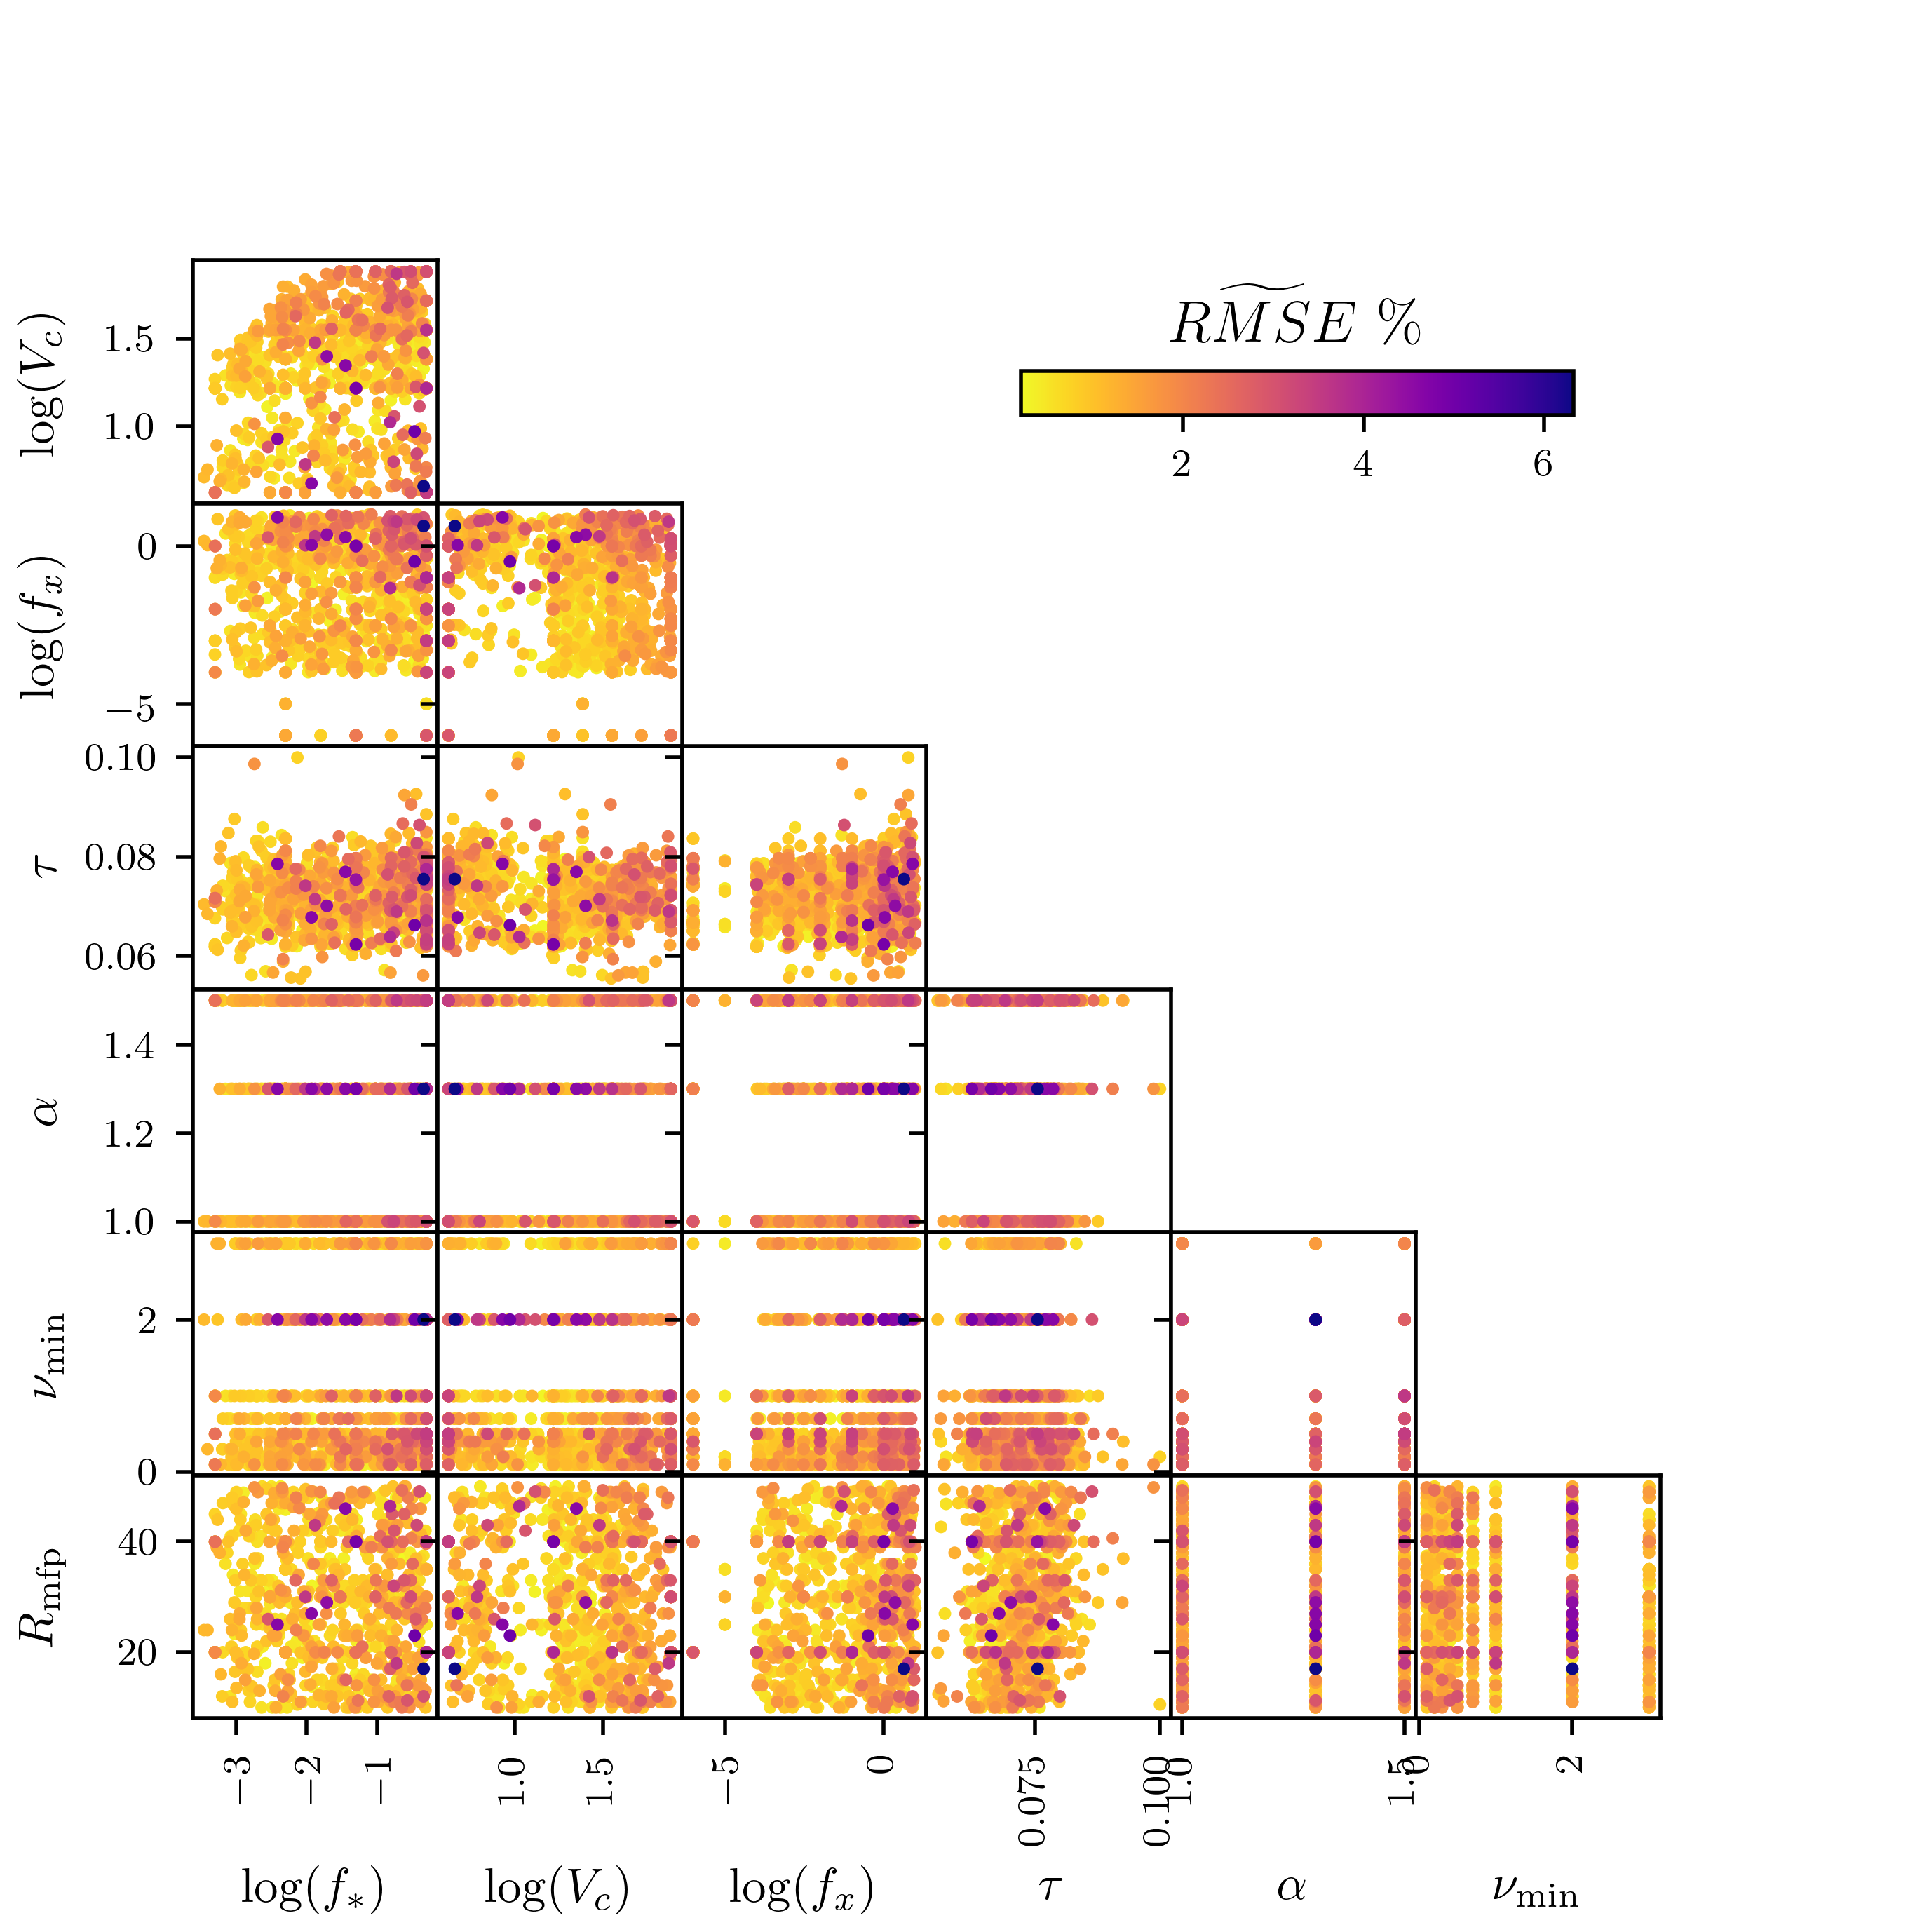
\includegraphics{globalemu/figs/ParamsVsError_GEM.png}
    \caption{The equivalent of \cref{fig:paramVsError} with the data points colored based on the dimensionless $\widetilde{RMSE}$ error calculated across the band $z = 5 - 50$.}
    \label{fig:paramVsErrorGEM}
\end{figure*}

\end{comment}

\chapter{\textsc{margarine}}
\label{ch:margarine}
\section{Introduction}

%Bayesian analysis is a cornerstone of modern statistical inference. It uses Bayes theorem to iteratively update the probability of a given hypothesis or model (posterior) given existing knowledge about the model parameters (prior) and a representative probability distribution for the data given the choice of model and parameters at each iteration (likelihood). Various computational approaches to Bayesian analysis exist, including Markov Chain Monte Carlo~(MCMC) methods \citep[e.g.][]{emcee} and Nested Sampling algorithms \citep[e.g.][]{polychord_2015, polychord_2015b}.

Bayesian analysis has been applied in the inference of cosmological parameters from experiments such as the CMB mapper Planck~\cite{Planck2018}, the Dark Energy Survey~(DES, \citep{DES_Year1_2018, DES_year3_2021, DES_year3}), 21-cm power spectrum experiments~(such as HERA~\citep{HERA_2022b}, LOFAR~\citep{Ghara_LOFAR_2020, Mondal_LOFAR_2020} and MWA~\citep{Greig_MWA_2020, Ghara_MWA_2021}) and global or sky-averaged 21-cm experiments such as
REACH~\citep{Anstey_REACH_2021} and SARAS \citep{Bevins_SARAS2_2022, Bevins_saras3_2022}. 

These experiments are often plagued by `nuisance' parameters that characterise foregrounds and instrumental effects in the data. This leads to high dimensional parameter spaces, of which only a few of the parameters model the core science. Consequently, drawing conclusions about the parameters of interest and making comparisons of different experiments can be challenging. For example, in the Year 1 analysis of data from DES the likelihood contains a total of 26 parameters of which 20 could be considered nuisance parameters with only 6 corresponding to cosmological parameters of interest~\citep{DES_Year1_2018}. Similarly, for REACH \citep{Anstey_REACH_2021, de_lera_acedo_reach_2022} the likelihood can contain around 20–30 parameters, with only 3-7 of these corresponding to the signal.

In this chapter, we present a post-processing tool called \textsc{margarine} that can be used to calculate \emph{marginal} or \emph{nuisance-free} posterior distributions pertaining to the core science goals of the above experiments through density estimation with Masked Autoregressive Flows~(MAFs, \cite{Papamarkarios_MAF_2017}) and Kernel Density Estimators~(KDEs, \cite{rosenblatt_KDE_1956, parzen_KDE_1962}).

Due to the ubiquity of Bayesian analysis in cosmology, post-processing of samples from MCMC and Nested Sampling algorithms is an important area of research. \textsc{margarine} is an invaluable addition to the Bayesian workflow and allows for direct and specific comparison of the constraining ability of different experimental approaches, rapid emulation of nuisance-free likelihoods and experimentally informed priors.

We implement our approach in \textsc{Python} using \textsc{tensorflow} and the \textsc{keras} backend and release the code as the pip installable package \textsc{margarine}. The code is fully documented with worked examples, subject to continuous integration testing and does not require high performance computing to be used.

In \cref{sec:motivation}, we briefly outline the motivation behind the development of \textsc{margarine}. In \cref{sec:theory}, we reintroduce Bayesian analysis and discuss the marginal statistical quantities that can be calculated with \textsc{margarine}. We discuss the two different types of density estimators used by \textsc{margarine} in \cref{sec:density_estimators}. In \cref{sec:applications}, we demonstrate several applications of the code base, including applications to samples from the Dark Energy Survey, Planck and mock observations with the REACH pipeline. We summarise the chapter in \cref{sec:conclusions_margarine}.

%\textsc{margarine} was previously introduced in the conference proceedings for the 2022 International Conference on Bayesian and Maximum Entropy Methods in Science and Engineering \citep[MaxEnt22, ][]{margarine_maxent} in which the nuisance-free likelihood was derived and demonstrated. We review this work briefly in this chapter.

\Cref{sec:marginal_likelihood} was first drafted by Will Handley for \cite{margarine_maxent}, edited by the author and visualized in \cref{fig:pipeline} and \cref{fig:pipelineB} by the author. The co-authors, Will Handley, Pablo Lemos, Peter Sims, Eloy de Lera Acedo, Anastasia Fialkov and Justin Alsing, of \cite{margarine_maxent} and \cite{margarine_neurips} provided comments on the manuscripts that this chapter is adapted from.

\section{Motivation}
\label{sec:motivation}

If our model $M (\Theta)$ contains nuisance, $\alpha$, and cosmological signal parameters, $\theta$, then we can write $\Theta = \{\alpha, \theta\}$. Mathematically, the marginal posterior for the signal parameters, $\mathcal{P}(\theta)$, can be calculated by integrating out the dependence on $\alpha$
\begin{equation}
    \mathcal{P}(\theta) = \int \mathcal{P}(\alpha, \theta) d \alpha.
    \label{eq:marginal_posterior}
\end{equation}
However, $\mathcal{P}(\theta)$ is typically a difficult quantity to calculate. We can effectively perform this marginalisation by training density estimators on samples in $\theta$ from MCMC or Nested Sampling chains. From these density estimators, we can generate samples from the marginal distribution $\mathcal{P}(\theta)$ and importantly calculate $\log \mathcal{P}(\theta)$ for a given set of $\theta$, which gives us access to a whole host of previously intractable marginal summary statistics.

For example, the marginal Kullback-Leibler~(KL) divergence tells you how much information is gained by contracting specifically the core science prior onto the core science posterior without including contributions from correlations with or constraints on the nuisance parameters. This allows us to confidently compare the information gained from different data sets from different experiments measuring the same signal, regardless of their specific instrumental nuances. Similarly, the marginal Bayesian Model Dimensionality~(BMD) can be used to compare the effective number of core science parameters constrained by different experiments and models. Both the \emph{marginal} KL divergence and the BMD, therefore, provide a way to quantitatively determine which experimental approaches are the most informative, which can inform improvements to instrumentation in the future and prior to \textsc{margarine} was not as easy to assess.

Using normalised density estimators to calculate the KL divergence, marginal or not, also has the added advantage that it does not require knowledge of the Bayesian evidence, which is not always accessible.

Further, since the density estimators can be used to empirically approximate the logarithm of any posterior distribution, then they can be used as a computationally inexpensive likelihood generator. In practice, we can take advantage of this to perform efficient analysis of constraints from multiple different experiments as demonstrated in this chapter and further in \cref{ch:hera_saras3}.

Finally, we note that if the density estimator is set up correctly such that it is a bijective transformation between the unit hyper-cube and the target posterior, then it can be used to generate the prior on a subsequent Nested Sampling run. This allows you to use far more complex priors based on current experimental results, incorporating our current knowledge of the parameter space~\citep{Alsing_bijectors_2021}.

\section{Theory}
\label{sec:theory}

\subsection{Bayesian analysis}
\label{sec:bayesian_inference}

Bayesian analysis is concerned with the estimation of posterior probabilities using Bayes theorem
\begin{equation}
    P(\Theta | D, M) = \frac{P(D| \Theta, M) P(\Theta|M)}{P(D|M)} = \frac{\mathcal{L}(\Theta)\pi(\Theta)}{\mathcal{Z}},
    \label{eq:bayes_theorem}
\end{equation}
where $\Theta$ are the parameters of our model $M$ describing the data $D$ and $\mathcal{L}(\Theta)$ corresponds to the likelihood. The likelihood is often assumed to be Gaussian in nature (although more complicated likelihoods can be implemented~\cite{Scheutwinkel2022a}). The prior, $\pi(\Theta) = P(\Theta|M)$, encodes our existing knowledge about the parameters before any sampling is performed. $\pi(\Theta)$ is often chosen to be uniform or log-uniform for each parameter, however we would often like to inform this with existing experimental results.

The evidence, $\mathcal{Z}$, is a (fully-)marginal likelihood integrated over all the parameters and weighted by the prior
\begin{equation}
    \mathcal{Z} = \int \mathcal{L}(\Theta)\pi(\Theta)d\Theta.
    \label{eq:evidence}
\end{equation}

\subsection{Nuisance-free likelihood}
\label{sec:marginal_likelihood}

We can re-write Bayes theorem as
\begin{equation}
     \mathcal{L}(\theta,\alpha)\times \pi(\theta,\alpha) =\mathcal{P}(\theta,\alpha)\times \mathcal{Z},
    \label{eqn:bayes}
\end{equation}
with the inputs of inference (likelihood and prior) on the left-hand side, and the outputs (posterior and evidence) on the right.

We may marginalise any probability distribution so can, in addition to the definition of the nuisance marginalised posterior, straightforwardly define the nuisance marginalised prior by integrating over $\alpha$
\begin{equation}
    \pi(\theta) = \int \pi(\theta,\alpha)d\alpha.
    \label{eqn:marginal}
\end{equation}
The nuisance marginalised version of Bayes theorem~\cref{eqn:bayes} takes the form
\begin{equation}
    \mathcal{L}(\theta)\times\pi(\theta) = \mathcal{P}(\theta)\times\mathcal{Z}.
    \label{eqn:marginal_bayes}
\end{equation}
Here $\mathcal{Z}$ is the original evidence, whilst $\mathcal{L}(\theta)$ is non-trivially the \emph{nuisance-free likelihood}
\begin{equation}
    \mathcal{L}(\theta) 
\equiv \frac{\int\mathcal{L}(\theta,\alpha)\pi(\theta,\alpha)d\alpha}{\int \pi(\theta,\alpha)d\alpha} = \frac{\mathcal{P}(\theta)\mathcal{Z}}{\pi(\theta)},
    \label{eqn:partial}
\end{equation}
where the above is motivated by marginalising Bayes theorem over $\alpha$, and substituting the definitions in \cref{eqn:partial,eq:marginal_posterior,eqn:marginal} recovers the marginalised Bayes theorem~\cref{eqn:marginal_bayes}.

The nuisance-free likelihood \cref{eqn:partial} is straightforward to compute in our framework since we (uniquely) have Nested Sampling-computed evidences $\mathcal{Z}$ and we can generate emulators for the distributions $\mathcal{P}(\theta)$ and $\pi(\theta)$ with \textsc{margarine}.

Let $\mathcal{L}_A(\theta,\alpha_A)$ and $\mathcal{L}_B(\theta,\alpha_B)$ be two likelihoods for distinct datasets, each with their own nuisance parameters. The nuisance-free likelihoods $\mathcal{L}_A(\theta)$, $\mathcal{L}_B(\theta)$ form a lossless compression in $\theta$. This means that we can recover the same (marginal) inference in combination that we would have made when performing a combined analysis with all nuisance parameters:
\begin{align}
    \mathcal{L}_A(\theta,\alpha_A)\mathcal{L}_B(\theta,\alpha_B)\pi_{AB}(\theta,\alpha_A,\alpha_B) &=  \mathcal{P}_{AB}(\theta,\alpha_A,\alpha_B)\mathcal{Z}_{AB},  \label{eqn:combined_bayes}\\
    \Rightarrow
        \mathcal{L}_A(\theta)\mathcal{L}_B(\theta)\pi(\theta) &=  \mathcal{P}_{AB}(\theta)\mathcal{Z}_{AB}, 
        \label{eqn:marginal_combined_bayes}
\end{align}
 if their respective priors $\pi_A(\theta,\alpha_A)$ and $\pi_B(\theta,\alpha_B)$ satisfy the marginal consistency relations:
\begin{gather}
    \pi(\theta) = \int \pi_A(\theta,\alpha_A)d\alpha_A = \int \pi_B(\theta,\alpha_B)d\alpha_B,  
    \label{eqn:marginal_A}\\
    \int \pi_{AB}(\theta,\alpha_A,\alpha_B)d\alpha_A = \pi_B(\theta,\alpha_B), \qquad \int \pi_{AB}(\theta,\alpha_A,\alpha_B)d\alpha_B = \pi_A(\theta,\alpha_A).
    \label{eqn:marginal_B}
\end{gather}
This process is represented graphically in \cref{fig:pipeline} and \cref{fig:pipelineB}.

\begin{figure}
\centering
\begin{tikzpicture}[squarednodeA/.style={rectangle, draw=red!60, fill=red!5, very thick, minimum size=5mm},
squarednodeB/.style={rectangle, draw=blue!60, fill=blue!5, very thick, minimum size=5mm},
squarednodeC/.style={rectangle, draw=green!60, fill=green!5, very thick, minimum size=5mm}]

\node[squarednodeA, text width=3cm, align=center](inference3) at (17, -1.5) {Nested Sampling with $\theta$, $\alpha_A$ and $\alpha_B$};

\node[squarednodeB](fulllikelihood1) at (14, 1.5){$ \mathcal{L}_A(\theta,\alpha_A)$};
\node[squarednodeB](fulllikelihood2) at (16.85, 1.5){$ \mathcal{L}_B(\theta,\alpha_B)$};
\node[squarednodeB](fulljointlikelihood) at (17, 0){$ \mathcal{L}_A(\theta,\alpha_A) \mathcal{L}_B(\theta,\alpha_B)$};
\node[squarednodeB](fullprior) at (20, 1.5){$ \pi_{AB}(\theta,\alpha_A, \alpha_B)$};

\draw[->](fulllikelihood1.south) -- (15.5, 0.3);
\draw[->](fulllikelihood2.south) -- (16.5, 0.3);
\draw[->](fullprior.south) -- (inference3.north);
\draw[->](fulljointlikelihood.south) -- (inference3.north);

\node[squarednodeB](jointEvidence2) at (15, -3){$ \mathcal{Z}_{AB}$};
\node[squarednodeB](jointPosterior2) at (17, -3){$ \{\theta\}_{\mathcal{P}_{AB}}$};

\draw[<-](jointEvidence2.north) -- (16, -2);
\draw[<-](jointPosterior2.north) -- (inference3.south);

\node[squarednodeB](jointPosteriorNuisance) at (19, -3){$ \{\alpha_A, \alpha_B\}_{\mathcal{P}_{AB}}$};
\draw[->](18, -2) -- (jointPosteriorNuisance.north);
\draw[blue,thick](16.2, -3.5) -- (20.25, -3.5) -- (20.25, -2.5) -- (16.2, -2.5) -- (16.2, -3.5);

\end{tikzpicture}
\caption{A graphical representation of combining constraints from different data sets via a full Nested Sampling run over both cosmological and nuisance parameters (\cref{eqn:combined_bayes}).}
\label{fig:pipeline}
\end{figure}

\begin{figure}
\centering
\begin{tikzpicture}[squarednodeA/.style={rectangle, draw=red!60, fill=red!5, very thick, minimum size=5mm},
squarednodeB/.style={rectangle, draw=blue!60, fill=blue!5, very thick, minimum size=5mm},
squarednodeC/.style={rectangle, draw=green!60, fill=green!5, very thick, minimum size=5mm}]
\node[squarednodeA](inference) at (0, 0) {Nested Sampling};
\node[squarednodeB](likelihood) at (-1, 1.5){$ \mathcal{L}(\theta,\alpha)$};
\node[squarednodeB](prior) at (1, 1.5){$ \pi(\theta,\alpha)$};
\node[squarednodeB](evidence) at (-1, -1.5){$ \mathcal{Z}$};
\node[squarednodeB](posterior) at (1, -1.5){$ \{\theta,\alpha\}_\mathcal{P}$};
\node[squarednodeB](priorSamples) at (2.8, -1.5){$ \{\theta,\alpha\}_\pi$};
\node[squarednodeA](margarine) at (2, -3) {\textsc{margarine}};
\node[squarednodeB](marginalPrior) at (2.8, -5.5){$ \pi(\theta)$};
\node[squarednodeB](marginalPosterior) at (1.5, -4.5){$ \mathcal{P}(\theta)$};
\node[squarednodeB](marginalLikelihood) at (0, -6){$ \mathcal{L}(\theta)$};

\draw[green, ultra thick] (-1.8, 0.5) -- (-1.8, -5) -- (3.8, -5)-- (3.8, 0.5) -- (-1.8, 0.5);

\draw[->](likelihood.south) -- (-1, 0.3);
\draw[->](prior.south) -- (1, 0.3);
\draw[->](-1, -0.3) -- (evidence.north);
\draw[->](1, -0.3) -- (posterior.north);
\draw[->](posterior.south) -- (1.5, -2.7);
\draw[dashed,->](prior.east) to[out=-20, in=90] (2.8, -1.2);
\draw[->](priorSamples.south) -- (2.8, -2.7);
\draw[->](2.8, -3.3) -- (marginalPrior.north);
\draw[->](1.5, -3.3) -- (1.5, -4.2);
\draw[->](evidence.south) -- (marginalLikelihood.north);
\draw[->](marginalPosterior.south) -- (marginalLikelihood.north);
\draw[->](marginalPrior.west) -- (marginalLikelihood.east);
\draw[dashed,->](inference.east) -- (priorSamples.north);

\draw[black, ultra thick, dashed] (4.5, 2) -- (4.5, -7);

\node[squarednodeB](likelihood1) at (6, 1.5){$ \mathcal{L}_A(\theta,\alpha_A)$};
\node[squarednodeB](prior1) at (8, 1.5){$ \pi_A(\theta,\alpha_A)$};

\node[squarednodeC, text width=3cm, align=center](NestedMarg1) at (7, 0){Nested Sampling + \textsc{Margarine}};

\draw[->](likelihood1.south) -- (6, 0.5);
\draw[->](prior1.south) -- (8, 0.5);

\node[squarednodeB](marglike1) at (6, -1.5){$ \mathcal{L}_A(\theta)$};
\node[squarednodeB](margprior1) at (9, -1.5){$ \pi(\theta)$};

\draw[->](6, -0.5) -- (6, -1.2);
\draw[->](8, -0.5) -- (9, -1.2);

\node[squarednodeB](likelihood2) at (10, 1.5){$ \mathcal{L}_B(\theta,\alpha_B)$};
\node[squarednodeB](prior2) at (12, 1.5){$ \pi_B(\theta,\alpha_B)$};

\draw[->](likelihood2.south) -- (10, 0.5);
\draw[->](prior2.south) -- (12, 0.5);

\node[squarednodeC, text width=3cm, align=center](NestedMarg1) at (11, 0){Nested Sampling + \textsc{Margarine}};

\node[squarednodeB](marglike2) at (12, -1.5){$ \mathcal{L}_B(\theta)$};
\draw[->](12, -0.5) -- (12, -1.2);
\draw[->](10, -0.5) -- (9, -1.2);

\node[squarednodeB](combinedlike) at (7, -3){$ \mathcal{L}_A(\theta) \mathcal{L}_B(\theta)$};

\draw[->](marglike1.south) -- (combinedlike.north);
\draw[->](marglike2.south) -- (combinedlike.north);

\node[squarednodeA, text width=3cm, align=center](inference2) at (9, -4.5) {Nested Sampling with $\theta$};

\draw[->](combinedlike.south) -- (8, -4);
\draw[->](margprior1.south) -- (10, -4);

\node[squarednodeB](jointEvidence) at (8, -6){$ \mathcal{Z}_{AB}$};
\node[squarednodeB](jointPosterior) at (10, -6){$ \{\theta\}_{\mathcal{P}_{AB}}$};

\draw[->](8, -5) -- (jointEvidence.north);
\draw[->](10, -5) -- (jointPosterior.north);

%%%%%%%%%%%%%%%%%%%%%%%%%%%%%%%%%%%%%%%%%%%%%%%%%%%%%%%%%%%%%%%%%%%%%%%

\end{tikzpicture}
\caption{A graphical representation of combining constraints from two data sets via \textsc{margarine} (\cref{eqn:marginal_combined_bayes}). Left of the dashed line illustrates the derivation of a nuisance-free likelihood function for one experimental data set.}
\label{fig:pipelineB}
\end{figure}

Integrating the combined Bayes theorem \cref{eqn:combined_bayes} with respect to $\alpha_B$, applying the definition of the marginal posterior \cref{eqn:marginal} on the right-hand side, and drawing out terms independent of $\alpha_B$ on the left,  yields
\begin{equation}
    \mathcal{L}_A(\theta,\alpha_A)\int\mathcal{L}_B(\theta,\alpha_B)\pi_{AB}(\theta,\alpha_A,\alpha_B)d\alpha_B =  \mathcal{P}_{AB}(\theta,\alpha_A)\mathcal{Z}_{AB}.
    \label{eqn:temp1}
\end{equation}
From the definition of a nuisance-free likelihood~\cref{eqn:partial}, and the marginal consistency~\cref{eqn:marginal_B}, we can say that the integral on the left-hand side becomes:
\begin{align}
    &\int \mathcal{L}_B(\theta,\alpha_B) \pi_{AB}(\theta,\alpha_A,\alpha_B)d\alpha_B \nonumber\\
    &= \int \mathcal{L}_B(\theta,\alpha_A,\alpha_B) \pi_{AB}(\theta,\alpha_A,\alpha_B)d\alpha_B 
    &\left[\text{$\mathcal{L}_B(\theta,\alpha_B)\equiv \mathcal{L}_B(\theta,\alpha_A,\alpha_B)$ since $\mathcal{L}_B$ indep of $\alpha_A$}\right]
    \nonumber\\
    &= \mathcal{L}_B(\theta,\alpha_A) {\int \pi_{AB}(\theta,\alpha_A,\alpha_B) d\alpha_B} 
    &\left[\text{Using \cref{eqn:partial} for $\mathcal{L}_B$}\right]
    \nonumber\\
    &= \mathcal{L}_B(\theta) {\int \pi_{AB}(\theta,\alpha_A,\alpha_B) d\alpha_B} 
    &\left[\text{$\mathcal{L}_B(\theta,\alpha_A)\equiv \mathcal{L}_B(\theta)$ since $\mathcal{L}_B$ indep of $\alpha_A$}\right]
    \nonumber\\
    &= \mathcal{L}_B(\theta) \pi_A(\theta,\alpha_A).
    &\left[\text{Using marginal consistency \cref{eqn:marginal_B}}\right]
    \label{eqn:temp2}
\end{align}
Substituting \cref{eqn:temp2} back into \cref{eqn:temp1} we find
\begin{equation}
    \mathcal{L}_A(\theta,\alpha_A)\mathcal{L}_B(\theta)\pi_A(\theta,\alpha_A) =  \mathcal{P}_{AB}(\theta,\alpha_A)\mathcal{Z}_{AB}.
\end{equation}
Proceeding with a similar manipulation to \cref{eqn:temp2}, marginalising with respect to $\alpha_A$, and applying the definition of the nuisance-free likelihood $\mathcal{L}_A(\theta)$ \cref{eqn:partial} and the marginal prior consistency~\cref{eqn:marginal_A} we recover \cref{eqn:marginal_combined_bayes}
\begin{equation}
    \mathcal{L}_A(\theta)\mathcal{L}_B(\theta)\pi(\theta) =  \mathcal{P}_{AB}(\theta)\mathcal{Z}_{AB}. \nonumber
\end{equation}

\Cref{eqn:combined_bayes} represents Bayes theorem for the combined likelihood of both  datasets $\mathcal{L}_{AB}(\theta,\alpha_A,\alpha_B) = \mathcal{L}_A(\theta,\alpha_A)\mathcal{L}_B(\theta,\alpha_B)$, using the combined prior $\pi_{AB}(\theta,\alpha_A,\alpha_B)$. We assume the combined prior is marginally consistent, \cref{eqn:marginal_A,eqn:marginal_B}, which is reasonable, merely demanding that the priors are identical in the parameter spaces where they overlap. In practice, this would usually be achieved by assuming separability between signal and nuisance parameter spaces $\pi(\theta,\alpha) = \pi(\theta)\pi(\alpha)$, but \cref{eqn:marginal_A,eqn:marginal_B} are a slightly less restrictive requirement and therefore more general. 

The upshot of this is that if you have performed inference for two datasets separately, such that you are able to compute the nuisance-free likelihoods with \textsc{margarine}, you may discard the nuisance parameters for the next set of analyses when you combine the datasets as in \cref{fig:pipelineB}.

We demonstrate applications of the nuisance-free likelihood in \cref{sec:nuisance_free_likelihood_apps} with a simple toy example and a real world example combining constraints on data from Planck and the Dark Energy Survey.

\subsection{Marginal Kullback-Leibler divergence}

The KL divergence quantifies the contraction from prior to posterior. The \emph{marginal} KL divergence corresponding to the astrophysical parameters $\theta$ is defined as the average Shannon Information
\begin{equation}
    \mathcal{I}(\theta) = \log\frac{\mathcal{P}(\theta)}{\pi(\theta)}
    \label{eq:shannon_entropy}
\end{equation}
over the posterior, $\mathcal{P}(\theta)$,
\begin{equation}
    \mathcal{D}(\mathcal{P}||\pi) = \int \mathcal{P}(\theta) \log\frac{\mathcal{P}(\theta)}{\pi(\theta)} d\theta = \left\langle \mathcal{I} \right\rangle_\mathcal{P} \approx \log\frac{V_\pi}{V_\mathcal{P}},
    \label{eq:kl_divergence}
\end{equation}
and is a measure of how much information in bits the data provides us about the parameter space, which we can think of as the constraining power of the data. It is approximately equal to the log of the ratio of the prior volume,$V_\pi$, and the posterior volume, $V_\mathcal{P}$. $\mathcal{D}$ is a strong function of the prior, and inherits the property of being additive for independent parameters from the Shannon Information. Calculation of the KL divergence requires the posterior distribution to be appropriately normalised and consequently the quantity is not attainable with common MCMC sampling techniques and more computationally intensive algorithms such as Nested sampling have to be implemented to attain the Bayesian evidence.

%It is also an anti-symmetric function which can be seen by decomposing \cref{eq:kl_divergence} into a cross-entropy and entropy term
%\begin{equation}
%    \mathcal{D(\mathcal{P}||\pi)} = \langle-\log(\pi)\rangle_\mathcal{P} + \langle\log(\mathcal{P})\rangle_\mathcal{P},
%\end{equation}
%which is not the same as
%\begin{equation}
%    \mathcal{D(\pi||\mathcal{P})} = \langle-\log(\mathcal{P})\rangle_\pi + \langle\log(\pi)\rangle_\pi,
%\end{equation}
%since the expectation values are taken over different probability distributions.

%A higher KL divergence indicates a larger information gain when moving from the prior to the posterior. This information gain is not always visible in the traditionally used corner plots showing 1D and 2D marginal posteriors, and consequently the KL divergence is a useful measure of the constraining power of the data~\cite{Handley_dimensionality_2019}. %An example of this is shown in Fig. 1 of~\cite{Handley_dimensionality_2019} in which we can see that a correlation in two dimensions gives the same KL divergence as a more obvious pair of tight constraints in the individual dimension.

%The KL divergence can be shown to be invariant under a change of variables, % $x \rightarrow y$ since a given probability distribution, $P(x)$, can be related to $P(y)$ via
%\begin{equation}
%    P(x) = P(y) \frac{dy}{dx}.
%\end{equation}
%meaning that its value in complex hard to learn spaces can be calculated in simpler transformed spaces (see \cref{sec:density_estimators}).

%This means that the prior and the posterior distributions can be transformed into a different parameter space to calculate the KL divergence. As long as that transformation is the same for each distribution the KL divergence will be equal to the value in the original parameter space.

\subsection{Marginal Bayesian Model Dimensionality}

An alternative measure of constraint is the Bayesian Model Dimensionality~\cite{Handley_dimensionality_2019} which gives a measure of the effective number of parameters that are being constrained and can be used to quantify tensions between different experimental results~\cite{Handley_tensions_2019,2022arXiv220505892G}.
The \emph{marginal} BMD $d$ is given by
\begin{equation}
    \begin{split}
    \frac{d}{2} &= \int \mathcal{P}(\theta) \bigg(\log\frac{\mathcal{P}(\theta)}{\pi(\theta)} - \mathcal{D}\bigg)^2 d\theta \\
    & = \mathrm{var}(\mathcal{I})_\mathcal{P} \\
    & = \langle(\log \mathcal{L})^2\rangle_\mathcal{P} - \langle\log\mathcal{L}\rangle_\mathcal{P}^2,
    \end{split}
    \label{eq:bayesian_dimensionality}
\end{equation}
and a full derivation can be found in~\cite{Handley_dimensionality_2019}. 
The quantity is the variance of the Shannon information and therefore a higher order statistic than the KL divergence.
It is only weakly prior dependent and like the KL divergence is additive for independent parameters and invariant under a change of variables.

\section{Density Estimators in Practice}
\label{sec:density_estimators}

In principle, you can use any type of density estimator to model subspaces in a larger parameter space and calculate the marginal Bayesian statistics discussed. The only requirements are that it can be used to resample the space and approximate the normalised log-probability associated with the posterior subspace.

\subsection{Masked Autoregressive Flows}

Complex densities are best estimated using expressive neural networks that have been trained to transform between some base distribution, often a standard normal, and the target probability distribution, e.g. the posterior from a Bayesian Nested Sampling run. \textsc{margarine} uses Masked Autoregressive Flows~(MAF) \cite{Papamarkarios_MAF_2017}, which are discussed extensively in the introduction of this thesis, to perform this transformation.%, and we typically use a multivariate standard normal distribution, $z_0 \sim \mathcal{N}(0, 1)$, as our base distribution.

\begin{comment}
An example Masked Autoencoder for Distribution Estimation~(MADE) neural network, which forms the basis of the MAF, is shown in \cref{fig:maf}. The network works by dividing the target probability distribution into a series of one dimensional conditional distributions
\begin{equation}
P(\theta) = \prod_i P(\theta_i| \theta_1, \theta_2, ..., \theta_{i-1}),
\label{eq:conditional_1}
\end{equation}
and modelling each conditional probability as a Gaussian
\begin{equation}
P(\theta_i| \theta_1, \theta_2, ..., \theta_{i-1}) = \sigma_i \mathcal{N}(0, 1) + \mu_i,
\label{eq:conditional_2}
\end{equation}
where $\sigma_i$ and $\mu_i$ are parameters that shift and scale the distributions. The network is not fully connected, but masked to represent the conditionality in \cref{eq:conditional_1}.

We input samples from $\theta$ into the network and output values of $\sigma$ and $\mu$ which are then used to reconstruct the standard normal distribution with
\begin{equation}
    z_i = \frac{(\theta_i - \mu_i)}{\sigma_i}.
    \label{eq:reconstruction_maf}
\end{equation}
The vectors of $\sigma$ and $\mu$ are therefore functions of the networks weights and biases that need to be trained.

We train the weights and biases using the change of variables formula
\begin{equation}
    P(x) = P(z) \bigg|\frac{\delta z}{\delta x}\bigg|,
\end{equation}
where the goal is to minimize the difference between a true standard normal distribution and the reconstructed `standard normal' corresponding to \cref{eq:reconstruction_maf}. In practice, our network loss looks like
\begin{equation}
    \mathrm{min}(-\log(P(z^\prime)) - \log(\bigg|\frac{\delta z^\prime}{\delta z}\bigg|)),
\end{equation}
and we can interpret the second term in this equation as the change in volume between the standard normal distribution and the network output $z^\prime$. If the second term is $\approx 0$ we can be confident that our network is correctly transforming samples from our posterior into samples on the standard normal.

Importantly, the MADE networks are bijective, and we can therefore, once trained, use them to transform samples on the standard normal into samples from the target posterior.

\begin{figure*}
    \centering
    \begin{tikzpicture}[rednode/.style={circle, draw=red!60, fill=red!5, very thick, minimum size=5mm},
                bluenode/.style={circle, draw=blue!60, fill=blue!5, very thick, minimum size=5mm},
                greennode/.style={circle, draw=green!60, fill=green!5, very thick, minimum size=5mm},
                node distance=0.5cm and 2cm,
                remember picture]
        \node (0) {};
        
        \node[rednode, above=of 0, text width=0.5cm, align=center](layer1_center1) {$\mu_2$};
        \node[rednode, below=of layer1_center1, text width=0.5cm, align=center](layer1_center2) {$\sigma_2$};
        \node[rednode, above=of layer1_center1, text width=0.5cm, align=center](layer1_top2) {$\sigma_1$};
        \node[rednode, above=of layer1_top2, text width=0.5cm, align=center](layer1_top1) {$\mu_1$};
        \node[rednode, below=of layer1_center2, text width=0.5cm, align=center](layer1_bottom1) {$\mu_3$};
        \node[rednode, below=of layer1_bottom1, text width=0.5cm, align=center](layer1_bottom2) {$\sigma_3$};
    
        \node[rednode, left=of layer1_top2, text width=0.5cm, align=center](hl1) {};
        \node[rednode, left=of layer1_center1, text width=0.5cm, align=center](hl2) {};
        \node[rednode, left=of layer1_center2, text width=0.5cm, align=center](hl3) {};
        \node[rednode, left=of layer1_bottom1, text width=0.5cm, align=center](hl4) {};
        
        \node[below=of hl4, inner sep=0pt] (tanh) {\includegraphics[width=.1\textwidth]{margarine/figs/tanh_function.png}};
        
        \node[bluenode, below left=of hl2, text width=0.5cm, align=center, yshift=0.3cm](input_2) {$\theta_2$};
        \node[bluenode, above=of input_2, text width=0.5cm, align=center, yshift=0.12cm](input_1) {$\theta_1$};
        \node[bluenode, below=of input_2, text width=0.5cm, align=center, yshift=0.1cm](input_3) {$\theta_3$};

        \node[greennode, right=of 0, text width=0.5cm, align=center, yshift=0.3cm](output_2) {$z^\prime_2$};
        \node[greennode, above=of output_2, text width=0.5cm, align=center, yshift=0.12cm](output_1) {$z^\prime_1$};
        \node[greennode, below=of output_2, text width=0.5cm, align=center, yshift=0.1cm](output_3) {$z^\prime_3$};
        
        \node[right=of output_2, align=left, xshift=-1.5cm, yshift=0.12cm] {$= (\theta_2 -\mu_2) / \sigma_2$};
        
        \node[right=of output_1, align=left, xshift=-1.5cm, yshift=0.12cm] {$= (\theta_1 -\mu_1) / \sigma_1$};
        
        \node[right=of output_3, align=left, xshift=-1.5cm, yshift=0.12cm] {$= (\theta_3 -\mu_3) / \sigma_3$};
        
        \draw[densely dashed](input_1.east) -- (output_1.west);
        
        \draw[densely dashed](input_2.east) -- (output_2.west);
        
        \draw[densely dashed](input_3.east) -- (output_3.west);
        
        \draw[->](input_1.east) -- (hl1.west);
        \draw[->](input_1.east) -- (hl2.west);
        \draw[->](input_1.east) -- (hl3.west);
        \draw[->](input_1.east) -- (hl4.west);
        
        %\draw[->](input_2.east) -- (hl1.west);
        %\draw[->](input_2.east) -- (hl2.west);
        \draw[->](input_2.east) -- (hl3.west);
        \draw[->](input_2.east) -- (hl4.west);
        
        %\draw[->](input_3.east) -- (hl1.west);
        %\draw[->](input_3.east) -- (hl2.west);
        %\draw[->](input_3.east) -- (hl3.west);
        %\draw[->](input_3.east) -- (hl4.west);
        
        \draw[->](hl1.east) -- (layer1_center1.west);
        \draw[->](hl2.east) -- (layer1_center1.west);
        %\draw[->](hl3.east) -- (layer1_center1.west);
        %\draw[->](hl4.east) -- (layer1_center1.west);
        
        \draw[->](hl1.east) -- (layer1_center2.west);
        \draw[->](hl2.east) -- (layer1_center2.west);
        %\draw[->](hl3.east) -- (layer1_center2.west);
        %\draw[->](hl4.east) -- (layer1_center2.west);
        
        %\draw[->](hl1.east) -- (layer1_top1.west);
        %\draw[->](hl2.east) -- (layer1_top1.west);
        %\draw[->](hl3.east) -- (layer1_top1.west);
        %\draw[->](hl4.east) -- (layer1_top1.west);
        
        %\draw[->](hl1.east) -- (layer1_top2.west);
        %\draw[->](hl2.east) -- (layer1_top2.west);
        %\draw[->](hl3.east) -- (layer1_top2.west);
        %\draw[->](hl4.east) -- (layer1_top2.west);
        
        \draw[->](hl1.east) -- (layer1_bottom2.west);
        \draw[->](hl2.east) -- (layer1_bottom2.west);
        \draw[->](hl3.east) -- (layer1_bottom2.west);
        \draw[->](hl4.east) -- (layer1_bottom2.west);
        
        \draw[->](hl1.east) -- (layer1_bottom1.west);
        \draw[->](hl2.east) -- (layer1_bottom1.west);
        \draw[->](hl3.east) -- (layer1_bottom1.west);
        \draw[->](hl4.east) -- (layer1_bottom1.west);
        
        \draw[densely dashed](layer1_top1.east) -- (output_1.west);
        \draw[densely dashed](layer1_top2.east) -- (output_1.west);
        
        \draw[densely dashed](layer1_center1.east) -- (output_2.west);
        \draw[densely dashed](layer1_center2.east) -- (output_2.west);
        
        \draw[densely dashed](layer1_bottom1.east) -- (output_3.west);
        \draw[densely dashed](layer1_bottom2.east) -- (output_3.west);

    \end{tikzpicture}
    \caption{The Masked Autoencoder for Distribution Estimation~(MADE) architecture, when trained appropriately, transforms samples from a complex probability distribution $\{\theta\}$ on to samples from a standard normal distribution under the assumption that the probability distribution $\{\theta\}$ can be broken into conditional one-dimensional Gaussian probability distributions. Many different MADE networks can be stacked together and trained to produce a normalising flow increasing the expressivity of the density estimation. By definition, normalising flows are bijective, and a trained implementation can be used to calculate $\log(P(x))$ and draw samples from $P(x)$. }
    \label{fig:maf}
\end{figure*}

By chaining a series of these networks together, we create a MAF. This improves the expressivity of the emulator and can be expressed using the following formalism
\begin{equation}
    \begin{split}
    z_0 & = \mathcal{N}(0, 1) \\
    z_1 & = z_0 \sigma_1(z_0, w_1) + \mu_1(z_0, w_1)\\
    \vdots &\\
    x & = z_{n-1} \sigma_{n}(z_{n-1}, w_{n-1}) + \mu_{n}(z_{n-1}, w_{n-1})
    \end{split}
\label{eq:MAF}
\end{equation}
where the index here refers to a given network in the chain. We train the chain of neural networks simultaneously with one loss function and feed the outputs of proceeding networks into subsequent networks in the chain. 

\end{comment}

To improve the accuracy of the density estimation, we can transform the target posterior samples that we input to our MAF into a Gaussian parameter space via the standard normal cumulative distribution function~(CDF). The target distribution in this normalised space is a skewed and scaled version of the base distribution $z_0$ which makes the transformation easier to learn.

Due to the invariance of the KL divergence and, similarly, the BMD under a change of variables, we can calculate their values in any transformed version of the original parameter space provided the prior and posterior undergo the same change of variables. In practice, \textsc{margarine} calculates these quantities in the gaussianized space. A uniform prior in the gaussianized space corresponds to the standard normal distribution. For more complex priors, we can transform them into this space in the same way we transform the posteriors and train a prior MAF to calculate the marginal Bayesian statistics.

There are a number of tunable parameters involved when designing MAFs including the number of networks, the number of layers in each network, the number of epochs and the learning rate. All of these parameters can be explored using \textsc{margarine}, and we use recommendations from a previous implementation~\cite{Alsing_bijectors_2021}.

\subsection{Kernel Density Estimation}

A simple 1D Kernel Density Estimator~(KDE) is defined by
\begin{equation}
    \mathcal{P}(x) = \frac{1}{nh}\sum_{i=1}^n K\bigg(\frac{x-x_i}{h}\bigg)
    \label{eq:gauss_kde}
\end{equation}
where $h$ is known as the bandwidth, $K$ is the kernel and $n$ the number of samples in the set $x$. This scales to higher dimensions where $x$ and $x_i$ become $N$ dimensional vectors and $h$ becomes a 2D matrix of bandwidths. We use a multivariate Gaussian kernel where $h$ is equivalent to the covariance matrix and $x_i$ is equivalent to an $N$ dimensional vector of means. Since the KDE is a sum of known kernels with a known covariance matrix and set of means, then the probability distribution of the samples is trivially calculable, as is its logarithm.

When generating KDEs, we perform the same type of normalisation of our target distribution as is done with the MAFs, transforming it into a Gaussianised space via a standard normal CDF. The transformation allows the density estimator to better capture the edges of very flat and uniform posteriors.

We can generate samples from trained KDEs and calculate marginal Bayesian statistics, however KDEs are not strictly bijective. Adapting a KDE to be bijective is a non-linear process and requires the use of a root-finding algorithm to transform from the hypercube to the KDE space. This is a process that is not currently optimized, but is fully implemented in \textsc{margarine} allowing the user to generate KDE priors.

To transform the unit hypercube into samples on the target distribution via the KDE we first note that KDEs model the target probability distribution by breaking it down into the product of conditional probabilities
\begin{equation}
    P(x_1, x_2, \hdots, x_n) = P(x_1) P(x_2|x_1) \hdots P(x_n | x_1, x_2, \hdots, x_{n-1})
\end{equation}
modelled by a Gaussian kernel at each data point. We then use the inverse CDFs of each Gaussian conditional probability to transform samples on the hypercube to samples on the target distribution
\begin{equation}
    (u_1, u_2, \hdots, u_n) \rightarrow (x_1, x_2, \hdots, x_n),
\end{equation}
via
\begin{equation}
    \begin{split}
       x_1 & = F_1(u_1) \\
        x_2 & = F_2(u_2;x_1) \\
        \vdots & \\
       x_n & = F_n(u_n;x_1, x_2, \hdots, x_{n-1})
    \end{split}
\end{equation}
where $F_i$ are the conditional and marginalised inverse CDFs. 

For a multivariate Gaussian KDE, marginalisation is equivalent to ignoring components of $h$ and $x_i$ in the multivariate equivalent of \cref{eq:gauss_kde}. Conditioning the probability distribution simply involves analytical corrections to the means and standard deviations based on the corresponding values for the $n-1$ distributions. The equivalent transformation using MAFs is much more computationally efficient. There are fewer tunable parameters for the KDE, however we can change the bandwidth of the kernel. We use the Silverman~\cite{silverman2018density} approach to calculate $h$ but note that this can be modified with \textsc{margarine}.

\section{Applications of \textsc{margarine}}
\label{sec:applications}

\subsection{Nuisance-Free Likelihood}
\label{sec:nuisance_free_likelihood_apps}

\subsubsection{Toy 21-cm Example}

To illustrate the application of the nuisance free likelihood function, we use an example from 21-cm cosmology.
To a crude approximation, the 21-cm signal can be modelled with a Gaussian absorption profile. %For a review of the physics of the 21-cm signal see \cite{Furlanetto_review_2006, Mesinger2019}
We generate two different mock sky-averaged 21-cm data sets with different bandwidths of $50- 100$ and $75 - 190$~MHz with different foregrounds to simulate observations from different locations. We call these two experiments $A$ and $B$ and model the foreground as
\begin{equation}
    T_\mathrm{fg} = a \nu^{-\beta},
\end{equation}
where $a$ is a common scaling factor for both experiments and $\beta$ is set as $-2.6$ and $-2.5$. The model is based on the expectation that the foreground is composed of smooth synchrotron and free-free emission and the power law is based on observational constraints from experiments like EDGES~\citep{Mozdzen_EDGES_spectral_index_2017}, SARAS3~\citep{SARAS3}, and LEDA \citep{LEDA_spectral_Index_2021}.

%It's typical in 21-cm experiments to model the foreground as an unconstrained polynomial function due to its smooth properties. However, the structure of the antenna beam can introduce non-smooth chromatic features into the data and more complex forward modelling of the foreground is need. 
For simplicity, we assume an achromatic beam for each experiment and thus a data set that includes a smooth foreground and Gaussian 21-cm signal. The signal in our mock data is given by
\begin{equation}
    T_{21} = - T_\mathrm{min} \exp\bigg(-\frac{(\nu - \nu_c)^2}{2\Delta \nu ^2}\bigg),
    \label{eq:gaussian_signal}
\end{equation}
where $T_\mathrm{min}$ is the signal amplitude, $\nu$ is the frequency range of the data, $\nu_c$ is the central frequency of the absorption feature and $\Delta \nu$ is the signal's width. We set $T_\mathrm{min} = 0.25$~K, $\nu_c = 80$~MHz and $\Delta \nu = 10$~MHz.

We explore each likelihood separately with the Nested Sampling algorithm \textsc{polychord}, \cref{eq:gaussian_signal} and a log-log polynomial foreground model given by
\begin{equation}
    \log_{10}(T_\mathrm{fg}) = \sum^{N}_{i=0} a_i \log_{10}(\nu)^{i},
\end{equation}
where $a_i$ are coefficients to be fitted. In practice, the foreground modelling is not always consistent across different data sets and to further emphasise that the two mock experiments are observing different parts of the sky, we assume they have different complexities and fit a 3-term polynomial to experiment $A$ and a 4-term polynomial to experiment $B$ for the foreground. Generally, when polynomials are being used, the order of the polynomial would be optimised through the assessment of the Bayesian evidence. We inject Gaussian random noise into our data sets with standard deviations of $35$~mK and $15$~mK for experiments $A$ and $B$ respectively.

In our Nested Sampling runs, we use a Gaussian log-likelihood function
\begin{equation}
    \log\mathcal{L} = \sum_i \bigg(-\frac{1}{2}\log(2\pi \sigma^2) -\frac{1}{2}\bigg(\frac{T_\mathrm{D}(\nu_i) - T_\mathrm{fg}(\nu_i) - T_{21}(\nu_i)}{\sigma}\bigg)^2\bigg),
\end{equation}
where $T_D$ corresponds to the mock data and $\sigma$ corresponds to the instrument noise and is a modelled parameter. In the top panels of \cref{fig:joint_likelihood} we show the sum of the noise and signal models that went into the mock datasets and the functional averages of our fitted 21-cm signals
\begin{equation}
    \overline{T_{21}} = \frac{\sum_i^{N_\mathrm{samples}} w_i T_{21}(\theta_{21, i})}{\sum_i^{N_\mathrm{samples}} w_i}
\end{equation}
where $w_i$ is the weight corresponding to sample $i$ output by \textsc{polychord}.

We also show in the center right panel of \cref{fig:joint_likelihood} the resultant $\overline{T_{21}}$ found fitting both data sets simultaneously with
\begin{equation}
    \log \mathcal{L}_\mathrm{A,B} (\theta, \alpha_{A}, \alpha_B) =  \log \mathcal{L}_\mathrm{A} (\theta, \alpha_A)~+ \\ \log \mathcal{L}_\mathrm{B} (\theta, \alpha_B).
\end{equation}
Through the combination of the two data sets we can see by visual inspection that we get a much better fit to the data than is achieved for each experiment individually as is to be expected.

However, in order to do this we have had to sample over the nuisance parameters, $\alpha_A$ and $\alpha_B$ (e.g. \cref{fig:pipeline}). Alternatively, with \textsc{margarine} we can generate nuisance-free likelihood functions for each experiment and sample
\begin{equation}
    \log \mathcal{L}_\mathrm{A,B} (\theta) = \log \mathcal{L}_\mathrm{A} (\theta)~+ \log \mathcal{L}_\mathrm{B} (\theta),
\end{equation}
over just the parameters of our 21-cm model without having to consider modelling the foregrounds (e.g. \cref{fig:pipelineB}).

We show the resultant $\overline{T_{21}}$ from the joint analysis with \textsc{margarine} in the center left panel of \cref{fig:joint_likelihood} and we can see that the fit is consistent with the more complex analysis. In particular, we note the approximate consistency between the Bayesian evidences for each fit. The error on the evidence for the \textsc{margarine} fit is likely underestimated due to uncertainty in the density estimation, however this is currently hard to quantify and left for future work.

\begin{figure}
    \centering
    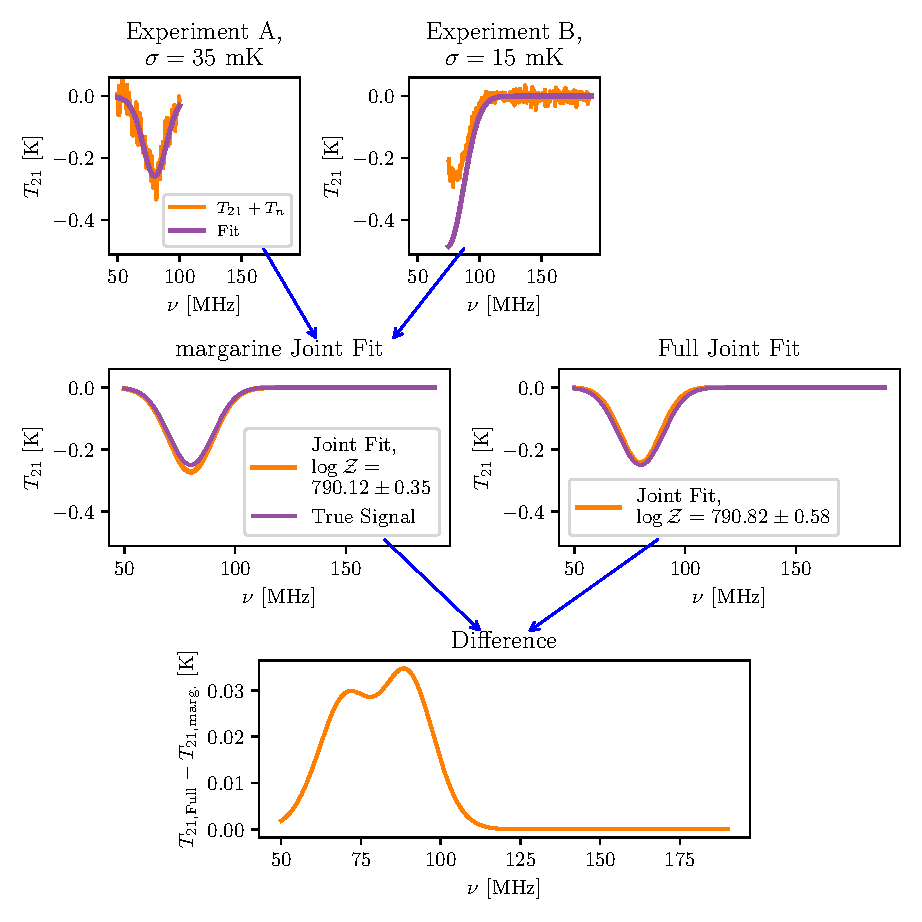
\includegraphics{margarine/figs/margarine_combined_signal.pdf}
    \caption{The top panels in the graph shows two simulated data sets comprising noise and a 21-cm signal as orange lines. In the same panels in purple, we show the averages of the functional posteriors derived from Nested Sampling fits to both of these data sets. Neither fit recovers the true signal exactly, however when we analytically combine the full likelihoods for each experiment, including foregrounds, and jointly fit the data we get a much better agreement across the whole frequency range as can be seen in the center right panel. We show the results of this joint analysis as a purple line. For comparison, we show in the center left panel, as an orange line, the average of the functional posterior from a joint fit performed with \textsc{margarine} using the nuisance-free likelihood function. We can see that the joint fits are equivalent, more accurate than the fits to each individual experiment and the Bayesian evidences are similar in magnitude when using the full likelihood and the nuisance-free likelihood. We show the difference between the two fits in the bottom panel as a function of frequency.}
    \label{fig:joint_likelihood}
\end{figure}

In this case because the problem is trivial sampling over $\theta$, $\alpha_A$ and $\alpha_B$ is not an inefficient or complex process, however generally speaking there are many more nuisance parameters that need to be modelled and the complexity of those models can significantly increase the evaluation time per call to the likelihood \citep[e.g. \cref{ch:saras2}, ][]{Bevins_SARAS2_2022}. In these circumstances, \textsc{margarine} can act as a useful tool for efficiently combining constraints from different data sets \citep[e.g. \cref{ch:hera_saras3}, ][]{Bevins_hera_saras3_2023} and this is discussed further in the next section.

\subsubsection{Combining constraints from Planck and DES}
\label{sec:results}

%It has previously been demonstrated that \textsc{margarine} is capable of replicating complex probability distributions and approximating marginal Bayesian statistics such as the KL divergence and the BMD \cite{margarine_neurips}. Here we demonstrate the theory discussed in \cref{sec:theory} by 
Here we combine samples from the Dark Energy Survey~(DES) Year 1 posterior \cite{DES_Year1_2018} and Planck posterior \cite{Planck2018} using \textsc{margarine} to estimate nuisance-free likelihoods. DES surveys supernovae, galaxies and large scale cosmic structures in the universe in an effort to measure dark matter and dark energy densities and model the dark energy equation of state. In contrast, Planck mapped the anisotropies in the Cosmic Microwave Background~(CMB) and correspondingly provided constraints on key cosmological parameters.

The constraints from DES and Planck have previously been combined using a full Nested Sampling run over all parameters including a multitude of `nuisance' parameters in a computationally expensive exercise \cite{Handley_tensions_2019} (e.g. \cref{fig:pipeline}). %This corresponds to the flow chart in \cref{fig:pipeline} and 
The previous analysis gives us access to the combined DES and Planck evidence, which is found to have a value of $\log(\mathcal{Z}) = -5965.7 \pm 0.3$. In \cref{fig:joint} we show the DES, Planck and joint posteriors for the six cosmological parameters derived in this work using \textsc{margarine} and the flow chart in \cref{fig:pipelineB}. The constrained parameters are the baryon and dark matter density parameters, $\Omega_b h^2$ and $\Omega_c h^2$, the angular size of the sound horizon at recombination, $\theta_{MC}$, the CMB optical depth, $\tau$, the amplitude of the power spectrum, $A_s$, and the corresponding spectral index, $n_s$. These make up the set $\theta = (\Omega_b h^2, \Omega_c h^2, \theta_{MC}, \tau, A_s, n_s)$. We use the Nested Sampling algorithm \textsc{polychord} in our analysis \cite{Handley2015a, Handley2015b}.

We use a uniform prior that is defined to be three sigmas around the Planck posterior mean. This is done to improve the efficiency of our Nested Sampling run. However, we subsequently have to re-weight the samples and correct the evidence for the difference between the priors used here and in the previous full Nested Sampling run \cite{Handley_tensions_2019} for comparison. If we define
\begin{equation}
    \mathcal{Z}_A = \int \mathcal{L}(\theta) \pi_A(\theta) d\theta, \qquad
    \mathcal{Z}_B = \int \mathcal{L}(\theta) \pi_B(\theta) d\theta, 
\end{equation}
where $A$ is our uniform prior space and $B$ is our target prior space from the previous work \cite{Handley_tensions_2019}, then
\begin{equation}
    \mathcal{Z}_B 
    = \int \mathcal{L}(\theta) \pi_B(\theta) d\theta
    = \int \mathcal{L}(\theta) {\pi_A(\theta)}\frac{\pi_B(\theta)}{\pi_A(\theta)} d\theta 
   = \mathcal{Z}_A\left\langle \frac{\pi_B(\theta)}{\pi_A(\theta)}\right\rangle_{\mathcal{P}_A}
\end{equation}
giving
\begin{equation}
    \mathcal{Z}_B 
    = \mathcal{Z}_A\left\langle \frac{\pi_B(\theta)}{\pi_A(\theta)}\right\rangle_{\mathcal{P}_A}.
\end{equation}
Then following similar arguments we can transform our posteriors by re-weighting the distributions with the following
\begin{equation}
    w^{(i)}_B 
    = w^{(i)}_A  \frac{\pi_B(\theta^{(i)})}{\pi_A(\theta^{(i)})}.
\end{equation}

We see from the figure and corresponding table that with our joint analysis we are able to derive a log-evidence that is approximately consistent with that found in \cite{Handley_tensions_2019}, $\log(\mathcal{Z}) = -5965.7 \pm 0.3$ as previously reported, further validating the theory discussed and its implementation with \textsc{margarine}. %We note that the re-weighting described above relies on calculation of the two prior log-probabilities for which we use \textsc{margarine} and currently do not have an estimate of the error for. As a result, the error in the combined evidence, $Z_B$, is given by the error in $Z_A$ from the nested samples and is likely underestimated. 
Using \textsc{margarine} we can also derive the combined KL divergence, also reported in \cref{fig:joint} and discussed further in this chapter, which we find is consistent with the result in the literature of $\mathcal{D} = 6.17 \pm 0.36$ \cite{Handley_dimensionality_2019}. Similarly, we derive marginal KL divergences for the DES and Planck cosmological parameters using \textsc{margarine} (the DES example is furthered in the following subsections). A full discussion of the implications of combining the two data sets for our understanding of cosmology can be found in the literature \cite[e.g][]{Handley_tensions_2019, Handley_dimensionality_2019}.

By reducing the number of parameters that need to be sampled, we significantly reduce the Nested Sampling runtime. For \textsc{polychord} the runtime scales as the cube of the number of dimensions \cite{supernest}. This can be seen by assessing the time complexity of the algorithm where, $T \propto n_\mathrm{live} \times \langle T\{\mathcal{L}(\theta)\}\rangle \times \langle T\{Impl.\}\rangle \times \mathcal{D}(\mathcal{P}||\pi)$. Here $n_\mathrm{live}$ scales with the number of dimensions, $d$, as does the Kullback-Leibler divergence. For \textsc{polychord}, the specific implementation time complexity factor, $\langle T\{Impl.\}\rangle$, representing the impact of replacing dead points with higher likelihood live points on the runtime, scales linearly with $d$. Together this gives $T \propto d^3 \times \langle T\{\mathcal{L}(\theta)\}\rangle$. Therefore, by using nuisance-free likelihoods and sampling over 6 parameters rather than 41 parameters (cosmological plus 20 nuisance parameters for DES and 15 different nuisance parameters for Planck) we reduce the runtime by a factor of $(41/6)^3 \approx 319$ with further improvements in $\langle T\{\mathcal{L}(\theta)\}\rangle$. %Using \textsc{margarine}, $\langle T\{\mathcal{L}(\theta)\}\rangle$ is typically reduced since analytic likelihoods are computationally more expensive than emulated likelihoods.

\begin{figure}
    \centering
    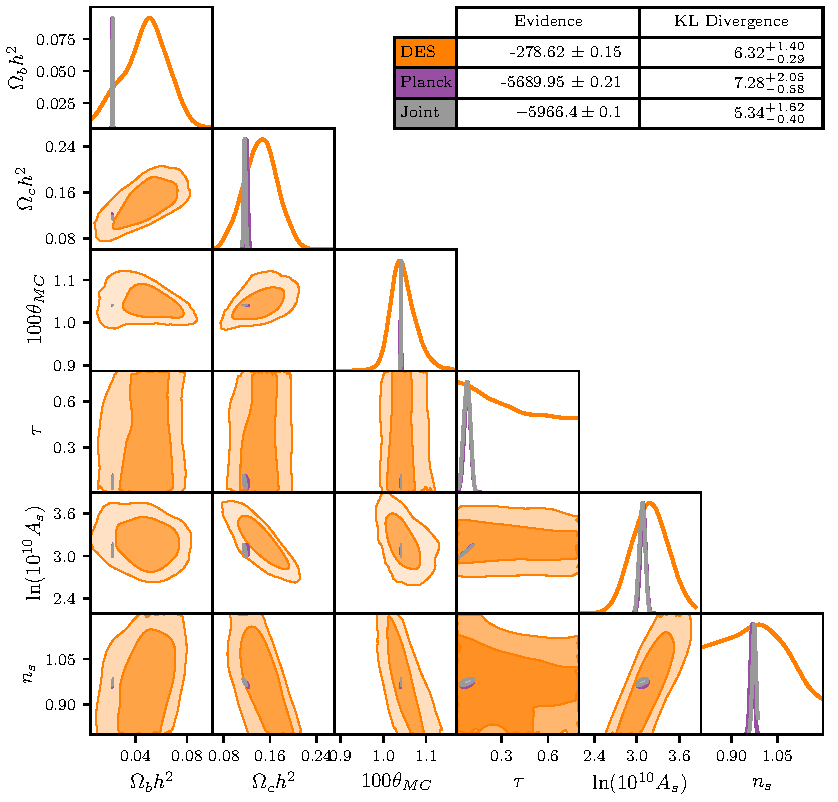
\includegraphics{margarine/figs/paper_plot.pdf}
    \caption{The combined posterior (in grey) found when combining the constraints on the cosmological parameters from DES and Planck using \textsc{margarine}. For DES and Planck, we calculate the marginal KL divergences using \textsc{margarine}, whereas the Bayesian evidences are calculated using \textsc{anesthetic}. The joint evidence and joint KL divergence are calculated with a combination of the two codes and are found to be approximately consistent with those found in the literature \cite{Handley_tensions_2019, Handley_dimensionality_2019}. Note that the error on the joint evidence is likely underestimated as it relies on evaluations of log-probabilities for various distributions, for which \textsc{margarine} does not currently provide errors. The figure produced with \textsc{anesthetic} \cite{anesthetic}.}
    \label{fig:joint}
\end{figure}

\subsection{Prior Emulation}

Since the 21-cm signal is dependent on many different astrophysical process, semi-numerical simulations can take several hours to produce a single model. This is impractical if we want to use Bayesian inference techniques like MCMC and Nested Sampling algorithms to fit real data. Signal emulators, like those discussed in the previous chapter, are often used as a fast alternative that can accurately model the relationship between the astrophysics and the signal structure and produce signal realisations in 10s of milliseconds. An even cheaper alternative is to approximate the signal with a Gaussian absorption feature, as alluded to in the previous section. However, it is not always clear how to set the priors on the parameters $T_\mathrm{min}$, $\nu_c$ and $\Delta \nu$ in \cref{eq:gaussian_signal}. For this, we can use \textsc{margarine}.

The idea here is to take a large set of physically motivated signals generated using an emulator from a uniformly sampled prior on the astrophysical parameters describing the underlying semi-numerical simulation. For each physical signal we then calculate the depth corresponding to $T_\mathrm{min}$, the central frequency $\nu_c$ and approximate the width $\Delta \nu$. Through this process we arrive at a physically motivated set of samples in the phenomenological parameters which we can train a MAF on using \textsc{margarine}, creating a physically motivated prior on our phenomenological parameters.

We use the global 21-cm signal emulator \textsc{globalemu} \citep{Bevins_globalemu_2021}, discussed in \cref{ch:globalemu}, to model a set of 5,000 signals based on a parameterisation of the signal that includes; $V_c$ the minimum virial circular velocity that is proportional to the cube root of the halo mass for star formation, $f_*$ the star formation efficiency, $f_X$ is the X-ray production efficiency which is proportional to the X-ray luminosity, $\tau$ the CMB optical depth and $f_r$ the radio production efficiency proportional to the radio luminosity \cite{Reis2020}.
Whilst 5,000 signals may seem like a large number of models, the equivalent number generated in a Nested Sampling or MCMC run would be far larger.

In scenarios with poor star formation, corresponding to high $V_c$ and low $f_*$, and large X-ray heating corresponding to high $f_X$ we find that the signal cannot be well approximated by a Gaussian profile because it features a weak absorption feature and strong emission. We therefore filter out these scenarios before training our MAF and of the 5,000 models we initially started with, 87\% are used to produce our physically motivated prior. In \cref{fig:physical_prior} we show the distribution on $\log_{10}(|T_\mathrm{min}|)$, $\nu_c$ and $\Delta \nu$ generated from the physical models and samples from the corresponding MAF which can be used as a prior on the Gaussian model.

In 21-cm cosmology, instrumental effects can introduce non-smooth structure to the data. These effects are often sinusoidal \citep[e.g.][]{Bevins_maxsmooth_2021, Bevins_SARAS2_2022} and if not corrected for they can affect the recovery of the 21-cm signal. For example, part of a damped sinusoidal structure in the data with a periodicity of 5~MHz can be modelled with the approximate Gaussian signal profile discussed in this chapter if the prior on the width is wide. However, from \cref{fig:physical_prior} we see that a signal profile of width 5~MHz is not likely to represent a physical scenario. The goal of the physically motivated prior is to therefore provide some information about the anticipated signal that can help to separate it from and prevent fitting systematic structures in the data when using a Gaussian profile for the signal.

\begin{figure*}
    \centering
    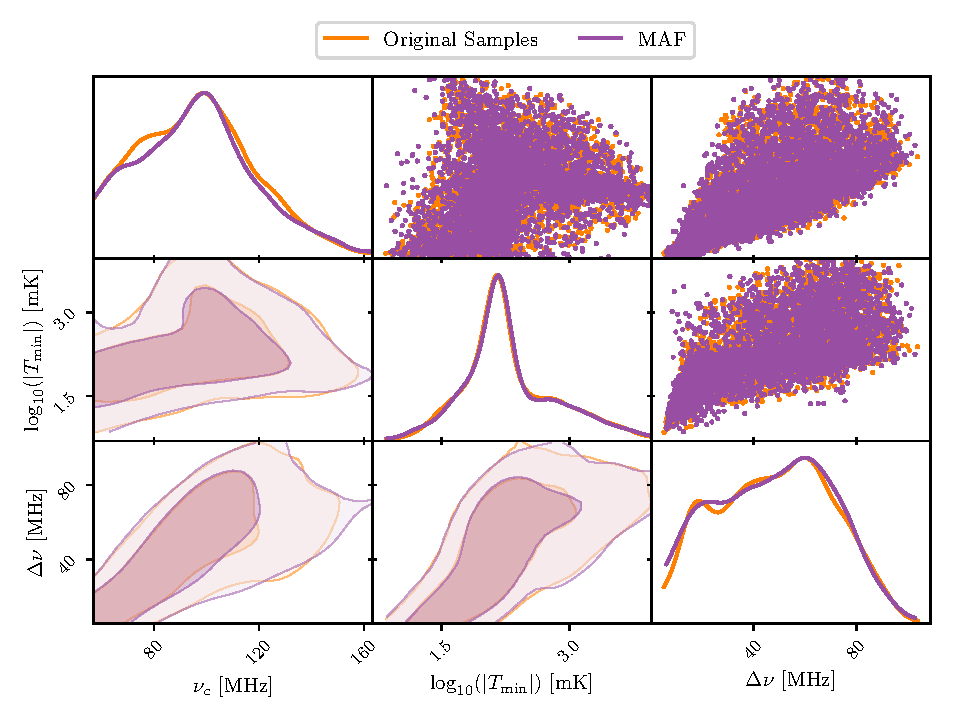
\includegraphics{margarine/figs/physical_prior_example.pdf}
    \caption{A physically motivated prior on the phenomenological parameters of a Gaussian absorption feature used to model the sky-averaged 21-cm signal. $\nu_c$ is the central frequency of the absorption feature, $T_\mathrm{min}$ is the corresponding temperature, and $\Delta \nu$ is the approximate width of the 21-cm signal. The prior is derived by approximating the phenomenological parameters for a set of physically motivated signals generated with a neural network emulator and learning the corresponding distribution, in orange, with a MAF. Samples from the MAF are shown in purple.}
    \label{fig:physical_prior}
\end{figure*}

\subsection{Marginal Bayesian Statistics}
\subsubsection{Toy Example Posteriors}

We use two different toy examples for which we know the KL divergence and BMD to demonstrate the calculation of marginal Bayesian statistics. We sample the example Gaussian likelihoods, both with five parameters, using \textsc{polychord}, and we show the corresponding distributions in orange in \cref{fig:toy_example}. The first has a series of correlations between the parameters (left-hand panel) and the second has a combination of uncorrelated parameters with both log-uniform and uniform priors on the parameters (right-hand panel).

\begin{figure*}
    \centering
    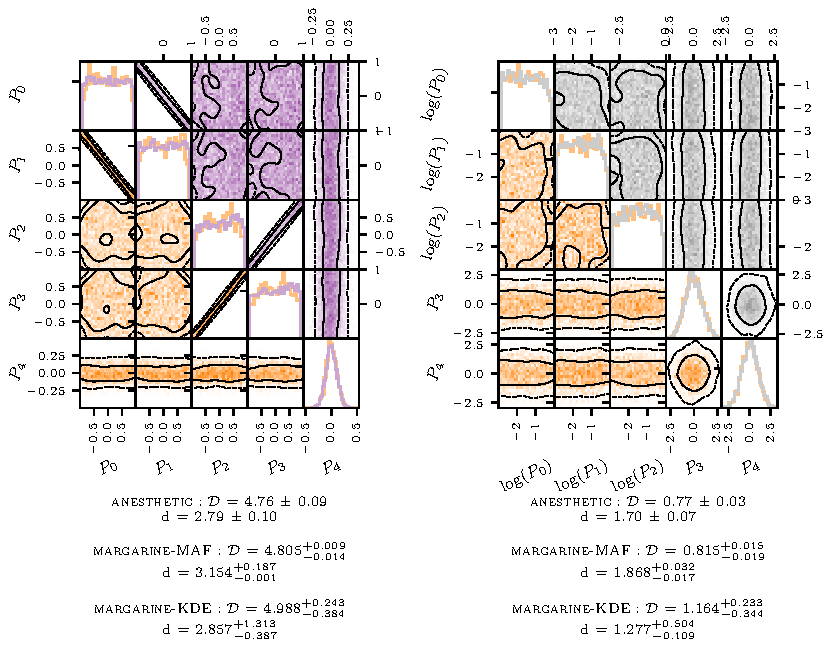
\includegraphics[width=\linewidth]{margarine/figs/toy_examples_alt.pdf}
    \caption{\textbf{Left Panel:} The graph shows a set of correlated nested samples from \textsc{polychord} in orange along with a reconstruction from a trained KDE in purple. Listed are the corresponding `true' values for the KL divergence and BMD from \textsc{anesthetic} and the estimated values from \textsc{margarine} using both a KDE and MAF. \textbf{Right Panel:} An equivalent graph for a set of uncorrelated samples with both log-uniform and uniform priors on the parameters, shown in orange. The gray samples are taken from a trained MAF, and we report the `true' Bayesian statistics values from \textsc{anesthetic} along with estimates calculated using a MAF and KDE with \textsc{margarine}.}
    \label{fig:toy_example}
\end{figure*}

We are able to use the samples from \textsc{polychord} and the analysis tool \textsc{anesthetic}~\cite{anesthetic} to calculate the KL divergence and BMD for both toy examples and these values are reported, with errors, in \cref{fig:toy_example}. We show samples drawn from a KDE trained on the correlated samples and from a MAF trained on the uncorrelated samples, with values of $\mathcal{D}$ and $d$ listed for both types of density estimator.

The errors in $\mathcal{D}$ and $d$ are estimated by propagating both samples generated with the density estimator and the original samples through the density estimator to evaluate the log-probabilities and comparing the resultant statistics. If the density estimator is a perfect representation of the original distribution, then we would expect samples drawn from it to be from the same distribution as the original samples. This would lead to an approximate equivalence between the two sorted log-probability distributions as functions of the sorted associated Nested Sampling weights~\cite{Harrison2015} and so any deviation we see gives us an indication of the error in our marginal statistics.

For the correlated samples, we see that the estimated KL divergence and BMD from the MAF and from the KDE are in close agreement with the `true' value output from \textsc{anesthetic}.
For the uncorrelated samples, we also see that the MAF KL divergence and BMD estimates are in agreement with the \textsc{anesthetic} values. For the KDE, the KL divergence and BMD are less consistent with the values from the MAF and from \textsc{anesthetic}, however we find we have larger errors when using the KDEs likely because they are less expressive than the MAFs. 

Typically, the upper and lower bounded range on the BMD estimates are larger than for the KL divergence estimates because it has a more complex dependence on $\log\mathcal{L}$. Future work is needed to investigate whether improvements can be made to the BMD estimates by modifying the MAF loss function, network configurations or KDE bandwidths among other tunable parameters.

\subsubsection{Radio Experiment for the Analysis of Cosmic Hydrogen}

%The Radio Experiment for the Analysis of Cosmic Hydrogen~(REACH) is an experiment aiming to detect the sky-averaged 21-cm signal in the frequency range $50 - 170$ MHz.

The Radio Experiment for the Analysis of Cosmic Hydrogen~(REACH)  data analysis pipeline \cite{Anstey_REACH_2021} uses Nested Sampling, implemented with \textsc{polychord}, to model the different components of the data. The pipeline has been extensively tested on mock observations~\citep{Anstey_REACH_2021,Anstey_antenna_2022,Cumner_antenna_2021, Scheutwinkel2022a, Scheutwinkel2022b}. We generate mock observational data using a realistic foreground model derived from an all-sky map and inject a Gaussian signal profile with an amplitude of $|T_\mathrm{min}| = 155$~mK, a central frequency of $\nu_c = 85$~MHz and a standard deviation of $\Delta \nu = 15$~MHz.

The mock data correspond to a single snapshot observation taken from the Karoo radio observatory with a dipole antenna and modelled with a foreground model that takes advantage of the spectral structure of the sky, a correction for the non-uniform response of the antenna to the sky, Gaussian noise and a Gaussian signal profile corresponding to a 16 dimensional parameter space. In the left-hand panel of \cref{fig:cosmo_examples} we show the posterior distribution for the signal parameters from our fit in orange, having marginalised over the other 13 parameters, and the corresponding KDE reconstruction from \textsc{margarine} is shown in purple. We see a reasonable consistency between the marginal KL divergence calculated for these samples when using both the KDE and MAF. 

However, we note that there are some differences in the BMD estimate, with the MAF giving a larger value for $d$. From a visual inspection of the samples we would expect the BMD to be around 1-2 due to the tight constraint on $\nu_c$ and weaker but still non-trivial constraint on $|T_\mathrm{min}|$ meaning that both estimates are somewhat consistent with expectations.

\begin{figure*}
    \centering
    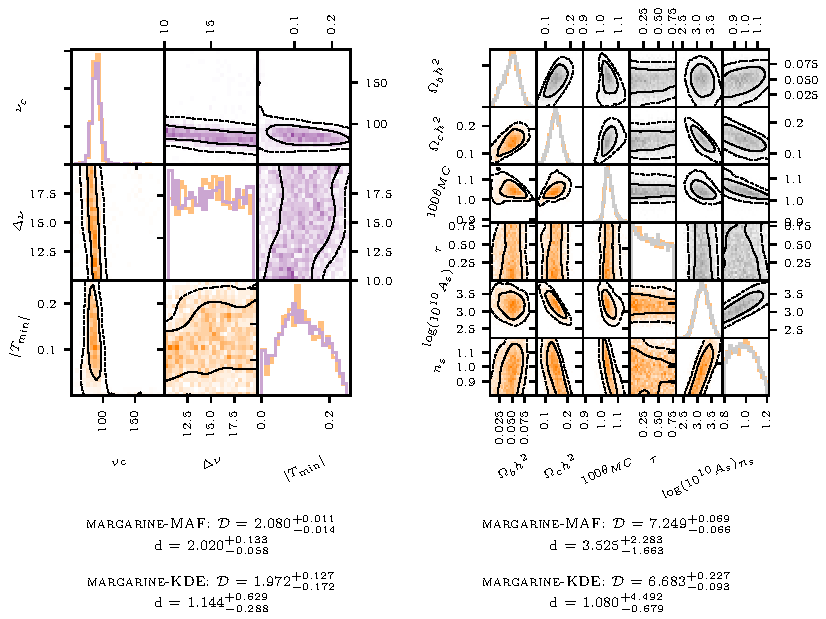
\includegraphics[width=\linewidth]{margarine/figs/cosmo_examples_alt.pdf}
    \caption{\textbf{Left Panel:} The signal subspace, in orange, for a fit to simulated observations of the 21-cm signal with the REACH experiment along with samples, in purple, from KDE trained on the three signal parameters effectively marginalising over the other thirteen parameters in the fit. We report the marginal KL divergence and BMD found for this set of three parameters using both a MAF and KDE. \textbf{Right Panel:} The cosmological subspace for the Year 1 DES samples shown in orange, along with a set of samples taken from a trained MAF in gray. Again, we report the corresponding marginal Bayesian statistics calculated with \textsc{margarine}.}
    \label{fig:cosmo_examples}
\end{figure*}

\subsubsection{Dark Energy Survey}

%The Dark Energy Survey~(DES) is designed to help us understand why the Universe's rate of expansion is accelerating. The goal of the collaboration is to map millions of galaxies, thousands of supernova and large scale cosmic structures in order to help understand the dark energy which makes up 70\% of the universe. The survey has targeted the measurements of the dark matter and dark energy densities as well as the dark energy equation of state~\cite{DES_2005} by investigating galaxy clustering, gravitational lensing and supernova distances.

The Year 1 DES analysis\footnote{We note that the Year 3 DES results have been published~\cite{DES_year3, DES_year3_2021} but that the samples have not been made publicly available.} \cite{Handley_tensions_2019}, as discussed, aimed to constrain the baryon density parameter, $\Omega_b$, the dark matter density parameter, $\Omega_c$, the approximate ratio of the sound horizon to the angular diameter distance, $\theta_{MC}$, the optical depth of the CMB to reionization, $\tau$ and the amplitude and tilt of the power spectrum, $A_s$ and $n_s$. The samples from the cosmological subspace are shown in orange in the right-hand panel of \cref{fig:cosmo_examples}, where we have marginalised over a set of 20 nuisance parameters, along with a MAF reconstruction of the subspace in gray.

Unlike the toy examples and REACH samples, the DES cosmological samples do not have uniform priors and cannot easily be transformed into a space in which the priors are uniform. As a result, we have to use the density estimators built into \textsc{margarine} to evaluate both the log-probability of the posterior and the prior if we want to calculate marginal statistics.

While this is possible, it is expected to lead to an increased uncertainty in the marginal statistics, which can be seen in \cref{fig:cosmo_examples}. In addition, the problem is further complicated by the size of the cosmological parameter space, since we expect larger parameter spaces to be harder to replicate well with \textsc{margarine}, and consequently we expect larger errors on the marginal statistics.

Again the density estimators give us different estimates for the BMD, however the errors are large. From a visual examination of the distribution, we would expect the BMD to be between $\approx3$ and $\approx4$. There is a reasonable agreement between the KL divergence calculated for the cosmological constraints from DES with both the MAF and the KDE. We note that the KL divergence reported here for the DES samples is different from that reported in \cref{fig:joint} but that the two estimates are consistent with each other. The difference stems from the fact that in each analysis we retrained the DES MAF.

\section{Conclusions}
\label{sec:conclusions_margarine}

In this chapter we have demonstrated a number of applications of two different types of density estimator, Masked Autoregressive Flows and Kernel Density Estimators, to the calculation of marginal Bayesian statistics, the efficient modelling of multiple data sets and the derivation and emulation of physical priors. \textsc{margarine} is a multipurpose tool that can be used to enhance our Bayesian analysis workflows.

The evaluation of marginal KL divergences and Bayesian Model Dimensionalities allows for improved comparison of the constraining power of different experiments targeting the same astrophysical or cosmological signals with different systematics or nuisance parameters. In turn, this can lead to improvements in experimental design with techniques that provide more information about the signals of interest being pursued in the future. The calculation of marginal Bayesian statistics has been illustrated in \cite{Scheutwinkel2022b}, \cite{Anstey_lst_2022} and \cref{ch:saras3} \cite{Bevins_saras3_2022}.

The nuisance-free likelihood function allows for more efficient combination of constraints from different data sets, preventing the need to sample instrument specific foreground and systematic effects in joint analysis. This was demonstrated with data from the Planck and Dark Energy Survey experiments, and is explored further with data from the 21-cm power spectrum experiment HERA and sky-averaged 21-cm experiment SARAS3 in \cref{ch:hera_saras3} \citep{Bevins_hera_saras3_2023}.

Finally, \textsc{margarine} can be used to generate non-trivial priors (e.g. \cite{Alsing_bijectors_2021}) either from experimental results or simulations, as illustrated in this chapter. In principle, this allows us to inform the analysis of data from upcoming probes like REACH \citep{de_lera_acedo_reach_2022} or the Simons Observatory \citep{Simons_Obs_2019, Simons_obs_2019b} with results from existing experiments like SARAS3 \citep{Bevins_saras3_2022} and Planck \citep{Planck2018}. We anticipate further development of \textsc{margarine} and additional unexpected applications that evolve as the code is used.


\part{Applications to Real Data}

In this section, we apply the tools outlined in the previous chapters to real data from the global 21-cm signal experiments SARAS2 and SARAS3 and the power spectrum experiment HERA. The work builds on the current experimental results outlined in \cref{sec:current_results} and makes significant use of Bayesian analysis techniques outlined in \cref{sec:bayesian_inference_intro}.

In \cref{ch:saras2}, we analyse data from the SARAS2 instrument in the redshift range $z\approx7-12$ corresponding to the epoch of reionization. We identify the presence of a sinusoidal systematic in the data and model this alongside a maximally smooth foreground (see \cref{ch:maxsmooth}) and several different signal models which are emulated with \name~(see \cref{ch:globalemu}). The work is based on the first author paper \cite{Bevins_SARAS2_2022} published in Monthly Notices of the Royal Astronomical Society.

We follow this with an analysis of data from the SARAS3 instrument corresponding to $z\approx 15-25$ and the cosmic dawn when the first stars form. In this work, we produce the best constraints to date on the properties of the first stars using emulation of semi-numerical signals with \name. This chapter is based on the first author paper \cite{Bevins_saras3_2022} which was published in Nature Astronomy.

Finally, in \cref{ch:hera_saras3}, we demonstrate, using \textsc{margarine}~(see \cref{ch:margarine}), how a combined analysis of data from the power spectrum experiment HERA and data from the global signal experiment SARAS3 can lead to improved constraints in comparison to analysis of the individual data sets. This chapter is based on \cite{Bevins_hera_saras3_2023}.

\chapter{Constraints on the properties of galaxies between $z\approx7-12$ with SARAS2}
\label{ch:saras2}
\section{Introduction}
\label{sec:intro_saras2}

Several experiments, both single antenna and interferometers, have provided constraints on the parameter space of the 21-cm signal at redshifts corresponding to the EoR including HERA~ \citep{HERA_2022b}, LOFAR ~\citep{Ghara_LOFAR_2020, Mondal_LOFAR_2020, Greig_LOFAR_2021}, MWA ~\citep{Greig_MWA_2020, Ghara_MWA_2021}, EDGES ~\citep{Monsalve_EDGES_HB_1_2017, Monsalve_EDGES_HB_2_2018, Monsalve_EDGES_HB_3_2019} and SARAS2 ~\citep{Singh_saras2_2017, Singh_saras2_2018}.
We note that the parameterisation and modelling of the signals, as well as the prior ranges, are not always consistent across the literature. However, in general the conclusions disfavour signals with deep absorption features, within the band of each instrument, from inefficient X-ray heating and a sharp reionization feature.

In this chapter, we present a re-analysis of the SARAS2 data, which targeted the EoR at low redshifts (high frequencies). Previous analysis of 63 hrs of nighttime observations, between October 2016 and July 2017, at the Timbaktu Collective in Southern India with the SARAS2 instrument concluded that scenarios with rapid reionization and weak X-ray heating were disfavoured by the data \citep[][]{Singh_saras2_2017, Singh_saras2_2018}. In this analysis, the authors used a Bayesian likelihood ratio test to determine whether the presence of particular signal models, from a simulated set of 264, were favoured in the data or not \citep{Singh_saras2_2017}. This was followed by a detailed frequentist approach that ruled out a larger number of simulated signals from the same set of models and using the same data \citep{Singh_saras2_2018}. Of the tested scenarios, 9 were disfavoured by the data in \cite{Singh_saras2_2017} and 20, of which 15 were rejected with a significance $> 5\sigma$, were rejected in \cite{Singh_saras2_2018}. There was no reported detection from the analysis. In both cases high order polynomials were used to model the foreground and systematics, in the belief that any present in the data are smooth, in combination. A high level summary of the differences between the analysis in this chapter and the previous analysis of the SARAS2 data can be found in \cref{tab:high_level_summary} and these are further discussed below.

We determine parameter constraints over broad prior ranges using the latest astrophysical models of the global 21-cm signal \citep{Reis2020, Reis_sta_2021}, representing an improved understanding of the standard astrophysical picture, and the Nested Sampling algorithm \citep{skilling_nested_2004} \textsc{polychord} \citep{Handley2015a, Handley2015b}. We use models that include Lyman-$\alpha$ heating~\citep{Madau1997, chen_lah_2004, furlanetto_scattering_2006, Chuzhoy2007}, CMB heating~\citep{Venumadhav2018} and multiple scattering of Lyman-$\alpha$ photons \citep{semelin_b_lyman-alpha_2007, Naoz2008, baek_s_simulated_2009, visbal_impact_2018, molaro_artist_2019, reis_mapping_2020}. The effects on the global signal of these physical processes have been understood for some time, but the magnitude of those effects over a larger parameter space were not understood until recently \citep{Villanueva2020, Mittal2021, Reis_sta_2021}. Additionally, we study astrophysical scenarios with a wide range of radio production efficiencies, $f_\mathrm{radio}$, for early galaxies. A subset of the latter models could explain the anomalous EDGES detection \cite{Bowman_edges_2018} using an excess radio background. This is the first time that a full Bayesian analysis of data from a global 21-cm experiment has been performed with these specific astrophysical simulations. We note, however, that the value of $f_\mathrm{radio}$ has previously been constrained using the amplitude of the EDGES absorption feature \citep{Reis2020} and more recently using upper limits on the power spectrum from the Hydrogen Epoch of Reionization Array~\citep[HERA,][]{HERA_2022b} \footnote{The updated HERA constraints precented in \cite{HERA_2022c} were published after the paper associated with this chapter.}.

In this work we use the emulator \textsc{globalemu} \citep[see \cref{ch:globalemu}, ][]{Bevins_globalemu_2021} which we train on sets of signal models from \cite{Reis2020} and \cite{Reis_sta_2021}. %It has been shown that global signal emulators such as \textsc{21cmGEM} \citep{Cohen2020} can be used for quick interpolation of the signal across the astrophysical parameter space \citep{Monsalve_EDGES_HB_3_2019}. \textsc{globalemu} is a flexible framework that can easily learn different simulations of the global signal and has been shown to be faster and more accurate than the previous state of the art \citep{Cohen2020}. 
We provide more details on the accuracy of each trained instance of \textsc{globalemu} in \cref{sec:signal_modelling}.

\begin{landscape}
\begin{table*}
    \centering
    \begin{tabular}{|c|p{3cm}|p{4cm}|p{5cm}|}
        \hline
         & Singh et al. 2017\cite{Singh_saras2_2017} & Singh et al. 2018 \cite{Singh_saras2_2018} & This work \\
         \hline
         \hline
         Analysis Type & Likelihood ratios testing preference of the data for the presence or absence of signals. & Frequentist approach based on that used in \cite{Monsalve_EDGES_HB_1_2017}. & Bayesian Nested Sampling using \textsc{polychord} \citep{Handley2015a, Handley2015b}. \\
         \hline
         Foreground Modelling & \multicolumn{2}{p{8cm}|}{Unconstrained polynomials of varying orders (e.g. N = 4 -8 in \citep{Singh_saras2_2018}).} & Smooth foreground models based on Maximally Smooth Functions and implemented with \textsc{maxsmooth} \citep{Bevins_maxsmooth_2021}. \\
         \hline
         Systematic Modelling & \multicolumn{2}{l|}{Assumed to be smooth and modelled with foreground model.} & Identified through use of smooth foreground model and separately modelled with physically motivated functions. \\
         \hline
         Noise Modelling & \multicolumn{2}{l|}{Gaussian distributed noise based on system attributes.} & A set of Gaussian models with constant, frequency damped and relative weights based amplitudes.\\
         \hline
         Signal Modelling & \multicolumn{2}{p{8cm}|}{A library of 264 standard astrophysical models with no additional radio background above the CMB~\citep{Cohen_global_2017}.} & Broader study sampling across large prior ranges, for both standard astrophysical models \citep{Reis_sta_2021} and exotic astrophysical models with excess radio backgrounds \citep{Reis2020}, using the signal emulator \textsc{globalemu} \citep{Bevins_globalemu_2021}. \\
         \hline
    \end{tabular}
    \caption{A high level summary of the differences between the previous analysis of the SARAS2 data and the work performed in this chapter. The differences are expanded on primarily in \cref{sec:modelling}.}
    \label{tab:high_level_summary}
\end{table*}
\end{landscape}

We illustrate the presence of a sinusoidal systematic in the data and attempt to physically model the structure in a manner which is independent of the foreground model. We use two separate models, each representing the introduction of a systematic at different points in the SARAS2 experiment. The motivation for each model is explained in \cref{sec:systematic modelling}.

The identification of the systematic is driven by the application of \textsc{maxsmooth} \citep[see \cref{ch:maxsmooth}, ][]{Bevins2020, Bevins_maxsmooth_2021} to model the foreground and smooth systematics in the data with a model that has constrained derivatives and resultant smooth properties based on Maximally Smooth Functions \citep[MSFs, ][]{Sathyanarayana2015, Sathyanarayana_msf_2017}. The motivation behind the use of \textsc{maxsmooth} is two-fold. Firstly, the SARAS2 antenna is designed and has been shown to have a maximally smooth reflection coefficient and efficiencies \citep{SARAS2_radiometer_2018}. Secondly, the dominant foregrounds in global 21-cm experiments from Galactic and extragalactic synchrotron and free-free emitting sources are expected to be smooth power laws \citep{Sathyanarayana_msf_2017, Bernardi_galaxy_2009, Nitu_background_2021}.

In \cref{sec:data} we discuss briefly the SARAS2 experiment and the data that we are analysing. This is followed by a more detailed description of the modelling that we perform in \cref{sec:modelling}, a discussion about the sensitivity of the data to specific models in \cref{sec:sensitivity} and a summary of our results in \cref{sec:results_saras2}. We draw conclusions in \cref{sec:saras2_conclusions}.

Eloy de Lera Acedo, Anastasia Fialkov, Will Handley, Saurabh Singh, Ravi Subrahmanyan and Rennan Barkana provided comments on \cite{Bevins_SARAS2_2022} which formed the basis of this chapter.

\section{The SARAS2 data}
\label{sec:data}

One of the primary causes of systematics in global 21-cm experiments is chromaticity in the typically very wide beam pattern of the antenna. Sidelobes in the antenna beam, complex reflection coefficients and environmental factors can introduce frequency dependent structures in the data. However, we can attempt to build achromatic smooth antennas and this is the motivation behind the design of the SARAS2 antenna, which is a short monopole designed to have a smooth beam. 

In principle, the foreground and systematics in the data from the SARAS2 experiment should both be smooth, and significant efforts were made to ensure that the efficiency and reflection coefficients in the data were smooth functions \citep{SARAS2_radiometer_2018}. This has been explored in \cite{Sathyanarayana_msf_2017} where it was shown that simulated observations with the SARAS2 antenna of the foregrounds \citep[produced with the Global Model for the Radio Sky Spectrum,][]{Sathyanarayana2016} are smooth in structure to within a few mK. This is also expected generally, in the absence of ionospheric effects \citep{Shen_ionosphere_2021}, for an achromatic beam like SARAS2.

SARAS2 was deployed in the remote radio quiet Timbaktu Collective in Southern India (lat = + 14.$^{\circ}$242328, long = 77.$^{\circ}$612606E). The antenna comprised of a sphere mounted on top of an inverted cone resting on a circular aluminium disk. The components are smoothly joined and placed above the receiver electronics at the site. The electronics are battery powered and the site is flat and open. An optical fiber is used to connect the receiver to a signal processing unit situated 100~m away.

The beam pattern of the SARAS2 antenna is simulated, measured and shown to be frequency independent \citep{SARAS2_radiometer_2018}. The pattern is omnidirectional and constant in azimuth, with nulls at zenith and horizon, a peak at 30 degrees in elevation and a half-power beam width of 45 degrees in elevation. A 3D visualisation can be found in Fig. 8 of \cite{Sathyanarayana_msf_2017}. 

The antenna temperature, assuming the presence of a global 21-cm signal $T_{21}$, would correspond to
\begin{equation}
    T_\mathrm{A} = (T_{21} + T_\mathrm{gr} + T_\mathrm{fg})\eta_t,
\end{equation}
where $T_\mathrm{fg}$ accounts for the Galactic and extragalactic foregrounds and $\eta_t$ corresponds to the total efficiency of the SARAS2 antenna. $T_\mathrm{gr}$ refers to ground emission and for the analysis presented here we assume that the ground emission is smooth or equivalently that the ground under the antenna is homogeneous. As a result, we can subsume the ground emission term into our smooth foreground model and treat the antenna temperature as being given by
\begin{equation}
    T_\mathrm{A} = (T_{21} + T_\mathrm{fg})\eta_t.
    \label{eq:components}
\end{equation}
The assumption of a homogeneous ground under the antenna may not hold and that this may cause the introduction of non-smooth systematics into the data~(see \cref{sec:systematic modelling}). The sum $T_W = (T_{21} + T_\mathrm{fg})$ represents the beam-weighted sky power and $\eta_t$ is the product of the radiation and reflection efficiency \citep{SARAS2_radiometer_2018}. $\eta_t$ therefore, accounts for the loss due to an impedance mismatch between the antenna and the transmission line to the receiver, as well as the frequency dependent coupling of the beam-weighted sky temperature to the antenna. Estimates of $\eta_t$ are made using the Global Model for the Radio Sky Spectrum~(GMOSS simulations and measurements of the differential antenna temperature as the sky passes through the beam. The calibration and RFI rejection are detailed in section 6 of \cite{SARAS2_radiometer_2018} and summarised in \cite{Singh_saras2_2017}. We are assuming that the data has been calibrated to be in Kelvin units of antenna temperature and that there is no residual RFI.

The data can be seen in \cite{Singh_saras2_2017, Singh_saras2_2018} and we discuss the sensitivity of the data to the global 21-cm signal in \cref{sec:sensitivity} after introducing the signal models in the following section.

\section{Modelling}
\label{sec:modelling}

The Bayesian Nested Sampling tool \textsc{polychord} \citep{Handley2015a, Handley2015b} is used to fit two different systematic models and two different parametrisations of the global signal to the SARAS2 data. We model the foreground using the software \textsc{maxsmooth} \citep{Bevins2020, Bevins_maxsmooth_2021} and emulate physical models of the global signal with \textsc{globalemu} \citep[][]{Bevins_globalemu_2021}.

In practice, we model the foreground as $T_\mathrm{fg}^* = T_\mathrm{fg}\eta_t$. Throughout the rest of the chapter we generally assume, unless otherwise stated, that when discussing the foreground we are including in that definition $\eta_t$ and any additive smooth systematics. We consider the addition of non-smooth systematics, $T_\mathrm{NS}$, into \cref{eq:components} in \cref{sec:systematic modelling}. The details of the different components of our model are given in the following subsections. 

We briefly discuss the reproducibility of our results in Appendix A of \cite{Bevins_SARAS2_2022}.

\subsection{Noise Modelling}
\label{sec:noise_models}

\begin{table}
    \centering
    \begin{tabular}{|p{3cm}|p{2cm}|p{4cm}|p{3cm}|}
        \hline
        Noise Model & $\sigma$ & Prior & Prior Type \\
        \hline
        \hline
        Constant & $A_{\sigma}$ & $A_{\sigma}=10^{-3}-10^{-1}$ mK & Log Uniform\\
        \hline
        \multirow{2}{1.5cm}{Frequency Damped} & \multirow{2}{*}{$A_{\sigma}\bigg(\frac{\nu}{\nu_0}\bigg)^{-\beta_{\sigma}}$} & $A_{\sigma}=10^{-4}-10^{-1}$ mK & Log Uniform \\
        \cline{3-4}
        & & $\beta_{\sigma} = 0 - 5$ & Uniform \\
        \hline
         Relative Weights & $A_{\sigma}~W(\nu)$ & $A_{\sigma} = 10^{-2}-10^{-1}$ mK & Log Uniform\\
         \hline
    \end{tabular}
    \caption{The tested frequency dependent and independent standard deviation models for the assumed Gaussian noise in the SARAS2 data. In the frequency damped, noise model $\nu_0$ is the central frequency in the band. The origin of the relative weights, $W(\nu)$, is discussed in \cref{sec:noise_models}.}
    \label{tab:noise_models}
\end{table}

For all the fits performed in this chapter, we assume that the noise in the data is Gaussian distributed and use a Gaussian log-likelihood function
\begin{equation}
    \log\mathcal{L} = \sum_i \bigg(-\frac{1}{2}\log(2\pi\sigma^2) -\frac{1}{2}\bigg(\frac{T_\mathrm{A}(\nu_i) - T_\mathrm{M}(\nu_i)}{\sigma}\bigg)^2\bigg),
    \label{eq:likelihood}
\end{equation}
where $T_\mathrm{M}$ stands for the sum of the model components described below. %Our assumption is supported by assessment of the noise, which shows a Gaussian distribution, in data that has passed through the SARAS2 radiometer using a series of different terminations measured in the lab \citep{SARAS2_radiometer_2018}. 
Our assumption is supported by previous analysis of the data, which produced residuals with a Gaussian distribution after removing a high order polynomial model for the structure in the data \citep[see][]{Singh_saras2_2017, Bevins_SARAS2_2022}.

Typically, the noise is assumed to be frequency independent, however, in practice the noise is dependent on the system temperature which is dominated by the sky temperature and is a function of frequency. In this chapter we consider three different approximations to the standard deviation, $\sigma$, of the assumed Gaussian noise, each with a different frequency dependence. The first is a constant value of $\sigma$ and the second is given by a frequency damped amplitude. The latter comes from the naive expectation that $\sigma$ should be proportional to, $T_W$ which means that the standard deviation should decrease with increasing frequency following the trend of the dominant foregrounds. Our third model uses the relative weights, $W(\nu)$, for the data which are dependent on the RFI excision, integration time and system temperature \citep[see Fig. 4 in ][]{Singh_saras2_2018}. The noise models are summarised in \cref{tab:noise_models} and we discuss the results when fitting with the proposed models in \cref{sec:noise_results}. Previous analysis has indicated that the standard deviation of the noise is likely to be constant across the band in the calibrated and sky-averaged data \citep{Singh_saras2_2017, Singh_saras2_2018}.

A detailed study of likelihood and noise modelling in global 21-cm experiments can be found in \cite{Scheutwinkel2022a}.

\subsection{Foreground Modelling}

Previously, the foreground in the SARAS2 data set has been modelled in combination with systematics using a high order polynomial \citep[$N = 4 - 8$, ][]{Singh_saras2_2017, Singh_saras2_2018}. However, while a polynomial will fit out both the foregrounds and smooth systematics, it could equally fit out part or all of any global signal and any non-smooth systematics in the data.

We model the foreground and smooth systematics using a variant of an MSF \citep{Sathyanarayana2015, Sathyanarayana_msf_2017} called a Partially Smooth Function \citep[PSFs,][]{Bevins_maxsmooth_2021}. An MSF has derivatives of order greater than or equal to two constrained so that the function does not have any inflection points or higher order non-smooth structure (i.e. the constrained derivatives do not cross zero in the band). PSFs are closely related to MSFs but more general in their definition and can have an arbitrary set of constrained derivatives.

The SARAS2 data has both a turning point and inflection point that can be attributed to the foreground multiplied by $\eta_t$ \citep[][]{Singh_saras2_2017, Singh_saras2_2018}. We, therefore, model the PSF foreground with derivatives of order $m \geqslant 3$ constrained according to
\begin{equation}
    \frac{d^m T_\mathrm{fg}^*}{d\nu^m} \leqslant 0~~\textnormal{or}~~\frac{d^m T_\mathrm{fg}^*}{d\nu^m} \geqslant 0,
\end{equation}
with the software \textsc{maxsmooth}. This prevents the introduction of high order non-smooth structure into the model but allows the foreground model to fit for a turning point (with $d T_\mathrm{fg}^*/d\nu = 0$ at some frequency, $\nu$, in the band) and inflection point (with $d^2 T_\mathrm{fg}^*/d\nu^2 = 0$).

We test the range of built-in \textsc{maxsmooth} foreground models (see \cref{ch:maxsmooth}) and find that
\begin{equation}
    T_\mathrm{fg}^* = \sum^{N-1}_{k=0} a_k (\nu - \nu_0)^k,
    \label{eq:psf_fore}
\end{equation}
is the best fitting model with $N \geq 10$. Here $\nu_0$ is the central frequency across the bandwidth. Note that \textsc{maxsmooth} is not a Bayesian algorithm, and the model parameters $a_k$ for the foreground are not fitted by \textsc{polychord}. Instead, we wrap \textsc{maxsmooth} inside the call to \textsc{polychord} and at each sample point \textsc{maxsmooth} fits the foreground parameters, $a_k$, to $T_\mathrm{A} - T_{21}\eta_t - T_\mathrm{NS}$.

\begin{figure}
    \centering
    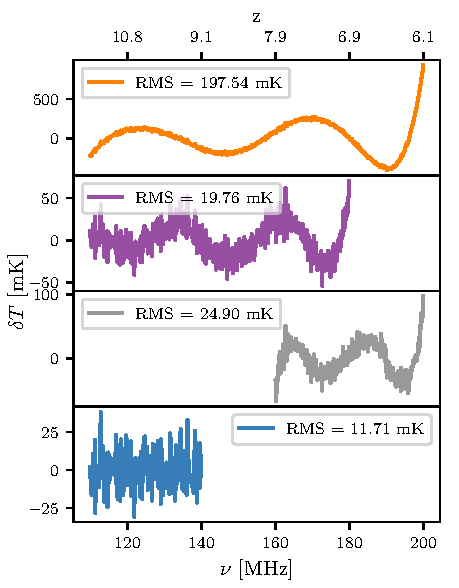
\includegraphics{saras2/figs/bandwidth.pdf}
    \caption{A comparison of the residuals when fitting the SARAS2 data with a $10^{th}$ order Partially Smooth Function with derivatives of order $m \geqslant 3$ constrained across the full SARAS2 band (orange) and a set of reduced bandwidths. We achieve a significantly lower RMS in the reduced bandwidths. This indicates either a poor foreground fit across the full bandwidth, which can introduce non-smooth structure, or the presence of multiple non-smooth systematics dominant at different frequencies. We proceed to perform our analysis in the reduced bandwidth 110-180 MHz based on the results presented in previous work \protect\citep{Singh_saras2_2017,SARAS2_radiometer_2018} and in order to retain as much data as possible.}
    \label{fig:foreground_res}
\end{figure}

\cref{fig:foreground_res} shows the resultant residuals, in orange, when fitting the data with the PSF model across the whole SARAS2 bandwidth. The residuals are large in magnitude and show a sinusoidal structure, which may be the result of systematics in the data and/or of inaccurate foreground modelling. 

In the previous analysis of the SARAS2 data, in which parameter constraints were determined from a discrete set of signal models, the bandwidth used was optimised on a per-signal basis \citep{Singh_saras2_2017, Singh_saras2_2018}. In that work, it was frequently found that the bandwidth $110-180$ MHz is the optimum to minimise the signal-to-noise ratio for the 264 tested signal models

In this work, the turning point and inflection point may be significantly distorting the foreground model leading to the introduction of spurious non-smooth structure in the residuals\footnote{This is unlikely, and it can actually be shown that Partially Smooth Functions can be effectively used to recover the noise in data sets that feature inflection points (see `Turning Points and Inflection Points' in \url{https://maxsmooth.readthedocs.io/en/latest/maxsmooth.html}).}, despite allowing for their presence in the modelling, and so we attempt to fit with a PSF in the reduced range $\nu = 110 - 180$ MHz effectively removing the turning point. We achieve significantly smaller residuals when fitting in this band, as shown in purple in \cref{fig:foreground_res}. The difference in magnitude may suggest a better quality foreground fit, but it may also indicate the presence of multiple non-smooth systematics in the data, each of which may dominate to a different degree at different frequencies. 

A further reduction in the upper bound on the frequency range leads to a further reduction in the RMS. However, we still see the same sinusoidal structure at low frequencies. In practice, we could reduce the band to 110 - 140 MHz, removing both the turning point and inflection point, and we would see a significantly lower RMS ($\approx 12$ mK when fitting with the proposed PSF model as can be seen in the bottom panel of \cref{fig:foreground_res}). This is because the systematic structure in the data in this frequency range covers one period of oscillation and is therefore smooth to a sufficient level that it is removed by the foreground model. Further, if we remove the inflection point in the data and fit in the range $160 - 200$ MHz we see a sinusoidal structure that is partially consistent with the purple residuals in \cref{fig:foreground_res}.

Throughout the rest of the chapter, in accordance with the previous SARAS2 analysis, to simplify the modelling and to keep as much data as possible, we use the reduced bandwidth $110 - 180$ MHz. The modelling of the non-smooth systematic structure is considered in the following section.

%We note that contributions from foreground polarization can generally be expected in the data. Modelling of the effects of polarization is non-trivial, however, and the intensity of corresponding contributions is dependent on a number of factors \citep{Spinelli_polarization_2018}. In \cite{Spinelli_polarization_2019} the authors show that contributions from polarisation have significant non-smooth structure and we would expect that, if this was present and dominant in our data, it would be obvious after modelling the foreground with a PSF. However, this is not the case in our residuals. Further, to a first approximation we expect that the polarized signal will be proportional to $1/\nu^2$ \citep{Spinelli_polarization_2018} and larger at lower frequencies following the opposite trend to our residuals. Therefore, any contribution from foreground polarization in our data can be considered sub-dominant and subsumed in our noise modelling.

In comparison to the predicted maximum depth of the global 21-cm signal \citep[$\approx 165$ mK for standard astrophysical signals in the band $110 - 180$ MHz,][]{Reis_sta_2021}, the residual RMS, $19.8$ mK, appears small in magnitude. However, as highlighted above and in \cite{Singh_saras2_2017} and \cite{Singh_saras2_2018}, any signal in the data will be suppressed by the total efficiency of the antenna. This is discussed further in \cref{sec:signal_modelling}. 

\subsection{Systematic Modelling}
\label{sec:systematic modelling}

\begin{figure}
    \centering
    \includegraphics[width=\linewidth]{saras2/figs/SARASRadiometerDiagram.pdf}
    \caption{A simplified schematic of a global 21-cm experiment. The figure illustrates the two positions at which systematic power could be added into $T_\mathrm{A}$; (A) prior to the antenna and (B) after the antenna in the receiver electronics, denoted by the time dependent gain, $G_\mathrm{RX}(t, \nu)$. Note, when modelling the systematic in the SARAS2 data, we are considering these scenarios independently. The former systematic arrives with the signal from the sky, $T_\mathrm{sky}(t, \nu, \Omega)$, and global signal, $T_{21}(\nu)$ if present, and passes through the antenna where it is weighted by the beam directivity, $D(\nu, \Omega)$. The angular dependence is integrated out, and the systematic is then multiplied by the total efficiency of the antenna, $\eta_t(\nu)$, giving $T_\mathrm{NS,2}$ as detailed in \cref{sec:systematic modelling}. The systematic introduced in the electronics corresponds to $T_\mathrm{NS,1}$ in \cref{sec:systematic modelling}. After passing through the electronics, the time dependence is also integrated out of the data leaving $T_A$. Figure modified from Fig.2 of \protect\cite{Cumner_antenna_2021}.}
    \label{fig:radiometer}
\end{figure}

Previous analysis has shown the potential presence of sinusoidal and damped sinusoidal systematics in data from several global 21-cm experiments using a variety of different radiometers and analysis techniques. One such example, previously mentioned in the introduction, is the EDGES data. In \cite{Hills2018} the authors used a foreground model with spectral index characterised by a 6 term unconstrained polynomial to identify a 60 mK sinusoidal structure in the EDGES data. A subsequent re-analysis of the data in \cite{Singh_edges_2019} and \cref{ch:maxsmooth} \cite{Bevins_maxsmooth_2021}, using MSFs to model the foregrounds, identified a similar sinusoidal structure. In \cref{ch:maxsmooth} we also re-analysed data from LEDA and identified the presence of a damped sinusoidal systematic structure using MSFs \cite{Bevins_maxsmooth_2021}. Previous investigation of the LEDA data in \cite{Price_LEDA_2018}, where the authors used a log-polynomial foreground model, also found sinusoidal structures.

Currently, systematics and the ambiguity of their causes pose a limiting factor in the detection and/or confidence of a detection in global 21-cm experiments. We attempt to physically motivate our model for the systematic structure in the SARAS2 data and, as a consequence of detailed systematic modelling, derive astrophysical parameter constraints on the global signal.

Specifically, we model the damped sinusoidal structure seen in the residuals after foreground subtraction with two different physically motivated systematic models representing the introduction of power at different points, (A) and (B), in the SARAS2 system as illustrated in \cref{fig:radiometer}. Any non-smooth systematic model can be included in \cref{eq:components} as an additive term
\begin{equation}
    T_\mathrm{A} = (T_{21} + T_\mathrm{fg})\eta_t + T_\mathrm{NS}.
    \label{eq:components_with_sys}
\end{equation}
The sinusoidal structure may be introduced by a poor estimate of $\eta_t$. However, when fitting the total efficiency with a best fitting MSF of the form given in \cref{eq:psf_fore} we find no sinusoidal structure in the residuals.
We also reiterate, for completeness, that the systematic structure may be being introduced by poor foreground modelling.

The first systematic model we use, which we refer to as the damped systematic model, corresponds to power introduced after the antenna and in the electronics \citep[e.g. see Fig. 2 in ][]{SARAS2_radiometer_2018}
\begin{equation}
    T_\mathrm{NS, 1}(\nu) = \bigg(\frac{\nu}{\nu_0}\bigg)^{\alpha_\mathrm{sys}} A \sin\bigg(\frac{2\pi\nu}{P} + \phi\bigg),
    \label{eq:damped_sys}
\end{equation}
where $\alpha_\mathrm{sys}$ is a damping power, $A$ is the amplitude of the systematic, $P$ is the period, $\phi$ is the phase and $\nu_0$ is the central frequency in the band. We note that the prior range of $\alpha_\mathrm{sys}$ ranges from $0 - 10$ (see \cref{tab:priors} for all the systematic prior ranges) and as a result the model can also account for sinusoidal systematics. %The fitted parameters, $A$, $\alpha_\mathrm{sys}$, $P$ and $\phi$ are constant across the band and the frequency dependence comes from the damping factor, $(\nu/\nu_0)^{\alpha_\mathrm{sys}}$.

The second model, referred to as the efficiency systematic, is given by
\begin{equation}
    T_\mathrm{NS, 2}(\nu) = \eta_t \bigg(\frac{\nu}{\nu_0}\bigg)^{\alpha_\mathrm{sys}} A \sin\bigg(\frac{2\pi\nu}{P} + \phi\bigg).
    \label{eq:eff_sys}
\end{equation}
In this case, the systematic structure models power introduced prior to the antenna and mediated by the total efficiency which introduces some damping. Such a systematic could be explained by activity in the ionosphere over the observing period, RFI or a previously unidentified non-smooth component of the foreground.

The non-smooth structure in the data could also, as highlighted previously, be caused by emission from the ground if the assumption that this is smooth does not hold. Specifically, structure or layering in the ground at depths larger than the wavelengths of operation and below the penetration depth computed for the soil properties could introduce systematic structure. A discontinuity in the soil below the antenna such as that between the loose topsoil, caused by erosion over time, and the rock of the Deccan Plateau or from a water table could cause a damped sinusoidal structure to propagate through to the receiver noise, total efficiency and antenna temperature.

Another possible origin of a damped sinusoidal systematic could be a small clump of foliage or a root system, without significant foliage above ground, close to the deployment site. In principle, both this and ground emission are potential causes of systematics that will be mitigated in the latest iteration of the SARAS experiment, SARAS3, which has been deployed on a lake \citep{SARAS3_spectrometer_2020, SARAS_reciever_2021, SARAS3_antenna_2021}.

It is well-known that the directivity of vertical monopoles ~\citep{5492282} naturally experiences a sinusoidal like frequency response. Such behaviour would correspond to $T_\mathrm{NS, 2}$. We note, however, that the period of the sinusoidal-like structure visible in the data is faster than what would be expected from a monopole. The scale of the circular element of the antenna, 43.5 cm in radius, was chosen such that any reflections from the edges of the disks would have a period of $\approx 350$ MHz and the observing band falls within the first resonance at $260$ MHz \citep{Singh_saras2_2017, SARAS2_radiometer_2018}. Any reflections in the beam pattern from the edges of the disk would thus be smooth across the reduced SARAS2 band and effectively subsumed by our smooth foreground model detailed in the previous subsection.

If we consider the systematic to be real and not a spurious signal introduced by an inaccurate foreground model, then our analysis could help to identify the point at which the power is introduced into the system. We note that there may be degeneracy between the two different models, but also that the efficiency is an inherent characteristic of the experiment and unlikely to mimic generic systematic properties.

\begin{table}
    \centering
    \begin{tabular}{|P{1.5cm}|P{1.5cm}|P{5cm}|P{2cm}|}
        \hline
         & Parameter & Prior & Prior Type\\
        \hline
        \hline
        \multirow{4}{*}{Systematic}& $\alpha_\mathrm{sys}$ & $0 - 10$ & \multirow{4}{*}{Uniform}\\
        & $A$ & $0 - 1$ K  & \\
        & $P$ & $10 - 70$ MHz &  \\
        & $\phi$ & $0 - 2\pi$ rad & \\
        \hline
        \hline
        \multirow{8}{*}{Signal}& $\tau$  & $0.026 - 0.1$ (STA) / $0.035 - 0.077$ (ERB) & \multirow{4}{*}{Uniform}\\
        & $\alpha$ & 1.3 (STA only) & \\
        & $E_\mathrm{min}$ & $0.1 - 3$ keV (STA only) &\\
        & $R_\mathrm{mfp}$ & 30 (STA) / 40 (ERB) Mpc &\\
        \cline{2-4}
        & $f_*$ & $0.001 - 0.5$ &  \multirow{4}{*}{Log-Uniform}\\
        & $V_c$ & $4.2 - 100$ km/s & \\
        & $f_X$ & $0.0001 - 1000$ & \\ 
        &$f_\mathrm{radio}$ & $1 - 99500$ (ERB only) & \\
        \hline
    \end{tabular}
    \caption{The prior ranges and prior types used for the systematic and signal parameters fitted by \textsc{polychord}. Note that for the signal parameters, the prior ranges are defined by the neural network training data. For the excess radio background (ERB) signals $R_\mathrm{rmfp}$ is fixed at 40 Mpc and the X-ray SED is representative of that from X-ray binaries\cite{Fragos_Xrays_2013}. See \cref{sec:signal_modelling} for more details on each model component, the training data and the difference between the standard astrophysical (STA) and ERB models.}
    \label{tab:priors}
\end{table}

\subsection{Signal Modelling}
\label{sec:signal_modelling}

%The signal emulator \textsc{globalemu} provides a framework to train neural networks on different sets of global 21-cm signals. We can therefore use the latest simulations with the most up-to-date understanding of the signal, and we can analyse parameter constraints on different astrophysical models. 

To recap, the global 21-cm signal is determined by the contrast between the spin temperature of neutral hydrogen, $T_s$, and the radio background, $T_r$, as a function of redshift
\begin{equation}
    T_{21} = \frac{T_s -T_r}{1+z}(1 - e^{-\tau_{21}}),
    \label{eq:deltaT}
\end{equation}
where $\tau_{21}$ is the 21-cm optical depth of the IGM \citep{Mesinger2019}. Calculated realisations of the global 21-cm signal are achieved by using hybrid techniques and either averaging over large modelled cosmological volumes \citep[2D simulations e.g.][]{Mesinger2011} or directly approximating that average over redshift \citep[1D simulations e.g.][]{ARES_sim}. In this analysis we use the simulations detailed in \cite{Visbal_2012, Fialkov_rich_2014, Cohen_global_2017, Reis2020, Reis_sta_2021} and specifically the sets of global 21-cm signals presented in \cite{Reis2020} and \cite{Reis_sta_2021}. For each set of signals, exotic models with an excess radio background and standard astrophysics respectively, we train neural network emulators with \textsc{globalemu}. More details about the two sets of signal models we have used are given in the following sections, with examples shown in \cref{fig:signals}.

%\begin{landscape}
\begin{figure*}
    \centering
    \includegraphics{saras2/figs/signals.pdf}
    \caption{\textbf{Top Row, left to right:} A set of 50 example signals that include Lyman-$\alpha$ heating and CMB heating, the equivalent signals in the band $110 - 180$ MHz and the signals multiplied by the total efficiency of the SARAS2 antenna. \textbf{Bottom Row, left to right:} 50 example signals with different levels of excess radio background above the CMB, the same signals in the reduced SARAS2 band and finally the signals multiplied by the total efficiency of the SARAS2 antenna.}
    \label{fig:signals}
\end{figure*}
%\end{landscape}

\subsubsection{Standard astrophysical signals}

In this chapter, we use the recent simulations of the global signal with Lyman-$\alpha$ heating, CMB heating and multiple scattering presented in \cite{Reis_sta_2021}. We refer to these standard astrophysical models in the text as the STA (standard astrophysical) signals. %As stars form in the early universe and Lyman-$\alpha$ coupling between the spin temperature, $T_s$, of the neutral hydrogen and kinetic temperature of the gas, $T_k$, begins to influence the structure of global signal, Lyman-$\alpha$ and CMB heating begin to counteract the cooling \citep[][]{Chuzhoy2007, Venumadhav2018, Mittal2021, Reis_sta_2021}. These heating mechanisms begin before the onset of X-ray heating and they lead to a reduction in the theoretical maximum potential depth of absorption from $\approx250$ mK \citep{Cohen2020} to $\approx 165$ mK \citep{Reis_sta_2021}. 
We note that, multiple scattering primarily influences the structure of the power spectrum at $z > 20$ \citep{Reis_sta_2021} outside the SARAS2 band.

We train \textsc{globalemu} on a set of 5,137 realisations of the standard astrophysical signals and test the quality of emulation with a set of 570 models. Each model spans the redshift range $z = 6 - 39$ and the redshift spacing is given by $\delta z = 0.1$. The structure of the signals is determined by a set of seven astrophysical parameters \citep[further details can be found in the introduction of the thesis and ][]{Cohen2020, Reis_sta_2021, Bevins_globalemu_2021};

\begin{itemize}
    \item The star formation efficiency, $f_*$: Determines the fraction of gas in dark matter halos that is converted into stars. The value of $f_*$ drives the Lyman-$\alpha$ flux and influences the onset of X-ray heating, which both determine the depth of the global signal absorption trough and the ionizing efficiency of sources.
    \item The minimal circular velocity, $V_c$: The threshold virial circular velocity is proportional to the cube root of the minimum halo mass for star formation. Its value is determined by different
    cooling channels (molecular and atomic hydrogen) and star-formation-suppressing feedback mechanisms. It influences the timing of Lyman-$\alpha$ coupling, total X-ray luminosity of halos and reionization.
    \item The X-ray efficiency, $f_X$: The value of $f_X$ affects the X-ray luminosity per star formation rate, which in turn influences the depth of the absorption trough and amplitude of any emission above the radio background during reionization. $f_X$ also has a minor effect on reionization.
    \item The slope of the X-ray spectral energy distribution~(SED), $\alpha$: The dependence of the structure of the global signal on $\alpha$ is expected to be very weak \citep{Monsalve_EDGES_HB_3_2019} and its value plays a small role at low redshifts.
    \item The low energy cut-off of the X-ray SED, $E_\mathrm{min}$: This parameter has some influence on the efficiency of X-ray heating at low redshifts covered by the SARAS2 band. While it is not expected to affect the structure of the signal significantly, in some cases, it can have more of an impact than $\alpha$ or $R_\mathrm{mfp}$.
    \item CMB optical depth, $\tau$: The optical depth is directly related to the ionizing efficiency of sources, $\zeta$ and its value strongly influences the redshift of reionization. The value of $\tau$ has been determined by \cite{Planck2018} to be $0.055 \pm 0.007$ and \cref{tab:priors} shows that this range is explored completely by the prior for the STA models.
    \item The mean free path of ionizing photons, $R_\mathrm{mfp}$: The value of $R_\mathrm{mfp}$ affects the rate of ionization of the neutral hydrogen gas corresponding to the gradient of the signal at low redshifts. The effects of varying $R_\mathrm{mfp}$ are also not expected to influence the structure of the global signal significantly \citep[see e.g. ][]{Monsalve_EDGES_HB_3_2019}.
\end{itemize}

The primary reason $E_\mathrm{min}$, $\alpha$ and $R_\mathrm{mfp}$, are explored in the simulations is because the simulations are also used to determine models of the power spectrum on which they have a greater influence. We train \textsc{globalemu} using all seven astrophysical parameters and subsequently perform fits with fixed values of $R_\mathrm{mfp} = 30$ Mpc and $\alpha = 1.3$ \citep[as was done with the EDGES High Band data in ][ using the contemporary standard astrophysical models and signal emulator]{Monsalve_EDGES_HB_3_2019}. We repeat the analysis in Appendix D of \cite{Bevins_SARAS2_2022} allowing \textsc{polychord} to fit for all seven parameters, however we do not discuss these results in the main text as we find the effect of including the additional parameters is minimal. The ranges, equivalent to the priors, of all the parameters sampled in the training and test data sets are given in \cref{tab:priors}.

We assess the accuracy of the emulator across the band $110 - 180$ MHz (or equivalently $z \approx 7 - 12$). We use a pragmatic target accuracy when emulating the signals of on average approximately 10\% of the expected noise from a global 21-cm experiment \citep{Bevins_globalemu_2021}. This varies based on the experiment with a value of 2.5 mK for REACH, 2 mK for EDGES \citep{Bowman_edges_2018} and approximately 1 mK for SARAS2. Therefore, when emulating the STA models, we assume a target accuracy of between 1 and 2.5 mK and use the RMSE metric given by equation (7) in \cite{Bevins_globalemu_2021}. The mean, 95$\textsuperscript{th}$ percentile and the worst RMSE values from the test data set of 570 models, with sampling resolution equivalent to 0.122 MHz, are 0.8, 1.9 and 6.8 mK respectively. We find that only 29 models have an RMSE larger than $\approx 1.9$ mK indicating a high degree of accuracy. We use a fully connected network with 4 hidden layers of 16 nodes each to emulate the STA models.

%In practice, a low RMSE in temperature does not necessarily correspond to an accurate recovery of the astrophysical parameters. For the analysis performed in this work, this is not a significant issue because the reported constraints are weak. We leave a detailed exploration of emulator accuracy and its effects on parameter recovery for future work.

\subsubsection{Excess radio background signals}

Typically, $T_r$ in \cref{eq:deltaT} is assumed to be equal to the CMB temperature. However, as discussed in \cref{ch:introduction}, one of the possible explanations for the larger than expected absorption feature reported by EDGES \citep{Bowman_edges_2018} is an excess radio background above the CMB. In addition, a population of radio sources at high redshifts could naturally contribute to $T_r$ \citep[e.g][]{FengRB2018}. While there is some evidence for a larger than expected radio background from ARCADE2 \citep{fixsen_arcade_2011} and LWA \citep{dowell_radio_2018}, there remain some concerns about the Galactic modelling in these works \citep{Subrahmanyan2013}.

\cite{Reis2020} investigated the introduction of an excess radio background from high redshift radio galaxies, and we use the models presented there in this work in an attempt to constrain the parameter $f_\mathrm{radio}$ with the SARAS2 data. $f_\mathrm{radio}$ denotes the radio production efficiency of early galaxies, a value of one corresponds to the present day and the range of $f_\mathrm{radio}$ in our training data set is given in \cref{tab:priors}. We refer to these exotic astrophysical models throughout the rest of the chapter as the ERB (excess radio background) models.

The simulations use a similar parameter description of the global signal presented in the previous subsection with the additional parameter $f_\mathrm{radio}$. The value of $R_\mathrm{mfp}$ is fixed at $40$~Mpc when running the simulations. The X-ray SED is assumed to be from X-ray binaries \citep{fialkov_observable_2014}, and the simulations are consequently independent of $\alpha$ and $E_\mathrm{min}$. The models also include the effects of Lyman-$\alpha$ heating, CMB heating and multiple scattering. 

The data set contains 4,311 training models and 479 test models. We train \textsc{globalemu} with the five parameters as inputs; $f_*$, $V_c$, $f_X$, $\tau$ and $f_\mathrm{radio}$. The mean, 95th percentile and the worst RMSE values are 7.3, 27.3 and 125.9 mK respectively. We use a network with 4 hidden layers each with 16 nodes as was done with the STA models and note that with this training data set the accuracy does not significantly improve if we increase the size of the network. However, the mean accuracy of emulation, $7.3$ mK, is the same order of magnitude as our target accuracy of $1 - 2.5$ mK. The magnitudes of the signals with the largest errors, after multiplication by $\eta_t$, are significant in comparison to the expected noise and as fractional accuracies the worst and 95th percentile results are reasonable.

\section{Sensitivity of the SARAS2 Data to Astrophysical Parameters}
\label{sec:sensitivity}

When considering the sensitivity of the SARAS2 data to the global 21-cm signal, it is important to consider that any signal in the data will be multiplied by the total efficiency of the antenna. As has previously been discussed and shown in \cref{fig:signals}, this significantly reduces the magnitude of the signals in the data and given the expected noise of $11$ mK results in a low signal-to-noise ratio. In turn, this makes any signal in the data hard to recover.

Further, the observations cover a bandwidth expected to include the EoR which has implications for the types of signals that we expect to be able to constrain. The EoR window is sensitive to the value of $\tau$ which affects the redshift of reionization and as a result the maximum amplitude of the global signal. For example, a high value of $\tau$ can lead to an earlier reionization. However, in the absence of efficient X-ray heating and presence of a low Lyman-$\alpha$ flux the effect of $\tau$ is less significant in the SARAS2 bandwidth.

Similarly, the value of $E_\mathrm{min}$ has a more significant effect on the structure of the global signal in the SARAS2 band if $f_X$ is high. In this case, the value of $E_\mathrm{min}$ affects the depth of the signal and the efficiency of X-ray heating. If we maintain the Lyman-$\alpha$ flux, i.e. onset of Lyman-$\alpha$ coupling, and increase the value of $E_\mathrm{min}$ we reduce the efficiency of X-ray heating, move the minimum of the signal to lower redshifts and can create a deep global signal inside the SARAS2 band. A similar effect can occur if we decrease the value of $f_X$ from high to low, and this is more prominent than that introduced by variation in $E_\mathrm{min}$. The analysis should therefore be sensitive to models with low values of $f_X$ and high values of $E_\mathrm{min}$.

In addition, if $f_X$ is high, and to a lesser extent if $E_\mathrm{min}$ is low, then we can expect that there will be significant excess radio background which will produce a prominent and deep signal in the SARAS2 data even after multiplication by the total efficiency of the antenna.

$V_c$ and $f_*$ determine the strength of the Lyman-$\alpha$ flux, consequent onset of Lyman-$\alpha$ coupling and position of the signal minimum. High values of $f_*$ correspond to a high fraction of the gas in dark matter halos being converted into stars, which leads to a high Lyman-$\alpha$ flux. The top panels of \cref{fig:sensitivity} show that the strongest signals in the SARAS2 band after multiplication by the total efficiency are those with low Lyman-$\alpha$ fluxes (high $V_c$ and low $f_*$) whereas the weakest signals are those with high Lyman-$\alpha$ fluxes (low $V_c$ and high $f_*$). Here, we have defined ``high'' and ``low'' values of the parameters with respect to the middle of the log-prior ranges. Our analysis should therefore be more sensitive to models with low Lyman-$\alpha$ fluxes.

Further, dividing the two classes of signals in \cref{fig:sensitivity} based on their value of $f_X$ we can see that we should also expect our analysis to be sensitive to low values of $f_X$, as expected from the discussion above.

We should also consider our sensitivity to models that have both high or both low values of $V_c$ and $f_*$ in combinations that do not meet the crude criteria for high and low Lyman-$\alpha$ fluxes defined above. These models are shown in black in the bottom panel of \cref{fig:sensitivity} against the backdrop of previously ``classified'' models in grey. From the figure we can see that these models typically also have low Lyman-$\alpha$ fluxes and have minima at more recent redshifts, particularly in comparison to the ``high'' Lyman-$\alpha$ flux signals discussed previously. These signals therefore have dominant structures and relatively large magnitudes in the SARAS2 band, and indicate a more general sensitivity to the values of $f_*$ and $V_c$.

Finally, the data is expected to be sensitive to ERB signals with very high values of $f_\mathrm{radio}$ as these signals have deep absorption troughs of a few hundred mK even after multiplication by the total efficiency of the antenna. This is particularly true when there is also a high Lyman-$\alpha$ flux and low X-ray efficiency, which results in strong variation of the signal within the SARAS2 band.

\begin{figure*}
    \centering
    \includegraphics{saras2/figs/sensitivity.pdf}
    \caption{The figure shows 243 STA signals from the testing data coloured based on the values of $f_*$, $V_c$ and $f_X$. The left column shows the signals as they are in the testing data and the right panel shows the signals in the SARAS2 band, indicated on the left by the dashed lines, after multiplication by the total efficiency of the antenna. In the top panels, we show the set of signals split based on the type of Lyman-$\alpha$ flux that they correspond to. A high Lyman-$\alpha$ flux is produced by a high $f_*$ and low $V_c$ where we judge `low' and `high' with respect to the middle of the log-prior range for each parameter. In the middle panels, we further split the models based on their values of $f_X$. From the graph we can see that, after multiplying by the total efficiency of the SARAS2 antenna, the signals with a low Lyman-$\alpha$ flux and low value of $f_X$ have the largest absolute magnitudes and so our analysis should be most sensitive to these models. The bottom panel shows the previously classified 243 STA signals in grey in comparison to a further 257 signals in black that do not meet our crude classification of `low' and `high' Lyman-$\alpha$ fluxes and with neither high $f_*$ and low $V_c$ or low $f_*$ and high $V_c$. These models have prominent structures in the SARAS2 band, indicating a more general sensitivity to the values of $f_*$ and $V_c$.}
    \label{fig:sensitivity}
\end{figure*}

\section{Results}
\label{sec:results_saras2}

\Cref{fig:model_fits_graph} summarises the different combinations of signal, systematic and noise models that were fitted to the SARAS2 data. For completeness, we report fits without signals and/or systematics. The four fits with the highest Bayesian evidence are approximately equivalent (within error bars) and the relative weights based noise model is comparatively poor compared to the two alternatives considered when we include a systematic model in the fit. These points are further discussed in the following sections.

The evidence, $Z$, is a marginal likelihood integrated overall the fitted parameters. It quantifies the probability that the data is described by the chosen model components and is the normalising factor in Bayes theorem. A higher $\log(Z)$ indicates a preference for that model or hypothesis as a description of the data. %It is often used to determine the presence or absence of signals in data sets by comparing its value for fits with and without the relevant model components. An example of this, beyond the results presented in this chapter, can be found earlier in this thesis in \cref{ch:maxsmooth} where we fitted the EDGES data set with signal and systematic models using the evidence to determine which models are preferred by the data. A further brief discussion of the evidence and Bayes theorem can be found in Appendix A in \cite{Bevins_SARAS2_2022}.

\begin{figure*}
    \centering
    \includegraphics{saras2/figs/extended_table6_plot_fra_only_big_graph.pdf}
    \caption{A graphical summary of the different fits performed in this analysis, which demonstrates that the highest evidence fits from all of those performed are fits of equal quality. The signal type can be found on the right-hand y-axis, the fit number on the left-hand axis and the noise and systematic types in the legends. The fit numbers are used for referencing throughout the text. The top panel shows fits that include a systematic model, and the bottom panel shows fits without a systematic model. We divide the two classes of fits into separate graphs because those with a systematic have a much higher evidence, $\Delta \log(Z) \approx 200-300$, than those without. Note that a difference of $\Delta \log(Z) \approx 10$ corresponds to a difference of $\exp(10)\approx 22000$ or betting odds of 22000:1 in favour of the higher evidence model.}
    \label{fig:model_fits_graph}
\end{figure*}

Of the tested combinations of model components we find that modelling with a STA signal and no systematic leads to only a marginal increase in evidence in comparison to a foreground only fit as can be seen in the bottom panel of \cref{fig:model_fits_graph}. The increase in evidence is larger when we model an ERB signal and no systematic, but this is to be expected as these signals can have significantly deeper absorption features than the STA signals and as a result they are better able to fit out the larger systematic structure. Fits with systematic modelling have significantly higher evidences, regardless of whether we include an STA, ERB or no global signal model, than those without systematic modelling, $\Delta \log(Z) \approx 200 - 300$. The data, therefore, favours the presence of a systematic model, but there is no strong indication for the presence of a signal in the data. 

Appendix B in \cite{Bevins_SARAS2_2022} shows the residuals found when fitting the data with the PSF foreground model, no signal model, the efficiency systematic and the constant noise model~(fit number 4) compared with the residuals from a high order polynomial fit. The consistency between the two sets of residuals suggests that the complexity of the modelling used here is sufficient to describe the data. Although, a signal may still be present with an absolute maximum magnitude less than the noise after multiplication by the total efficiency of the antenna.

In the following sections, we discuss in more detail the results found when modelling with the different components outlined in \cref{sec:modelling}.

\subsection{Noise}
\label{sec:noise_results}

\begin{figure}
    \centering
    \includegraphics{saras2/figs/noise_models_posteriors.pdf}
    \caption{The posteriors for the noise parameters when fitting the SARAS2 data with STA signals and the efficiency systematic. The posteriors for the amplitude of the noise are near identical for the frequency damped (purple) and constant noise models (orange). In addition, $\beta_\sigma \approx0.5$ which corresponds to very weak damping. In combination, these two facts indicate a similarity between the two noise models. All the corner plots presented in this chapter were produced using \textsc{anesthetic} \citep{anesthetic} and the contour lines here represent 68\% and 95\% confidence intervals.}
    \label{fig:noise_posterior_example}
\end{figure}

We would expect that the relative weights based noise model would provide the best representation of the noise in the data as it has been derived from system parameters. In the absence of systematic modelling, this noise model performs comparatively well because the residuals after foreground modelling are larger at higher frequencies, following the trend of the weights. However, from the top panel of \cref{fig:model_fits_graph} it is clear that the log-evidence for fits with this noise model and a systematic is much lower than for fits with the two alternatives. This is likely due to some degeneracy, that would be hard to disentangle, between the systematic model and the weights based noise model which follow the same trend in the data (increasing with frequency). %However, the systematic model, particularly the damped systematic, is designed to allow for no damping (i.e $\alpha_\mathrm{sys} = 0$ in \cref{eq:eff_sys} and \cref{eq:damped_sys}) and we find that some damping is typically favoured in our fits as is the presence of a systematic model.

For some combinations of signal and systematic, we find that the log-evidence is comparable between the fits with constant and frequency damped standard deviation. However, in the majority of cases, the constant noise modelling gives a higher evidence. In the one case where this is not true, fitting with a STA signal and the efficiency systematic, the evidences are comparable, indicating that neither noise model is favoured over the other.

For the fit with the efficiency systematic and STA signals, we find, with the frequency damped noise, $\log(Z) = 1684.5 \pm 0.2$. In comparison, when modelling the noise with a constant standard deviation, we find $\log(Z) = 1684.4 \pm 0.2$. For these two fits, we can look in more detail at the maximum likelihood noise models, and the posteriors for the noise model parameters are shown in \cref{fig:noise_posterior_example}. For the frequency damped model the maximum likelihood parameters are $A_\sigma = 10.9$ mK and $\beta_\sigma = 0.45$ and for the constant noise model the maximum likelihood amplitude is $A_\sigma = 11.0$ mK. In the former, the damping power is weak, recalling that the prior range for this parameter is $0 - 5$, and the maximum likelihood amplitude for both models is near identical with a similar posterior distribution. The weak damping is a consistent feature across all the fits with the damped model, as is the similarity in the amplitude of the noise.

To summarise, when comparing the two best noise models, constant and frequency damped, we find an equality in log-evidence or preference for the former model, a consistent weak damping in the latter and similarity in amplitude. This supports the expectation from the literature that the noise should be uniform across the band in the SARAS2 data \citep{Singh_saras2_2017,Singh_saras2_2018}.

\subsection{Systematics}

As discussed, we see a large increase in log-evidence, $\Delta~\log(Z)~\approx 300$, when joint fits with a PSF foreground and the efficiency or damped systematic models are performed as shown in \cref{fig:model_fits_graph}. Comparing like for like fits with different systematic models, we consistently find that the efficiency systematic model is favoured over the alternative by the data. Regardless of noise modelling, the five highest evidence models are all fits with the efficiency systematic.

Both systematics rely on the same parameterisation and so a direct comparison can be made between fits with the same noise and signal modelling but different systematic models. The posterior distributions for each parameter are typically well constrained Gaussian-like distributions. $\alpha_\mathrm{sys}$ is generally centred around 0 for the efficiency systematic, in comparison to a value of approximately 3 for the damped systematic. This indicates that, in the case of the efficiency systematic, the data favours a sinusoidal systematic structure that is damped predominantly by the total efficiency of the radiometer, $\eta_t$ (i.e. the term $(\nu / \nu_0)^{\alpha_\mathrm{sys}} \approx 1$ in \cref{eq:eff_sys}).

For both systematic models the period, $P$, and phase, $\phi$, have similar distributions, suggesting that any systematic in the data has a period of $\approx32.5$ MHz and phase of $\approx0$ rad. This is true generally, regardless of noise and signal model, since the systematic dominates the residuals. The systematics also have similar amplitudes but, while in the efficiency systematic this is mainly determined by $A$, in the damped systematic it is mainly determined by the term $(\nu / \nu_0)^{\alpha_\mathrm{sys}}$ in \cref{eq:damped_sys}.

From the log-evidences, we can conclude that the data marginally favours a sinusoidal systematic damped by the total efficiency of the antenna. However, as with the noise modelling, the differences in log-evidence between like for like fits with different systematics are small and all the fits with the different systematic models contain potential information about the astrophysical parameter space. We can, therefore, use all the samples from the different fits, weighted by their evidences, in a combined analysis. This approach effectively marginalises over the systematic and noise model parameters and is detailed in the following section.

\subsection{Disfavoured 21-cm signals from combined samples}
\label{sec:disfavoured_regions_combined_samples}

We can use \textsc{anesthetic} \citep{anesthetic} to combine the posterior samples from \textsc{polychord}, weighted by the fit evidence, from the various Nested Sampling runs to determine the types of global 21-cm signals disfavoured in our analysis. This is advantageous since it provides a method to deal with uncertainty in the modelling of the standard deviation on the noise and the systematic, and should be considered a conservative view of any constraints on the parameter space from the SARAS2 data.

While we note that the fits in \cref{fig:model_fits_graph} do not indicate a preference for the presence of a signal, we can still use the data to determine constraints on the parameter space of the global 21-cm signal, as has previously been done with data from EDGES \citep{Monsalve_EDGES_HB_3_2019}.

In the previous two sections we have made the argument that the amplitude of the noise is best described by a constant standard deviation and the systematic is best modelled by the efficiency systematic. While these statements are true to an extent, the range in log-evidence between the corresponding fits with different model components is not significant. In fact, the former is largely motivated by the fact that the constant noise model is simpler than the frequency damped model and thus favourable. In practice, the data does not tell us which noise model is preferred.

Since the 2D and 1D posteriors for the astrophysical parameters, $\theta_{21}$, by definition marginalise over the systematic and noise parameters, we can confidently combine the samples and draw conclusions from the corresponding posteriors. As alluded to the posterior samples, $P(\theta|D, M)$, when combined using \textsc{anesthetic} are weighted by weights, $w$, that are directly proportional to the fit evidence, $Z$
\begin{equation}
    P_\mathrm{combined}(\theta_{21}|D, M) = \sum_i w_i P_i(\theta_{21}|D, M),
    \label{eq:combined_samples}
\end{equation}
where the weights $w_i = Z_i/\sum_j Z_j$, $\theta_{21}$ is a vector of astrophysical signal parameters for fit $i$, $D$ is the data and $M$ is the analytical model. In Appendix C in \cite{Bevins_SARAS2_2022} we show the values of $w_i$ for each of the different fits performed in this analysis separated by their signal type.

In the following subsections, we therefore discuss posteriors from combined samples for all the fits containing STA signals (see Appendix D in \cite{Bevins_SARAS2_2022} for results with variable values of $R_\mathrm{mfp}$ and $\alpha$) and fits containing ERB signals.

We briefly compare our results with those previously reported in \cite{Singh_saras2_2017, Singh_saras2_2018} and with results published in early 2022 from HERA \cite{HERA_2022b} in \cref{sec:comparison}.

\subsubsection{Excess Radio Background Signals}

We can analyse combined samples from fit numbers 1, 5, 10, 12, 14 and 16, those containing ERB signals, as shown in \cref{fig:combined_samples_fradio}. The recovered 1D histograms are generally flat and do not show any significant constraints. Although regions of high $f_\mathrm{radio}$ ($\gtrsim$ 407 and $\gtrsim$ 707)
in combination, separately, with low $f_X$ ($\lesssim$ 0.21) and high $f_*$ ($\gtrsim$ 0.03) are disfavoured at 68\% confidence. %We also disfavour high values of $\tau$ above approximately $\gtrsim$ 0.06 in combination with $f_X \gtrsim 0.50$ at 68\% confidence.

We use histograms to illustrate the samples in the parameter space. % rather than plotting posteriors, with confidence regions, derived using Kernel Density Estimation~(KDE) as was done in \cref{fig:noise_posterior_example}. This is done because the application of a KDE to the samples can, in the case of flat distributions, lead to misleading features that suggest specific areas of the parameter space are more favourable than others. 
Binning the raw samples across the parameter space gives a clearer impression of regions of the parameter space that the Nested Sampling algorithm explored in greater detail (i.e. those with higher likelihoods and combinations of parameters that are favoured by the data). For example, in \cref{fig:combined_samples_fradio} favoured regions of the parameter space would be sampled in greater detail and the corresponding bins in the 2D plots would be shaded in a lighter yellow.

To quantify the strength of 2D constraints across the parameter space, the authors of \cite{HERA_2022b} assess the ratio of the minimum and maximum posterior probability ($\propto$ height of the histogram bins) across the 2D space. A ratio of 1 would indicate a perfectly flat posterior, and a low value indicates a non-uniform distribution. The metric is limited in that it does not indicate the direction of any non-uniformity and is insensitive to any pseudo-random scatter across the parameter space that may result from a fine binning of a relatively flat distribution\footnote{The metric is also dependent on the number of bins into which the samples are separated and so comparison across experiments is difficult.}. However, in combination with a visual inspection of a constrained parameter space, it can be a useful metric to determine the magnitude of any directional non-uniformity. For example, the ratio between the minimum and maximum posterior probability for $f_\mathrm{radio}-f_X$ in \cref{fig:combined_samples_fradio} is 0.10. In comparison, the maximum ratio is 0.20 for $V_c - f_\mathrm{radio}$ and the minimum ratio is 0.08 for $f_X - \tau$.

\begin{figure*}
    \centering
    \includegraphics{saras2/figs/fradio_merged_samples_posterior_hist.pdf}
    \caption{The 1D and 2D distributions for the combined nested samples of all fits to the SARAS2 data containing ERB signals. The solid contours in the 2D parameter space enclose 68\% confidence regions, and the dashed contours enclose 95\% confidence regions. Combinations of high $f_*$ ($\gtrsim$ 0.03) and high $f_\mathrm{radio}$ ($\gtrsim$ 707) as well as low $f_X$ ($\lesssim$0.21) and high $f_\mathrm{radio}$ ($\gtrsim$ 407) are less densely sampled than the rest of the parameter space and are consequently disfavoured in our analysis.}
    \label{fig:combined_samples_fradio}
\end{figure*}

Further, the deepest signals have high Lyman-$\alpha$ fluxes (high $f_*$ and low $V_c$), low X-ray efficiencies, $f_X$, and high values of $f_\mathrm{radio}$. After multiplication by the total efficiency of the antenna these signals typically have magnitudes larger than the expected noise, and consequently we would expect to exclude these with the SARAS2 data. This can be seen clearly in \cref{fig:fradio_fgivenx} in which we plot the functional posterior samples in red on top of the prior in blue using the tool \textsc{fgivenx} \citep{fgivenx}. The tool allows us to visualize the combined posterior samples shown in \cref{fig:combined_samples_lyh_fra} as a set of contours in the $T_{21} - z$ space. Note that although the priors on our parameters are uniform, this does not necessarily translate to a uniform prior in the global 21-cm signal.

\begin{figure*}
    \centering
    \includegraphics{saras2/figs/fgivenx_signals_nlive_500_fradio_only.pdf}
    \caption{The figure shows the contraction from the prior (blue) to the combined posterior samples (red) in the 5D astrophysical parameter space (i.e. $T_{21} - z$) for the ERB signals. We plot the prior in blue and posterior in red on top of each other to highlight that we rule out the deepest of these exotic astrophysical models. The figure was produced using \textsc{fgivenx} \protect\citep{fgivenx}.}
    \label{fig:fradio_fgivenx}
\end{figure*}

\subsubsection{Standard Astrophysical Signals}

Histograms produced from the combined samples for the astrophysical parameters from fit numbers 2, 3, 9, 11, 13, and 18 from \cref{fig:model_fits_graph}, those with STA signals, are shown in \cref{fig:combined_samples_lyh_fra}. The histograms are flat, indicating that we do not significantly constrain the parameter space, and further indicating that there is no preference for a signal in the data.

\begin{figure*}
    \centering
    \includegraphics{saras2/figs/lyh_merged_samples_posterior_fixed_rmfp_alpha_hist.pdf}
    \caption{The 1D and 2D histogram plots from the combined nested samples of all fits to the SARAS2 data containing STA signals with fixed values of $R_\mathrm{mfp}$ and $\alpha$. The solid contours in the 2D posteriors enclose regions of 68\% confidence, and the dashed contours enclose regions of 95\% confidence.
    The histograms are relatively flat, and we do not disfavour values of individual parameters.}
    \label{fig:combined_samples_lyh_fra}
\end{figure*}


\cref{fig:fgivenx_lah} shows the functional posterior in red, along with the equivalent for samples taken from the prior in blue. There is some indication that the data disfavours (lighter shaded red regions) signals with absorption features at high redshift. For example, the preferred region (darker red and blue with significance $<1\sigma$) around the absorption minimum, where the sampling is highest, is larger and shifted to lower redshifts in the posterior than in the prior. However, the contraction from the prior to the posterior is minimal, as would be expected from the flat nature of the distributions in \cref{fig:combined_samples_lyh_fra}. Therefore, any conclusions we make about constraints on the standard astrophysical priors are by definition very weak. 

%The contraction from prior to posterior can be quantified with the Kullback-Leibler Divergence and Bayesian Dimensionality \citep{Handley_dimensionality_2019}. However, we are only interested in the contraction from specifically the astrophysical prior to the astrophysical posterior, and we do not want to include contributions to the statistics from nuisance parameters, like the systematic parameters, in our calculations. This requirement makes quantifying the contraction for the analysis performed here non-trivial. We therefore leave a detailed discussion of these marginal Bayesian statistics to future work (Bevins et al. in prep).

\begin{figure*}
    \centering
    \includegraphics{saras2/figs/fgivenx_signals_nlive_500_lah_only.pdf}
    \caption{The figure shows the contraction from the prior (blue) to the combined posterior samples (red) in the 5D astrophysical parameter space (i.e. $T_{21} - z$) for the STA signals. The graph indicates that the data weakly disfavours (lighter shaded red regions) standard astrophysical signals with absorption features at high redshift. However, we note that the contraction from the prior to the posterior is minimal. Again, the figure was produced using \textsc{fgivenx} \protect\citep{fgivenx}, and we have added grid lines to make the differences between the two distributions clearer.}
    \label{fig:fgivenx_lah}
\end{figure*}

\subsubsection{Results in the context of the previous SARAS2 analysis and early HERA results}
\label{sec:comparison}

As discussed in \cref{sec:intro_saras2}, previous analysis of the SARAS2 data, with standard astrophysical signal models, led to the conclusion that a set of specific astrophysical models with rapid reionization and weak X-ray heating (low values of $f_X$) were disfavoured. We find that we very weakly disfavour standard astrophysical signals with high Lyman-$\alpha$ fluxes and weak heating, and this can be seen in \cref{fig:fgivenx_lah}. Our constraints are stronger on the ERB signals in which we also find that we disfavour signals with weak X-ray heating, in particular, although these signals were not explored in the previous SARAS2 analysis. It is important to note that the simulations used in this chapter have different parameterizations of the X-ray SEDs and the original SARAS2 analysis was confined to the study of a limited sample of 264 models. 

Further, the signals used in each study have significantly different dependence on the Lyman-$\alpha$ flux with the introduction of Lyman-$\alpha$ heating in the simulations used in this work. Additional heating from the CMB is also included here, which will influence the conclusions we make about the strength of the X-ray heating and makes comparison between the two sets of analysis difficult. 

The additional heating mechanisms influence the position of the minima of the global signal, with a higher heating shifting the minima to higher redshifts outside the SARAS2 band and consequently reducing the magnitude of the signal at low redshift. This in turn leads to a lower signal-to-noise ratio in the data and makes signals with high heating hard to rule out. In contrast, signals with weak heating have minima at lower redshifts, have larger absolute magnitudes in the SARAS2 band and higher signal-to-noise ratios making them easier to rule out.

Lyman-$\alpha$ and CMB heating, as discussed in \cref{sec:signal_modelling}, actually reduce the maximum allowed depth of the global signal to approximately $\approx 165$ mK in comparison to the predictions from the previous state-of-the-art simulations, used in the original SARAS2 analysis, which could reach depths of $\approx 250$ mK \citep{Cohen_global_2017}. It is this difference in the maximum absolute magnitude between the two sets of signals used in each set of analysis which explains why the previous analysis is able to rule out a set of signals with such high confidence ($> 5\sigma$ in some cases) and in this chapter we are unable to make any significant conclusions for standard astrophysical signals. The majority of the signals ruled out in the previous work have amplitudes $\gtrsim 125$ mK and so if present in the SARAS2 data would have a higher signal-to-noisee ratio than the majority of the models analysed in this chapter with amplitudes $ \lesssim 165$ mK.

Comparison with results from other experiments in the literature is generally difficult because the analysis often uses contemporary parameterizations of the global signal that are subsequently superseded by more astrophysically accurate models. However, the upper limits on the 21-cm power spectrum at $z\approx8$ and 10 by the HERA~(Hydrogen Epoch of Reionization Array) collaboration have been used to derive parameter constraints on an excess radio background from high redshift radio galaxies using the same parameterization used in this chapter across the band $z \approx 7 - 12$ \citep{HERA_2022a, HERA_2022b}.

As discussed, SARAS2 data is most sensitive to and able to exclude the ERB signals with the largest radio backgrounds because their magnitudes within the SARAS2 band are larger than the experimental noise. Similarly, the authors in \cite{HERA_2022b} are able to exclude models with high radio backgrounds because the corresponding power spectra are larger than the upper limits provided by HERA.

The authors perform parameter constraints using a likelihood function that marginalises over systematics, the MCMC Ensemble sampler \textsc{emcee} \citep{Foreman_Mackey_2013} and a neural network emulator of the power spectrum detailed in their appendix A. When investigating the parameter constraints on the ERB models the authors rule out, with a higher significance, a similar region of the $f_\mathrm{radio} - f_X$\footnote{Note that $f_\mathrm{radio}$ is referred to by $f_r$ in \cite{HERA_2022b}.} parameter space as is done in this chapter with the SARAS2 data. Specifically, the authors rule out values of $f_X < 0.33$ and $f_\mathrm{radio} > 391$ in comparison to our values of 0.21 and 407 respectively.

More recently, data from a larger number of nights was analysed by the HERA collaboration \cite{HERA_2022c}. In this work, the parameterisation of the models was modified, making comparisons with the results in this thesis more challenging. However, the authors found that the additional data did not significantly change the constraints that could be produced with the original 18 nights of observations.

\section{Conclusions}
\label{sec:saras2_conclusions}

In this chapter we have reported constraints on the EoR using data from the SARAS2 experiment, the Nested Sampling algorithm \textsc{polychord}, the derivative constrained function fitting code \textsc{maxsmooth} and the global signal emulator \textsc{globalemu}. 

We have fitted, to data from a global 21-cm experiment for the first time, standard astrophysical signals with Lyman-$\alpha$ and CMB heating and exotic astrophysical models with an excess radio background produced from high redshift galaxies. General conclusions from our analysis are summarised below;

\begin{itemize}
    \item We have found no conclusive evidence for the presence of a signal in the data, and fits performed with and without signal modelling have comparable evidences.
    \item The data generally favours the presence of noise with a constant standard deviation across the SARAS2 band over the two alternatives tested in this chapter.
    \item We have illustrated the presence of a damped sinusoidal systematic in the data using the smooth foreground model implemented with \textsc{maxsmooth}. Our analysis suggests that this systematic is best modelled as a sinusoidal function that has been damped by the total efficiency of the antenna. This implies that the systematic is introduced as power external to the radiometer, rather than via the electronics in the receiver chain and back-end. However, we note that the log-evidence difference between the fits performed with the two different systematic models is marginal and that the non-smooth structure may have been introduced by a poor foreground model. If real, the systematic could be caused by discontinuities in the soil surrounding the antenna or shrubbery and root systems in close proximity both of which are issues that will be alleviated by the deployment of SARAS3 on a lake.
    \item While we do not constrain individual parameters, for the ERB signals, we disfavour combinations of high $f_*$ ($\gtrsim$ 0.03) and high $f_\mathrm{radio}$ ($\gtrsim$ 707) and low $f_X$ ($\lesssim$0.21) and high $f_\mathrm{radio}$ ($\gtrsim$ 407) which produce the deepest absorption troughs as can be seen in \cref{fig:combined_samples_fradio} and \cref{fig:fradio_fgivenx}.
    %\item For standard astrophysical models we weakly disfavour signals with high Lyman-$\alpha$ fluxes (high $f_*$ and low $V_c$) and weak heating that have deep absorption features at early times as can be seen in \cref{fig:fgivenx_lah} (with the aid of the gridlines). 
    \item The analysis with ERB signals disfavour models with weak heating, particularly X-ray heating in the latter case, in agreement with the SARAS2 data analysis in \cite{Singh_saras2_2017} and \cite{Singh_saras2_2018}.
    \item We disfavour a similar combination of low $f_X$ and high $f_\mathrm{radio}$ for the ERB models as was recently done using the power spectrum upper limits from 18 nights of HERA data with an identically parameterized model of the EoR \citep{HERA_2022b}.
\end{itemize}

The analysis presented here serves to highlight that non-smooth systematics, if effectively identified with tools like \textsc{maxsmooth} and modelled, do not prevent the derivation of constraints on the astrophysics of the early universe.

\begin{comment}
\section{Reproducability of Results}
\label{app:reproducability}

The Nested Sampling algorithm used in this work is designed to numerically approximate the integral
\begin{equation}
    P(D|M) = \int P(D|\theta, M) P(\theta|M) d\theta,
    \label{eq:bayes_integral}
\end{equation}
or equivalently
\begin{equation}
    Z = \int \mathcal{L}(\theta) \pi(\theta) d\theta,
\end{equation}
where $Z = P(D|M)$ is known as the evidence, $\mathcal{L}(\theta) = P(D|\theta, M)$ is the likelihood and $\pi(\theta) = P(\theta|M)$ is the prior probability. The evidence can be used to determine whether one model is a better description of the data than another (i.e. model selection) as is done in the main text in this chapter. The prior represents our knowledge of the parameters in our model and typically is taken to be a uniform or log-uniform probability distribution between a minimum and maximum value. Finally, the likelihood represents the probability that we observe the data, $D$, given the choice of parameters and model or hypothesis, $M$, to describe the data. A complete discussion of the algorithm can be found in \cite{skilling_nested_2004}.

\Cref{eq:bayes_integral} can be derived from Bayes' theorem
\begin{equation}
    P(\theta|D, M) = \frac{\mathcal{L}(\theta) \pi(\theta)}{Z},
\end{equation}
where $P(\theta |D, M)$ is the posterior probability used to determine constraints in the parameters $\theta$, and the requirement that the posterior should integrate to 1. The posterior is therefore a byproduct of the Nested Sampling algorithm and its accuracy is determined by the accuracy of approximation of the integral in \cref{eq:bayes_integral}.

The accuracy of the integral, in turn, is determined by the number of likelihood samples taken when running the algorithm with tools like \textsc{polychord}. The sampling rate in \textsc{polychord} is driven by the parameter $n_\mathrm{live}$ and a poor sampling leads to poor reproducibility of the posteriors on repeated runs.

For the analysis in this chapter we use $n_\mathrm{live} = 500$ which equates to approximately 50 live points per dimension. We demonstrate that this leads to reproducible sample distributions in \cref{fig:reproducability} which shows histograms of the distributions for fit number 3 (STA signal, efficiency systematic and constant noise) and a corresponding repeated run. In both cases the recovered 1D histograms are flat with only minor differences. 

We can quantify the difference using the two sample Kolmogorov-Smirnov (KS) statistic which returns the maximum difference between two empirical cumulative distribution functions. The largest KS statistic for the 1D distributions in \cref{fig:reproducability} is $0.073$ for $\log(f_X)$. For all other parameters the KS statistic is smaller. For a given parameter a low KS statistic, which ranges in value between 0 and 1, indicates that the two 1D distributions are likely drawn from the same sample and consequently the results are reproducible.

\begin{figure*}
    \centering
    \includegraphics{saras2/figs/repeat_comparison_nlive_500_hist.pdf}
    \caption{The sample distribution for fit number 3 in \cref{fig:model_fits_graph} (STA signal, efficiency systematic and constant noise) and a corresponding repeated run demonstrating that the posterior sampling is high enough to lead to reproducible results. The consistency between repeated runs shown here is typical for all of the fits performed in this chapter.}
    \label{fig:reproducability}
\end{figure*}

\section{Model Complexity and the Expected Noise}
\label{app:residuals}

\cref{fig:residuals} shows the residuals~(top left) after fitting and subtracting the PSF foreground model and the efficiency systematic model from the SARAS2 data compared with the residuals~(bottom left) from a high order polynomial fit given by
\begin{equation}
    T = T_0 \sum^9_{i=0} p_i \bigg(\frac{\nu}{\nu_0}\bigg)^i
\end{equation}
where $\nu_0 \approx 110$~MHz, $T_0 = T_A(\nu_0)$ and $p_i$ are the fitted coefficients. In the right hand panel we show a histogram of the two sets of residuals with corresponding Gaussian fits. The standard deviation from both fits are equivalent.

The high order unconstrained polynomial is expected to fit out any non-smooth structure in the data and as a result the residuals are expected to be representative of the noise. The graph therefore shows two things. Firstly, that our assumption that the noise in the data is Gaussian distributed holds. Secondly, that the complexity of our model~(foreground plus systematic) is sufficient to describe the SARAS2 data. Any signal in the data will have a maximum absolute magnitude less than the noise after multiplication by the total efficiency of the antenna and as a result the noise floor allows us to apply the constraints detailed in the text.

\begin{figure*}
    \centering
    \includegraphics{saras2/figs/residual_comparison.png}
    \caption{The figure shows the residuals found when fitting the SARAS2 data, $T_A$, with the PSF foreground, the efficiency systematic model and a constant noise model compared to the residuals from a high order polynomial fit. The unconstrained polynomial fit is expected to model out all non-smooth structure in the data including any systematics and signals revealing the noise in the data. The consistency between the two sets of residuals, which can be seen in the accompanying histogram, suggests that the complexity of our modelling (foreground, systematic and noise) is sufficient to describe the data. The graph also shows that the noise in the data is Gaussian distributed.}
    \label{fig:residuals}
\end{figure*}

\section{Sample Weighting}
\label{app:relative_weights}

Using \cref{eq:combined_samples} we are able to combine the samples with common astrophysical signals in order to marginalise out our uncertainty in the modelling of the noise and the systematic. To take account for the different levels of confidence in the different models, where the model refers to the combination of foreground, signal and noise model, we weight the samples by their Bayesian evidence. The weights are given by $Z_i/\sum_j Z_j$ and in \cref{fig:relative_weights} we show the weights for each signal type.

From the figure it is evident, regardless of signal modelling, that fits with the Efficiency systematic model have a higher weighting than fits with the Damped systematic indicating a preference for the former. Additionally, the figure shows that the samples from fits with the Relative Weights based noise are down weighted significantly so that they do not contribute to the calculation of the combined posteriors. We can see that this is the case by looking at the betting odds between two of the ERB fits both with the Efficiency systematic but with Constant and Relative Weights based noises. The difference in evidence for these two fits is given by $\exp(1684.5-1678.6) \approx 365$ which corresponds to betting odds of 365:1 in favour of the fit with a constant standard deviation on the noise.

\begin{figure*}
    \centering
    \includegraphics{saras2/figs/relative_Z.pdf}
    \caption{The figure shows the relative weights applied to each set of samples when combining the posterior distributions using \cref{eq:combined_samples}. The figure illustrates that the weights, which are based on the relative evidences of the fits, are significantly higher for fits performed with the Efficiency systematic and fits performed with the Constant or Frequency Damped noise model over the alternatives. By combining the samples to draw conclusions about the astrophysical parameter space we effectively account for any uncertainty in the systematic and noise modelling.}
    \label{fig:relative_weights}
\end{figure*}

\section{Disfavoured regions when fitting with standard astrophysical signals and variable $R_\mathrm{mfp}$ and $\alpha$}
\label{app:lyman_res_vra}

For completeness we can assess combined samples from model numbers D.1, D.2, D.3, D.4, D.5 and D.6 in \cref{fig:vra_only_evidences}, those that contain STA signals with variable $R_\mathrm{mfp}$ and $\alpha$. \cref{fig:combined_samples_lyh_vra} shows the 1D histograms from the combined samples and, as with the results presented in the main text, we do not see any significant constraints.

However, the evidences presented in \cref{fig:vra_only_evidences} show a similar preference for different model components as that presented in the main text. Specifically, the preference for the efficiency systematic and for the frequency damped/constant noise models over the relative weights based noise.

\begin{figure*}
    \centering
    \includegraphics{saras2/figs/extended_table6_plot_vra_only_big_graph.pdf}
    \caption{The evidence for fits containing STA signals when fitting for $R_\mathrm{mfp}$ and $\alpha$ rather than holding them constant. Allowing these parameters to vary has little effect on the overall patterns seen in preference for specific model components.}
    \label{fig:vra_only_evidences}
\end{figure*}

\begin{figure*}
    \centering
    \includegraphics{saras2/figs/lyh_merged_samples_posterior_variable_rmfp_alpha_hist.pdf}
    \caption{The 1D and 2D histograms for the combined nested samples of all fits to the SARAS2 data containing STA signals when fitting for $R_\mathrm{mfp}$ and $\alpha$.}
    \label{fig:combined_samples_lyh_vra}
\end{figure*}

\end{comment}

\chapter{Constraints on galaxies at $z\approx 15 - 25$ with SARAS3}
\label{ch:saras3}
\section{Probing Cosmic Dawn}\label{sec1}

Understanding the early Universe, when the first stars and galaxies formed, is one of the major science goals of a number of new observatories. The recently launched James Webb Space Telescope~(JWST) will directly image these early galaxies in deep near-infrared surveys. Its increased sensitivity, in comparison to the previous generation of telescopes, will allow JWST to target faint high-redshift galaxies existing during the first few hundred million years of cosmic history all the way out to the cosmological redshift of $z\sim 20$ \cite{Windhorst_JWST_2006}. Future confirmed and proposed X-ray missions, such as ATHENA~\citep[Advanced Telescope for High Energy Astrophysics,][]{Athena}, Lynx~\cite{Lynx} and AXIS \citep[Advanced X-ray Imaging Satellite,][]{axis}, will supplement this exploration by observing the hot gas in the Universe. Radio telescopes aim at complementing this picture by mapping the neutral intergalactic gas across the first billion years of cosmic history via observations of the 21-cm spin-flip transition of atomic hydrogen seen against the radio background radiation, which is usually assumed to be the Cosmic Microwave Background~(CMB) \cite{Madau1997, Mesinger2019}. 

Upper limits on the 21-cm signal from the Epoch of Reionization~(EoR, $z\sim6-15$) are already available measured by both the radiometers \cite{ EDGES_high_band_experimental_paper_2017, SARAS2_radiometer_2018}, which probe the sky-averaged (global) 21-cm signal, and large interferometric arrays \cite{HERA_2017, LOFAR_current_EoR_2018, Price_LEDA_2018, Trott_mwa_2020, Gehlot_lofar_2019} targeting fluctuations. These data have recently allowed constraints to be derived on the astrophysical processes at the EoR \cite[][e.g. \cref{ch:saras2},]{Singh_saras2_2017, Singh_saras2_2018, Monsalve_EDGES_HB_3_2019, Mondal_LOFAR_2020, Ghara_MWA_2021, Greig_LOFAR_2021, HERA_2022b, Bevins_SARAS2_2022} and are in a broad agreement with other probes of reionization history such as high redshift quasars and galaxies \cite{Mesinger_2010, Schroder_2012, Ouchi_2018, Morales_2021, Greig_2022}.

%The observational status of Cosmic Dawn~(CD) signal originating from higher redshifts ($z\sim15-30$) is more intriguing: the EDGES Low-Band collaboration reported a tentative detection of an absorption profile at $z\sim 17$ \citep{Bowman_edges_2018} which is at least two times deeper than what is predicted by conventional theoretical modelling \citep{Cohen_global_2017, Reis_sta_2021}. Such a strong signal implies either an existence of an excess radio background above the CMB \citep{FengRB2018,Bowman_edges_2018} or a non-standard thermal history of the intergalactic gas \cite{BarkanaDM2018,Bowman_edges_2018}.
The cosmological origin of the EDGES signal at $z \sim 17$ \cite{Bowman_edges_2018} was recently disputed by the SARAS3 collaboration, who conducted an independent experiment and reported a non-detection of the EDGES best-fit profile in their data \cite{SARAS3_spectrometer_2020, SARAS3_antenna_2021, SARAS_reciever_2021, SARAS3}. %It has also been shown that the reported EDGES signal can partially be explained by invoking sinusoidal instrument systematics \cite[][e.g. \cref{ch:maxsmooth}]{Hills2018, Singh_edges_2019, Bradley2019, Sims2020, Bevins_maxsmooth_2021}, however, additional efforts are being made to verify the EDGES detection and to make independent measurements of the 21-cm signal from CD both with interferometers \cite{Mellema_SKA_2013, Zarka_nenuFar_2018, AARTFAAC_2020, HERA} and radiometers \cite{Acedo_REACH_2019, MIST, Price_LEDA_2018}. 

The non-detection by SARAS3 of the EDGES profile increases the likelihood of the anomalous absorption feature being non-cosmological and brings the focus back to the more conventional astrophysical scenarios. 
In this work, we use the SARAS3 data to provide constraints on the astrophysical processes at CD. We consider a potential population of high-redshift radio-luminous galaxies which contribute to the radio background, thus affecting the 21-cm signal. In general, radio galaxies are expected in standard astrophysical scenarios \cite{MirochaRB2019, Reis2020}, it is only for extremely high values of their radio luminosity that their contribution is large enough to explain the EDGES signal \cite{Bowman_edges_2018, FengRB2018, EwallRB2018, JanaRB2018, MirochaRB2019, Fialkov2019, Reis2020}. Here, we consider a wide selection of models varying astrophysical properties of high-redshift galaxies over a broad range. We repeat our analysis for two additional scenarios (shown in \cref{sec:sup_mat}): one with the CMB as the radio background radiation \cite{Reis_sta_2021} and the other with a phenomenological synchrotron radio background in addition to the CMB \cite{Fialkov2019}.

In \cref{sec:data_saras3} we discuss in more detail the SARAS3 data. \Cref{sec:modelling_saras3} introduces the different modelled components in our analysis and discusses how we determine constraints on the astrophysical processes at CD, with further details given in \cref{sec:method}. Our constraints on high-redshift radio galaxies are discussed in \cref{sec:results_saras3}. We conclude in \cref{sec:saras3_conclusions}. Additional astrophysical models are discussed in \cref{sec:sup_mat}. 

Anastasia Fialkov, Eloy de Lera Acedo, Will Handley, Saurabh Singh, Ravi Subrahmanyan and Rennan Barkana provided comments on \cite{Bevins_saras3_2022} which formed the basis of this chapter.

\section{Data} \label{sec:data_saras3}

SARAS3 is a radiometer based on a monocone antenna that has made observations of the sky from a location in Southern India in the band $43.75-87.5$ MHz, targeting the cosmological 21-cm signal from $z\sim 15-32$ %, during January to March of 2020 
\cite{SARAS3_spectrometer_2020,SARAS3_antenna_2021,SARAS_reciever_2021}. The experiment is the first global 21-cm experiment of its kind to take observations whilst floating on a body of water, which is expected to improve the total efficiency of the antenna. The total efficiency quantifies how the sky radiation is coupled to the antenna, including losses in the local environment of the antenna, such as ground or water beneath the antenna \cite{SARAS3_antenna_2021}. Further deployment on a lake should prevent the introduction of non-smooth systematics caused by stratified ground emission that can impede the detection of a global signal \cite{Bevins_SARAS2_2022}.

15 hours of observations were integrated in the frequency range $55-85$~MHz~($z\sim 15 - 25$), reduced after radio frequency interference filtering, with corrections made for emission from the water beneath the antenna and receiver noise temperature. The data were then appropriately scaled, given an estimate of the total efficiency,
to produce an average measurement of the sky temperature, $T_\mathrm{sky}$,  
which we expect to be the sum of the Galactic and extra-Galactic foregrounds, $T_\mathrm{fg}$, and the cosmological 21-cm signal, $T_{21}$.

Previously, a log-log polynomial foreground model was fitted to the data in combination with the phenomenological best-fit EDGES absorption profile multiplied by a scale factor, $s$, using a Markov Chain Monte Carlo analysis.
The data were shown to reject the presence of the EDGES signal (i.e. $s = 0$) with 95.3\% confidence and a series of EDGES-like signals, representing the likelihood distributions of uncertainties in the profile parameters, were rejected with a significance of 90.4\% \cite{SARAS3}. The SARAS3 measurement of the sky-averaged radio spectrum thus represents a non-detection of the EDGES absorption feature, with the potential to constrain astrophysical scenarios that result in signals larger in magnitude than the instrument noise.

\section{The Cosmological 21-cm Signal}
\label{sec:modelling_saras3}
%Modelling and the Sensitivity to Astrophysical Processes

To provide constraints on the astrophysical processes at CD using the SARAS3 data, we need to model the global 21-cm signal. To recap, theoretical predictions of the signal are made difficult owing to the non-local impact of the non-uniform radiative fields produced by a distribution of luminous sources. Either numerical or semi-numerical methods are required to calculate the three-dimensional 21-cm signal and evolve it with time. The global signal can then be calculated as the spatial average \cite{Visbal_2012, Fialkov_lyw_2013, Fialkov_rich_2014, fialkov_observable_2014, Reis_sta_2021}, although one-dimensional radiative transfer codes are also used to calculate the global signal \cite{Mirocah:2020}. As astrophysical processes at high redshifts are poorly understood, a range of theoretical predictions for the 21-cm signal need to be computed for different astrophysical scenarios, which can then be constrained by data. 

The calculation takes into account important processes that shape the 21-cm signal: The baryonic matter in the early Universe is predominantly composed of atomic hydrogen and, as the first stars and black holes form at $z\sim 30$ \cite{Fialkov2012, Klessen2019}, they affect both the total intensity and the fluctuations of the hydrogen signal. Radiation from the first stars in the Lyman band plays a fundamental role as it enables observations of the 21-cm signal against the radio background by coupling the characteristic temperature of the spin-flip transition, the spin temperature $T_\mathrm{S}$, to the kinetic temperature of the gas, $T_\mathrm{K}$ \cite{Wouthuysen1952, Field1959}. At CD, typically, radiation is warmer than the gas, and the signal appears as an absorption feature against the radio background. Heating of the intergalactic medium subsequently raises the gas temperature too and, perhaps, above the radio background \cite{Fialkov_rich_2014, fialkov_observable_2014, Reis_sta_2021}, resulting in emission at low redshifts. This evolution culminates at the EoR when ultraviolet radiation from stars ionizes the neutral hydrogen in the intergalactic medium and the signal disappears. If it exists at high redshifts, any additional radio background above the CMB would contribute to the 21-cm signal by increasing $T_\mathrm{rad}$ and, thus, deepening the absorption profile \cite{FengRB2018, EwallRB2018, MirochaRB2019,Fialkov2019, Reis2020}.

%For a specified set of astrophysical parameters, each simulation can take a few hours to produce the desired global 21-cm signal. However, in order to derive parameter constraints from real data, a multitude of such signals needs to be created probing the vast astrophysical parameter space. The application of machine learning to the problem of signal modelling is common in the analysis of data from 21-cm experiments \citep[e.g. \cref{ch:saras2} ][]{Bevins_SARAS2_2022, Mondal_LOFAR_2020, Monsalve_EDGES_HB_3_2019, HERA_2022b, HERA_2022c} and allows different physical signal models to be generated quickly in computationally intensive fitting algorithms. 

Starting from a set of the simulated signals, we use neural networks \cite{Bevins_globalemu_2021} to interpolate the astrophysical parameter space (see \textit{Methods} and \cref{tab:networks} for a discussion of the network training and accuracy).

To extract constraints on the global signal, we also need to model the foreground in the data. We do this using the same log-log polynomial as in the previous analysis of the SARAS3 data  \cite{SARAS3} for consistency (see \cref{sec:method}).

As discussed, the theoretical CD 21-cm signal is sensitive to the process of star formation, thermal history and the temperature of the radio background radiation (see \textit{Methods}). The root mean squared~(RMS) of the appropriately weighted SARAS3 residuals after foreground modelling and removal is 213~mK at their native spectrum resolution of 61~kHz \cite{SARAS3}. Signals that are within the sensitivity of the instrument and would have been detected are those with deeper absorption troughs that have strong variation within the band. Typically, such signals are created in scenarios with high intensity of the Lyman-$\alpha$ photons, corresponding to a combination of low minimum virial circular velocities $V_c$ and high star formation efficiencies $f_*$, and a strong contrast between the gas temperature and the temperature of the radio background, i.e. for low values of the X-ray production efficiency $f_X$ and high radio production efficiencies $f_\mathrm{radio}$. Therefore, we expect the SARAS3 data to constrain these model parameters. In our analysis, we marginalize parameters, including the CMB optical depth, $\tau$, and the mean free path of ionizing photons, $R_\mathrm{mfp}$, that determine the structure of the signal during the EoR because they are not relevant to the SARAS3 band.

We use the Bayesian Nested Sampling algorithm to perform our model fitting \cite{skilling_nested_2004} (see \cref{ch:introduction}).

\section{Results} \label{sec:results_saras3}

In this section, we discuss the SARAS3 constraints in the redshift range $z\sim 15-25$ on a population of high-redshift radio-luminous galaxies and show the main results in \cref{fig:fradio_results}. Constraints on models with the CMB-only background and an excess radio background from a phenomenological synchrotron source \cite{Fialkov2019} are discussed in \cref{sec:sup_mat}. 

\begin{figure}
    \centering
    \includegraphics{saras3/figs/Figure1.pdf}
   \caption{\textbf{SARAS3 constraints on high-redshift radio galaxies.} The data disfavour deep global signals, as can be seen by comparing the functional prior (blue) with the posterior (red) in panel (a). At the bottom of this panel we show the Kullback-Leibler (KL) divergence, $\mathcal{D}$, as a function of redshift between the functional prior and posterior. The KL divergence gives a measure of the information gain when moving from one to the other and illustrates the constraining power of the SARAS3 data, which peaks at around $z\approx20$. Panel (b) shows the corresponding 1D and 2D posteriors for the astrophysical parameters found when fitting the foreground and a global 21-cm signal to the data. From left to right (see text for details): fraction of gas that turns into stars, $f_*$;  circular velocity in units of km s$^{-1}$, $V_c$; radio luminosity per unit Star Formation Rate~(SFR), $L_\mathrm{r}/\mathrm{SFR}$, in units of ~W Hz$^{-1}$M$_\odot^{-1}$ yr calculated at 150~MHz; X-ray luminosity per unit SFR, $L_\mathrm{X}/\mathrm{SFR}$,  in $\textnormal{erg~s}^{-1}$M$_\odot^{-1}$ yr. The corresponding 1D posterior with marked 68\% disfavoured regions are shown in the top of each column. The colour of the 2D posteriors (see colour bar) reflects the magnitude of the 2D posterior probabilities. The dashed black lines encapsulate the 95\% confidence regions. The solid black lines show the 68\% confidence regions for which we make a conservative approximation with the dashed red lines (to guide the eye) with the corresponding numerical values sumarized in the inverted triangle table. Figures produced with \textsc{anesthetic} \protect\cite{anesthetic} and \textsc{fgivenx} \protect\cite{fgivenx}.} 
    \label{fig:fradio_results}
\end{figure}

We calculate the posterior distribution (using the Nested Sampling algorithm  discussed in \cref{ch:introduction}), which is a multivariate probability distribution for the thirteen parameters that describe the foreground~(seven polynomial coefficients), noise~(one parameter, the standard deviation of the Gaussian noise in the data, see \cref{sec:method}) and the cosmological 21-cm signal~(five astrophysical parameters, $f_\mathrm{radio}$, $f_*$, $V_c$, $f_X$, and $\tau$ the CMB optical depth). We then marginalize over the foreground parameters, noise and $\tau$ which allows us to calculate the likelihood of different astrophysical 21-cm signals. The standard deviation of the noise is shown to be independent of the astrophysical parameters in \cref{fig:noise} for excess background models. We subsequently derive limits on the parameters related to star formation, heating, and the excess radio background above the CMB. In \cref{sec:method} and \cref{sec:sup_mat}, we discuss the foreground model in more detail \cite{SARAS3}. Although we note here that in fits with both a foreground and 21-cm signal model we found no correlation between the two sets of parameters as can be seen in \cref{fig:correlations}.

\begin{figure}
    \centering
    \includegraphics{saras3/figs/Figure2.pdf}
    \caption{\textbf{The relationship between the astrophysical parameters and the noise.} The figure shows that the standard deviation of the assumed Gaussian noise is uncorrelated with the astrophysical parameters, and consequently we would expect that a full treatment of any frequency dependence of the noise in the data, which is left for future work, will have little impact on the derived parameter constraints.}
    \label{fig:noise}
\end{figure}

\begin{figure}
    \centering
    \includegraphics{saras3/figs/Figure3.pdf}
    \caption{\textbf{The 2D posterior distributions between the astrophysical and foreground parameters found when fitting the data with the radio galaxy radio background models.} We see no clear correlations between the two sets of parameters, indicating that they are independent of each other.}
    \label{fig:correlations}
\end{figure}

We find no evidence for an astrophysical signal in the data. The foreground-only fit consistently has a larger log-evidence by approximately 10 log units when compared to fits with signal profiles. %(i.e. $\mathcal{Z}_{M_1} > \mathcal{Z}_{M_2}$ as described in \cref{sec:method}). 
Therefore,  any cosmological signal present in the data is likely to be undetectable in the residuals (with an RMS of $\approx 213$~mK), after foreground modelling and subtraction. Since the predicted amplitude of the 21-cm signal is expected to be lower than $\lesssim 165$ mK \cite{Reis_sta_2021} in the case of the standard scenario with the CMB as the only source of the background radiation, the SARAS3 constraints on this scenario are very weak (see \cref{sec:sup_mat}). However, in the case of an excess radio background the predicted signals can be much stronger, allowing us to disfavour regions of the astrophysical parameter space. 

Panel (a) of \cref{fig:fradio_results} shows the contraction from the initial  set of possible 21-cm signals (prior, blue region, details of the astrophysical priors can be found in \cref{sec:method} and \cref{tab:priors_saras3}) to the set of scenarios that are allowed by the data (i.e., functional posterior, shown in red). The functional posterior and prior are produced by taking the posterior samples returned from our Nested Sampling run and a representative set of prior samples are transformed into realizations of the global 21-cm signal using the trained neural networks. The figure illustrates that, as anticipated, the deepest signals and the signals with the strongest variation in the SARAS3 band, $z = 15-25$, are disfavoured. Signals with a modest variation within the band and signals with minima at $z \lesssim 15$ are indistinguishable from the foregrounds and, thus, cannot be ruled out. 

\bgroup
\def\arraystretch{1.5}
\begin{table}[ht!]
\centering
\begin{tabular}{|c|c|c|}
\hline
Parameter & Radio Background & Range \\
\hline
\hline
$f_*$ & CMB Only, Synchrotron, Radio Galaxies & 0.001 - 0.5 \\
\hline
$V_c$ & CMB Only, Synchrotron, Radio Galaxies & 4.2 - 100 km/s\\
\hline
$f_X$ & CMB Only, Synchrotron, Radio Galaxies & 0.001 - 1000\\
\hline
$f_\mathrm{radio}$ & Radio Galaxies & 1.0 - 99,500 \\
\hline
$A_{\mathrm{r}}^{1420}$ & Synchrotron & 0 - 47 \\
\hline
\multirow{3}*{$\tau$} & CMB Only & 0.026 - 0.103\\\cline{2-3}
& Synchrotron & 0.016 - 0.158\\\cline{2-3}
& Radio Galaxies & 0.035 - 0.077\\
\hline
$\alpha$ & CMB Only & 1.0 - 1.5 \\
\hline
$E_\mathrm{min}$ & CMB Only & 0.1 - 3.0 keV\\
\hline
$R_\mathrm{mfp}$ & CMB Only, Synchrotron, Radio Galaxies & Fixed at 30, 40 and 40 ~Mpc\\
\hline
\end{tabular}
\caption{\textbf{The astrophysical priors.} The prior ranges on the parameters for the CMB only, synchrotron and high-redshift radio galaxy background global 21-cm signal models fitted in this paper. The definitions of the parameters are given in the text. The prior ranges are designed to encompass the current uncertainty in the properties of the high-redshift Universe. The emulators are unreliable outside these bounds. Note that $\tau$ is not an important parameter in the SARAS3 band, however, we train the models with this parameter as an input, perform fits with it and then marginalize over it. Similarly, $R_\mathrm{mfp}$ is only important at lower redshifts outside the SARAS3 band. The global signal only has a weak dependence on this parameter, and so we fix its value at 40~Mpc for the radio galaxies and radio synchrotron backgrounds, while in the CMB-only case it was fixed to  $R_\mathrm{mfp} = 30$~Mpc. }
\label{tab:priors_saras3}
\end{table}
\egroup

We can estimate the quantitative contribution of the SARAS3 measurement to our understanding of the high-redshift Universe by calculating the information gain using the Kullback-Leibler~(KL) divergence \cite{kullback_information_1951}, $\mathcal{D}$,  between the functional prior and posterior (bottom of panel (a)). The KL divergence by definition has arbitrary scaling but should always be $\gtrsim 0$. We see that $\mathcal{D}$ is highest, meaning the information gain is largest, at $z\sim 20$ which corresponds to the middle of the SARAS3 band. Owing to the dependence of the 21-cm signal on the star formation and heating histories, we see that the constraining power of the SARAS3 measurement extends to lower redshifts outside the SARAS3 frequency band (KL divergence is non-vanishing). On the other hand,  $\mathcal{D}$  is approximately zero at $z\gtrsim 30$ where the global 21-cm signal is dominated by cosmology rather than astrophysics.

We next consider the astrophysical parameter constraints and show the corresponding 1D and 2D posteriors in panel (b) of \cref{fig:fradio_results}. The visualization of the constraints on the signal parameters is non-trivial and is achieved in 2D and 1D via marginalization as in the previous chapter. Marginalization involves integrating out of the posterior distribution the dependence on the $N-1$ or $N-2$ parameters to leave 1D and 2D distributions for the astrophysical parameters. Key numerical results and comparison with SARAS2 \cite{Bevins_SARAS2_2022} and HERA \cite{HERA_2022b} constraints are sumarized in \cref{tab:numbers}. To guide the eye, we show the approximate 2D constraints (red dashed lines) roughly corresponding to the 68\% confidence contours (solid black lines) and list these limits in \cref{fig:fradio_results} (inverted triangle table). Note that there are regions of low probability outside these guides. From the figure it is clear that SARAS3 data most strongly constrain the process of primordial star formation (clear trends in the 1D posterior probabilities of $V_c$ and $f_*$) and the strength of the radio background (limits on the radio luminosity per star formation rate at 150~MHz, $L_\mathrm{r}/\mathrm{SFR}$) with somewhat weaker sensitivity to X-ray heating, which, however, is clearly constrained in combination with the strong radio background.

\begin{landscape}
\bgroup
\def\arraystretch{1.5}
\begin{table}[ht!]
    \centering
    \begin{tabular}{|c|c|c|c|}
         \hline
         & SARAS3 & HERA & SARAS2 \\
         \hline
         \hline
         Signal type & Global & Power Spectrum & Global \\
         \hline
         Redshift range & $z\approx 15 - 25$ & $z\approx 8$ and $\approx 10$ & $z\approx 7 - 12$\\
         \hline
         \hline
         $L_{r}/\mathrm{SFR}$ & $\gtrsim 1.549\times10^{25}$ & $\gtrsim4.00\times10^{24}$ & -- \\
         \hline
         $L_{r}/\mathrm{SFR} \cap L_{X}/\mathrm{SFR}$ & $\gtrsim 1\times10^{25} \cap \lesssim 1.09\times10^{42}$ & $\gtrsim 4.00\times10^{24} \cap \lesssim 7.60\times10^{39}$ & $\gtrsim 4.07\times10^{24} \cap \lesssim 6.3\times10^{39}$\\
         \hline
         $M$ & $4.4\times10^{5} \lesssim M \lesssim 1.1\times10^{7}$ & -- & --\\
         \hline
         $f_*$ & $\gtrsim 0.05$ & -- & --\\
         \hline
         $f_* \cap M$ & $\gtrsim 0.03 \cap \lesssim 8.53\times10^{8}$ & -- & --\\
         \hline
    \end{tabular}
    \caption{\textbf{Summary of key constraints from SARAS3 (this work), early results from HERA \cite{HERA_2022b} and SARAS2 \cite{Bevins_SARAS2_2022} experiments.} We specify the signal type measured by each instrument (either  global signal or power spectrum); redshift range targeted by each experiment; constraints on the value of $L_r$/SFR expressed in units of  W Hz$^{-1}$M$_\odot^{-1}$ yr at 150~MHz; limits on $L_r$/SFR in combination with $L_X/$SFR (calculated between 0.2 and 95 keV and  expressed in units of  $\textnormal{erg~s}^{-1}$M$_\odot^{-1}$ yr); limits on  the mass of star forming halos,  $M$, given in solar masses at $z=20$, star formation efficiency $f_*$ and, finally, constraint on $f_*$ in combination with the halo mass. Limits on the individual parameters correspond to the regions that are disfavoured (with 68\% confidence) in the 1D posteriors, combined constraints approximately correspond to the 68\% confidence limits in the 2D posteriors. Note that: SARAS2 is unable to constrain individual parameters;  HERA targets the power spectrum in comparison to the two SARAS experiments; SARAS3 is at much higher redshifts than the other two experiments; while HERA provides individual constraints on  $L_r$/SFR and $L_X/$SFR \cite{HERA_2022b}, here we only quote the  individual constraint on $L_r/$SFR and the combined constraint with $L_X/$SFR, which is done to ease the comparison with SARAS3 and SARAS2.}
    \label{tab:numbers}
\end{table}
\egroup
\end{landscape}

From the 1D posterior distribution, we see that the data constrain the radio production efficiency of the early sources, with the values of $L_\mathrm{r}/\mathrm{SFR} \gtrsim 1.549 \times 10^{25}$~W Hz$^{-1}$M$_\odot^{-1}$ yr at 150~MHz ($f_\mathrm{radio} \geq 1549$) being disfavoured at 68\% confidence. Moreover, we expect a significant correlation between the impact of radio background and that of the thermal history on the global 21-cm signal, as both a strong radio emission and weak X-ray heating contribute in the same direction deepening the absorption trough. Considering the 2D posterior probability in the plane $L_\mathrm{r}/\mathrm{SFR}-L_\mathrm{X}/\mathrm{SFR}$ and the corresponding approximate contours in red, we see that high-redshift galaxies that are both efficient in producing radio photons 
with $L_\mathrm{r}/\mathrm{SFR} \gtrsim 1.00\times10^{25}$~W Hz$^{-1}$M$_\odot^{-1}$ yr 
and inefficient at producing X-ray photons 
with an X-ray luminosity per star formation rate of $L_\mathrm{X}/\mathrm{SFR} \lesssim 1.09\times10^{42}\textnormal{erg~s}^{-1}$M$_\odot^{-1}$ yr
are disfavoured. $L_{r}/$SFR and $L_{X}/$SFR are proportional to $f_\mathrm{radio}$ and $f_X$ respectively and defined in \textit{Methods}.

The data disfavour (at 68\% confidence) models with early onset of efficient star formation which is characterized by low values of $5.37 \lesssim V_c \lesssim 15.5$~kms$^{-1}$ (note that the lower limit of the prior range is $V_c = 4.2$~kms$^{-1}$), corresponding to small typical dark matter halos of $4.4\times10^{5}$~M$_\odot \lesssim M \lesssim 1.1\times10^{7}$~M$_\odot$ at $z = 20$ \citep[e.g.][]{Reis2020},  and high values of star formation efficiency $f_* \gtrsim 0.05$, interpreted as a large fraction of collapsed gas that turns into stars. Each one of these  criteria individually, as well as their combination, would guarantee efficient Lyman-$\alpha$ coupling, resulting in a deep high-redshift absorption profile. Considering the 2D posterior distribution, we find, using the approximate red contours on \cref{fig:fradio_results}, that $f_* \gtrsim 0.03$
together with galaxies hosted in dark matter halos of masses $M \lesssim 8.53\times10^8$ M$_\odot$ at $z = 20$ ($V_c \lesssim 31$~km/s) are disfavoured. We also find that combinations of high $f_*$ (and low $V_c$) with both low X-ray efficiency and high radio efficiency are disfavoured. We note that when fitting the data with the phenomenological synchrotron radio background model, we disfavour similar combinations of $V_c$ and $f_*$ (see \textit{Supplementary Material}).

The derived constraints can be compared to the recently published constraints from SARAS2 \citep[e.g. \cref{ch:saras2},][]{Bevins_SARAS2_2022}, see \cref{tab:numbers} and  \cref{fig:saras2_saras3_comparison} in \cref{sec:sup_mat}. SARAS2 probes a lower redshift range, $z = 7 -12$,  and, thus, is complementary to SARAS3, being more sensitive to the process of heating and ionization. However, the experiment has a comparatively low signal-to-noise ratio, meaning that any constraints derived from it are likely to be weaker. For example, one particular signal may have a magnitude lower than the SARAS3 noise floor but higher than the SARAS2 noise floor. This means that were that particular signal real, SARAS3 would have detected it but SARAS2 would not of, and hence, given the non-detection in the SARAS3 data, the corresponding combination of astrophysical parameters will produce a lower posterior probability for SARAS3, $\mathcal{P}(\theta|D_\mathrm{SARAS3}, M_\mathrm{SARAS3})$, than SARAS2, $\mathcal{P}(\theta|D_\mathrm{SARAS2}, M_\mathrm{SARAS2})$~(see \textit{Methods} for a discussion on the posterior probability). Previously, it was found that SARAS2 disfavours (at approximately 68\% confidence) early galaxies with X-ray luminosity of $L_\mathrm{X}/\mathrm{SFR} \lesssim 6.3\times10^{39}\textnormal{erg~s}^{-1}$M$_\odot^{-1}$ yr in combination with $L_\mathrm{r}/\mathrm{SFR} \gtrsim 4.07\times10^{24}$~W Hz$^{-1}$M$_\odot^{-1}$ yr \cite{Bevins_SARAS2_2022}. This corresponds to disfavouring $\approx$23\% of the available parameter space in the $L_\mathrm{X} - L_\mathrm{r}$ plane at approximately 68\% confidence compared to $\approx$32\% for SARAS3, although we note that both experiments disfavour slightly different regions of the parameter space. %Both experiments provide tight constraints on the depth of the global 21-cm signal in their respective bands, and future work is planned to perform a joint analysis of the two data sets taking advantage of the constraints at the different epochs.

The same set of astrophysical models, used here, has recently been constrained with an upper limit on the 21-cm power spectrum measured by HERA  \cite{HERA_2022b}. HERA disfavours at 68\% confidence level values of $L_\mathrm{r}/\mathrm{SFR} \gtrsim 4\times10^{24}$~W Hz$^{-1}$M$_\odot^{-1}$ yr as well as $L_\mathrm{X}/\mathrm{SFR} \lesssim 7.6\times10^{39}\textnormal{erg~s}^{-1}$M$_\odot^{-1}$ yr. We find that SARAS3 provides a similar constraint in the plane $L_\mathrm{r}/\mathrm{SFR}$ and $L_\mathrm{X}/\mathrm{SFR}$ with a weaker limit on $L_\mathrm{r}/\mathrm{SFR}$ but a stronger limit on $L_\mathrm{X}/\mathrm{SFR}$ than HERA. Similarly, SARAS2 gives a comparable constraint in the $L_\mathrm{r}/\mathrm{SFR}- L_\mathrm{X}/\mathrm{SFR}$ plane. We note that both SARAS2 and HERA probe the 21-cm signal at much lower redshifts than SARAS3, thus the experiments potentially probe different populations of sources. Moreover,  HERA constraints come from the limit on the 21-cm power spectrum, rather than the global signal. Constraints on the 21-cm power spectrum are also available from the MWA~\cite{Trott_mwa_2020, Ghara_MWA_2021} and LOFAR~\cite{Gehlot_lofar_2019, Mondal_LOFAR_2020, Greig_LOFAR_2021} interferometers. However, these limits are slightly weaker than those from HERA. We discuss this further in \cref{ch:hera_saras3}.

In the context of verifying the EDGES Low-Band detection, we assess the constraining power of the SARAS3 data on physical models that could, in principle, describe the reported absorption feature. Although, we note that none of our models can fit the flattened EDGES absorption signal well. We define EDGES-like signals using a conditional equation that ensures the models have approximately the same central frequency, width and depth as the EDGES absorption feature but does not strictly enforce the flattened Gaussian shape of the EDGES profile \cite{Fialkov2019, Reis_sta_2021}. In our analysis so far, the broad prior range was determined by our poor understanding of the high-redshift Universe. Now we use the restricted EDGES-like space as our prior, which is shown in \cref{fig:EDGES-like}.
We perform the fitting procedure and penalize models that do not meet the EDGES-like criteria by setting the likelihood to zero. The volume contraction from prior to posterior gives a quantitative measure of the level of consistency between the EDGES-like prior and the SARAS3 data and can be estimated using a marginal KL divergence \cite{kullback_information_1951}. This effectively allows us to say that if EDGES is true and indicative of a physical scenario, then a given percentage of the physical EDGES-like parameters space is inconsistent or ruled out by the SARAS3 data. We find that the volume of the EDGES-like posterior, when fitting with the radio galaxy models, is 60\% of the EDGES-like prior volume. In other words, 60\% of the physical EDGES-like parameter space is consistent with the SARAS3 data. See \cref{sec:method} and \cref{sec:sup_mat} for details.

Finally, we find that the data provide interesting limits on the amplitude of the synchrotron radio background in excess of the CMB disfavouring contributions  of $\gtrsim6$\% at a reference frequency of 1.42~GHz with 68\% confidence. The constraints from SARAS3 can be compared to the excess backgrounds inferred from ARCADE2 \cite{fixsen_arcade_2011} and LWA \cite{dowell_radio_2018} experiments, assuming that the excess is cosmological and is not due to incorrect calibration of the Galactic foregrounds \cite{Subrahmanyan2013}. We find that the 68\% confidence limit on $T_\mathrm{rad}$ is significantly lower than the reported deductions from the two experiments (see \cref{sec:sup_mat}).

\section{Conclusion}\label{sec:saras3_conclusions}

We provide astrophysical constraints on the Universe at $z\sim 20$, corresponding to $\sim 200$ million years after the Big Bang, using upper limits on the sky-averaged 21-cm signal measured by the SARAS3 radiometer in the frequency range 55 and 85 MHz, $z\sim 15-25$. These are the first astrophysical limits of their kind. The only other existing constraining data (from EDGES) revealed a controversial flattened absorption profile, which is awaiting verification by an independent experiment. The residuals observed in SARAS3 data, after modelling for foregrounds, do not provide evidence for a detected 21-cm signal, including the EDGES profile, and they allow for the first time constraints of astrophysics at cosmic dawn.

We fit the data with a log-log polynomial foreground model, as in the original SARAS3 data analysis paper, together with astrophysically motivated models for the global 21-cm signal, showing that deep global signals are disfavoured by the data. These constraints are then mapped into the astrophysical parameter space using a fully Bayesian analysis. We find that the SARAS3 data provide constraints on the processes that are linked to the formation of first stars and galaxies, production of radio photons at high redshifts as well as heating of the intergalactic medium.
We disfavour, at 68\% confidence, a population of radio galaxies with luminosity per SFR of $L_\mathrm{r}/\mathrm{SFR} \gtrsim 1.549 \times 10^{25}$~W Hz$^{-1}$M$_\odot^{-1}$ yr at 150~MHz, i.e. a factor of a thousand brighter than their low-redshift counterparts, and a synchrotron radio background in excess of the CMB of  $\gtrsim 6\%$ at 1.42 GHz. We also find correlation between the constraints on the radio background and on the thermal history of the global 21-cm signal, showing that galaxies which are both luminous in the radio band and inefficient at producing X-ray photons are disfavoured. Finally, the non-detection of the 21-cm signal in the SARAS3 data can be used to derive constraints on the properties of the first star forming regions. We find that, as an approximation to the 68\% confidence constraint, the data disfavour efficient star formation at high redshifts with a minimum mass of star forming halos of $M \lesssim 8.53\times10^8$~M$_\odot$ at $z=20$ in which $\gtrsim 3\%$ of the gas is converted into stars. 

Lessons learned from the SARAS3 analysis can be contrasted with those from other instruments, specifically with the EDGES Low-Band detection at $z\sim17$ as well as the astrophysical limits derived from the SARAS2 data at $z\sim7-12$ and the limits from HERA on the 21-cm power spectrum at $z\sim8-10$, MWA at $z\approx 6.7 - 8.5$ \cite{Trott_mwa_2020, Ghara_MWA_2021} and LOFAR at $z\approx 9$ \cite{Gehlot_lofar_2019, Greig_LOFAR_2021}. For example, by conditioning the prior parameter space to be compatible with the EDGES detection and neglecting the steep walls of the feature, we find that $\sim60\%$ of the available parameter space is still consistent with the SARAS3 data. 

Although the SARAS3 constraints on the  high-redshift astrophysical processes are weak, the analysis presented here demonstrates the potential of the 21-cm line as a probe for the early Universe. The cosmic dawn constraints are expected to tighten in the next few years as the new low-frequency 21-cm experiments are coming online \cite{Zarka_nenuFar_2018, Anstey_REACH_2021, de_lera_acedo_reach_2022}.


\renewcommand\thefigure{\arabic{chapter}.M.\arabic{figure}}
\renewcommand\thetable{\arabic{chapter}.M.\arabic{table}}
\renewcommand\thesubsection{\arabic{chapter}.M.\arabic{subsection}}
\renewcommand\thesection{\arabic{chapter}.M}
\section{Methods} \label{sec:method}

\setcounter{figure}{0}
\setcounter{table}{0}
\begin{comment}
\subsection{Nested Sampling}

To identify constraints on the parameter space of the global signal, we use the Nested Sampling \cite{skilling_nested_2004} algorithm implemented with \textsc{polychord} \cite{Handley2015a, Handley2015b}. Samples of the parameter space of a model, $M$, are derived using Bayes theorem
\begin{equation}
    P(\theta|D, M) = \frac{\mathcal{L}(\theta)\pi(\theta)}{\mathcal{Z}},
    \label{eq:posterior}
\end{equation}
where $\theta$ is the vector of model parameters, $D$ represents the data, $\mathcal{L}$ is the likelihood representing the probability that we observe the data given the model, $\pi$ is the prior probability representing our knowledge of the parameter space before we perform any fitting and $\mathcal{Z}$ is the evidence which normalizes the posterior, $P(\theta|D, M)$. Nested sampling generates samples from the likelihood and prior probabilities to numerically approximate $\mathcal{Z}$ and effectively sample the posterior. %The posterior tells us the probability of the parameters given the data and model which means that we can use it to determine constraints on the parameter space of the global 21-cm signal. 
A higher value of $\mathcal{Z}$ when fitting model $M_1$ to the data in comparison to when fitting model $M_2$ indicates a preference for the former. This means that the evidence can be used to determine if a signal is present in the data or not. For example, if $M_1$ comprises just a foreground model and $M_2$ includes both a foreground and signal model then $\mathcal{Z}_{M_1} > \mathcal{Z}_{M_2}$ means that we do not require a signal model to effectively describe the data.

The posterior distribution can then be interpreted as constraints on the model. The use of Bayesian inference is becoming more common in global 21-cm analysis and is an effective method to constrain  the astrophysical processes in the early Universe \cite{Anstey_REACH_2021, SARAS2, de_lera_acedo_reach_2022}. 
\end{comment}

\subsection{Noise Modelling}

Throughout our analysis we assume a Gaussian likelihood function, $\mathcal{L}$, and a Gaussian noise distribution with a constant standard deviation, $\sigma$,
\begin{equation}
    \log\mathcal{L} = \sum_i \bigg(-\frac{1}{2}\log(2\pi\sigma^2) -\frac{1}{2}\bigg(\frac{T_\mathrm{D}(\nu_i) - T_\mathrm{fg}(\nu_i) - T_\mathrm{21}(\nu_i)}{\sigma}\bigg)^2\bigg),
\end{equation}
where $T_\mathrm{D}$ is the SARAS3 data, $T_{21}$ is the global 21-cm signal model and $T_\mathrm{fg}$ is the foreground model. In practice, the noise in a global 21-cm experiment is expected to be larger at low frequencies and decrease with increasing frequencies, following the general trend of the sky temperature. A full treatment of any frequency dependence in the noise is left for future work. However, we find, see \cref{fig:noise}, that the posterior probability for the constant standard deviation on the assumed Gaussian noise is uncorrelated with the astrophysical parameters, and we would therefore expect a full treatment of the noise to have little impact on the derived parameter constraints for the two excess background models. We expect a full treatment of the noise to be more important in future experiments that provide tighter constraints on the astrophysical process during CD.


\subsection{Foreground Modelling}
The foreground model used here is identical to the one employed in the original SARAS3 analysis \cite{SARAS3}.  The log-log polynomial foreground model is given by
\begin{equation}
    \log_{10}T_\mathrm{fg} = \sum_{i=0}^{i=6}a_i\left(\mathcal{R}(\log_{10}\nu)\right)^i,
\end{equation}
where $a_i$ are the fitted coefficients, $\mathcal{R}$ is a normalizing function that scales its argument, $\log_{10}\nu$, linearly between -1 and +1 and $\nu$ is frequency in MHz. When fitting the model with \textsc{polychord} we provide a uniform prior of $-10$ to 10 on each of the foreground model coefficients, $a_i$. In addition to the foregrounds, the model is designed to account for any residual systematics from the calibration process.

\subsection{Signal Modelling and Emulation}

At the high redshifts of CD the most important factors that drive the 21-cm signal are the intensity of the Lyman-$\alpha$ background which determines the efficiency of the coupling between $T_\mathrm{S}$ and $T_\mathrm{K}$, the temperature of the radio background, $T_\mathrm{rad}$, and the thermal history of the gas. The dependence of the 21-cm signal on these processes is as follows: The earlier star formation starts, the lower will be the frequency of the absorption profile; the stronger the Lyman-$\alpha$ background, the steeper and deeper will be the resulting 21-cm signal; the colder is the gas, relative to the background radiation, the deeper will be the absorption feature. The resulting 21-cm signal can be written as 
\begin{equation}    
T_{21} = \frac{T_\mathrm{S} - T_\mathrm{rad}}{1+z} \left[1 - \exp(-\tau_{21})\right] \propto 1-\frac{T_\mathrm{rad}}{T_\mathrm{S}},
    \label{eq:t21}
\end{equation}
where we assumed that the Universe is largely neutral at the high redshifts of CD.

One potential source of radio photons at CD are early radio galaxies \citep{MirochaRB2019}. The radio background contribution created by such sources is proportional to the star formation rate~(SFR), thus increasing with time,  and  is non-uniform following the distribution of galaxies. The radio luminosity spectrum as a function of frequency $\nu$ produced by a star forming region and calculated per SFR in units of WHz$^{-1}$ is given by 
\begin{equation}
    L_\mathrm{r} = f_\mathrm{radio} 10^{22} \bigg(\frac{\nu}{150~\mathrm{MHz}}\bigg)^{-\alpha_\mathrm{radio}} \frac{\mathrm{SFR}}{\mathrm{M}_\odot\mathrm{yr}^{-1}},
    \label{eq:radio_luminosity}
\end{equation}
where $f_\mathrm{radio}$ is an efficiency factor that measures radio photon production in high-redshift galaxies compared to their present day counterparts and $\alpha_\mathrm{radio}=0.7$ is the spectral index in the radio band \cite{Reis2020}. The temperature of the radio background produced by such galaxies at redshift $z$ is calculated by integrating over the contribution of all galaxies within the past light-cone \cite{Reis2020} and is added to the temperature of the CMB to give the total radio background temperature. 
We quote constraints on the radio luminosity per SFR, $L_\mathrm{r}/\mathrm{SFR}$, at a reference frequency of 150~MHz in section \ref{sec:results_saras3}.

We take into account several heating and cooling mechanisms, such as cooling due to the expansion of the Universe and heating due to structure formation, Lyman-$\alpha$ \cite{Madau1997, Chuzhoy2007} and CMB \cite{Venumadhav2018} heating, as well as heating by first X-ray binaries \cite{fialkov_observable_2014}. In our model, the first four effects are fully determined by cosmology and star formation, whereas heating by X-ray binaries invokes new astrophysical processes (such as black hole binary formation and X-ray production by the high redshift sources). Therefore, X-ray heating requires independent parameterization, and we model X-ray luminosity per star formation rate \cite{Fragos_Xrays_2013} as 
\begin{equation}
    L_\mathrm{X, 0.2 - 95 \textnormal{keV}} = 3\times10^{40} f_X \frac{\mathrm{SFR}}{\mathrm{M}_\odot\mathrm{yr}^{-1}}
\end{equation}
calculated in units of erg~s$^{-1}$ between 0.2 and 95 keV, where $f_X$ is the efficiency of X-ray photon production.
Gas thermal history is then evaluated at every redshift by integrating over the contribution of all galaxies within the past light-cone to find the corresponding heating rate and then solving a differential equation to evolve the gas temperature. 

Both the radio luminosity and the thermal history of the gas depend on the SFR, which is not well constrained for early galaxies. Therefore, our model also includes free parameters that regulate star formation. One is the star formation efficiency of high-redshift galaxies, $f_*$, which measures the fraction of collapsed gas in star forming regions that turns into stars, and the other is the minimum  mass of star forming halos, or, equivalently, the minimum circular velocity of star forming halos, $V_c$ \cite{Barkana_mass_2001}.
This quantity depends on the local environment of each star forming region and is affected by factors such as the local intensity of the radiative background in the Lyman-Werner band \cite{Fialkov_lyw_2013, Schauer2021} or the relative velocity between dark matter and gas \cite{Tseliakhovich2010, Fialkov2012, Schauer2021}.

In order to physically model the global 21-cm signal, we rely on neural network-based emulation with the \textsc{python} package \textsc{globalemu} \citep[e.g. \cref{ch:globalemu},][]{Bevins_globalemu_2021} trained on the results of the full semi-numerical simulations of the global 21-cm signal \citep[][]{Visbal_2012, Fialkov_rich_2014, Fialkov2019, Cohen_global_2017, Reis2020, Reis_sta_2021}.

For each global signal model, we have a series of testing and training signals. \Cref{tab:priors_saras3} shows the ranges of the parameters in each of the training and testing data sets for the different models of the global 21-cm signals used in this work. The boundaries correspond to the broadest possible ranges allowed for each one of the parameters from the astrophysical principles and existing (weak) observational constraints. Outside these ranges the emulators are unreliable and consequently the ranges act as the prior bounds for the Nested Sampling code \textsc{polychord}. The parameters are sampled either uniformly or log-uniformly between the ranges in the training and test data, and we use appropriate prior probability distributions for each parameter when running the fits.

For all three signal emulators, we use the same neural network architecture with 4 hidden layers of 16 nodes each. The same radio galaxies and CMB only emulators were used in the analysis of the SARAS2 data \citep[e.g. \cref{ch:saras2},][]{Bevins_SARAS2_2022}. We note that the network for the CMB only radio background models, however, has seven astrophysical inputs compared to the radio galaxy and synchrotron radio background networks which both have five. For the CMB only model the X-ray spectral energy density~(SED) is characterized by the slope of the spectrum, $\alpha$, and a low energy cut-off, $E_\mathrm{min}$; while  for the other two models the X-ray SED is fixed to that of high-redshift X-ray binaries \cite{Fragos_Xrays_2013}. Further, parameters related to reionization have very modest effect on the 21-cm signal in the SARAS3 range. Therefore, we fix the mean free path of ionizing photons. For the radio galaxies and radio synchrotron backgrounds, the mean free path was fixed to 40~Mpc, while in the CMB-only case it was fixed to  $R_\mathrm{mfp} = 30$~Mpc. 

We assess the accuracy of the neural networks in the SARAS3 band, $z \approx 15 - 25$, using the root mean squared error~(RMSE) when emulating the test data after training. The synchrotron radio background network has a mean RMSE when emulating 1034 test models, after training on 9304 models, of 7.98~mK, a 95$\textsuperscript{th}$ percentile RMSE of 23.06~mK and a worst RMSE of 85.65~mK. The CMB only background network is trained on 5137 models and tested on 570 models. In the SARAS3 band the mean RMSE for the test data is 0.78~mK, the 95$\textsuperscript{th}$ percentile is 2.67~mK and the worst is 13.36~mK. Finally, when trained on a data set of 4311 models and tested on 479 models the radio galaxy radio background neural network emulator is found to have a mean RMSE of 5.11~mK, a 95$\textsuperscript{th}$ percentile RMSE of 20.53~mK and a worst RMSE of 81.70~mK in the SARAS3 band. All the trained networks have 95$\textsuperscript{th}$ percentile RMSEs well below the RMS found after modelling and subtracting the log-log polynomial foreground model from the SARAS3 data. The numbers are summarized in \cref{tab:networks}.

When fitting all three signal models with the foreground, we see no correlation between the astrophysical parameters and the foreground parameters. An example of this can be seen in the 2D posteriors, which are shown in \cref{fig:correlations}, between the astrophysical and foreground parameters from the fit with the radio galaxies background model.

\bgroup
\def\arraystretch{1.5}
\begin{table}[ht!]
    \centering
    \begin{tabular}{|c|c|c|c|}
    \hline
         Background & Radio Galaxies & Synchrotron & CMB Only \\
         \hline
         \hline
         Training Models & 4311 & 9304 & 5137 \\
         \hline
         Testing Models & 479 & 1034 & 570 \\
         \hline
         \hline
         Mean RMSE & 5.11 & 7.98 & 0.78 \\
         \hline
         95 Percentile RMSE & 20.53 & 23.06 & 2.67 \\
         \hline
         Worst RMSE & 81.70 & 85.65 & 13.36\\
         \hline
    \end{tabular}
    \caption{\textbf{The neural network emulation.} The table summarizes the number of models used to train and test the three different neural network emulators used in this paper, along with summary statistics for their accuracies. Temperatures RMSEs are given in mK.}
    \label{tab:networks}
\end{table}
\egroup

\subsection{Marginal KL Divergence and EDGES-like signals}

To determine the volume of the EDGES-like parameter space that the SARAS3 data rules out, we calculate a marginal Kullback-Leibler~(KL) divergence, $\mathcal{D}$. To illustrate the types of signals that we are selecting by constraining our parameter space to be EDGES-like, we show the corresponding functional prior and posterior in \cref{sec:sup_mat}.

The KL divergence is a measure of the information gained when contracting a prior onto a posterior. For our purposes we are interested in the EDGES-like parameter space and as a result we would consider the foreground parameters to be nuisance parameters and need to integrate them out.

To calculate the marginal KL divergence, $\mathcal{D}$, we therefore need to evaluate the log-probabilities associated with the signal parameters in the EDGES-like prior, $\pi$, and the corresponding posterior, $\mathcal{P}$,
\begin{equation}
    \mathcal{D}(\mathcal{P}||\pi) = \int \mathcal{P}(\theta) \log_{e}\bigg(\frac{\mathcal{P}(\theta)}{\pi(\theta)}\bigg) d\theta = \bigg\langle \log_{e}\bigg(\frac{\mathcal{P}(\theta)}{\pi(\theta)}\bigg) \bigg\rangle_\mathcal{P}.
\end{equation}
We use a Gaussian kernel density estimators~(KDE) to replicate the samples in the signal sub-spaces of our EDGES-like prior and posterior using \textsc{margarine} discussed in \cref{ch:margarine}. A multivariate Gaussian KDE, implemented with \textsc{scipy}, is produced by summing over multiple multivariate Gaussian profiles with known standard deviation centred around each sample point, consequently the log of the probability density function is easily tractable making the KL divergence easily calculable. 

%When training our KDEs on the prior and posterior samples, we first transform our data into the standard normal parameter space, which improves the accuracy of the density estimator and allows it to better capture the sharp edges of approximately flat distributions.

It can be shown that the KL divergence is related to the volume fraction between the posterior and the prior via
\begin{equation}
    \mathcal{D}(\mathcal{P}||\pi) \approx \log_{e}\bigg(\frac{V_\mathcal{P}}{V_\pi}\bigg),
\end{equation}
and therefore
\begin{equation}
    \exp(-\mathcal{D}(\mathcal{P}||\pi)) \approx \frac{V_\pi}{V_\mathcal{P}},
\end{equation}
can be used to determine the volume of the prior contained in the posterior or in our case the volume of the EDGES-like prior that is still consistent with the SARAS3 data after fitting.

\renewcommand\thefigure{\arabic{chapter}.S.\arabic{figure}}
\renewcommand\thetable{\arabic{chapter}.S.\arabic{table}}
\renewcommand\thesubsection{\arabic{chapter}.S.\arabic{subsection}}
\renewcommand\thesection{\arabic{chapter}.S}
\section{Supplementary Material} \label{sec:sup_mat}

\setcounter{figure}{0}
\setcounter{table}{0}

\subsection{Foreground Modelling: Comparison With Previous Work}

In \cref{fig:fore_comparison}, we show the residuals found when subtracting the foreground model parameterized by the Nested Sampling results in this work and parameterized by the MCMC run in the original work \cite{SARAS3}. The two sets of residuals are found to be consistent with each other, indicating that our implementation of the foreground modelling is also consistent with that in the original SARAS3 analysis.

\begin{figure}
    \centering
    \includegraphics{saras3/figs/FigureS1.pdf}
    \caption{\textbf{A comparison of foreground models used here and in the original analysis.} The figure shows the residuals found when subtracting the foreground model parameterized by the MCMC run in the original SARAS3 analysis in comparison to the equivalent using the parameterization from our Nested Sampling run. We see that the two sets of residuals are consistent with each other, showing that our implementation of the foreground is consistent with the previously implemented MCMC run.}
    \label{fig:fore_comparison}
\end{figure}

\subsection{Comparison of Constraints on the High-redshift Radio Galaxy Model from SARAS2 and SARAS3}
\label{sm:saras2}

We note that, previous analysis of the SARAS2 data used similar techniques to those detailed in this paper and fitted the SARAS2 data, in the range $z \approx 7 -12$, with the radio galaxy global signal models, maximally smooth foreground models and models for non-smooth systematics (\cref{ch:saras2} and \cite{Bevins_SARAS2_2022}). Although the signal-to-noise ratio is lower for the SARAS2 data, the analysis disfavoured the deepest signals corresponding to the  combinations of parameters: high $f_\mathrm{radio}$ with high $f_*$ and low $f_X$. Comparison of the functional posterior plots, shown in \cref{fig:saras2_saras3_comparison}, demonstrates that the two experiments are complimentary, with the peak constraining power of SARAS3 at $z \gtrsim 10$ and that of SARAS2 at  $z \lesssim 10$.

Looking at the 2D posterior distributions of the astrophysical parameters, we see that SARAS2  disfavours (at approximately 68\% confidence) galaxies with $f_X \lesssim 0.21$ ($L_\mathrm{X}/\mathrm{SFR} \lesssim 6.3\times10^{39}\textnormal{erg~s}^{-1}$M$_\odot^{-1}$ yr) in combination with $f_\mathrm{radio} \gtrsim 407$ ($L_\mathrm{r}/\mathrm{SFR} \gtrsim 4.07\times10^{24}$~W Hz$^{-1}$M$_\odot^{-1}$ yr). SARAS3  constrains a similar combination of parameters, with $f_\mathrm{radio} \gtrsim 1000$ ($L_\mathrm{r}/\mathrm{SFR} \gtrsim 1.00\times10^{25}$~W Hz$^{-1}$M$_\odot^{-1}$ yr) and $f_X \lesssim 109$ ($L_\mathrm{X}/\mathrm{SFR} \lesssim 1.09\times10^{42}\textnormal{erg~s}^{-1}$M$_\odot^{-1}$ yr) being disfavoured at $\approx68$\% confidence. SARAS2 was also found to disfavour galaxies with a combination of $f_* \gtrsim 0.03$ and  $f_\mathrm{radio} \gtrsim 707$ ($L_\mathrm{r}/\mathrm{SFR} \gtrsim 7.07\times10^{24}$~W Hz$^{-1}$M$_\odot^{-1}$ yr at 150~MHz) at $\approx68$\% confidence which is again comparable to the constraints from SARAS3, $f_* \gtrsim 0.03$ and $f_\mathrm{radio} \gtrsim 167$ ($L_\mathrm{r}/\mathrm{SFR} \gtrsim 1.67\times10^{24}$~W Hz$^{-1}$M$_\odot^{-1}$ yr at 150~MHz), except that SARAS3 again provides a tighter constraint on the radio luminosity. A major difference between the constraining power of the two experiments is that SARAS3 provides constraints on the individual parameters (as can be seen from the 1D posterior distributions) which SARAS2 is not able to do. The constraints of SARAS2 are manifested in higher-dimensional posterior distributions, e.g. in 2D.

\begin{figure}[ht!]
    \centering
    \includegraphics{saras3/figs/FigureS2.pdf}
    \caption{\textbf{A comparison of the constraints from the SARAS2 analysis \cite{Bevins_SARAS2_2022} and the SARAS3 analysis presented here when fitting both data sets with the radio galaxy background models.} Note that the two sets of analysis have a number of differences, and so direct comparisons like this have to be made with caution. Namely, the SARAS2 functional posterior is derived from a number of fits to allow for uncertainty in the modelling of the noise and a systematic, whereas the SARAS3 results are derived from a single fit of a foreground plus signal model. Both sets of analysis share the same prior. Nonetheless, we can see from the KL divergence in the bottom panel that the SARAS3 data provides tighter constraints on this astrophysical model at $z \gtrsim 10$ and the SARAS2 data at $z \lesssim 10$.}
    \label{fig:saras2_saras3_comparison}
\end{figure}

\subsection{Synchrotron Radio Background Constraints with SARAS3}
\label{synchRB}

In addition to our main model, where the excess radio background over the CMB is created by high-redshift radio galaxies, we consider a phenomenological synchrotron radio background \cite{Fialkov2019}. The total temperature of the radio background is 
\begin{equation}
    T_\mathrm{rad} = T_\mathrm{CMB}\bigg[ 1 + A_{\mathrm{r}}^{78}\bigg(\frac{\nu}{78\textnormal{MHz}}\bigg)^\beta\bigg],
    \label{eq:srb_background_saras3}
\end{equation}
where $T_\mathrm{CMB}$ is the CMB contribution, and we add the synchrotron term with amplitude $A_{\mathrm{r}}^{78}$ calculated at the reference frequency of 78 MHz. $\beta = -2.6$ is the power law index  which is chosen in agreement with the observations of the radio background today by LWA \cite{dowell_radio_2018} and ARCADE2 \cite{fixsen_arcade_2011} low frequency radio experiments. Throughout this work we  also use the value of the amplitude at 1.42~GHz, $A_{\mathrm{r}}^{1420}$, and the relationship between the two amplitudes is given as
\begin{equation}
    A_{\mathrm{r}}^{78} = A_{\mathrm{r}}^{1420} \bigg(\frac{0.078}{1.420}\bigg)^\beta,
\end{equation}
where the superscript gives the reference frequency in MHz. 

The two main differences between the radio background created by galaxies and the synchrotron radio background case is that the former is non-uniform and grows with time, following galaxy formation. In contrast, the latter is assumed to be uniform and decays with time, by construction. The different evolution of the two types of backgrounds is the key feature that leads to distinct astrophysical constraints with the SARAS3 data. We repeat our analysis for the synchrotron radio background model and show the results in  \cref{fig:ARad_results}. 

\begin{figure}[ht!]
    \centering
    \includegraphics{saras3/figs/FigureS3.pdf}
    \caption{\textbf{SARAS3 constraints on early Universe scenarios with a synchrotron radio-background.} We disfavour the deepest synchrotron background signals, and the contraction from the functional prior (blue) to the functional posterior (red) is shown in panel (a) of this figure. We see that the KL divergence $D\approx0$ at high redshifts as expected and that the divergence is highest in the SARAS3 band around $z\approx20$. Panel (b) shows that the parameter $A_{\mathrm{r}}^{1420}$ is tightly constrained to $\lesssim 0.06$ at 68\% confidence and at a reference frequency of 1.42~GHz, corresponding to a radio background in excess of the CMB by $\lesssim 6\%$. High values of $f_*$, low values of $V_c$ in combination with high $A_\mathrm{r}$ and similarly low values of $L_\mathrm{X}/\mathrm{SFR}$ in combination with high values of $A_\mathrm{r}$ are all disfavoured. Again we show the approximate 2D 68\% disfavoured regions in the inverted corner plot and the 68\% 1D constraints in their respective sub-panels.}
    \label{fig:ARad_results}
\end{figure}

Panel (a) of \cref{fig:ARad_results} shows the functional prior~(blue) for the synchrotron radio background model in comparison to the functional posterior~(red) corresponding to the constraints in panel (b). We see that, as with the radio galaxies background model, the SARAS3 data disfavours the deepest astrophysical models in the band $z \approx 15 -25$ but allows for some deeper models with minima at $z \lesssim 15$. The corresponding KL divergence, $\mathcal{D}$, between the functional prior and posterior is highest at $z\approx 20$ and vanishes at high redshift where the signals are independent of the astrophysics and are defined by the cosmological model thus sharing a common structure.

Panel (b) of \cref{fig:ARad_results} shows the 1D and 2D posterior distributions for the astrophysical parameters $f_*$, $V_c$, $L_X$ and $A_{\mathrm{r}}^{1420}$ when fitting the SARAS3 data with the synchrotron radio background signal model and log-log polynomial foreground model.  From the 1D posterior probability of the parameters, we find that the SARAS3 data disfavours with 68\% confidence a radio background in excess of the CMB by $\gtrsim6\%$ at $1.42$~GHz. Recent analysis of the HERA power spectrum upper limits using the same set of models disfavoured  a radio background in excess of the CMB of $\gtrsim 1.6$~\% at 1.42~GHz at 68\% confidence \cite{HERA_2022b}. This is a stronger constraint compared to that by SARAS3. However, this claim is model-dependent and assumes that the same astrophysical model that describes CD is valid during the EoR. In reality, the population of sources might evolve and, because HERA is observing at much lower redshifts, it might be probing a different population of astrophysical sources.

Concentrating on the 2D posterior probabilities, we find from the 68\% confidence levels (solid lines in \cref{fig:ARad_results}) which we approximate by the red dashed lines, that we disfavour different combinations of parameters. Notably, values of $A_\mathrm{r}^{1420} \gtrsim 0.002$ in combination with low values of $f_X \lesssim 43$ are disfavoured. These values correspond to a radio background in excess of the CMB by $\gtrsim 0.2\%$ at $1.4$~GHz and an X-ray luminosity of $ L_\mathrm{X, 0.2 - 95 \textnormal{keV}} = 1.30\times10^{42} \textnormal{~erg~s}^{-1}$M$_\odot^{-1}$ yr. Similarly, we disfavour  $A_\mathrm{r}^{1420} \gtrsim 9\times10^{-4}$ (an excess of $\gtrsim$0.09\% at 1.42~GHz) in combination with $f_* \gtrsim 5\times10^{-3}$ at approximately 68\% confidence and, separately, high $f_* \gtrsim 0.01$ with low $V_c \lesssim 49$~km/s. The latter constraint can be translated to the limit on the  dark matter halo masses $M \lesssim 3.37\times10^8$~M$_\odot$ at $z=20$.

There are some differences between the constraints for the two considered excess radio background models. For example, the posterior for $L_\mathrm{X}/\mathrm{SFR}$ is flatter when fitting with the high-redshift radio galaxies model in comparison to the synchrotron background model. As highlighted above, the discrepancy can be attributed to the difference in the evolution of the radio backgrounds with redshift. Since, by construction, the synchrotron radio background decays with time, its impact at higher redshifts is stronger than at lower redshifts. In the case of the radio galaxies model, the radio background builds up with time as stellar populations evolve. Therefore, the constraints are weaker at higher redshifts than at lower.

Owing to the simple evolution of the radio background temperature, $T_\mathrm{rad}$, \cref{eq:srb_background_saras3},
we can link the SARAS3 68\% constraints at $z\sim 15-25$ to the local measurements of the excess radio background by LWA  \cite{dowell_radio_2018} and ARCADE2 \cite{fixsen_arcade_2011} made at $z=0$ (note, however, the concerns about the Galactic modelling in the ARCADE2 and LWA analysis \cite{Subrahmanyan2013}).  
\Cref{fig:srb_trad} shows the evolution of $T_\mathrm{rad}$ as a function of $z$ and the  value of $A_\mathrm{r}^{1420}$. The solid black line shows the radio background corresponding to the 68\% confidence constraint on $A_{\mathrm{r}}^{1420}$ from the SARAS3 analysis. This limit can be  compared to the values observed with ARCADE2  and LWA (shown with white lines). 
We use the reported values of the radio background at 310 MHz, $A_{\mathrm{r}}^{310} = 30.4$ from the LWA measurements \cite{dowell_radio_2018} and $A_{\mathrm{r}}^{310} = 21.1$ from the ARCADE2 measurements \cite{fixsen_arcade_2011}, and scale them appropriately to  78~MHz, assuming a spectral index of $-2.6$, to calculate the corresponding values of $T_\mathrm{rad}$.  The measurements from ARCADE2 and LWA are then extrapolated from $z=0$, while the SARAS3 constraint is extrapolated outside the band $z\approx 15 - 25$. We show the radio background from the CMB ($A_\mathrm{r}^{1420} = 0$) for reference. Owing to the simplicity of the adopted model, we can connect observations at different redshifts. In reality, as mentioned above, the different experiments may be probing different physical processes because they measure the background at different redshifts and this comparison should be taken as a qualitative one. We find that the SARAS3 limit on the strength of the excess radio background is much lower than the background measured by the ARCADE2 and LWA. Therefore, in this scenario, it is unlikely that the ARCADE2/LWA measurement is explained by a contribution of high-redshift radio sources. We also show the constraint from HERA for reference \cite{HERA_2022b}.

\begin{figure}[ht!]
    \centering
    \includegraphics{saras3/figs/FigureS4.pdf}
    \caption{\textbf{The radio background temperature, $T_\mathrm{rad}$, for a set of synchrotron radio background models coloured with respect to their value of $A_{\mathrm{r}}^{1420}$.} We also show the radio backgrounds corresponding to the 68\% confidence limits (black) for SARAS3 extrapolated outside $z\approx 15 - 25$, 68\% confidence limits (black dashed) from HERA extrapolated from $z\approx8$ and $z\approx10$, and the corresponding backgrounds from the ARCADE2 and LWA measurements (white), both extrapolated from $z=0$. We show the CMB temperature for reference.}
    \label{fig:srb_trad}
\end{figure}

Finally, we use the synchrotron radio background models to check the constraining power of the SARAS3 data in the context of the EDGES Low Band detection. We repeat the analysis described in the main text, fitting the data with EDGES-like physical 21-cm signals with a synchrotron radio background global 21-cm signal in combination with the polynomial foreground model. We find that, when selecting for EDGES-like models, the posterior encapsulates only 57\% of the EDGES-like prior volume. Note that as we are implicitly constraining our prior to produce EDGES-like models, in this piece of analysis and the corresponding analysis in the main text we are assuming a high level of accuracy in the EDGES absorption feature. As a result, the analysis is not intended to `rule out' EDGES-like signals but rather to say that if EDGES is taken at face value to be true then 57\% of the corresponding physical parameter space is consistent with SARAS3 (or 43\% is inconsistent).

\subsection{CMB Only Radio Background Models} \label{app:results_sta}

Finally, we consider the `standard' astrophysical case where $T_\mathrm{rad} = T_\mathrm{CMB}$. Since CMB is a rather weak background, compared to the other models that we considered in this work, we expect no strong constraints from the SARAS3 data. The deepest global signals in this model reach $\sim 165$~mK \cite{Reis_sta_2021}.  

Indeed, the functional posterior and prior plots in panel (a) of \cref{fig:sta_results} show that there is no significant constraint on the global 21-cm signal for this particular class of models from SARAS3. Further, the corresponding 2D and 1D posteriors, shown in panel (b), exhibit flat distributions and little constraint on the parameter space of the CMB-only models. The models are characterized by a set of astrophysical parameters: the star formation efficiency, $f_*$, the minimum circular velocity of star forming halos, $V_c$, the X-ray efficiency, $f_X$, the slope of the X-ray SED, $\alpha$, the low energy cut-off of the X-ray SED, $E_\mathrm{min}$, the mean free path of ionizing photons, $R_\mathrm{mfp}$, and the CMB optical depth, $\tau$. Again, as SARAS3 is a high-redshift instrument, we marginalized out $\tau$ and for these models we fixed $R_\mathrm{mfp}$ to 30 Mpc.


\begin{figure}[ht!]
    \centering
    \includegraphics{saras3/figs/FigureS5.pdf}
    \caption{\textbf{SARAS3 constraints on early galaxies assuming a CMB only radio background.} Panel (a) shows the functional prior and posterior found when fitting the SARAS3 data with the CMB only background models, and panel (b) shows the corresponding 1D and 2D posterior distributions for the astrophysical parameters. The distributions are flat and show no constraints, as expected from the magnitude of the SARAS3 residuals after foreground modelling and subtraction.}
    \label{fig:sta_results}
\end{figure}

\subsection{The Functional EDGES-like Posterior and Prior}

In \cref{fig:EDGES-like}, we show the functional EDGES-like physical posterior (red) and prior (blue) found when fitting the data with the radio galaxies background 21-cm signals. The posterior and prior are used to determine what percentage of the EDGES-like physical signals, those with similar depths and central frequencies to the reported absorption feature, is consistent with the SARAS3 data. This is discussed in detail in the main text and in \cref{sec:method}.

\begin{figure}[ht!]
    \centering
    \includegraphics{saras3/figs/FigureS6.pdf}
    \caption{\textbf{The functional EDGES-like prior and the corresponding posterior found when fitting the data using the radio galaxies background models.} The prior is constrained by a conditional equation that selects models with a similar central frequency and depth as the reported EDGES profile \cite{Fialkov2019}.}
    \label{fig:EDGES-like}
\end{figure}

\chapter{Combining constraints from HERA and SARAS3}
\label{ch:hera_saras3}
%\include{margarine/margarine_planck_des}

\setcounter{section}{0}
\renewcommand\thefigure{\arabic{chapter}.\arabic{figure}}
\renewcommand\thetable{\arabic{chapter}.\arabic{table}}
\renewcommand\thesubsection{\arabic{chapter}.\arabic{section}.\arabic{subsection}}
\renewcommand\thesection{\arabic{chapter}.\arabic{section}}
\setcounter{figure}{0}
\setcounter{table}{0}

\section{Probing the Infant Universe}\label{sec:intro_joint}

As discussed, the infant Universe, corresponding to cosmic time between 200 and 700 million years after the Big Bang, remains largely unexplored. This epoch is traced by some of the most remarkable events in cosmic history, such as the birth of primordial stars, formation of the very first black holes and assembly of early galaxies. The nature of the first bright objects to form and the exact timing of these events are yet to be constrained by observations. Theoretical studies and numerical simulations suggest that first stars form between $z\sim 20-60$, i.e. around $35-200$ million years after the Big Bang\cite{Bond_pop3_1981, Bromm_pop3_2004, Klessen2019}, and, thus, are currently out of reach of the modern telescopes like JWST. 

Although the controversial EDGES signal is the only detection of the high-redshift 21-cm signal reported to date, advances have been made by other existing radio telescopes, as alluded to in the introduction, with upper limits reported by both the interferometers such as PAPER \citep[Precision Array for Probing the Epoch of Reionization, ][]{Jacobs_Paper_limits_2015}, MWA \cite{Trott_mwa_2020, Kolopanis_MWA_limits_2022}, LOFAR \cite{Patil_2017, Mertens_2020}, AARTFAAC \citep[Amsterdam-ASTRON Radio Transients Facility And Analysis Center, ][]{AARTFAAC_2020} and HERA \cite{HERA_2022a, HERA_2022b, HERA_2022c} on the 21-cm power spectrum, which quantifies the variation in the 21-cm brightness field as a function of angular scale and time, and on the global  21-cm signal by SARAS \citep[][e.g. the previous two chapters]{Singh_saras2_2017, Singh_saras2_2018, Bevins_SARAS2_2022, Bevins_saras3_2022}, EDGES High Band \cite{Monsalve_EDGES_HB_1_2017, Monsalve_EDGES_HB_2_2018, Monsalve_EDGES_HB_3_2019} and LEDA \cite{Bernardi_LEDA_2016}. These upper limits are becoming increasingly constraining and have already being used to put limits on the  properties of high-redshift luminous objects \cite{Mondal_LOFAR_2020, HERA_2022b, HERA_2022c, Singh_saras2_2017, Singh_saras2_2018, Bevins_SARAS2_2022, Bevins_saras3_2022}. The ongoing and upcoming experiments including SARAS \cite{SARAS3}, MIST \cite{MIST}, REACH \cite{de_lera_acedo_reach_2022}, LOFAR \cite{LOFAR_current_EoR_2018}, NenuFAR \citep[ New Extension in Nançay Upgrading loFAR,][]{Zarka_nenuFar_2018}, HERA \cite{HERA_2017}, the SKA and future proposed space based missions such as DAPPER and FARSIDE \cite{Burns_Moon_2021} aim to further improve our understanding of the infant Universe.

Existing upper limits on the 21-cm signal provide the first very weak constraints on the astrophysical sources at a broad range of redshifts. 
In this chapter, we take the current tightest publicly available upper limits from the HERA interferometer on the magnitude of the 21-cm power spectrum at redshifts $z \approx 8$ and $\approx 10$  which provides a window to the EoR when ultraviolet photons emitted by first massive galaxies efficiently ionize the neutral hydrogen gas \cite{HERA_2022b}, and the SARAS3 radiometer \cite{SARAS3} that  probes the sky-averaged 21-cm emission at higher redshifts between $z\approx 15 - 25$ when the first stars and X-ray emitting objects are expected to have formed in small galaxies during the Cosmic Dawn. We combine these two data sets for the first time to improve constraints on the properties of the first galaxies and the state of the neutral gas. We develop the methods to perform the joint analysis using a machine learning enhanced Bayesian workflow and pave the way for future discoveries. We find that when considered together, these two experiments provide a better leverage on theoretical scenarios that bridge across the wide redshift range compared to the constraints from each individual experiment. In synergy, the two experiments leave  only $64.9^{+0.3}_{-0.1}$\% of the explored broad theoretical parameter space to be consistent with the joint data set, in comparison to $92.3^{+0.3}_{-0.1}$\% for SARAS3 and $79.0^{+0.5}_{-0.2}$\% for HERA alone. We use the joint analysis to limit  star formation efficiency, minimum halo mass for star formation, X-ray luminosity of early emitters and the radio luminosity of early galaxies. The joint analysis disfavours at 68\% confidence a combination of galaxies with X-ray emission that is $\lesssim 33$ and radio emission that is $\gtrsim 32$ times as efficient as present day galaxies.

In \cref{sec:method_joint} we review the data and the specifics of the experiments incorporated in our analysis. This is followed by a discussion about the synergies between the power spectrum and sky-averaged 21-cm experiments in the same section. We present the implications of our work for the astrophysical constraints and the validity of the EDGES absorption feature as a sky-averaged 21-cm signal in \cref{sec:results_joint}. This is followed by a summary in \cref{sec:conclusions_joint}. Additional information about the methodology and additional results can be found in \cref{sec:suplimentary_joint}.


\Cref{sec:power_spec_emulation} and \cref{sec:igm_temperature_emulation} were led by Stefan Heimersheim for \cite{Bevins_hera_saras3_2023} and similarly the work in \cref{sec:other_interferometers} was led by Irene Abril-Cabezas. The co-authors, Stefan Heimersheim, Irene Abril-Cabezas, Anastasia Fialkov, Eloy de Lera Acedo, Will Handley, Saurabh Singh and Rennan Barkana, of \cite{Bevins_hera_saras3_2023} provided comments on the manuscript that this chapter is based on.

\section{Methodology} \label{sec:method_joint}

The third iteration of the SARAS radiometer experiment took 15 hours of data, integrated in the frequency range $55 - 85$ MHz, from a lake in Southern India. After corrections were made for the receiver noise temperature, radio frequency interference and emission from the water beneath the antenna, the data was appropriately scaled by the total efficiency of the system to produce a measurement of the average sky temperature which is expected to include the Galactic and extra-galactic foregrounds as well as the 21-cm signal. SARAS3 reported a null detection of the EDGES absorption feature with a confidence of 95.3\% \cite{SARAS3} and more recently the data has been used to place constraints on the properties of the first galaxies which we discuss in more detail below \citep[\cref{ch:saras3},][]{Bevins_saras3_2022}.

SARAS2, the previous iteration of the instrumentation, recorded data at higher frequencies~(lower redshifts) of $110 - 200$~MHz and was found to contain a non-smooth systematic structure possibly caused by emission from the ground that the antenna was placed on. The data has been used to derive constraints on galaxies in the infant Universe, initially by fitting the foreground and systematic structure together with high order polynomials \cite{Singh_saras2_2017, Singh_saras2_2018} and subsequently by modelling the two components separately \citep[\cref{ch:saras2},][]{Bevins_SARAS2_2022}. In \cref{sec:suplimentary_joint} we combine constraints from the latter with constraints from SARAS3 and HERA.

To date, interferometric experiments have only observed upper limits of the cosmological 21-cm power spectrum, which still allow for a large range of realistic astrophysical scenarios. The tightest constraints are derived from the data from the HERA interferometer \cite{HERA_2022a}, followed by MWA in the redshift range $z = 6.5 - 8.7$ \cite{Trott_mwa_2020} and LOFAR, which provide the tightest upper limits at redshifts $z \sim 9.1$ \cite{Patil_2017} and $z \sim 9.3 - 10.6$ \cite{Mertens_2020}. The HERA telescope is a radio interferometer located in the Karoo Desert of South Africa \cite{HERA_2017} and has conducted its first observing campaign from 2017 to 2018. Already, this first public data release delivered the strongest constraints on the 21-cm power spectrum to date. The publicly available HERA data\footnote{Note that an analysis of Internal Data Release 3~(IDR3) was recently published \cite{HERA_2022c} which, at the time of writing, is not publicly available. IDR3 included the data used to arrive at the earlier limits on the power spectrum\cite{HERA_2022b} used here, along with an additional 76 nights of observations. Analysis of the data on the class of models explored in this work showed led to only a small improvement in the astrophysical constraints.} from the analysis of Internal Data Release 2 that we use in this chapter is based on 18 nights of observations, with 39 antennas operating at science quality level. For our analysis, we employ the publicly available spherically averaged power spectra derived from this data \cite{HERA_2022a}, in the wavenumber range $k=0.128\,h\mathrm{Mpc}^{-1}$ to $0.960\,h\mathrm{Mpc}^{-1}$ and from the two bands focusing on redshifts $z=7.9$ and $10.3$. In \cref{sec:suplimentary_joint} we consider the implications of including the upper limits on the power spectrum from MWA and LOFAR in our joint analysis.
 
In 21-cm cosmology, data analysis efforts are increasingly employing Bayes theorem 
\begin{equation}
    \mathcal{P}(\theta|D, \mathcal{M}) = \frac{\mathcal{L}(\theta) \pi(\theta)}{\mathcal{Z}},
    \label{eq:bayes}
\end{equation}
to derive constraints on the astrophysical scenarios of the early Universe. To recap, the likelihood, $\mathcal{L}(\theta)$, represents the probability that we observe the data, $D$, from SARAS3 or HERA given a particular model, $\mathcal{M}$. The prior, $\pi(\theta)$, represents our assumed knowledge before we consider any data and the evidence, $\mathcal{Z}$, is a normalisation constant.
The posterior, $\mathcal{P}(\theta|D, \mathcal{M})$, tells us which parts of the parameter space, $\theta$, given the data and chosen model, are more probable than others. The evaluation of Bayes theorem is usually performed with Nested Sampling or Markov Chain Monte Carlo~(MCMC) algorithms (see \cref{sec:suplimentary_joint}). In many 21-cm experiments, $\theta$ is composed of parameters that describe instrumental effects, $\theta_{I}$, foregrounds, $\theta_{fg}$, and the astrophysical processes that influence the 21-cm signal, $\theta_{21}$. We typically refer to the set of $\theta_{I}$ and $\theta_{fg}$ as the nuisance parameters $\alpha$. Since we are only interested in the 21-cm signal, we have to approximate the marginal or nuisance-free posterior $\mathcal{P}(\theta_{21}|D, \mathcal{M})$ given samples on $\mathcal{P}(\theta|D, \mathcal{M})$. We can do this with normalising flows and the marginal Bayesian statistics code \textsc{margarine} \cite{margarine_neurips, margarine_maxent}. The code is described in \cref{ch:margarine}, in summary it allows us to calculate the marginal posterior and in turn the nuisance-free likelihood, $\mathcal{L}(\theta_{21})$, for HERA and SARAS3 for a given set of parameters via a trained density estimator. Since the experiments are independent, we can subsequently multiply the two likelihoods together to produce a joint likelihood
\begin{equation}
    \mathcal{L}_{\textnormal{joint}}(\theta_{21}) = \mathcal{L}_{\textnormal{HERA}}(\theta_{21})~\mathcal{L}_{\textnormal{SARAS3}}(\theta_{21}),
\end{equation}
and sample this in \cref{eq:bayes} in a subsequent Nested Sampling or MCMC run to produce joint constraints on early astrophysics
We recap the astrophysical processes included in the modelling,  and the definition of $\theta_{21}$, next.

In order to realistically model the range of time covered by the Cosmic Dawn and Epoch of Reionization, we need a consistent modelling of the cosmological and astrophysical processes from redshift 60, when star formation might have begun, all the way to redshift 5 at the end of the EoR. To that end we employ semi-numerical simulations \cite{Visbal_2012,Fialkov_lyw_2013, fialkov_observable_2014, Fialkov_rich_2014, Reis_sta_2021} that have previously been used in this thesis to analysis data from SARAS2 \cite{Bevins_SARAS2_2022} and SARAS3 \cite{Bevins_saras3_2022} as well as to analyse data from HERA \cite{HERA_2022b}, LOFAR \cite{Mondal_LOFAR_2020} and EDGES High-Band \cite{Monsalve_EDGES_HB_3_2019} data. We model the three-dimensional 21-cm field as a function of cosmic time during the infant Universe taking into account important astrophysical process including the Wouthuysen-Field~(WF) effect \cite{Wouthuysen1952, Field1959,  Fialkov_rich_2014}, heating of the intergalactic medium by X-ray \cite{fialkov_observable_2014}, Lyman-$\alpha$ \cite{Reis_sta_2021} and CMB photons \cite{Fialkov2019}, multiple scattering of Lyman-$\alpha$ photons, relative velocity between dark matter and gas \cite{Visbal_2012}, feedback of Lyman-Werner radiation on star formation \cite{Fialkov_lyw_2013}, and radio emission from galaxies \cite{Reis2020}. The key parameters in the astrophysical model are: the star formation efficiency, $f_*$, which quantifies the percentage of the baryonic mass in the star forming halos that is converted into stars;  the minimum virial circular velocity, $V_c$, which is proportional to the cube root of the halo mass, $M$; the X-ray production efficiency, $f_X$, which is directly proportional to the X-ray luminosity per star formation rate, $L_X/$SFR measured in erg~s$^{-1}$~M$_\odot^{-1}$~yr, between 0.2 and 95~keV;  the CMB optical depth, $\tau$; finally,  we model the  contribution of high redshift radio-luminous galaxies to the radio background by specifying a radio production efficiency, $f_\mathrm{radio}$, which is proportional to the radio luminosity per star formation rate, $L_r$, measured in W~Hz$^{-1}$~M$_\odot^{-1}$~yr at 150~MHz, and normalized such that it has a value of one for the present day population of radio galaxies \cite{Reis2020}. The X-ray spectral energy density is modelled based on a population of X-ray binaries, as in \cite{Fragos_Xrays_2013}. In our Bayesian analysis, $\theta_{21}$, therefore, comprises the set of parameters \{$f_*, V_c, f_X, \tau, f_\mathrm{radio}$\} or equivalently \{$f_*, M, L_X/\textnormal{SFR}, \tau, L_\mathrm{r}/\textnormal{SFR}$\}.

We explore wide prior ranges on all the parameters in an attempt to let the data inform us about the high-redshift astrophysical processes. Specifically, the model for radio-luminous galaxies that we employ here is not conventionally considered in 21-cm cosmology, where typically the CMB is assumed to be the only source of radio background photons. Here, we expect that early galaxies will contribute to the radio background, thus increasing the amplitude of both the sky-averaged 21-cm signal \cite{FengRB2018} and the power spectrum \cite{Fialkov2019, Reis2020}. We explore a broad range of radio luminosities that produce radio excesses above the CMB of between $\approx0.5 - 270$ times the CMB temperature at $z=20$ and $\approx1 - 32000$ times the CMB at $z=10$. While moderate radio emission might be expected \cite{MirochaRB2019}, the extreme values of radio production efficiencies are usually invoked to explain the anomalously deep EDGES signal \cite{Bowman_edges_2018, FengRB2018, JanaRB2018, EwallRB2018, MirochaRB2019, Fialkov2019, Reis2020} but struggle to explain the rapid star formation and rapid heating of the gas \cite{Mittal2022} that is implied by the shape of the absorption feature.

The computed cubes in our semi-numerical simulations of 21-cm signals are used to infer both the sky-averaged 21-cm signal and the 21-cm power spectrum. Both types of signals rely on the same underlying physics, and constraints from experiments targeting the different probes can be effectively combined to improve our knowledge of the infant Universe. To model the 21-cm signal, we train neural networks on outputs of the detailed simulations. The specific emulators used in this analysis and more details regarding the signal modelling can be found in \cref{sec:suplimentary_joint}.

\section{Results} \label{sec:results_joint}

Although there are a number of well-developed experimental efforts targeting the 21-cm signal, the field is still young. Consequently, current constraints on the properties of the first galaxies, including those presented here, are still weak. However, through the novelty of combining the previously reported HERA and SARAS3 constraints we produce the tightest constraints to date on the properties of the infant Universe as detailed below. This is the first time a joint analysis between a global signal data and interferometric limits has been attempted.

To visualize the importance of combining the constraining power of HERA and SARAS3 we show, in the top panel of \cref{fig:igm_params}, constraints on the ratio of the spin temperature of neutral hydrogen and background radiation temperature. The background radiation temperature is the sum of the CMB temperature and radio background from galaxies. The ratio determines the maximum absorption of the sky-averaged 21-cm signal, the smaller the ratio the larger the signal can be. The SARAS3 limits on the 21-cm signal (grey markers) correspond to lower limits on $T_s/T_r$, with the corresponding 1 and 2 $\sigma$ contours shown as lines and extrapolated out of the SARAS3 band. Our simulations provide a natural link between the power spectra and the global quantities, e.g. $T_s/T_r$, meaning that we can use the limits on the power spectrum from HERA to derive an equivalent constraint on $T_s/T_r$. These constraints are shown in \cref{fig:igm_params} (blue markers and lines). The joint constraint, as shown by the green contours, provides the strongest constraints on the ratio, and in particular at redshifts $z=15 - 20$, gives better constraints than either experiment alone. Further, the combination of the two experimental data sets improves the constraints at intermediate redshifts over a pure extrapolation of each one of the sets of constraints. As a guideline, the dashed black line in the figure shows the ratio for $T_r = T_{CMB}$, i.e. in the absence of radio emission from galaxies, and assuming adiabatically cooled gas in an expanding Universe in the absence of any astrophysical heating sources but with saturated coupling between the 21-cm spin temperature and the gas kinetic temperature. This limit is often used in the literature to give context to the constraints (e.g. \cite{HERA_2022b, HERA_2022c}). However, we note that for the models tested here the gas does not cool adiabatically because of the CMB and Lyman-$\alpha$ heating at early times, and we have an excess radio background above the CMB.

\begin{figure}
    \centering
    \includegraphics{joint_constraints/figs/TS_figure_4.png}
    \caption{\textbf{Key results from the joint analysis.} \textbf{Top Panel:} The ratio of the spin temperature of neutral hydrogen, $T_s$, and the radio background temperature, $T_r$, as a function of redshift for the joint HERA and SARAS3 analysis in green. We show the HERA and SARAS3 68\% and 95\% confidence constraints in blue and grey respectively as triangles at the relevant redshifts and solid and dashed lines. 
    As a guideline, we show the ratio for $T_r = T_{CMB}$ and assuming adiabatically cooled gas in an expanding Universe in the absence of any heating but with saturated coupling between $T_s$ and the gas kinetic temperature (dashed black line). 
    \textbf{Bottom Left:} The 2D probability distribution function~(PDF) from the joint analysis on the minimum virial circular velocity, $V_c$, in combination with the star formation efficiency, $f_*$, marginalising over $f_\mathrm{radio}$, $f_X$ and $\tau$. The solid black line shows the 68\% contour, approximated by the pink dashed line, and the black dashed line shows the 95\% contour. The joint analysis disfavours low values of $V_c$ and high $f_*$ corresponding to efficient star formation. \textbf{Bottom right:} The constraint on the X-ray and radio luminosities from the joint analysis marginalising over $V_c$, $f_*$ and $\tau$. The joint analysis disfavours at 68\% confidence low X-ray efficiencies in combination with high radio production efficiencies.}
    \label{fig:igm_params}
\end{figure}

Next, we explore the functional constraints in the $T_{21} - z$ and $\Delta_{21} - z$ planes as shown in \cref{fig:functional}. 
These are calculated by taking the samples of $\theta_{21}$ output from our fits and using the neural network emulators to produce corresponding global signals and power spectra. Using our theoretical models, we can easily map between the constraints on the power spectra and global signals. We see that for both the power spectra and the sky-averaged signals, although more clearly for the latter, the range of plausible models is reduced by our joint analysis. The signals that are inconsistent with the data typically have strong power spectra and corresponding deep absorption trough in the global signal, and belong to the models with weak X-ray heating and strong radio luminosity. Further, we see that the $2\sigma$ region for the functional constraints correspond to signals with the power spectra  $\lesssim 10^{2.1}$ mK$^2$ at $z=25$, which via our modelling maps to global 21-cm signals shallower than $-277$~mK. We note that the $3\sigma$ limit on the power spectrum at $z=25$ of $\lesssim10^{3.2}$ mK$^2$ is approximately equivalent to the expected sensitivity of NenuFAR from 1000 hours of observations \cite{Mertens_NenuFAR_2021}. For the global 21-cm signal, $3\sigma$ limit on the magnitude reduces from $\approx-2630$~mK from HERA to $\approx-1770$~mK from the joint analysis. Remarkably, we find that for the sky-averaged signal, the $2\sigma$ limit is very close to the minimum depth of the `standard astrophysical' models, $\approx -165$ mK \cite{Reis_sta_2021}, where the radio background is equated to the CMB, the contributions from radio galaxies and X-ray heating sources are assumed to be negligible, while the CMB and Lyman-$\alpha$ heating are present. The relatively tight constraints on the global signal and power spectrum suggest that future improved measurements  will allow us to dig deeper into the models with weak excess radio background radiation. It is clear from our analysis, that the joint constraint improves limits on the range of plausible global signals and power spectra.

\begin{figure}
    \centering
    \includegraphics{joint_constraints/figs/fgivenx_plots.png}
    \caption{\textbf{Functional constraints on $T_{21}$ and $\Delta^2$.} The functional prior (purple), SARAS3 (grey), HERA (blue) and joint (green) posteriors for the sky-averaged 21-cm signal (top row) and power spectrum (bottom row). The yellow shaded region shows the SARAS3 band, and the dashed yellow lines show the HERA redshifts. The functional prior and posteriors are calculated by taking representative samples from the corresponding probability distributions for the astrophysical parameters and generating the corresponding signals using neural networks. We see that by combining the constraining power of HERA and SARAS3, we significantly reduce the $3\sigma$ (lightest shaded regions) constraints on the magnitude of both signals from $-2630$~mK to $-1770$~mK at $z=15$ for the global signal and $10^{3.7}$~mK$^{2}$ to $10^{3.2}$~mK$^{2}$ for the power spectrum at $z=25$. The figure is produced with \textsc{fgivenx} \cite{fgivenx}.}
    \label{fig:functional}
\end{figure}

We can now interpret the constraints on the temperatures in terms of the limits on the properties of the astrophysical sources modelled in the simulation. 
The key constraints from the joint analysis are shown in the  bottom panels of \cref{fig:igm_params} including the limits  on the high-redshift star formation which drives the high-redshift portion of the 21-cm signal via the process of Lyman-$\alpha$ coupling (constraints in the planes $V_c - f_*$) and the constraints on the luminosity of X-ray and radio sources ($L_r - L_X$) which primarily regulates the depth of the absorption trough. The full marginalised 1D and 2D posteriors corresponding to the joint analysis are shown in \cref{fig:posterior} and the key numerical results are summarized in \cref{tab:numbers_joint} where we list the individual constraints from SARAS3 and HERA along with the joint analysis. We find that the combination of the two experiments leads to stronger constraints in the two-dimensional probability distribution of $L_r - L_X$ than either of the two experiments individually. Where HERA constrains the population of high redshift radio-luminous galaxies to be $\lesssim400$ times brighter in the radio band than the current population, the combination of the data sets constrains the galaxies to be $\lesssim300$ times brighter when marginalising over the other parameters ($V_c$, $f_*$, $f_X$ and $\tau$). Similarly, HERA disfavours at 68\% confidence galaxies with an X-ray luminosity $\lesssim 0.25$ times the present day value in combination with the radio luminosity of galaxies in the early universe that is $\gtrsim 400$ times the present day value. The joint analysis provides a stronger constraint, ruling out scenarios where the X-ray luminosity is $\lesssim 33$ times the present day value and the radio luminosity of the first galaxies is $\gtrsim32$ times the present day value at 68\% confidence.

\def\arraystretch{1.5}
\begin{table}[]
    \centering
    \begin{tabular}{|p{2cm}|p{3.5cm}|p{3.5cm}|p{3.5cm}|}
         \hline
         & SARAS3 & HERA  & SARAS3 + HERA \\
         \hline
         \hline
         Signal & Sky-averaged & Power Spectrum & Both \\
         \hline
         $z$ & $\approx 15 - 25$ & $\approx 8$ \& $\approx 10$ & $\approx 8$, $\approx 10$ \& \newline $\approx 15 - 25$ \\
         \hline
         \hline
         $L_{r}/\mathrm{SFR}$ & $\gtrsim 1.55\times10^{25}$ & $\gtrsim4.00\times10^{24}$ & $\gtrsim3.31\times10^{24}$ \\
         \hline
         $L_{X}/\mathrm{SFR}$ & -- & $\lesssim7.60\times10^{39}$ & $\lesssim3.71\times10^{39}$ \\
         \hline
         $L_{r}/\mathrm{SFR}$ \& $L_{X}/\mathrm{SFR}$ & $\gtrsim 1.00\times10^{25}$ \& \newline $\lesssim 1.09\times10^{42}$ & $\gtrsim 4.00\times10^{24}$ \& \newline $\lesssim 7.60\times10^{39}$ & $\gtrsim 3.16\times10^{23}$ \& \newline $\lesssim 1.00\times10^{42}$ \\
         \hline
         $M$ & $4.40\times10^{5} \lesssim M \newline \lesssim 1.10\times10^{7}$ & -- & $2.55\times10^{5} \lesssim M \newline \lesssim 7.04\times10^{6}$\\
         \hline
         $f_*$ & $\gtrsim 0.05$ & -- & $\gtrsim 0.06$\\
         \hline
         $f_*$ \& $M$ & $\gtrsim 0.03$ \& \newline $\lesssim 8.53\times10^{8}$ & -- & $\gtrsim 0.02$ \& \newline $\lesssim 4.50\times10^{7}$\\
         \hline
    \end{tabular}
    \caption{\textbf{Key parameter constraints from SARAS3, HERA and the joint analysis.} Here the SARAS3 and HERA limits are taken from \cref{ch:saras3} and \cite{HERA_2022b}. In the top two rows, we show the type of signal targeted by each set of analysis and the corresponding redshifts. The joint analysis produces improved constraints on the radio and X-ray backgrounds, while retaining the constraining power of SARAS3 on the star formation properties of early galaxies. $L_r$ is measured in W~Hz$^{-1}$~M$_\odot^{-1}$~yr at a reference frequency of $150$~MHz, $L_X$ in erg~s$^{-1}$~M$_\odot^{-1}$~yr, and is calculated by integrating X-ray spectral distribution of sources between 0.2 and 95~keV  assuming an X-ray SED consistent with that for X-ray binaries \cite{Fragos_Xrays_2013}. The halo mass, $M$, is measured in solar masses. These constraints are derived from Kernel Density estimates~(KDE) of the 1D and 2D posterior distributions.}
    \label{tab:numbers_joint}
\end{table}

We find comparable constraints on $f_*$ and minimum mass of star forming halos, $M$, as was found with SARAS3 alone \citep[\cref{ch:saras3},][]{Bevins_saras3_2022} when combining the data sets, suggesting that HERA has no influence on our ability to determine high-redshfit star formation efficiencies or dark matter halo masses (or, equivalently, $V_c$). Marginalising over the radio and X-ray luminosities, we disfavour at 68\% confidence galaxies in which $\gtrsim2\%$ of the gas is converted into stars and the minimum mass for star forming halos is $\lesssim 45$ million solar masses.

Further, we explore the structure of the global 21-cm signals which are consistent with the data from SARAS3, HERA and the two sets together. We do this by looking at  the minimum  temperature, $T_\mathrm{min}$, the  corresponding central redshift, $z_0$, and an approximate full width at half max, $\Delta z$, of each absorption trough as defined in the top right of \cref{fig:tmin}. More specifically, for each parameter set $\theta_{21}$ (either from the prior parameter range, or from the posterior ranges consistent with SARAS3, HERA, and the joint analysis) we generate a global signal using the  neural network emulator \textsc{globalemu} \citep[\cref{ch:globalemu},][]{Bevins_globalemu_2021}. We then measure the values of $T_\mathrm{min}$, $z_0$, and  $\Delta z$ for each signal, producing probability distributions for each parameter corresponding to the constraints from each data and showing the extent of the prior (see results in \cref{fig:tmin}). We compare these distributions with the values used to parameterise the phenomenological EDGES flattened Gaussian signal with the EDGES 99\% confidence ranges shown by the black crosses in the corner plot in \cref{fig:tmin}. We see that when considered individually, the SARAS3 and HERA experiments allow for astrophysically motivated sky-averaged 21-cm signals that have a minimum temperature, location and width in agreement with the EDGES detection (i.e. the EDGES measurement overlaps with the 95\% contours), while the joint analysis rules out models with a depth that is consistent with EDGES at greater than a $2\sigma$ significance. The joint analysis has a preference for shallower (lower values of $|T_\mathrm{min}|$) and narrower signals with higher central frequencies, as can be seen in the corresponding 1D PDFs, which is driven largely by the HERA constraints.

\begin{figure}
    \centering
    \includegraphics{joint_constraints/figs/amp_width_cz.png}
    \caption{\textbf{Phenomenological constraints.} The triangular plots shows the prior (purple) and posteriors (grey for SARAS3, blue for HERA, green for joint) of the features of a typical global absorption signal: the central redshift, $z_0$, the corresponding minimum temperature, $T_\mathrm{min}$, and the width of the signal, $\Delta z$, as is depicted in the top right corner. Darker shaded regions show $1\sigma$ constraints, lighter shaded regions show $2\sigma$ constraints. Overlaid on the posterior distributions are the 99\% confidence intervals, black crosses, reported for the corresponding phenomenological parameterisation of the EDGES absorption feature in \cite{Bowman_edges_2018}. Note that this is not the same as the physical EDGES-like distribution explored in \cref{fig:background}.
    We see that individually the experiments allow for  signals with depths that are consistent with EDGES. However, the combination of the two data sets disfavours these signals with greater than 2$\sigma$ significance. We do not disfavour signals with the same width or central frequency as EDGES, but note that the joint analysis indicates a preference for shallower and narrower signals with higher central redshifts as can be seen in the 1D PDFs.}
    \label{fig:tmin}
\end{figure}

We also consider the impact of SARAS2 on our joint constraints as well as that of MWA and LOFAR (with the latter two providing weaker constraints and thus having no effect), see \cref{sec:suplimentary_joint} for details.  We find that the addition of SARAS2 leads to an increased uncertainty in the star formation properties of galaxies in the infant Universe. This is likely because the SARAS2 data increases the envelope of plausible models at higher redshifts, where star formation dominates the structure of the 21-cm signal.
However, we note that even with its inclusion, we find a tight constraint on the combination of $L_r - L_X$. We focus in the main text on SARAS3 and HERA, due to the uncertainty in the modelling of and presence of systematic structures in the SARAS2 data, which is discussed in more detail in \cref{sec:suplimentary_joint}.

\section{Conclusion}\label{sec:conclusions_joint}

Through a combination of constraints on fluctuations and the sky-averaged 21-cm signal of neutral hydrogen, we have improved our understanding of the first galaxies that formed in the infant Universe between 200 and 700 million years after the Big Bang. This is the first time the data from the two different 21-cm probes have been combined to derive constraints on the astrophysical properties of the early galaxies. Even though the existing constraints are weak, we develop novel methodology and outline the approach which will become increasingly more useful as the  next-generation experiments  deliver stronger observational constraints. 

Considering a wide space of plausible astrophysical models including high-redshift sources of ultraviolet, X-ray and radio photons which affect the 21-cm signal, we calculate corresponding sky-averaged spectra as well as the power spectra of fluctuations. Using an upper limit on the fluctuations from the HERA interferometer and non-detection of the global 21-cm signal by the SARAS3 radiometer, we find that only $64.9^{+0.3}_{-0.1}$\% of the explored theoretical parameter space is consistent with the joint SARAS3 and HERA constraint, which is a significant improvement over the individual values of $92.3^{+0.3}_{-0.1}$\% and $79.0^{+0.5}_{-0.2}$\% respectively.

Using the newly developed methodology we place the tightest constraints to date on the properties of cosmic gas, such as the spin temperature of the 21-cm hydrogen line (closely related, but not equal, to the gas kinetic temperature) and the radio background temperature, $T_{r}$, as well as on the radio and X-ray luminosities of the first galaxies disfavouring at 68\% confidence galaxies that are approximately 32 times more efficient radio emitters than present galaxies and simultaneously are less than 33 times bright in the X-ray band. This work reports an increased degree of confidence over a wider range of redshifts than previous works which typically extrapolate outside the redshifts targeted by individual experiments, while here we interpolated between the observations of SARAS3 at $z = 15-25$ and the HERA limits at lower redshifts $z\sim8$ and 10. 

In this work, we also considered the addition of interferometric data sets from  MWA and LOFAR to our analysis, which led to a negligible improvement in the results. These experiments probe the physics of the EoR covering a similar redshift range to HERA (between $z\approx 6 - 10$), with the current HERA data providing the tightest constraints on our models. Of the current global or sky-averaged 21-cm experiments only SARAS2, SARAS3 and EDGES were able to place limits on the astrophysics of the infant Universe. Our main focus is on the SARAS3 limits, as there are concerns surrounding the cosmological nature of the signal reported in EDGES and a degree of uncertainty in the modelling of systematics in the SARAS2 data. We note that the SARAS2 data covers a similar redshift range as the HERA data and based on our analysis does not lead to a significant improvement in our constraints.

The new methodology developed in this chapter will allow for synergies to be explored between the upcoming observations, e.g. of the power spectrum from cosmic dawn measured by the NenuFAR \cite{Zarka_nenuFar_2018}, HERA, LOFAR or the SKA \cite{Mellema_SKA_2013}, as well as the measurements of the global signal by the wide-band REACH experiment covering the redshift range $z\approx 7 - 28$ \cite{de_lera_acedo_reach_2022},  PRIZM \cite{Philip_PRIZM_2019}, MIST \cite{MIST} and missions to the moon \cite{Burns_Moon_2021} among others. 

\renewcommand\thefigure{\arabic{chapter}.S.\arabic{figure}}
\renewcommand\thetable{\arabic{chapter}.S.\arabic{table}}
\renewcommand\thesubsection{\arabic{chapter}.S.\arabic{subsection}}
\renewcommand\thesection{\arabic{chapter}.S}
%\section{Supplementary Material} \label{sec:method_joint}

\setcounter{figure}{0}
\setcounter{table}{0}

\section{Supplementary materials} \label{sec:suplimentary_joint}

\subsection{Modelling the Thermal History of the Infant Universe: Power Spectrum and Global Signal Synergies}
\label{sec:modelling_joint}

At high redshifts around $z\approx 20 - 30$, the first stars begin to form and produce Lyman-$\alpha$ photons that interacts with the baryonic matter, predominantly composed of neutral hydrogen, in the Universe. Neutral hydrogen atoms absorb and remit ambient Lyman-$\alpha$ photons in a process known as the Wouthuysen-Field~(WF) effect \cite{Wouthuysen1952, Field1959} that drives the relative number of atoms with aligned and anti-aligned proton and electron spins. This process couples the spin temperature of the neutral hydrogen, $T_s$, which describes the distribution of hydrogen atom spins, to the gas temperature, $T_k$, which is cooling at a faster rate than the radio background as the Universe expands. Further, interactions between the neutral hydrogen and Lyman-$\alpha$ emission result in the transfer of kinetic energy that raises the gas temperature, and coupled spin temperature, in a process known as Lyman-$\alpha$ heating \cite{Madau1997, Chuzhoy2007} preventing the gas from cooling adiabatically. However, despite the heating, the dominant WF effect produces an absorption feature in the sky-averaged 21-cm signal, which is measured relative to the radio background. Further, it leads to a peak in the power spectrum at high $z \approx 25$ on angular scales corresponding to the effective horizon of the Lyman-$\alpha$ emission and the distribution of galaxies, which disappears when the coupling becomes saturated \cite{Cohen_power_2018}. The intensity and spatial fluctuations of the Lyman-$\alpha$ emission evolve with the population of early galaxies, and consequently it is dependent on their star formation rate and the minimum halo mass for star formation. We parameterize these quantities with the star formation efficiency, $f_*$, which quantifies the percentage of the baryonic mass in the star forming halos that is converted into stars, and the minimum virial circular velocity, $V_c$,  which is proportional to the cube root of the halo mass, $M$.

At intermediate redshifts of $z\approx 10 -20$ the gas is further heated by X-ray binaries \cite{Fragos_Xrays_2013, fialkov_observable_2014}, continuing Lyman-$\alpha$ heating, CMB heating \cite{Venumadhav2018} and heating through structure formation. X-ray heating is dependent on processes such as X-ray production in high redshift galaxies and black hole binary formation. This means that it has to be separately parameterized and in our semi-numerical simulations, we model the X-ray production efficiency, $f_X$, which is directly proportional to the X-ray luminosity per star formation rate, $L_X/$SFR measured in erg~s$^{-1}$~M$_\odot^{-1}$~yr, between 0.2 and 95~keV. The heating affects the redshift of the minimum and depth of the sky-averaged 21-cm signal. If sufficiently efficient it can raise the temperature of the gas, and coupled 21-cm brightness temperature, above the radio background resulting in emission in the sky-averaged signal at low redshifts. The heating rate has a direct impact on how fast the brightness temperature transforms from absorption to 0~K or emission. In the power spectrum, due to the non-uniformity of the heating, the various mechanisms can produce a peak in the signal at around $z\approx 15$. Although this redshift is model dependent (see \cite{Cohen_power_2018}) and in some cases when heating is done by hard X-rays (energies $>1$ keV with long mean free paths) X-ray heating is smooth and no peak is imprinted in the power spectrum \cite{fialkov_observable_2014, Fialkov_rich_2014}.

Finally, at more recent times, $z \approx 5 - 15$, ultraviolet emission from the first massive galaxies begins to ionize the neutral hydrogen, stripping the abundant gas of its electrons. This reduces the sky-averaged 21-cm signal and when reionization is complete, the signal disappears. The process produces a peak in the power spectrum at the scales corresponding to the typical size of ionized bubbles, but again the signal is destroyed once reionization is complete. The process of reionization is highly dependent on the ionizing efficiency of sources, $\zeta$, which in the models explored here is normalized by the CMB optical depth, $\tau$. While $\tau$ has been weakly constrained by cosmological experiments such as Planck \cite{Planck2018}, we treat it as a free parameter and note that 21-cm cosmology offers a means by which to break degeneracies between $\tau$ and other cosmological parameters.

\subsection{Combining Constraints with \textsc{margarine}}

We use the marginal Bayesian statistics code \textsc{margarine} \cite{margarine_neurips} to combine constraints from different data sets. \textsc{margarine} is outlined in \cref{ch:margarine} but to recap it uses neural networks known as Masked Autoregressive Flows (MAFs) to model the probability distribution, $\mathcal{P}(\theta|D, \mathcal{M})$, of a set of samples, here~{$\theta_{21}$}, marginalising over nuisance parameters describing the instrumental systematics, $\theta_{I}$, and foregrounds, $\theta_{fg}$ in the process. It does this by shifting and scaling a base standard normal distribution, making the probability of the distribution easily tractable, to replicate the target samples, where the shifting and scaling are determined by the outputs of the MAFs. 

This can subsequently be used to calculate a nuisance-free likelihood given a prior distribution and the Bayesian evidence using
\begin{equation}
    \mathcal{L}(\theta_{21}) 
\equiv \frac{\int\mathcal{L}(\theta_{21},\alpha)\pi(\theta_{21},\alpha)d\alpha}{\int \pi(\theta_{21},\alpha)d\alpha} = \frac{\mathcal{P}(\theta_{21}|D, \mathcal{M})\mathcal{Z}}{\pi(\theta_{21})},
    \label{eq:partial_joint}
\end{equation}
where $\alpha = \{\theta_{I}, \theta_{fg}\}$ \cite{margarine_maxent}. In instances when the prior is flat, then the following is true up to a normalisation constant
\begin{equation}
    \mathcal{L}(\theta_{21}) \approx \mathcal{P}(\theta_{21}|D, \mathcal{M}).
\end{equation}

With \textsc{margarine} we can subsequently evaluate $\log \mathcal{L}(\theta_{21})$ for any set of $\theta_{21}$ for any existing posterior distribution, $\mathcal{P}(\theta|D, \mathcal{M})$, from previous analysis of a data set like HERA or SARAS3
\begin{equation}
    \theta = \{\theta_{I}, \theta_{fg}, \theta_{21}\} \rightarrow \{\theta_{21}\} \rightarrow \textsc{margarine} \rightarrow \log \mathcal{P}(\theta_{21}|D, \mathcal{M}) \rightarrow \log \mathcal{L}(\theta_{21}),
\end{equation}
where the $\log$ is base 10. The likelihood evaluations can then be combined,
\begin{equation}
    \log \mathcal{L}_{\textnormal{joint}}(\theta_{21}) = \log \mathcal{L}_{\textnormal{HERA}}(\theta_{21}) + \log \mathcal{L}_{\textnormal{SARAS3}}(\theta_{21}),
\end{equation}
as discussed in the main text, to be sampled over using MCMC methods or in our case Nested Sampling implemented with \textsc{polychord} \cite{Handley2015a, Handley2015b}. 

%MCMC sampling methods approximate the unnormalised posterior distribution by directly sampling the product $\mathcal{P}(\theta) \approx \mathcal{L}(\theta)\pi(\theta)$ and do not provide estimates of the evidence, $\mathcal{Z}$. The family of algorithms typically use random walkers to traverse the parameter space, with points accepted and rejected based on some probabilistic criteria in an effort to explore the space fully. The HERA analysis \cite{HERA_2022b} of the excess radio background models explored here used the \textsc{emcee} \cite{Foreman_Mackey_2013} implementation of MCMC sampling \cite{HERA_2022b}.

%Nested sampling \cite{skilling_nested_2004} numerically approximates the integral
%\begin{equation}
%    \mathcal{Z} = \int \mathcal{L}(\theta)\pi(\theta) \delta \theta,
%\end{equation}
%which can be derived from \cref{eq:bayes} and the requirement that the posterior must integrate to 1, by evolving a series of live points to higher and higher likelihood values. By approximating the evidence, the algorithm produces samples on the normalised posterior distribution, which we subsequently use to determine preferred and disfavoured regions of the parameter space. A comprehensive review of Nested Sampling can be found in \cite{Ashton_ns_review_2022}.

\subsection{Emulating Signals from the EoR and CD}

%As described in the main text, semi-numerical simulations typically have a runtime of multiple hours for a given set of astrophysical parameters, thus performing parameter inference with the simulation directly is very costly. However, as both the sky-averaged signal and the power spectrum change smoothly when we vary parameters, we can interpolate values at intermediate parameters from existing simulations. An increasingly common practice to achieve this are the fast and precise neural network based emulators we discuss in the following sections.

\subsubsection{The sky-averaged 21-cm signal}

To emulate the sky-averaged 21-cm signal in models with an excess radio background from high redshift radio-luminous galaxies, we use the publicly available emulator \textsc{globalemu} described in \cref{ch:globalemu} and \cite{Bevins_globalemu_2021} trained on sets of astrophysical simulations. The simulations include the effects of Lyman-$\alpha$ and CMB heating. The mean free path of ionizing photons, $R_\mathrm{mfp}$, is fixed at $40$~Mpc and X-ray heating is powered by a population of X-ray binaries with a realistic spectral energy distribution \cite{fialkov_observable_2014}. The models correspond to the parameterisation detailed above and in \cite{Reis2020}.

The emulator has previously been used in the individual analysis of data from SARAS2 \cite{Bevins_SARAS2_2022} and SARAS3 \cite{Bevins_saras3_2022} and detailed in the corresponding papers and chapters. We therefore only briefly summarise the accuracy of the neural network here. The original set of simulations comprise approximately 10,000 models however the explored range of $\tau$, the CMB optical depth, is large and when training our neural network we filter out models that have a value of $\tau$ outside the range given by Planck $\pm 3\sigma$. This results in a training set of approximately 4,300 models, and the network is tested on approximately 500 models. A root mean squared error~(RMSE) of 5.11~mK is found and a 95 percentile RMSE of 20.53~mK indicating a high level of accuracy~(see \cref{ch:saras3}).

\subsubsection{The 21-cm power spectrum}
\label{sec:power_spec_emulation}

For comparing models with the HERA measurements we use the same 21-cm power spectrum emulator used in the HERA analysis \cite{HERA_2022b}, based on the same suit of simulations of the sky-averaged signal emulator used in the SARAS2 and SARAS3 analysis.
Based on an input of the 5 model parameters, this emulator returns the 21-cm power spectrum with a relative accuracy of 20\% at the wave numbers and redshifts observed by HERA. 
For HERA the impact of $\tau$ is more significant because the data corresponds to lower redshifts and so the full prior range on the parameter is used for training. This results in a training set of $\sim$8,000 simulations and another 2,000 independent samples for testing. Full details and tests of this emulator can be found in the HERA analysis paper \cite{HERA_2022b}, Appendix B.

We note that when performing our joint analysis we use the narrow prior on $\tau$ defined by Planck, since the SARAS3 posterior is not defined in the original analysis for values outside this range.

\subsubsection{Temperatures}
\label{sec:igm_temperature_emulation}

To emulate physical properties such as the spin temperature and temperature of the radio background (as seen in Figure \ref{fig:igm_params}) we use a \textsc{globalemu}-style emulator. In this framework, the emulator takes in the five astrophysical parameters and a single redshift and returns a single corresponding temperature. In practice, this means that vectorised calls have to be made to emulate the spin temperature, $T_s(z)$, and the radio background temperature, $T_r(z)$, as a function of redshift, but the method is found to be more accurate, quicker and allows for interpolation at a range of different redshifts. We use the same training and test sets as used for the 21-cm power spectrum emulator, and a similar architecture of 4 layers, with a reduced size of 100, 30, 10, and 5 nodes per layer. This allows us to emulate the spin temperature $T_s$ within $\pm 6\%$ accuracy (95\% confidence interval), and the radio background temperature $T_{r}$ within $\pm 4\%$ accuracy (95\% confidence interval). These neural networks and the power spectrum network were developed by Stefan Heimersheim.

\subsection{Constraints on the Astrophysical Parameters}

\Cref{fig:posterior} shows the 1D and 2D marginal posteriors found for the joint analysis of SARAS3 and HERA. The graph shows that the combined constraining power of the two experiments leads to a strong constraint on the combination of the radio and X-ray luminosities per star formation rate for an early population of galaxies when marginalising over the other astrophysical parameters. We also see constraints in the plane of $V_c - f_*$ when marginalizing over the radio background and X-ray heating parameters. The constraints are summarized in detail in the main text.

\begin{figure}
    \centering
    \includegraphics{joint_constraints/figs/hera_saras3.png}
    \caption{\textbf{Parameter constraints from the joint anlaysis.} The astrophysical parameter constraints on models with excess radio background in addition to the CMB derived when combining an upper limit on the 21-cm power spectrum at $z\approx8$ and $\approx 10$ from HERA with data from the 21-cm sky-averaged experiment SARAS3 in the band $z\approx15-25$. Through the combination of these two data sets probing different statistical properties of the 21-cm signal at different redshifts, we are able to improve constraints on the radio and X-ray luminosities of early radio-luminous galaxies and maintain constraints provided by SARAS3 on the star formation properties of these early galaxies. $L_r$ is measured in units of W~Hz$^{-1}$~M$_\odot^{-1}$~yr at 150~MHz and $L_X$ is in units of erg~s$^{-1}$~M$_\odot^{-1}$~yr calculated between 0.2 and 95~keV assuming a realistic SED of an early X-ray binary population. The pink dashed lines approximate regions that are disfavoured with 68\% confidence.}
    \label{fig:posterior}
\end{figure}

\subsection{Constraints on the Radio and X-ray Backgrounds}

\begin{figure}
    \centering
    \includegraphics{joint_constraints/figs/xray_vs_radio_background_test.png}
    \caption{\textbf{Background constraints.} The figure shows constraints on the radio and X-ray backgrounds, parameterized by $f_* f_\mathrm{radio}$ and $f_* f_X$ respectively, from SARAS3 (grey), HERA (blue) and the joint analysis (green). The SARAS3 and HERA posteriors are based on the results presented in \cite{Bevins_saras3_2022} and \cite{HERA_2022b} respectively. We show each distribution individually on the top row, overlaid pairs of distributions for comparison in the middle, and all three on the same figure in the bottom row. In all panels, we show 68\% and 95\% contours (black solid and dashed lines respectively) for physical signal models that have similar depths and central frequencies as the EDGES absorption feature as defined by the inequality in \cite{Fialkov2019}. These physical EDGES-like models have previously been explored in the literature in \cite{Fialkov2019, Reis2020}. We note that while individually both HERA and SARAS3 allow for astrophysically motivated signal models that could explain the depth of the EDGES feature, together they rule the corresponding parameter space out with approximately greater than $2\sigma$ confidence, although some EDGES-like signals are still viable. We stress, again, that the explored physical models cannot fully explain the shape of the EDGES signal.}
    \label{fig:background}
\end{figure}


The product  $f_* f_\mathrm{radio}$ is proportional to the total radio background created by radio-luminous galaxies, and, equivalently, $f_* f_X$ is a proxy for
the total X-ray background created by the early population of X-ray sources. This is demonstrably true for our model parameterisation as the star formation rate is proportional to $f_*$ and the radio luminosity and X-ray luminosities per star formation rate are proportional to $f_\mathrm{radio}$ and $f_X$ respectively. Both X-ray and radio backgrounds are responsible for regulating the depth of the absorption feature, and they can also be observed independently by other telescopes (e.g. observations of the unresolved X-ray background by Chandra \cite{Lehmer_Chandra_2012} and of the low-frequency radio background by ARCADE2/LWA \cite{fixsen_arcade_2011, dowell_radio_2018}). In \cref{fig:background} we show constraints on the values of $f_*~f_X$ and $f_*~f_\mathrm{radio}$ achieved by SARAS3, HERA and the joint analysis. Since these combinations of the parameters regulate the absorption depth of the global 21-cm signal, we can also condition our prior on the astrophysical parameters to produce signals with the same central frequency and depth as the absorption feature found in the EDGES data \cite{Fialkov2019, Reis_sta_2021, Bevins_saras3_2022}. In each panel of \cref{fig:background}, we show black contours corresponding to these EDGES-like physical signals. We see that while HERA and SARAS3 allow for combinations of $f_X~f_*$ and $f_\mathrm{radio}~f_*$ that could  partially explain EDGES, the combination of the two experiments, which produces a tighter constraint on the X-ray and radio luminosities of early galaxies, disfavours a large portion of the EDGES-like parameter space (i.e. most of the EDGES-like parameter space is beyond the 95\% contours of the joint constraints, while it is well within the 95\% contours for SARAS3 and HERA individually). This demonstrates further the power of combining different data sets. However, we note that the explored theoretical signals do not fit EDGES data well, as none of the models closely reproduce the flattened Gaussian-like feature found in the data \cite{Bowman_edges_2018}.

\subsection{The impact of SARAS2}

Previous analysis of the SARAS2 data revealed some weak constraints, most notably in the plane of $L_X - L_{r}$ in agreement with HERA and SARAS3, on the properties of galaxies in the infant Universe \citep[e.g \cref{ch:saras2},][]{Bevins_SARAS2_2022}. SARAS2 is at much lower redshifts than SARAS3 but overlaps with the redshifts probed by HERA having recorded observations in the band $z\approx7-12$. The data is contaminated by a sinusoidal systematic and a number of different models were fitted to this feature. The models correspond to a signal introduced prior to the antenna possibly from ground emission or some unknown component of the foreground, and separately a signal introduced in the system electronics potentially from cable reflections. The sinusoidal systematic was fitted alongside a signal model generated with \textsc{globalemu} and a foreground model that is conditioned to be smooth preventing it fitting out non-smooth systematics or signals in the data \cite{Bevins_maxsmooth_2021}. Here we take the best fitting model, with a systematic from ground emission or a non-smooth component from the foreground, with the highest evidence from the original analysis \citep[see \cref{ch:saras2} and ][]{Bevins_SARAS2_2022} and combine the corresponding constraints on the astrophysical parameters $V_c$, $f_*$, $f_X$, $f_\mathrm{radio}$ and $\tau$ with the joint constraints from HERA and SARAS3 to assess the impact.

As can be seen in \cref{fig:other_global}, the addition of SARAS2 to our analysis washes out the constraint in the plane $f_* - V_c$. One possible explanation for this is that the addition of SARAS2, while constraining the properties that affect the signal at low redshifts, increases the envelope of possible models at higher redshifts, where star formation is more important, that are plausible even given the constraints from the SARAS3 data. Despite this, we note that we maintain the constraint in the plane $L_X - L_r$ when we add SARAS2 into our analysis.

We can quantify the impact of SARAS2 on our analysis by looking at the percentage of the astrophysical prior volume which is consistent with the different combinations of the three different data sets. To calculate this percentage, we use \textsc{margarine} to calculate the marginal Kullback-Liebler divergence, $\mathcal{D}$, between the flat prior on the five astrophysical parameters in the set $\theta_{21}$ and the corresponding posteriors. The KL divergence is related to the percentage via
\begin{equation}
    \% = 100\times\exp(-\mathcal{D}) \approx 100 \times \frac{V_\mathcal{P}}{V_\pi},
\end{equation}
where $V_\pi$ is the prior volume and $V_\mathcal{P}$ is the posterior volume. This quantity is useful as it quantifies the constraining power of the different data sets in all five dimensions, including correlations that may not be visible in the one and two-dimensional projections used to produce the corner plots in this chapter and in the literature. 

We show in \cref{fig:volume_contraction} the percentage of the astrophysical parameter prior volume that is consistent with different combinations of the data sets discussed in this work~(including additional interferometric measurements of the power spectrum discussed in \cref{sec:other_interferometers}). We see that the combination of either or both of the SARAS data sets with HERA lead to a percentage consistency with the data of $\approx 63 - 65\%$ and this is likely dominated by HERA. Individually, HERA allows for $\approx 80\%$ of the astrophysical parameter space, SARAS2 for $\approx90\%$ and SARAS3 for $\approx92\%$. Due to the uncertainty in the modelling of the systematics in the SARAS2 analysis, we leave SARAS2 out of the main results. We note also that while the combinations of SARAS3 and HERA and separately SARAS2 and HERA constrain similar percentages of the parameter space, that this quantity does not tell us whether the two pairs of experiments constrain the same parts of the parameter space.

\begin{figure}
    \centering
    \includegraphics{joint_constraints/figs/other_global.pdf}
    \caption{\textbf{The impact of SARAS2 data on the astrophysical constraints.} We show the joint posterior distributions for HERA and SARAS3 on the left panel (identical to Figure \ref{fig:posterior}, but shown here for comparison) and for HERA, SARAS3 and SARAS2 on the right panel. SARAS2 covers the band $z\approx 7 - 12$ and therefore has some overlap with HERA but not with SARAS3. The addition of SARAS2 to the joint analysis washes out the constraint on star formation properties, $V_c$ and $f_*$, because it leads to increased uncertainty in the structure of the signals at high redshifts. However, we still see a consistent disfavouring of a population of radio galaxies with high radio and low X-ray luminosities. The one dimensional posteriors for $\tau$ appear to be in disagreement, however, we note that these are basically flat. We exclude SARAS2 from our main results in the text because of uncertainty in the modelling of systematics in the data.}
    \label{fig:other_global}
\end{figure}


\begin{figure}
    \centering
    \includegraphics{joint_constraints/figs/volume_contraction.pdf}
    \caption{\textbf{Constraining power of different data sets.} The percentage of the wide astrophysical parameter prior that is found to be consistent with the different data sets and different combinations of data sets explored in this work. A lower value indicates a better set of constraints, although a difference of a few percents does not necessarily translate into significant differences in the parameter constraints, as can be seen when comparing the results from HERA and HERA + LOFAR + MWA.}
    \label{fig:volume_contraction}
\end{figure}

\subsection{Other Power Spectrum Experiments}
\label{sec:other_interferometers}

In \cref{fig:other_interferometers}, we show the projected posteriors derived using HERA data alone (left panel) and HERA, MWA and LOFAR together (right panel). We note that the constraints from the different interferometers are all at low redshifts between $z\approx 6 - 10$ and varying wavenumbers or angular scales. These are detailed in \cref{tab:interferometers} along with the constraints from the individual experiments on key parameters.

We derived parameter constraints from the MWA and LOFAR data using the approach taken in the original HERA analysis. Specifically, we take the measured upper limits, the mean power spectrum and uncertainty, and treat it as a measurement of cosmological signal plus systematics. As in HERA \cite{HERA_2022b} we take this uncertainty to be Gaussian and marginalize over a uniform prior on the systematics, yielding the likelihood
\begin{equation}
    \mathcal{L}(\theta_{21}) = \prod_i^{N_d}\frac{1}{2}\bigg(1 - \mathrm{erf}\bigg[\frac{d_i - m_i(\theta_{21})}{\sqrt{2\sigma_i}}\bigg]\bigg), 
\end{equation}
where $N_d$ represents the number of data points, $d_i$ and $\sigma_i$ correspond to the mean and standard deviation in each data point, and $m_i(\theta_{21})$ is the model prediction for that redshift and wave number. Thus, a model prediction $m\gg d$ gives $\mathcal{L}\approx0$ while $m\ll d$ gives a constant. This likelihood is effectively a step function that disfavours models above a given amplitude. A full discussion of its derivation can be found in \cite{HERA_2022b}.

We performed this joint analysis using a full analytic likelihood approach~(independent of \textsc{margarine}) since there are no nuisance parameters describing the systematics. We find that each of the experiments disfavours individually similar regions of the $L_r - L_X$ plane. However, the joint analysis does not improve the results derived from HERA data alone~(as we summarise in \cref{tab:interferometers} and is further illustrated in \cref{fig:volume_contraction}) which motivates our decision to only use HERA in the main text. 

\begin{table}[]
    \centering
    \begin{tabular}{|p{2cm}|p{3cm}|p{3cm}|p{3cm}|p{3cm}|}
        \hline
         & HERA  & LOFAR & MWA & LOFAR + MWA + HERA \\
         \hline
         $z$ & $\approx 8$ \&  $\approx 10$ & $9.1$ \&  $ 9.3 - 10.6$ & $6.5 - 8.7$ & Discrete and continuous ranges of $z$ between $6.5 - 10.6$ \\
         \hline
         $k$ [h~Mpc$^{-1}$]& $0.128 - 0.960$  & $0.075 - 0.432$ \&  $0.053$& $0.070-3.000$ & Discrete and continuous ranges of $k$ \\
         \hline
         \hline
         $L_{r}/\mathrm{SFR}$ & $\gtrsim4.00\times10^{24}$ & $\gtrsim 1.20 \times10^{25}$ & $\gtrsim1.58\times10^{25}$ & $\gtrsim4.00\times10^{24}$ \\
         \hline
         $L_{X}/\mathrm{SFR}$ & $\lesssim7.60\times10^{39}$ & $\lesssim 8.70 \times10^{38}$ & $\lesssim1.16\times10^{39}$ & $\lesssim 1.58 \times10^{40}$\\
         \hline
         $L_{r}/\mathrm{SFR}$ \&  $L_{X}/\mathrm{SFR}$ & $\gtrsim 4.00\times10^{24}$ \&  $\lesssim 7.60\times10^{39}$ & $\gtrsim 3.16\times10^{25}$ \&  $\lesssim 1.00\times10^{40}$ & $\gtrsim 1.00\times10^{25}$ \&  $\lesssim 1.00\times10^{40}$ & $\gtrsim4.00\times10^{24}$ \&  $\lesssim1.58 \times10^{40}$ \\
         \hline
    \end{tabular}
    \caption{\textbf{Constraints from interferometers.} The table shows the various constraints on the radio and X-ray luminosities for HERA, MWA, LOFAR and the combination of all three along with their respective wavenumbers and redshift ranges. The joint analysis only marginally improves our understanding of the infant universe.}
    \label{tab:interferometers}
\end{table}

\begin{figure}
    \centering
    \includegraphics{joint_constraints/figs/other_interferometers.png}
    \caption{\textbf{The impact of MWA and LOFAR on the parameter constraints.} Projected posterior distribution functions (PDFs) for the 5 simulation parameters, obtained by assuming flat priors and combining different observations: HERA alone (left, as in \cite{HERA_2022b}) and LOFAR, HERA and MWA (right). Solid (dashed) lines correspond to regions containing the highest 68\% (95\%) probability. We see that HERA constraints are not significantly improved by adding the published limits on the power spectrum from other interferometers.}
    \label{fig:other_interferometers}
\end{figure}

\clearpage





















\part{Future work and conclusion}

\label{ch:futrue_plans}
\chapter{Future work and Conclusion}

\setcounter{section}{0}
\renewcommand\thefigure{\arabic{chapter}.\arabic{figure}}
\renewcommand\thetable{\arabic{chapter}.\arabic{table}}
\renewcommand\thesubsection{\arabic{chapter}.\arabic{section}.\arabic{subsection}}
\renewcommand\thesection{\arabic{chapter}.\arabic{section}}
\setcounter{figure}{0}
\setcounter{table}{0}

\section{Future work}

\subsection{REACH}

In the coming year, deployment, commissioning and the first season of data collection from the Cambridge based REACH experiment is expected to have taken place. As an active member of the collaboration, I will be involved in the data analysis and many of the techniques outlined in this thesis will be applied to the data;

\begin{itemize}
    \item The primary contribution from this thesis to the data analysis for REACH will be \cref{ch:globalemu} on the emulation of the global 21-cm signals. The signal emulator, \textsc{globalemu}, will be an integral part of the forward modelling in the REACH pipeline and allow the collaboration to derive key astrophysical information about the early universe. The emulator needs to be regularly updated to maintain consistency with the evolving state-of-the-art theoretical modelling, and was designed with this in mind. In practice, we will be able to train \textsc{globalemu} on different sets of models from semi-numerical and 1D radiative transfer codes such as \textsc{21cmFAST} \cite{Mesinger2011}, \textsc{ARES} \cite{ARES_sim}, \textsc{GRIZZLY} \cite{GharaGRIZZLYa,GharaGRIZZLYb} and the code used throughout this thesis to allow us to compare parameter constraints on each model or in the event of a detection check for consistency in the recovered physics.
    \item The work in \cref{ch:saras2} and \cref{ch:saras3}, detailing the analysis of the SARAS2 and SARAS3 data sets, helped to develop the parameter inference framework that will be applied to the data from REACH. The former work demonstrated that systematics if present in the data do not necessarily prevent our ability to do useful physics, which is a key principle behind REACH and was discussed in \cite{de_lera_acedo_reach_2022} and \cite{Scheutwinkel2022b}.
    \item \Cref{ch:margarine} and \cref{ch:hera_saras3} set out a marginal Bayesian framework which will allow the results from REACH to be easily combined with results from other probes of the infant Universe such as the 21-cm power spectrum and constraints on the CMB optical depth from Planck. Forecasts for such an analysis are currently been worked on by members of the collaboration (see Sims et al. in prep 2023a, b).
    \item The REACH analysis will primarily be performed via the forward modelling pipeline discussed in \cite{Anstey_REACH_2021, Anstey_antenna_2022, Anstey_lst_2022, Shen_ionosphere_2022, Scheutwinkel2022a, Scheutwinkel2022b} and via a Singular Value Decomposition pipeline based on the work presented in \cite{Tauscher2018} and subsequent works and applied to REACH in \cite{Saxena2022}. In principle, an additional standalone analysis using an EDGES style chromaticity correction and \textsc{maxsmooth} could be performed. Although there are limitations to the EDGES style chromaticity correction, discussed briefly in \cref{ch:introduction}, it may be sufficient to model the dominant chromatic structure in the data and in combination with \textsc{maxsmooth} produce residuals that can be used to constrain the properties of the first galaxies via the 21-cm signal. Future work could also be performed to extend the EDGES-style correction to fit for errors in the sky model and beam directivity in tandem with the 21-cm signal \citep[e.g.][]{Sims2022_beam}.
\end{itemize}

\subsection{Cosmology forecasts from the Dark Ages}

Many of the techniques employed in this thesis can also be applied to studies of the 21-cm signal from other experiments and from the Dark Ages. The Dark Ages signal is of particular interest because it is independent of astrophysics, strongly dependent on Cosmology and potentially dependent on dark matter. As such, it can act as a very high redshift probe of the baryon, $\Omega_b$, and dark matter, $\Omega_c$, densities.

In principle, many of the techniques developed in this thesis and applied in \cref{ch:saras2} and \cref{ch:saras3} can be used to make predictions about the constraining power of a detection of the dark ages signal on key cosmological parameters. Future work is planned to do this for the Cambridge based experiment CosmoCube and to assess whether the constraints from the dark ages signal could break degeneracies in or improve the constraints from Planck and DES, for example, using \textsc{margarine}.

\subsection{Breaking model dependencies and likelihood reweighting}

Extensions to \textsc{margarine} are also planned to improve the accuracy of the density estimation and extend the code to emulate densities at discrete steps between the prior and posterior from the original analysis.

Synergies between \textsc{margarine} and likelihood reweighting can also be explored in the future. Likelihood reweighting has been used in the study of Gravitational Waves to translate posterior samples for model A with a fast likelihood to the posterior for model B with a slower likelihood using the following relationship
\begin{equation}
    P_B(\theta|D, M_B) = P_A(\theta|D, M_A) \frac{L_B(\theta|D, M_B)}{L_A(\theta|D, M_A)}
    \label{eq:likelihood-reweighting}
\end{equation}
where we have assumed the same prior for model A and model B on the same set of parameters \cite{Payne2019}.

The idea is then that you can fully sample model A with MCMC or Nested Sampling, and then you only need to call the slow likelihood a few thousand times rather than a few tens of thousands of times to millions of times. In practice, however, this approach can produce too few samples on $P_B$ for it to be accurately described. One way around this is to use \textsc{margarine} to emulate the posterior distribution and likelihood for model A which would allow you to generate an arbitrary number of samples on the posterior $P_B$.

One current issue facing the field of 21-cm cosmology is the number of different semi-numerical simulations and 1D radiative transfer codes modelling the 21-cm signal in circulation and being applied to different data sets. This makes it difficult to directly compare the astrophysical constraints from one analysis to those from another that used a different modelling of the 21-cm signal. Breaking this model dependency is essential for validating conclusions across different experimental efforts.

The degeneracy appears in two forms. Firstly, across contemporary analyses that use different simulations with different parametrisations of the astrophysics in the early Universe. Secondly, in the comparison of contemporary and historical analyses where it is more likely that two data sets were analysed with variants of the same simulation parameterised by the same quantities but where the contemporary work relies on a slightly modified physical picture. 

Likelihood reweighting will allow us to begin to break the second of these degeneracies. For example, imagine that the analysis in \cref{ch:saras2} was performed with a model that propagated Lyman-$\alpha$ photons in straight lines and between then and the publication of \cref{ch:saras3} the models were updated to include the scattering of Lyman-$\alpha$ photons. We can refer to the first model as model A and the second as model B, and we want to compare and maybe combine the constraints from SARAS2 and SARAS3 antennas on model B. We therefore need the posterior $P_B(\theta|D_\mathrm{SARAS2}, M_B)$ but we have $P_A(\theta|D_\mathrm{SARAS2}, M_A)$ and we can translate between the two using \cref{eq:likelihood-reweighting}. 

\subsection{Exploring synergies between 21-cm cosmology and other probes of the infant Universe}

Finally, it will become increasingly important, as better data becomes available, to pursue synergies between 21-cm cosmology and other probes of the infant Universe, such as observations of distant galaxies with JWST. While JWST and experiments like REACH and HERA do not directly target the same signals, they target similar periods in cosmic history and observations of individual galaxies and the 21-cm signal can be used to constrain quantities like the neutral fraction of hydrogen as a function of redshift, $x_{HI}(z)$. 

In practice, we can use neural networks to learn the relationship between parameters like the star formation rate and the CMB optical depth and the neutral fraction of hydrogen, as illustrated in \cref{ch:globalemu}. This allows us to translate the posterior from HERA and SARAS3 for the parameters describing the 21-cm signal outlined in the previous chapter into a posterior on the redshift of reionization, $z_\mathrm{EoR}$ when $x_{HI} \approx 0.5$ and the duration of reionization $\Delta z = z(x_{HI} = 0.95) - z(x_{HI} = 0.05)$. Learning this distribution with \textsc{margarine} in turn gives us access to $\log(\mathcal{P}_\mathrm{H+S}(\theta|D, M))$ where $\theta = \{\Delta z, z_\mathrm{EoR}\}$. Similarly, we can use observations of Lyman-$\alpha$ absorption in galaxy spectra from JWST to begin to constrain the properties of the epoch of reionization \cite{Curtis_Lake2022}. We can imagine deriving similar posterior emulators using \textsc{margarine} for individual galaxies $\log\mathcal{P}_\mathrm{JWST, GAL-1}(\theta|D, M)$ and defining a combined likelihood
\begin{equation}
    \log \mathcal{L}(\theta) = \log \mathcal{P}_\mathrm{H+S}(\theta|D, M) + \sum_i \log\mathcal{P}_\mathrm{JWST, GAL-i}(\theta|D, M),
\end{equation}
where the sum is over observations of different galaxies. In practice, we would sample this likelihood by sampling the astrophysical parameters describing star formation rates, radio and X-ray luminosities and the CMB optical depth and translating the resultant samples to estimates of $z_\mathrm{EoR}$ and $\Delta z$ using the neural network emulator for $x_{HI}$ to be passed to the \textsc{margarine} emulators inside our likelihood function.

Similar approaches can be taken to relate constraints on UV luminosity functions for example from JWST and 21-cm probes using \textsc{margarine} and I intend to investigate this in the future.

\section{Conclusion}

In this thesis, we have outlined the development of several novel techniques and tools for data analysis in 21-cm cosmology. Each has applications outside the field, which are generally alluded to in the relevant chapters. 

In \cref{ch:maxsmooth} we describe an algorithm for fitting smooth functions to data sets and discuss this in the context of 21-cm cosmology. However, we note that this can be applied to any field where the separation of non-smooth structure from smooth data is crucial. 

In \cref{ch:globalemu} we discuss the development of a novel neural network 21-cm signal emulator and demonstrate its accuracy and speed. The preprocessing techniques, in particular the outlined resampling, can be applied to many fields, as can inputting the independent variable into the network to produce small and efficient emulators. One example is the emulation of the CMB power spectrum.

In \cref{ch:margarine} we build the framework to perform marginal Bayesian statistics and demonstrate the calculation of key statistical quantities on sub spaces of larger distributions. This framework has numerous applications in any field where Bayesian inference is employed.

In \cref{ch:saras2}, \cref{ch:saras3} and \cref{ch:hera_saras3} we apply these tools to data from the SARAS2, SARAS3 and HERA. In doing so, we demonstrate several key results;

\begin{itemize}
    \item Systematics do not need to be a limiting factor in our ability to constrain the properties of the infant Universe, if appropriately recovered in the data and modelled. Although we note that in the event of a detection, the systematics need to be physically well understood and modelled for that detection to be accepted by the community.
    \item We can combine constraints to marginalise over the uncertainty in systematic modelling based on the evidence for each fit.
    \item Combining constraints across different data sets looking for the global 21-cm signal and the power spectrum leads to significant improvement in our understanding of the first galaxies and improvements in our constraints on the magnitude of each signal.
    \item Combining constraints from data sets across a wide range of redshifts improves our knowledge of the history of the infant Universe in comparison to extrapolations of constraints outside narrow redshift ranges.
\end{itemize}

The SARAS3 constraints are the first of their kind at such high redshift and although weak we are able to disfavour at 68\% confidence galaxies with high star formation efficiencies above $3\%$ in combination with minimum halo masses of less than $\approx 9\times 10^{8}$ solar masses at $z=20$. In addition, we disfavour scenarios where galaxies have high radio luminosities per star formation rate in combination with low X-ray luminosities per star formation rate at $z=20$. These limits are further improved through the combination of constraints from HERA and SARAS3.

Throughout the thesis, we draw several conclusions about the absorption feature reported by the EDGES collaboration \cite{Bowman_edges_2018}. We find in \cref{ch:maxsmooth}, for example, that the data contains a sinusoidal systematic in line with the findings of \cite{Hills2018, Singh_edges_2019, Bradley_EDGES_2019, Sims2020}. We also find in \cref{ch:hera_saras3} that while the HERA and SARAS3 data individually allow for physically motivated models, that have excess radio backgrounds above the CMB from radio galaxies, with depths consistent with the EDGES absorption feature the combination of the constraints from the two experiments rules these signals out with greater than 2$\sigma$ significance.

In the thesis, we explore a series of models with excess radio backgrounds above the CMB produced separately by radio galaxies and from a high redshift synchrotron source. While both models are partially motivated by the EDGES absorption feature, there is some indication of an excess radio background from measurements by ARCADE2 \cite{fixsen_arcade_2011} and LWA \cite{dowell_radio_2018} The modelling of the excess radio background in the ARCADE2 and LWA work is similar to that used here for the high redshift synchrotron excess. As such, we compare our constraints on this model of the excess from SARAS3 in \cref{ch:saras3} in the context of constraints from HERA. We find that while our results from SARAS3 disfavour the LWA and ARCADE2 measurements at greater than 68\% confidence, there is still a non-zero probability that the ARCADE2 and LWA measurements are genuine excesses despite concerns about the foreground modelling in those works \cite{Subrahmanyan2013}. We also find that our constraints on this radio background model are not as strong as those from HERA. However, we caution that our constraints are at different redshifts to HERA and the measurements from LWA and ARCADE2 meaning that each instrument may be probing a different population of sources.

The work in this thesis advances the library of available tools for 21-cm analysis, effectively demonstrates the application of Bayesian inference in the field, and advances our knowledge of the first galaxies.

\bibliographystyle{unsrt}
\bibliography{journals,ref}

\end{document}
